% LaTeX script for Semester und Diploma Thesis
% Martin Geidl, April 2004
% This template can be compiled with pdflatex or traditional latex
% If used with pdflatex all images have to be in pdf format






\documentclass[a4paper,11pt,oneside,onecolumn]{book}
    \usepackage{amsmath,amssymb,amsfonts,amsthm}
%\documentclass[draft]{book}
\usepackage[german,english]{babel}
\usepackage{ae}
%\usepackage{psfrag}
\usepackage{amstext,epsfig,amssymb,amsbsy,amsmath}
\usepackage[latin1]{inputenc}
%\usepackage{sectsty}
%\usepackage[germanb]{babel}
%\usepackage{graphicx}
%\usepackage{rotating}
\usepackage{floatrow}
\floatsetup[table]{capposition=top}
\usepackage{lscape}
\usepackage{amsmath}
\DeclareMathOperator{\sign}{sign}
\usepackage{multirow}
\usepackage{hhline}
\usepackage{booktabs}
\usepackage{blindtext}
\usepackage{arydshln}
\usepackage[percent]{overpic}
\usepackage[most]{tcolorbox}
\definecolor{blueT}{RGB}{92,138,168}
\definecolor{greenT}{RGB}{0,140,0}
\definecolor{purpleT}{RGB}{153,102,204}
\definecolor{yellowT}{RGB}{255,191,0}
\definecolor{brownT}{RGB}{110,53,25}
\definecolor{myGreen}{rgb}{0.0, 0.5, 0.0}   % my Green
\definecolor{myBlue}{RGB}{31,64,122}        % my Blue
\definecolor{myRed}{RGB}{168,50,45}         % my Red
\definecolor{myOrange}{RGB}{220,131,8}      % my Orange
\definecolor{newBlue}{rgb}{0.06, 0.2, 0.65}

\definecolor{ETH1}{RGB}{31,64,122}      % ETH1
\definecolor{ETH2}{RGB}{72,90,44}       % ETH2
\definecolor{ETH3}{RGB}{18,105,176}     % ETH3
\definecolor{ETH4}{RGB}{114,121,28}     % ETH4
\definecolor{ETH5}{RGB}{145,5,106}      % ETH5
\definecolor{ETH6}{RGB}{111,111,100}    % ETH6
\definecolor{ETH7}{RGB}{168,50,45}      % ETH7
\definecolor{ETH8}{RGB}{0,122,150}      % ETH8
\definecolor{ETH9}{RGB}{149,96,19}      % ETH9
\usepackage{url}
\usepackage{mathtools}
\usepackage{relsize}
\usepackage{graphicx,epstopdf}%\allsectionsfont{\sffamily}
\usepackage{float}
\usepackage{enumerate}
\usepackage[hidelinks]{hyperref}
%\hyphenpenalty 10000
%\exhyphenpenalty 10000
\usepackage{array}
\usepackage[toc,page]{appendix}
\usepackage{rotating}
\usepackage{todonotes}
\usepackage[section]{placeins}

\makeatletter
\setlength{\@fptop}{0pt}
% \textsubscript defined equivalent to \textsuperscript in latex.ltx
%\DeclareRobustCommand*\textsubscript[1]{%
%  \@textsubscript{\selectfont#1}}
%\def\@textsubscript#1{%
%  {\m@th\ensuremath{_{\mbox{\fontsize\sf@size\z@#1}}}}}
\newcommand*{\rom}[1]{\expandafter\@slowromancap\romannumeral #1@}
\makeatother

\usepackage[labelfont=bf]{caption} %bold Figure X.x
%Sap
\usepackage{geometry} 
\geometry{a4paper}
\usepackage{graphicx} 
\usepackage{booktabs}
\usepackage{array} 
\usepackage{paralist} 
\usepackage{tikz}
\usepackage{verbatim} 
%\usepackage{subfig} 
\usepackage{subcaption}
\usepackage{cleveref}
\usepackage{amsmath}
\usepackage{color}
\usepackage{amssymb}
\usepackage{amsbsy}
\usepackage{eurosym}
\usepackage[section]{placeins}
\usepackage{float}
\usepackage{tikz}
\usepackage{cite}
% custom packages
\usepackage{bm} % nice bold maths
\usepackage{color} % colored letters
\usepackage{pdfpages} % insert whole pdfs in latex
\usepackage{tikz} % graphics
\usetikzlibrary{shapes,backgrounds,arrows,positioning}
\usepackage{verbatim} 
\usepackage{graphicx} % for image manipulation
\usepackage{booktabs} % for table formating
\usepackage{placeins} % for \floatbarrier
\usepackage{longtable} % for table of symbols
\usepackage{mathtools, nccmath}
\usepackage{xparse, etoolbox}
\usepackage{url}
\usepackage{natbib} 
%\usepackage[demo]{graphicx}
%\usepackage{subfig}
\usepackage[ruled]{algorithm2e}
\newcommand*\circled[1]{\tikz[baseline=(char.base)]{
    \node[shape=circle,draw,inner sep=2pt] (char) {#1};}}
\usepackage{circuitikz}
\usetikzlibrary{shapes}
\newcommand{\subeqspace}{5pt}
\newcommand{\tabitem}{~~\llap{\textbullet}~~}
\bibliographystyle{plain}


\begin{document}
\frontmatter

%Front page (titlepage)
\begin{titlepage}
\begin{center}

\begin{figure}[!ht]

\includegraphics[height=12mm]{figures/include/eth_logo}
\hfill

\includegraphics[height=12mm]{figures/include/psl_logo}
\end{figure}
%jel moze nekako da se centrira naslov i sta znaci ovo PSL 1708

\vspace{22mm} Haoyang Zhang\\
\vspace{10mm} \textbf{\LARGE Distribution Grid State Estimation Based On Smart Meter Data} \\
\vspace{10mm} Master's Thesis \\ PSL 1811

\vfill

EEH -- Power Systems Laboratory \\ Swiss Federal Institute of Technology (ETH) Zurich \\

\vspace{5mm}

Expert: Prof.~Dr.~Gabriela Hug \\
Supervisor: Thierry Zufferey 

\vspace{5mm} Zurich, \today

\end{center}
\end{titlepage}


%Acknowledgment
\chapter*{Acknowledgment}
It is a memorable experience working in Power System Laboratory (PSL) at ETHZ from $26^{th}$ February to $26^{th}$ August in 2018. Firstly, I would like to express my gratitude to Prof. Dr. Gabriela Hug for providing me the chances to work in her group. Then, I would like to express my heartiest appreciation to my master thesis supervisor Thierry Zufferey for offering me the valuable time and fruitful guidance during these 6 months. I am also very thankful to Dr. Valverde Gustavo for his power flow calculation code and valuable ideas throughout the thesis. Finally, I am very grateful for working with the people in PSL and my friends in the lab who help me a lot during these 6 months.


\newpage

%Abstract
\chapter*{Abstract}
State estimation algorithms are widely used on transmission grids for estimating the most-likely state of the system. In this thesis, four state estimation algorithms, including one newly developed estimator which combines Extended Kalman Filter (EKF) and Support Vector Regression (SVR) together, are implemented and tested on a balanced low voltage radial distribution grid for different scenarios characterized by different levels and types of measurements. For each scenario, 100 cases are studied whose location of the smart meters are selected randomly. The power injections at 206 buses comes from actual Photovoltaic (PV) generators and small household loads collected from the City of Basel, and pseudo-measurements are generated to achieve observability of the system in case of partial penetration of sensors. After power flow calculation and state estimation, the performance of four state estimation algorithms on the distribution grid are compared, notably considering the influence of the location of the smart meters on the accuracy of estimators. And a new methodology to install smart meters at the optimal place with high accuracy for state estimation algorithms is proposed. Based on the proposed optimal smart meter location, four estimators are compared again with the previous results from random smart meter location. Finally, the accuracy of each estimator regarding voltage magnitude error, active power flow error, and reactive power flow error is analyzed and compared. Despite the fact that multiple algorithms specific for distribution grid state estimation are suggested in the literature, the classical Weighted Least Square (WLS) algorithm still provides the best state estimation.


\newpage

%Table of contents
\tableofcontents
\newpage

%List of Acronyms
\chapter*{List of Acronyms}\sloppy
\addcontentsline{toc}{chapter}{List of Acronyms}
\begin{tabular}{ll}
AC & Alternating Current \\
ANN & Artificial Neural Networks \\ 
DC & Direct Current \\
DMS & Distribution Management System \\
DSE & Dynamic State Estimation\\
EKF & Extended Kalman Filter \\
EMS & Energy Management System \\
FASE & Forecasting-Aided State Estimation \\
GIS & Geospatial Information System\\
KKT & Karush-Kuhn-Tucker\\
IRLS & Iteratively Reweighted Least Squares\\
LV & Low Votage\\
MAD & Median Absolute Deviations\\
MLS-SVR & multi-output least squares support vector regression\\
NR & Newton-Raphson\\
PMU & Phasor Measurement Unit \\
p.u. & per unit value\\
PSL & Power System Laboratory\\
PV & Photovoltaic\\
RBF & Radial Basis Function\\
RMSE & Root Mean Squared Error\\
SCADA & Supervisory Control And Data Acquisition \\
SHGM & Schweppe-type GM-estimator with the Huber psi-function \\
SD & Standard Deviation \\
SVR & Support Vector Regression\\
SVR-EKF & Support Vector Regression and Extended Kalman Filter\\
SVM & Support Vector Machine\\
UKF & Unscented Kalman Filter \\
WLS & Weighted Least Squares \\

\end{tabular}

\newpage






%List of symbols
%\chapter*{List of Symbols}
\addcontentsline{toc}{chapter}{List of Symbols}

\thispagestyle{plain}
\newcommand{\ThreeFirstCol}{40pt}
\newcommand{\ThreeSecondCol}{60pt}
\newcommand{\ThreeThirdCol}{240pt}

\newcommand{\TwoFirstCol}{112pt}
\newcommand{\TwoSecondCol}{240pt}


\section*{Variables and Parameters}
\begin{longtable}[l]{p{\ThreeFirstCol} p{\ThreeSecondCol} p{\ThreeThirdCol}} 
\textbf{Symbol}	& \textbf{Units} & \textbf{Description}
\smallskip \\
  $x$  & $-$			& State of system\\
  $lomed$ & $-$			& Low median value\\
  $m$	& $-$			& Number of measurements\\
  $np$  & $-$			& Number of paths\\

\bigskip
 \\
 $B/b$  		& Siemens/p.u. 	& Susceptance of line\\
 $G/g$  		& Siemens/p.u. 	& Conductance of line\\
 $I$ 		& A 					& Current\\
 $P_{flow}$		& p.u. 	& Active power flow\\
 $Q_{flow}/q$		& p.u.	& Reactive power flow/Reactive nodal injection\\
 $P_{inj}$		& p.u. 	& Active nodal injection\\
 $Q_{inj}$		& p.u. 	& Reactive nodal injection\\  
 $R/r$  		& $\Omega$/p.u. 	& Resistance of line\\
 $S$		& VA 	& Apparent power flow\\ 
 $U/u$  		& $V$	& Voltage in phasor form\\
 $V$  		& $p.u.$	& Voltage magnitude\\
 $X/x$  		& $\Omega$/p.u. 	& Reactance of line\\
 $Y/y$  		& Siemens/p.u. 	& Complex admittance of line\\
 $Z/z$  		& $\Omega$/p.u. 	& Impedance of line\\

  $\alpha,\beta$   & $-$	& Smoothing parameters\\
  $\lambda,\gamma$   & $-$	& SVM parameters\\
  $\epsilon$   & $-$	& Noise parameter\\
  $\theta$   & radians	& Voltage angle\\
  $\sigma$   & $-$	& Standard deviation of measurements\\
  $\mu$   & $p.u.$	& Expected value\\
  $\Lambda$ & $-$ & Hat matrix\\
  $\kappa$ & $-$ & Kernel function\\
  $\omega$ & $-$ & Weight of measurement\\

  


\end{longtable} 
 
\section*{Subscripts}
\begin{longtable}[l]{p{\TwoFirstCol} p{\TwoSecondCol}}
\textbf{Symbol}	&  \textbf{Description} \\ 
\smallskip \\
$d$ & Vector dimension\\
$e$ & Estimated value\\
$error$ & Difference between estimated and real value\\
$flow$ 	& Power flow\\
$flow-e$ 	& Estimated power flow\\
$flow-error$ 	& Estimated power flow error\\
$gen$ 	& Generator\\
$inj$ 	& Power injection\\
$inj-e$ 	& Estimated power injection\\
$inj-error$ 	& Estimated power injection error\\
$ideal$ 	& Measurement without noise\\
$ideal-tot$ 	& All measurement without noise\\
$k$			& At time step $k$\\
$mag$ 	& Magnitude\\
$noise$ 	& Measurement with noise\\
$p$     & Prediction\\
$psu$     & Pseudo-measurement\\
$psu-con$     & Pseudo-measurement for consumption\\
$sh$ 	& Shunt element\\
$t$ 	& At time-step $t$\\
$test$ 	& Test set\\
$train$     & Training set\\

\end{longtable} 
\newpage

\section*{Superscripts}
\begin{longtable}[l]{p{\TwoFirstCol} p{\TwoSecondCol}}
\textbf{Symbol}	& \textbf{Description} \\
\smallskip \\
$^*$			& Optimal solution\\
$bus$  & Bus\\
$branch$  & Branch\\
$e$    & Edge\\
$et$    & External bus\\
$k$			& At $k$-th iteration\\
$max$ 	& Maximum value\\
$min$ 	& Minimum value\\
$mis$ 	& Mismatch\\
$P$    & Active power injection\\
$Q$    & Reactive power injection\\
$P_{flow}$    & Active power flow\\
$Q_{flow}$    & reactive power flow\\
$tot$    & Total\\
$v$    & Vertice\\
$V$    & Voltage magnitude\\
$\intercal$  & Transpose of matrix\\

\end{longtable} 

\smallskip
\smallskip

\section*{Notation}
In this thesis the following notation conventions apply:
\begin {itemize}
\item Vectors and matrices are indicated with bold letters.
\item $\mathbb{R}^n$ and $\mathbb{Z}^n$ are used to denote the n-dimensional space of real and whole numbers, respectively.
\end{itemize}


  



\newpage



\listoffigures
\newpage
 
\listoftables
\newpage

%\setcounter{page}{0}
\mainmatter

%1 Introduction
\chapter{Introduction}

Power system state estimation has become a mature method for detecting the state of the power system since it has been first formulated by Fred Schweppe as a weighted-least square problem, and it is now widely implemented in a Energy Management System of the power system control center. The `state' of the power system is defined as the voltage magnitudes and voltage phases at each bus because the security of the power system heavily depends on them, and all of the other power flows and power injections in this system can be calculated once the voltage magnitudes and voltage phases are known.
\bigskip
\\After several decades of development, there is sufficient measurements redundancy in the transmission grid in order to enable a fully observable system, properly estimate its actual state based on inaccurate but redundant measurements, and detect bad data. With the help of the meters and remote terminals, the information of the circuit breakers' status, the tap position of the transformer, active power flow, and some other measurements could be collected and performed by the Supervisory Control And Data Acquisition (SCADA) system and Phasor Measurement Unit (PMU). Then, state of the system can be obtained by the estimator.
\section{An Overview of State Estimation}
Thanks to the large number of meters installed in the power system, high measurements redundancy and information of the system can be obtained. To better utilize the redundant data, a state estimation method is developed based on statistic skills which replaces the traditional power flow calculations due to its high accuracy by considering the noise from smart meters. This also allows to integrate more diverse types of measurements compared to power flow calculations. The estimator is designed to produce the best estimation of the system by minimizing the cost which is defined by the difference between the estimated value and the actual measurement after considering the noise in the actual measurement. Usually, the input parameters of the estimator include bus voltage, power flow on the lines, power injection at buses, topology and parameters of the system, and the state of the power system is defined as the voltage magnitudes and phases at each bus. After processing these raw data, the most probable state of the system is obtained and sent to the Energy Management System (EMS), which utilizes this information for further power system applications such as a contingency analysis, optimal power flow, etc.
\section{State Estimation in Distribution Grid}
\\Similar with EMS in the transmission grid, Distribution Management System (DMS) is developed for the distribution grid for viewing the real-time conditions and making optimal operational decisions through on-line power flow calculation and state estimation
\cite{meliopoulos1996multiphase}, which requires robust and time efficient state estimation algorithms for the distribution grid. However, due to the different properties between the distribution grid and the transmission grid, state estimators in the transmission grid cannot be implemented on the distribution grid directly. Specifically, the main differences between the distribution grid and the transmission grid are:
\begin{itemize}
    \item The transmission grid is usually heavily meshed whereas the distribution grid is weakly meshed or even radial.
    \item Lines in a distribution grid have a lower impedance due to a shorter length and a higher $R/X$ ratio.
    \item The transmission grid can be simplified into a single phase model because it is operated most of time under 3-phase balanced conditions. However, the distribution grid is usually unbalanced.
    \item In the transmission grid, a large number of various meters are installed, which gives enough redundancy to the state estimator. But the distribution grid has a limited number of smart meters, making the system unobservable. As a result, pseudo-measurements must be created, which are not actual measurements from smart meters but the synthetic data with larger error, are needed to ensure the observability of the system,  which is a prerequisite before the use of a state estimation algorithm..
\end{itemize}

\section{Literature Review}
\\State estimation in power system has been first introduced by Fred Schweppe in 1968, who defined the state estimator as a data processing algorithm for converting redundant meter readings and other available information into an estimate of the state of an electric power system
\cite{wu1990power}. Fred Schweppe first formulated the state estimation as Weighted Least Squares (WLS) which estimate the most likely state of the system by minimizing the non-linear objective function which sums the weighted squares of the error or difference between the estimated values and the actual values. Because WLS only estimate the state of the system based on the measurements collected in one time step, it is also called static state estimator. 
There are also algorithms, which are called Forecasting-Aided State Estimation (FASE), estimating the state of the system by considering both the past state of the system and the real-time measurements. One of the most commonly used FASE is the Kalman filter. Kalman filters are algorithms which make the prediction of the system state based on the previous state of the system
\cite{umamageswari2012comparitive}.
 Since the relationships between different quantities in power systems are usually non-linear functions, Extended Kalman Filter(EKF) and Unscented Kalman Filter(UKF) are developed, which solve the non-linear equations by linearization and unscented transformation respectively. 
 \bigskip
 \\Lamine Mili proposed a robust state estimation based on projection statistic identifying the leverage points of a linearized power system state estimation model. Leverage points are defined as the measurements points which do not follow the pattern of the majority of the point cloud and have a great influence on the final estimated results compared with the other measurements. The accuracy of the estimator is enhanced if the leverage points are good measurements whereas the accuracy of the result decreases if the leverage points have a big gross error or substantial noise. Once the leverage points are detected by projection statistic, the weights of the measurements are redefined such that good leverage points are not down-weighted and bad leverage points are down-weighted. Finally, the state is calculated based on the Schweppe-type GM-estimator with the Huber psi-function (SHGM)
\cite{mili1996robust}.
Artificial Neural Networks (ANN) is now widely used for both classic state estimation and auxiliary method for the traditional state estimation algorithms, such as observability analysis and bad data detection. In
\cite{manitsas2012distribution}, the author introduces ANN for state estimation, bad data detection and identification via a two-stage neural network. The advantages of the ANN-based state estimation algorithm are time-saving because of the off-line training property and the system does not have to be fully observable for running the estimator.

\section{Master Thesis Outline}
This report is divided into five chapters:
\begin{itemize}
    \item Chapter 1 introduces the background knowledge of state estimation algorithms, and the differences between the transmission grid and distribution grid. 
    \item Chapter 2 introduces the mathematical formulation of four state estimation algorithms.
    \item In Chapter 3, the model of the distribution grid is detailed. After adding loads to the system and running the power flow calculation for obtaining the benchmark case, noise is added to the measurements and pseudo-measurements are generated for the buses without power injection measurements. Finally, 30 scenarios with different levels and types of measurements are created and four estimators are tested on the system.
    \item Chapter 4 focuses on analyzing the simulation results and performance for the estimators firstly from the time dimension by investigating the reason why some time step has a higher error compare with the other time steps. Then, the influence of the location of smart meters on the accuracy of the estimation result is analyzed and the optimal smart meters location method is derived based on the simulation results.
    \item A conclusion and an outlook are presented in Chapter 5. 
    
\end{itemize}

\newpage


%2
\chapter{Mathematical Formulation}\label{chap:Math_for}
This chapter introduces the mathematical formulation of algorithms utilized in the power system, including the component modeling of the grid, power flow calculation, and state estimation algorithms. The IEEE European Low Voltage system with 206 nodes, which is a purely radial network, is presented and tested in this thesis. To simplify the problem, the distribution grid in our case is assumed to be balanced and the single phase equivalent model is used. The four estimators which will be tested on the distribution grid are explained in detail.

\section{Grid Model And Measurement Model }\label{subsec:power_flow}
To monitor the condition of the distribution grid, the DMS needs to collect information about the operational state and topology of the grid. Those data is imported into the state estimator to identify the state of the system and further actions could be made based on the state of the system. With the help of Geospatial Information System (GIS) and various sensors, the position of the tap changer, breaker's state, line connections and shunt capacitors can be known. Knowing the system topology and the injection at each bus, power flow calculation is run to calculate the flow through the distribution lines. Assuming that the system is balanced, a two-port $\pi$ model is used for representing the branch between two nodes in the distribution grid as shown in Fig.~\ref{fig:Line_model}.
    \begin{figure}[!h]
        \centering
        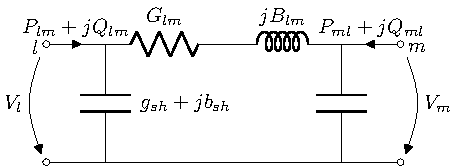
\includegraphics{figures/Line_model.pdf}
            \caption{Two-port $\pi$ model of a branch in distribution grid \cite{gomez2004power}}
        \label{fig:Line_model}
    \end{figure}
\bigskip

\subsection{Measurement Function} \label{subsec:h}

The measurement function $h(x)$ is a function which maps the estimated state of the system to the actual measurements. The most commonly used measurements are the line power flows, bus power injections, and bus voltage magnitudes. With the definition of the state of the system in introduced in Sect.~\ref{subsec:state_estimation}, the measurement function $h(x)$ can be written as follows:
    \begin{align} 
    h(x) &=      
        \begin{bmatrix}
            h^V(x)\\[6pt]
            h^{P_{inj}}(x)\\[6pt]
            h^{Q_{inj}}(x)\\[6pt]
            h^{P_{flow}}(x)\\[6pt]        
            h^{Q_{flow}}(x)         
        \end{bmatrix}
        =
        \begin{bmatrix}
            V_{mag}\\[6pt]
            P_{inj}\\[6pt]
            Q_{inj}\\[6pt]
            P_{flow}\\[6pt]        
            Q_{flow}         
        \end{bmatrix}
	    \label{eq:measurement_function}
    \end{align} 
Given the state of the system $x$, the elements in the measurement function can be formulated as follows:
\begin{itemize}
    \item $h^V(x)$ maps the state of the system to the voltage magnitude:
    \begin{align}
        h^V(x) &= V_{mag}
    \end{align}
    \item $h^{P_{inj}}$ and $h^{Q_{inj}}$ maps the state of the system to the real and reactive power injection ,respectively. For example, the active power injection $P_l$ and the reactive power injection $Q_l$ at bus $l$ can be formulated as:
        \begin{align} 
    	    h^{P_{l}} &= P_{l} 
    	    = V_{l} \sum_{m \in N_l}V_{m} \left(G_{lm}\cos{\theta_{lm}} + B_{lm}\sin{\theta_{lm}} \right)
    	    \label{eq:Pinj} \\[1pt]
    	    h^{Q_{l}} &= Q_{l} = V_{l} \sum_{m \in N_l}V_{m} \left(G_{lm}\sin{\theta_{lm}} - B_{lm}\cos{\theta_{lm}} \right)
    	    \label{eq:Qinj}
        \end{align}
    \item $h^{P_{inj}}$ and $h^{Q_{inj}}$ maps the state of the system to the active power flow and reactive power flow ,respectively. For example, the active power flow $P_{lm}$ and the reactive power flow $Q_{lm}$ from bus $l$ to bus $m$ equals to:
        \begin{align} 
    	    h^{P_{lm}} &= P_{lm} = V_{l}^2 \left(G_{lm}+g_{sh} \right)-V_{l}V_{m}\left(G_{lm}\cos{\theta_{lm}} + B_{lm}\sin{\theta_{lm}} \right)
    	    \label{eq:flow_active} \\[1pt]
    	    h^{Q_{lm}} &= Q_{lm} = -V_{l}^2 \left(B_{lm}+b_{sh} \right)-V_{l}V_{m}\left(G_{lm}\sin{\theta_{lm}} - B_{lm}\cos{\theta_{lm}} \right)
    	    \label{eq:flow_reactive}
        \end{align}    
\end{itemize}
, where
$G_{lm} + jB_{lm}$ is the admittance of the branch connected between bus $l$ and bus $m$ and $g_{sh} + jb_{sh}$ is the shunt admittance of the branch connected at bus $l$ or bus $m$ as shown in Fig.~\ref{fig:Line_model}. $N_{l}$ is the set of buses connected to bus $l$. $V_l$ and $V_m$ are the voltage magnitudes at bus $l$ and bus $m$ respectively, and $\theta_{lm}$ represents the phase difference between bus $l$ and bus $m$ \cite{gomez2004power}. 
\bigskip
\\Equations \ref{eq:Pinj} to \ref{eq:flow_reactive} contain the four following variables: active power $P$, reactive power $Q$, voltage magnitude $V$ and phase $\theta$. The above equations show that, under the assumption that all the parameters of the system, such as the impedance of the branches, tap position of the transformer and state of the breakers, and at least two of the four variables are known, the remaining variables can be calculated. Those equations are utilized for both power flow calculation and measurement function in state estimation, and are physical laws that need to be fulfilled. The most typical method for solving the above equations is the Newton-Raphson method (NR) which is used in this project. As mentioned, the above equations are also part of measurement function $h(x)$, which calculate the branch power flow and bus power injection based on the state $x$. In conclusion, the measurement function $h(x)$ can map the state of the system to its bus voltage magnitudes, bus power injection, and power flow, notably measured by the smart meters, based on Equations \ref{eq:Pinj} to \ref{eq:flow_reactive}.

\subsection{Measurement Jacobian Matrix} \label{jacobian_matrix}
The measurement Jacobian matrix $H$ is defined as the first-order partial derivative of the measurement matrix $h$ with respects to the state of the system: 
\bigskip
\begin{align} 
    H(x) &= \frac{\partial h(x)}{\partial x} 
    =      
    \begin{bmatrix}
                \frac{\partial V_{mag}}{\partial \theta} & \frac{\partial V_{mag}}{\partial V} \\[6pt]
                \frac{\partial P_{inj}}{\partial \theta} & \frac{\partial P_{inj}}{\partial V} \\[6pt]
                \frac{\partial Q_{inj}}{\partial \theta} & \frac{\partial Q_{inj}}{\partial V} \\[6pt]
                \frac{\partial P_{flow}}{\partial \theta} & \frac{\partial P_{flow}}{\partial V} \\[6pt]        \frac{\partial Q_{flow}}{\partial \theta} & \frac{\partial Q_{flow}}{\partial V}             
            \end{bmatrix}
    \label{eq:jacobian_matrix} 
\end{align}
The measurement Jacobian matrix has $m$ rows and $n$ columns, where $m$ equals to the number of measurements and $n$ equals to the number of states. To be more specific, the components in the measurement Jacobian matrix can be written as follows \cite{jaman2017implementation}:
\begin{itemize}
    \item The partial derivative of the voltage magnitude can be formulated as:
        \begin{align} 
    	    \frac{\partial V_{mag}}{\partial \theta} &= 0
    	    \label{eq:V_mag_theta} \\[1pt]
    	    \frac{\partial V_{l}}{\partial V_{l}} &= 1
    	    \label{eq:V_mag_l} \\[1pt]
    	    \frac{\partial V_{l}}{\partial V_{m}} &= 0 
    	    \label{eq:V_mag_m} 
        \end{align}
    \item The components of the measurement Jacobian matrix corresponding to active power injection can be expressed as:
        \begin{align} 
    	    \frac{\partial P_{l}}{\partial \theta_l} &= \sum_{m=1}^{N}V_l V_m \left(-G_{lm}\sin{\theta_{lm}}+B_{lm}\cos{\theta_{lm}}\right)-V_l^2 B_{ll}
    	    \label{eq:P_inj_theta_l} \\[1pt]
    	    \frac{\partial P_{l}}{\partial \theta_m} &= V_l V_m \left(G_{lm}\cos{\theta_{lm}}-B_{lm}\sin{\theta_{lm}}\right)
    	    \label{eq:P_inj_theta_m} \\[1pt]
    	    \frac{\partial P_{l}}{\partial V_l} &= \sum_{m=1}^{N}V_m \left(G_{lm}\cos{\theta_{lm}}+B_{lm}\sin{\theta_{lm}}\right)-V_l^2 G_{ll} \\[1pt]
    	    \label{eq:P_inj_V_l}
            \frac{\partial P_{l}}{\partial V_m} &= V_l \left(G_{lm}\cos\theta_{lm}+B_{lm}\sin\theta_{lm} \right) 
    	    \label{eq:P_inj_theta_m}     	    
        \end{align}    
    \item The components of the measurement Jacobian matrix related to the reactive power injection can be derived as:
        \begin{align} 
    	    \frac{\partial Q_{l}}{\partial \theta_l} &= \sum_{m=1}^{N}V_l V_m \left(G_{lm}\cos{\theta_{lm}}+B_{lm}\sin{\theta_{lm}}\right)-V_l^2 B_{ll}
    	    \label{eq:Q_inj_theta_l} \\[1pt]
    	    \frac{\partial Q_{l}}{\partial \theta_m} &= V_l V_m \left(-G_{lm}\cos{\theta_{lm}}-B_{lm}\sin{\theta_{lm}}\right)
    	    \label{eq:Q_inj_theta_m} \\[1pt]
    	    \frac{\partial Q_{l}}{\partial V_l} &= \sum_{m=1}^{N}V_m \left(G_{lm}\sin{\theta_{lm}}-B_{lm}\cos{\theta_{lm}}\right)-V_l^2 G_{ll} \\[1pt]
    	    \label{eq:Q_inj_V_l}
            \frac{\partial Q_{l}}{\partial V_m} &= V_l \left(G_{lm}\sin\theta_{lm}-B_{lm}\cos\theta_{lm} \right) 
    	    \label{eq:Q_inj_theta_m}     	    
        \end{align}
    \item As for the measurement Jacobian matrix entries related to the active power flow on the branches:
        \begin{align} 
    	    \frac{\partial P_{lm}}{\partial \theta_l} &= V_l V_m \left(g_{lm}\sin{\theta_{lm}}-b_{lm}\cos{\theta_{lm}}\right)
   	        \label{eq:P_lm_theta_l} \\[1pt]
       	    \frac{\partial P_{lm}}{\partial \theta_m} &= -V_l V_m \left(g_{lm}\sin{\theta_{lm}}-b_{lm}\cos{\theta_{lm}}\right)
   	        \label{eq:P_lm_theta_m} \\[1pt]
       	    \frac{\partial P_{lm}}{\partial V_l} &= -V_m \left(g_{lm}\cos{\theta_{lm}}+b_{lm}\sin{\theta_{lm}}\right)+2\left(g_{lm}+jg_{sh} \right)V_l
   	        \label{eq:P_lm_V_l} \\[1pt]
      	    \frac{\partial P_{lm}}{\partial V_m} &= -V_l \left(g_{lm}\cos{\theta_{lm}}+b_{lm}\sin{\theta_{lm}}\right)
   	        \label{eq:P_lm_V_m}
        \end{align}        
    \item Elements representing the partial derivative of the reactive power flow with respective to the states:
        \begin{align} 
    	    \frac{\partial Q_{lm}}{\partial \theta_l} &= V_l V_m \left(g_{lm}\cos{\theta_{lm}}+b_{lm}\sin{\theta_{lm}}\right)
   	        \label{eq:Q_lm_theta_l} \\[1pt]
       	    \frac{\partial Q_{lm}}{\partial \theta_m} &= V_l V_m \left(g_{lm}\cos{\theta_{lm}}+b_{lm}\sin{\theta_{lm}}\right)
   	        \label{eq:Q_lm_theta_m} \\[1pt]
       	    \frac{\partial Q_{lm}}{\partial V_l} &= -V_m \left(g_{lm}\sin{\theta_{lm}}-b_{lm}\cos{\theta_{lm}}\right)-2\left(b_{lm}+jb_{sh} \right)V_l
   	        \label{eq:Q_lm_V_l} \\[1pt]
      	    \frac{\partial Q_{lm}}{\partial V_m} &= -V_l \left(g_{lm}\sin{\theta_{lm}}+b_{lm}\cos{\theta_{lm}}\right)
   	        \label{eq:Q_lm_V_m}
        \end{align}     
    
\end{itemize}
\\With the help of the equations above, the measurement Jacobian matrix can be derived once the topology and the input voltages are determined. Notice that the measurement Jacobian matrix does not change significantly with respect to the input voltage magnitude and phase due to the fact that the p.u. value of the input voltages are close to the flat start. This means that whose voltage magnitudes are close to 1 p.u. and voltage phases are close to zero. By knowing this property of the measurement Jacobian matrix, the computational burden burden can be relaxed by calculating the measurement Jacobian matrix just once at the beginning with a flat start input.

\section{State Estimation Algorithms} \label{subsec:state_estimation}
In this section, the mathematical formulation of four state estimation algorithms, namely WLS, EKF, SHGM, and SVR-EKF will be introduced. All these algorithms except SVR-EKF have already been widely implemented and tested both in simulations and real transmission grid, and the results show that all of them are robust and efficient in the transmission grid. In this thesis they are tested in the low voltage distribution grid and the performance of these algorithms is compared.
\bigskip
\\State estimation is one of the most important functions in EMS. With the help of the great number of measurement devices in transmission grid or pseudo-measurements in the distribution grid, high redundancy can be obtained. This requires state estimation to estimate the most likely state of the system based on noisy, faulty or inaccurate measurements and pseudo-measurements. There are totally three type of measurements in this thesis, including: 
\begin{itemize}
    \item Real measurements from the smart meters which are subject to noise as stated above. The noise of the measurements are determined by the precision of the measurement devices and the surrounding situation. 
    \item Pseudo-measurements are not real measurements but an estimation of the actual value to ensure the observability of the system. Per definition, these are substantially less accurate than real measurements. Details about how to generate pseudo-measurements will be introduced further.
    \item  Virtual measurements are derived from the status of grid components. For example, when there is no load or generator connected to one bus, then the power injection at this bus can be set to zero. If this bus is at the end of one branch, then the power flow across this branch is also zero. To simplify the problem, only the power injection at the buses without load and generator are be treated as virtual buses and the power flow of branches is not considered. This kind of measurements should have higher precision than the real and pseudo-measurements, but for the sake of simplicity, real and virtual measurements are assumed to have the same precision in this thesis.
\end{itemize}
\bigskip
\\With the help of the above measurements, the most likely state of the system is estimated in the DMS. Typically, the state estimator has the following functions
\cite{gomez2004power}: 
\begin{itemize}
    \item Topology processor: Determine the topology of the system and build the single phase or three-phase diagram based on the collected data about the status of circuit breakers and switches.
    \item Observability check: Identify the observability of the system based on the existing measurements. If the system is unobservable, the unobservable lines and observable islands should be identified.
    \item State estimation: Find the optimal state of the system by minimizing the difference between the estimated value and the measurements. The state of the system is defined as the voltage magnitude and phase of each bus. And bus one is defined as the slack bus whose phase is set to zero and assumed to be known in advance. For example, the state $x$ of a system with $N$ number of buses is:
        \begin{align} 
    	    x &=  [\theta_{2} \quad \theta_{3} \quad \cdots \quad \theta_{N} \quad V_{1} \quad V_{2} \quad \cdots \quad V_{N} ]^\intercal
    	    \label{eq:state} 
        \end{align}
   
    \item Bad data processing: Firstly, the bad data detection should be executed among the measurements. Bad data are either eliminated or corrected. However, bad data detection and identification are not investigated in this thesis. The main reason is that there is a great proportion of pseudo-measurements across all measurements to allow the system to be observable. All these pseudo-measurements are very likely to be detected as bad data, and the system is not observable if all these pseudo-measurements are eliminated.
    \item Parameter and structure error processing: Detect the possible parameter and structure errors of the system such as the branches connection error and inaccurate line impedance.
\end{itemize}
\bigskip
\\After estimating the state of the system, the measurements $z$ of the system can be uniquely calculated based on the measurement function $h(x)$ which maps the state x to the measurements z as shown in ~Equation \ref{eq:meas_fun}:
    \begin{align} 
        z &=  \begin{bmatrix}
                    z_{1} \\
                    z_{2} \\
                    \vdots \\
                    z_{m} \\
              \end{bmatrix}
          = \begin{bmatrix}
                    h_1(x) \\
                    h_2(x) \\
                    \vdots \\
                    h_m(x) \\
              \end{bmatrix} +
            \begin{bmatrix}
                    e_1 \\
                    e_2 \\
                    \vdots \\
                    e_m \\
              \end{bmatrix}  
          = h(x)+e
        \label{eq:meas_fun}
    \end{align}
\\, where:    
\begin{itemize}
    \item $z$ is the measurements vector with $m$ number of measurements.
    \item $h_i(x)$ is the non-linear measurement function which maps the state vector $x$ to $i^{th}$ measurement $z_i$. 
    \item $h(x)=\begin{bmatrix}
                    h_{1}(x) &
                    h_{2}(x) &
                    \cdots &
                    h_{m}(x) 
              \end{bmatrix}^\intercal$ 
    \item $e=\begin{bmatrix}
                e_{1} &
                e_{2} &
                \cdots &
                e_{m} 
          \end{bmatrix}^\intercal$.          
    \item $e_{i}$ represents the error between the real value of measurement $h_{1}(x)$ and the measurement from the meter $z_i$ due to the limited accuracy of the meter, a faulty measurement or a pseudo-measurement
    \end{itemize}
    \\The error from meters is assumed to be a white Gaussian noise with zero mean $\mu_{noise}$ and standard deviation $\sigma$. As a result, the error should have the following statistic properties\cite{gomez2004power}:
    \begin{itemize}
        \item Expected value $E(e_i)=\mu_{noise}$ for $i=1,2,...m$.
        \item The errors of each measurement are independent from each other, which means $E(e_i e_j)=0$ for $i=1,2,...m$, $j=1,2,...m$. Thus, the covariance matrix is $R=Cov(e)=E(e\cdot e^\intercal)=diag \big\{ \sigma_{1}^2, \sigma_{1}^2, \cdots, \sigma_{m}^2\big\}$ which reflect the accuracy of measurements.
    \end{itemize}  
\\Based on the assumptions above, the normal probability density function of the measurement vector $z$ can be written as:
\begin{align}
    f\left(z \right) &= \frac{1}{\sqrt{2\pi}\sigma}e^{-\frac{1}{2}\left(\frac{z-\mu}{\sigma}\right)^2}
    \label{eq:pro_den_fun}
\end{align}
, where
\begin{itemize}
    \item $\mu$ is the expected value of the measurement.
    \item $\sigma$ is the standard deviation of the measurement $z$.

\end{itemize}


\subsection{Weigted Least Squares}
\\Weighted Least Squares (WLS) is currently the most widely used state estimation algorithm in the transmission grid due to its high robustness and low computational burden. The object of WLS to obtain the most likely state of the system or to minimize the sum of the weighted squares of the residual $r$, which is defined as the difference between the estimated measurements and the actual measurements from the meters:
\begin{align}
    r &= z-h(x)
    \label{eq:residual}
\end{align}
\subsubsection{Objective Function Formulation}
\\Considering that the normal probability density function of measurements are independent from each other, the joint probability density function of the system with $m$ measurements can be written as:
\begin{align}
    f_m(z) &= f(z_1)f(z_2) \cdots f(z_m)
    \label{eq:likelihood}
\end{align}
,where $f_m(z)$ is the probability density function of the $m$ measurements which shows the probability of the system to be at the state $z$. And the goal is to maximize $f_m(z)$ by tuning the variable $\mu$ and $\sigma$ stated in Equation \ref{eq:pro_den_fun}. Before solving the objective function, a modification is applied to Equation \ref{eq:likelihood} by adding a logarithm ahead of the equation, which is called Log-Likelihood function $\mathcal{L}$:
\begin{align}
    \mathcal{L} &=\log f_m(z) 
    = -\frac{1}{2} \sum_{i=1}^{m} \left(\frac{z_i-\mu_i}{\sigma_i} \right)^2-\frac{m}{2}\log 2\pi- \sum_{i=1}^{m} \log \sigma_i
    \label{eq:log_likelihood}
\end{align}
In Equation \ref{eq:log_likelihood}, the last two elements are constant values which can be neglect, together with the constant factor ahead of the first element, when solving the optimization problem. Hence, the new objective function $J$ can be re-written as:
\begin{equation}
    \begin{aligned}
    & \underset{x}{\text{minimize}}
    & & J(x)=\sum_{i=1}^{m} W_{ii} {r_i} ^2 \\
    & \text{subject to}
    & & r_i = z_i-h_i(x), \; i = 1, \ldots, m.\\
    \label{eq:obj_fun_WLS}
    \end{aligned}
\end{equation}
, where $W_{ii}=\frac{1}{\sigma_{i}^2}$ is $i_{th}$ element of the diagonal weight matrix $W$.   

\subsubsection{Solution of WLS}
\\To find the solution of Equation \ref{eq:obj_fun_WLS}, the first-order optimality condition is sufficient to satisfy the minimization problem \cite{gomez2004power}:
\begin{align}
    g(x) &= \frac{\partial J(x)}{\partial x} 
          = -H^\intercal(x) W (z-h(x))
          =0
    \label{eq:min_der_WLS}      
\end{align}
\\, where $H$ is the measurement Jacobian matrix defined in Equation \ref{eq:jacobian_matrix}. To solve non-linear Equation \ref{eq:min_der_WLS}, Taylor series expansion is applied around the variable $x^k$:
\begin{align}
    g(x) &= g(x^k)+G(x^k)(x-x^k)+\cdots =0
    \label{eq:tyalor_series_g}
\end{align}
, where $G(x^k)$ is called the Gain matrix and formulated as:
\begin{align}
    G(x^k) &= \frac{\partial g(x^k)}{\partial x}
    =H^\intercal(x^k) W H(x^k )
    \label{eq:gain_matrix}
\end{align}
After neglecting the higher order elements in Equation \ref{eq:tyalor_series_g}, the equation goes into a form which can be solved with Gauss-Newton algorithm for minimizing the cost function iteratively:
\begin{align}
     \Delta x^{k+1} &= -[G(x^k)]^{-1} g(x^k)
    \label{eq:WLS_GN}
\end{align}
, where:
\begin{align}
     \Delta x^{k+1} &= x^{k+1}-x^k
    \label{eq:delta_x}
\end{align}
The iteration can be stopped when $\Delta x^{k+1}$ is smaller than a predetermined threshold or the iteration number exceeds a certain number. Because both the measurement Jacobian matrix $H$ and Gain matrix are usually sparse, the Gain matrix $G$ in Equation \ref{eq:WLS_GN} can be ill-conditioned and not invertible. As a result, matrix decomposition skills are utilized to solve Equation \ref{eq:WLS_GN} in a more robust and fast way. Cholesky decomposition is used in this project for solving the equations which contain the inverse of Gain matrix \cite{gomez2004power}. 

\subsection{Extended Kalman Filter}
\label{sect:EKF}
\\In order to make use of the availability of the historical data during state estimation, Dynamic State Estimation (DSE) algorithms are developed for improving the accuracy of the estimator by considering both the real-time data and prediction based on the historical data. Kalman Filter techniques are introduced into state estimation for enhancing the performance of the traditional WLS. There are two typical algorithms proposed with Kalman Filter, Extended Kalman Filter (EKF) \cite{jaman2017implementation} and Unscented Kalman Filter (UKF) \cite{valverde2011unscented}. In this project, EKF is selected as the tested DSE algorithm which includes three main steps of parameter identification, state forecasting, and state correction. EKF is preferred over UKF in this thesis since it has a lower computational burden on Matlab.
\bigskip
\\Assuming the system is operated under quasi steady-state condition, the behavior function of the system can be described as:
\begin{align}
    x_{t+1} &= F_t x_t + g_t +u_t
    \label{eq:quasi_steady_state behaviour function}
\end{align}
, where $t$ is the time sample, $x$ is the state vector, $F_t$ represents the state transition function, vector $g_t$ is associated with the behavior trends of the state trajectory and vector $u_t$ denotes the uncertainty with zero mean and covariance matrix $Q_t$.

\subsubsection{Parameter Identification}
During the first step before forecasting, the values of parameters $F_t$, $g_t$ and $q_t$ should be determined. The white Gaussian noise uncertainty matrix is adjusted by the user, in this project the diagonal elements of the uncertainty matrix are set to 10. In addition, Holt's linear exponential smoothing technique is applied to calculate $F_t$, $g_t$, which is a simple method for short-term time series prediction \cite{da1983state}. The advantage of this forecasting method is that only a small number of historical time step data is used for prediction which reduces the computational burden. To be more specific, these two parameters can be calculated as:
\begin{align}
    F_t &= \alpha_t (1+ \beta_t) I 
    \label{eq:quasi-transition matrix}\\[1pt]
    g_t &= (1+\beta_t)(1-\alpha_t)\widetilde{x}_t-\beta_t a_{t-1} + (1-\beta_t)b_{t-1}
    \label{eq:behaviour_trend matrix}
\end{align}
, where $\alpha_t$ and $\beta_t$ are smoothing parameters at time step $t$ lying between 0 and 1, and they should also satisfy the condition $\alpha_t$ > $\beta_t$. In this project, these two parameters are set to 0.97 and 0.02 for all time steps, respectively. $I$ represents the identity matrix and $\widetilde{x}_t$ means the forecast state at time step $t$. Parameters $a_t$ and $b_t$ are the level and trend at time step $t$, where level index gives an estimate of the local mean and trend represents the change between two successive time steps. They can be obtained by the following equations:
\begin{align}
    a_t &= \alpha_t \hat{x}_t + (1-\alpha_t) \widetilde{x}_t 
    \label{eq:EKF_parameter_a}\\[1pt]
    b_t &= \beta_t (a_t - a_{t-1})+(1-\beta_t)b_{t-1}
    \label{eq:EKF_parameter_b}
\end{align}
, where $\hat{x}_t$ is the estimated state value at time step $t$. With the help of the above equations, the state of the system at the next time step can be predicted.

\subsubsection{State Prediction}
\\After the parameter identification stage, the state of next time step $\widetilde{x}_t$ together with its covariance matrix $P_{\widetilde{x}_t}$ can be predicted:
\begin{align}
    \widetilde{x}_t &= F_t \hat{x}_t +g_t \label{eq:EKF_forecasting_state}
    \\[1pt]
    P_{\widetilde{x}_{t+1}} &= F_t P_{\hat{x}_t} F_t^\intercal +Q_t 
    \label{eq:EKF_forecasting_state_covariance_matrix}
\end{align}
, where $P_{\hat{x}_t}$ is the covariance matrix of predicted state $\hat{x}_t$ at time step $t$. It should be noticed that  $\hat{x}_t$ and $\widetilde{x}_t$ do not include the voltage phase at the feeder bus in Equation \ref{eq:EKF_forecasting_state} and is added after the prediction stage as 0.
\bigskip
 \\In the state estimation, the states which need to be predicted are the voltage phases and voltage magnitude. This forecasting method is more suitable for quasi-steady state. The performance of Holt's linear exponential smoothing technique is not satisfied when the state of the system changes significantly between each time step. In this case, some other forecasting techniques are derived such as Artificial Neural Network (ANN) and Support Vector Regression (SVR).

\subsubsection{State Correction}
In the state correction stage, the state of the system $\hat{x}_{t+1}$ should be estimated based on the measurement $z$ at time step $t+1$ and the forecasted state $\widetilde{x}_{t+1}$. The following objective function can be formulated to calculate the state vector:
\begin{align}
    J(\hat{x}_{t+1})=[z-h(\hat{x}_{t+1})]^\intercal W [z-h(\hat{x}_{t+1})] + (\hat{x}_{t+1}-\widetilde{x}_{t+1})^\intercal P^{-1}_{\widetilde{x}_{t+1}} (\hat{x}_{t+1}-\widetilde{x}_{t+1})
    \label{eq:EKF_objective_function}
\end{align}
Compared with the objective function of WLS in Equation \ref{eq:obj_fun_WLS}, the objective function of EKF considers the influence from both the measurement $z$ collected at time step $t+1$ and the prediction $\widetilde{x}_{t+1}$ made at time step $t$. To solve the minimization problem in Equation \ref{eq:EKF_objective_function}, the Taylor expansion method and first-order optimality condition can be applied similarly to WLS as follows:
\begin{align}
    x^{k+1} &= x^k +K_{t+1} (z-H_{t+1} \widetilde{x}_{t+1})
    \label{eq:EKF_first_order}
\end{align}
, where $K_{t+1}$ is the Kalman gain at time step $t$ defined as:
\begin{align}
    K_{t+1} &= P_t H_{t+1}^{\intercal} R^{-1}
    \label{eq:EKF_kalman_gain}
\end{align}
$k$ is the iteration number. In EKF algorithms, only one iteration is applied as a trade-off between the computational burden and the accuracy of the result. In this project, the weight matrix $W$ in Equation \ref{eq:EKF_kalman_gain} is calculated by Cholesky decomposition. As for the error covariance matrix $P_{\hat{x}_{t+1}}$ of the estimated state, it can be obtained by:
\begin{align}
    P_{\hat{x}_{t+1}} &= \left(H^\intercal R^{-1} H + P_{\widetilde{x}_{t+1}}^{-1} \right)^{-1}
    \label{eq:estimated_state_covraicne_matrix}
\end{align}
Note that EKF needs several time steps to converge if flat start is used as starting point, i.e. initial voltage magnitudes of one and angles of zero. To make EKF comparable with other algorithms by eliminating the influence of the inaccurate results during the converging time steps, the initial estimated voltage magnitude $\hat{V_1}$ and voltage phase $\hat{\theta}_1$ are set to be one and zero, respectively, but the forecasted voltage magnitude $\widetilde{V}_1$ and $\widetilde{\theta}_1$ is assumed to be a perfect value and the phase angle $\widetilde{\theta}_1$ is set to zero at the first time step. The covariance matrix $P_{\widetilde{x}_1}$ is assumed to be zero at the first time step \cite{jaman2017implementation}. 

\subsection{SHGM}
\\Schweppe-type GM-estimator with the Huber psi-function, abbreviated as SHGM, is an algorithm which adapts the weight matrix considering the influence from the leverage points. A leverage point represents a measurement which has a considerably high influence on the resulting estimated state. In the SHGM algorithm, the leverage points are found with the help of the projection statistics method first, and the weight of the bad leverage points in the cost function are reduced.

\subsubsection{Concepts of Leverage Points}
\\Based on the introduction above, leverage points in power system state estimation are measurements which have a stronger influence on the results compared to other measurements. Assuming each row of the measurement Jacobian matrix $H$ represents one point in a $n$ dimension space where $n$ is the number of states and each element in this row is one dimension, some of the rows $H_i$ in the measurement Jacobian matrix $H$ might lies far away from other rows of the measurement Jacobian matrix, and the corresponding measurements of $H_i$ have a stronger influence than other measurements. The influence of each measurement on the estimated result can be expressed as \cite{gomez2004power}:
\begin{align}
    \hat{z} &= \Lambda z
    \label{eq:hat_matrix_equation}
\end{align}
, where $\hat{z}$ and $z$ are estimated and actual measurements, respectively. $\Lambda$ is called the hat matrix and can be calculated as follows:
\begin{align}
    \Lambda &= H G^{-1} H^{\intercal} W 
    \label{eq:hat_matrix_defination}
\end{align}
, where $G$ is the gain matrix introduced in Equation \ref{eq:gain_matrix}. The value of the diagonal elements in the hat matrix goes from zero to one, and represents the distance of the corresponding row $H_i$ with other rows of measurement Jacobian matrix. When $G_{ii}$ close to one, $H_i$ is far from other rows and likely to be a leverage point. The difference between critical measurements and leverage points is that the system can still be observable when the leverage point is eliminated \cite{gomez2004power}. 
\bigskip
\\Typically, the leverage points are more correlated with the topology and parameter of the grid, the measurement is likely to be a leverage point under following conditions \cite{gomez2004power}:
\begin{itemize}
    \item An injection measurement at bus which is connected to a lot of branches.
    \item Power injection measurements at the bus whose connected branches have very different line impedance.
    \item Power flow measurements whose branch impedance significantly differs from other branches of the system.
    \item Power flow measurement on a branch with short and small reactance.
\end{itemize}
\\As stated before, leverage points have a high impact on the accuracy of an estimator. If the measurement associated with a leverage point is good, the accuracy of the estimator is enhanced. However, if the measurement associated with a leverage point is bad, it may wreck the performance of the estimator \cite{rousseeuw1993alternatives}. As a result, the goal of SHGM is to identify the bad leverage points and reduce their influence on the result by giving them a lower weight. 

\subsubsection{Identify Leverage Points}
\\As the leverage points are defined as outliers in the bulk of points cloud, the leverage points identification in state estimation enables to find the rows of the measurement Jacobian matrix which are far away from other rows. To find the outliers in the measurement Jacobian matrix $H$, the Mahalanobis Distance can be used. Having $m$ as the number of rows of measurement Jacobian matrix $H(x)$ and $\{ l_1,l_2,\cdots,l_m \}$ the normalized rows of $H(x)$ which are calculated as:
\begin{align}
    l &= \sqrt{R^{-1}} H(x)
    \label{eq:normalized jacobian matrix l}
\end{align}
The Mahalanobis Distances of $l_i$ with respect to the rest of the rows is definded as:
\begin{align}
    MD_i &= \sqrt{(l_i-\bar{l})C^{-1}(l_i-\bar{l})}
    \label{eq:Mahalanobis distance}
\end{align}
, where $\bar{l}$ is the center of the normalized rows of measurement Jacobian matrix:
\begin{align}
    \bar{l} &= \frac{1}{m} \sum_{i=1}^{m} l_i
    \label{eq:center of l}
\end{align}
And $C$ is the covariance matrix of $l$ and is calculated as follows:
\begin{align}
    C &= \frac{1}{m-1} \sum_{i=1}^{m} (l_i-\bar{l}) (l_i-\bar{l})^\intercal 
    \label{eq:covar of l}
\end{align}
Assuming $l_i$ are Gaussian distributed, then $MD$ in Equation \ref{eq:Mahalanobis distance} follows a chi-square distribution where a threshold can be determined for identifying leverage points in $MD$. Rousseeuw and Croux proposed a new estimator for increasing the robustness and accuracy, which is called projection statistics \cite{rousseeuw1993alternatives}, and Mili applied the projection statistics method to power system state estimation for identifying the leverage points \cite{mili1996robust}. Projection statistics in state estimation is defined as:
\begin{align}
    PS_i &= \max _{v} \frac{|l_i^{\intercal}v|}{S_m}
    \label{eq:projection statistics}
\end{align}
, where $v=l_j, j=1,...,m$. $S_m$ is a scale estimator which represents the sample standard deviation of the projections of data points $l_i$ on the direction of vector $v$ proposed by Rousseeuw and Croux in \cite{croux1992time} and can be written as follows:
\begin{align}
    S_m &= 1.1926\{\underset{i}{lomed} (\underset{j \neq i}{lomed}| l_{i}^{\intercal}v + l_{j}^{\intercal}v|)\}f_m
    \label{eq:SHGM_Sm}
\end{align}
In Equation \ref{eq:SHGM_Sm}, $lomed$ means the low median of a series of elements and $f_m$ is a sample correction factor introduced in \cite{croux1992time}. This factor can make the scale estimator $S_m$ unbiased and its value is related to the number of measurements. When the number of measurements $m$ is smaller than 9 or even, $f_m$ is 1, otherwise when $m$ is larger than 9 and odd \cite{rousseeuw1993alternatives}:
\begin{align}
    f_m &= \frac{m}{m-0.9}
    \label{eq:SHGM fm}
\end{align}
Note that the nominator in Equation \ref{eq:projection statistics} can sometimes be equal to zero due to the sparsity of measurement Jacobian matrix which leads $PS$ to be infinity. To avoid this problem, the zero elements in $| l_{i}^{\intercal}v + l_{j}^{\intercal}v|$ should be eliminated when calculating the low median value in Equation \ref{eq:SHGM_Sm}.

\subsubsection{Algorithm of SHGM}
\\The first step of SHGM algorithm is the leverage points identification. Because leverage points are mainly related to the topology and parameters of the grid, this process can be achieved as an offline algorithm as long as the topology and parameter of the grid are unchanged. So, a flat start is used when calculating $H$ matrix. After that, the projection statistics $PS$ for each measurement is calculated by Equation \ref{eq:SHGM_Sm}, Equation \ref{eq:SHGM fm} and Equation \ref{eq:projection statistics}. Because $PS$ for measurements follow
chi-square distribution, the measurement $i$ is identified as a leverage point if its $PS_i$ is larger than a threshold of 0.975:
\begin{align}
    PS_i &> b_i = \chi_{v,0.975}^{2}
    \label{eq:PS threshold}
\end{align}
, where $v$ is the freedom of chi-square distribution and equals to the number of non-zero entries in the $i^{th}$ row of measurement Jacobian matrix $l_i$. The leverage points are then be down-weighted according to the amount it exceeds the threshold:
\begin{align}
    w_i &= {\min} \{1, (\frac{b_i}{PS_i})^2\}
    \label{eq:weight of SHGM}
\end{align}
From the above equation, it can be seen that the leverage points are given with a small weight if $l_i$ is far away from the ellipsoid center of $H$. In addition, a lower bound of 0.01 is set for w in this project in order to avoid the numerical instabilities in the estimators iterative solution \cite{rousseeuw1993alternatives}. With the help of the weights defined above, the influence of leverage points can be bounded \cite{mili1996robust}. 
\bigskip
\\After adapting the weights, the objective function is defined as \cite{mili1996robust}:
\begin{equation}
    \begin{aligned}
    & \underset{x}{\text{minimize}}
    & & J(x)=\sum _{i=1}^{m} w_i^2 \rho (r_{Si}) \\
    & \text{subject to}
    & & r_{Si} = \frac{r_i}{\sigma_i w_i}, \; i = 1, \ldots, m.\\
    \label{eq:obj_fun_SHGM}
    \end{aligned}
\end{equation}
, where $\rho$ function is chosen to be quadratic up to a certain value:
\begin{align}
    \rho(r_{Si}) &= \begin{cases}
       \frac{1}{2} r_{Si}^{2} & \text{for } |r_{Si}| \leq c  \\
        c|r_{Si}|-\frac{c^2}{2} &  \text{else} 
    \end{cases}
    \label{eq:SHGM p function}
\end{align}
And the solution of Equation \ref{eq:obj_fun_SHGM} is:
\begin{align}
    \sum_{i=1}^{m} w_i l_i \psi(r_{Si}) &= 0
    \label{eq:SHGM solution of ob fun}
\end{align}
, where $\psi$ equals to the derivation of $\rho$ function with respect to the state $x$, which is called Huber $\psi$ function and can be written as:
\begin{align}
    \psi(r_{Si}) &= \begin{cases}
        r_{Si} & \text{for } |r_{Si}| \leq c  \\
        {c \cdot} {\sign}(r_{Si}) &  \text{else} 
    \end{cases}
    \label{eq:SHGM psi function}
\end{align}
, where $c$ is set to be 2.7 in this project according to \cite{rousseeuw1993alternatives}. Parameter $c$ is a threshold for identifying if the measurement is a leverage point with bad measurement. If measurement $i$ is not a leverage point with bad measurement, then $|r_{Si}|$ is smaller than the threshold $c$ and the weight factor $w_i$ in $r_{Si}$ and $w_i$ in Equation 2.62 cancel out \ref{eq:SHGM solution of ob fun}. Note that the objective function is behaved like WLS problem in this case. When $r_{Si}$ is larger than $c$, $|r_{Si}|$ is identified as a leverage point with bad measurement and the weight of the corresponding measurement is reduced. In this case, the objective function behaves like a Weighted Least Absolute Value problem \cite{singh1994weighted}.  
\bigskip
\\After building the objective function of SHGM, the Iteratively Reweighted Least Squaress (IRLS) algorithm is applied to solve the objective function. By dividing and multiplying Equation \ref{eq:SHGM solution of ob fun} by $r_{Si}$, one obtains \cite{mili1996robust}:
\begin{align}
    H^{\intercal}R^{-1}Qr &= 0
    \label{eq:SHGM_IRLS}
\end{align}
, where:
\begin{align}
    Q &= \mathrm{diag}[q(r_{Si})]\\[1pt]
    \label{eq:SHGM Q}
    q(r_{Si}) &= \frac{\psi(r_{Si})}{r_{Si}}
    \label{eq:SHGM q}
\end{align}
By implying first order Taylor expansion on $h(x)$ in $r$ as shown in Equation \ref{eq:residual} and substituting it into Equation \ref{eq:SHGM_IRLS}, the following equation can be obtained:
\begin{align}
    \Delta x^{k+1} &= [(H^k)^{\intercal} R^{-1} Q^k H^k]^{-1} (H^k)^{\intercal} R^{-1} Q^k r^k
    \label{eq:SHGM IRLS}
\end{align}
After getting $\Delta x^{k+1}$ in Equation \ref{eq:SHGM IRLS}, the iteration can start until $\Delta x^{k+1}$ is smaller than the threshold $\epsilon$ or the iteration number $k$ is larger than a threshold of 100 \cite{mili1996robust}. 

\subsection{Support Vector Regression based Extended Kalman Filter}
\\In this section, a newly designed algorithm is introduced here which is a combination between multi-output least squares support vector regression (MLS-SVR) \cite{xu2013multi} and EKF which is abbreviated as SVR-EKF. The multi-output support vector regression machine is utilized to estimate the voltage magnitude and the voltage phase angle is calculated by EKF.

\subsubsection{Support Vector Regression}
\\Support Vector Regression (SVR) is a supervised learning algorithm for regression, which is firstly developed by Vladimir and Alexey in 1963. In 1992, Bernhard, Isabelle, and Vladimir suggested a way to create nonlinear classifiers by applying the kernel trick to maximum-margin hyperplanes \cite{bennett2000support}. Compare to the traditional linear regression method which requires selecting and combining variables or features in advance to transform into a higher dimension, SVR can map the input variables automatically to a higher or even infinite dimension with the help of kernel functions. In the single-output case, traditional SVR does regression with single output separately and independently thus neglecting the relationship between the outputs variables. The advantages of multi-output SVR are thus to consider the cross relationship between outputs by mapping all the inputs to the whole outputs.
\bigskip
\\Assume $\mathbb{R}$ and $\mathbb{R}_+$ represent real numbers and positive real numbers respectively. $\mathbb{N}_n$ means the set of integers from 1 to n. For the single output SVR, the goal is mapping the input variable $x$ to the output $y$. So $x_i$ and $x_i^j$  means the $i^{th}$ vector and $j^{th}$ element in vector $x_i$, respectively. Assuming the size of the training data set is $l$ which means there are $l$ time steps data, the objective function of SVR is \cite{xu2013multi}:
\begin{equation}
    \begin{aligned}
    & \underset{ w,b}{\text{minimize}}
    & & J(w, \xi)= \frac{1}{2} \langle w^{\intercal} \,, w \rangle +\gamma \frac{1}{2} \xi^{\intercal} \xi \\
    & \text{subject to}
    & & y = \langle  Z^{\intercal} \,, w \rangle + b 1_d+\xi\\
    \label{eq:obj_fun_Single_SVM}
    \end{aligned}
\end{equation}
, where $w \in \mathbb{R}^{n_h}$ and $b \in \mathbb{R}$ are variables over which the objective function should be minimized, and $\langle \,, \rangle$ represent the inner product between two vectors or between vector and matrix. $\langle  Z^{\intercal} \,, w \rangle + b 1_d $ in Equation \ref{eq:obj_fun_Single_SVM} is the hyper plane indicting the predicted regression of the data. $\xi$ is the vector form of slack variable with $l$ dimension which represents the orthogonal distance away from the hyper plane and $\gamma$ is a positive real parameter for the penalty between $w$ and $\xi$. If $\gamma$ has a high value, the objective function gives higher weight on $\xi$ and leads to a lower value of $\xi$. However, when $\gamma$ is small, $w$ obtains a higher weight compared to $\xi$ and the hyper plane is more flat in order to avoid the overfitting problem. Figure \ref{fig:single_SVR} shows a schematic diagram of SVR where the bold line in the middle is the hyper plane and $\varepsilon$ is the margin which is set to zero according to \cite{xu2013multi}.
    \begin{figure}[!h]
        \centering
        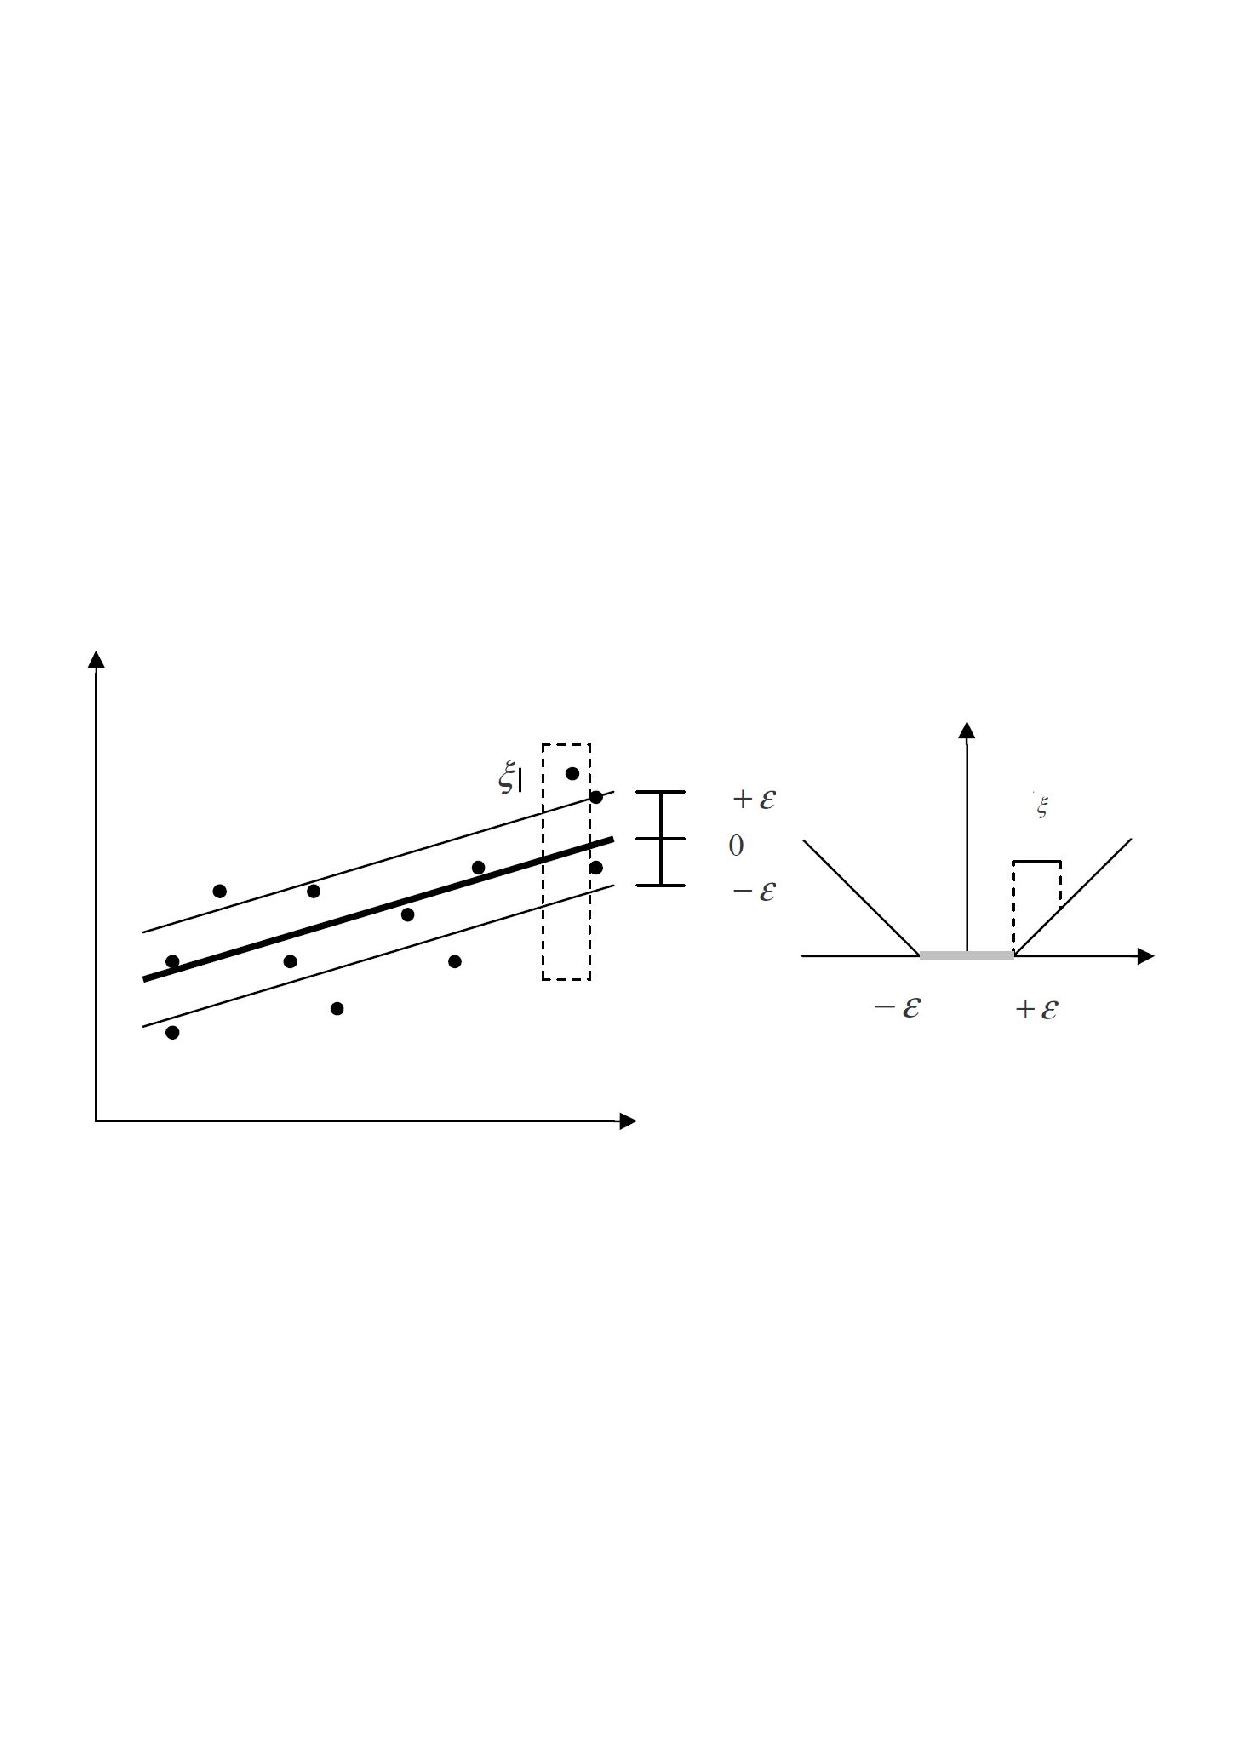
\includegraphics[ height=6.5cm, width=12cm]{figures/SVR.pdf}
        \caption{Support Vector Regression \cite{basak2007support}}
        \label{fig:single_SVR}
    \end{figure}
\bigskip
\\$1_d=[1,1,\cdots,1]^{\intercal} \in \mathbb{R}^d$ and the superscript such as $n_h$ and $d$ represents the dimension of vectors.  And $Z=[\varphi (\textbf{x}_1), \varphi (\textbf{x}_2), \cdots , \varphi (\textbf{x}_l)] \in \mathbb{R}^{n_h \times l}$ who has a inner function $\varphi$ which maps vector $\textbf{x}$ to some high Hilbert space from $d$ dimension to $n_h$ dimension. To solve the above objective function in Equation \ref{eq:obj_fun_Single_SVM}, Karush-Kuhn-Tucker (KKT) condition method is applied by assigning a Lagrange vector $\alpha = (\alpha_1, \alpha_2,\cdots,\alpha_l)^{\intercal}$ to the constraints, which contain one Lagrange multiplier for each constraint. After applying KKT condition method and some further manipulation, the objective function in Equation \ref{eq:obj_fun_Single_SVM} can be transformed into following form \cite{xu2013multi}:
\begin{align}
    \begin{bmatrix} 0 & 1_l^{\intercal} \\ 1_l^{\intercal} & X \end{bmatrix} 
    \begin{bmatrix} b \\ \alpha \end{bmatrix} &=
    \begin{bmatrix} 0  \\ y \end{bmatrix}
    \label{eq:single_SVM_solution}
\end{align}
, where $X = K + \gamma^{-1} I_{-1}$ and $K=Z^{\intercal} Z \in \mathbb{R}^{l \times l} $. The element of the $i^{th}$ row and $j^{th}$ column in matrix $K$ can be written as \cite{suykens2002least}:
\begin{align}
    K_{i,j} &= {\varphi(\mathbf{x}_i)}^{\intercal} {\varphi(\mathbf{x}_j)} 
    = \kappa({\mathbf{x}_i} \,, \mathbf{x}_j)
    \label{eq:SVM kernel func}
\end{align}
, where $\kappa({\mathbf{x}_i} \,, \mathbf{x}_j)$ represents the kernel function which shows the same result with ${\varphi(\mathbf{x}_i)}^{\intercal} {\varphi(\mathbf{x}_j)}$ under Mercer's theorem. There are several kernel functions such as Gaussian kernel, Cosine kernel, and radial basis function kernel(RBF) which is selected in this project. By utilizing the kernel function, new features are generated automatically which transform the linear model into a nonlinear model, and the new dimensions in Hilbert space are dependent on the type of the kernel function. To better solve the Equation \ref{eq:single_SVM_solution}, some reformulation is applied which is introduced in \cite{suykens2002least}:
\begin{align}
    \begin{bmatrix} s & 0_l^{\intercal} \\ 0_l^{\intercal} & X \end{bmatrix} 
    \begin{bmatrix} b \\ \alpha + b X^{-1} 1_l \end{bmatrix} &=
    \begin{bmatrix} 1_l^{\intercal} X^{-1} y   \\ y \end{bmatrix}
    \label{eq:single_SVM_solution_revised}
\end{align}
, where $s=1_l^{\intercal} X^{-1} 1_l \in \mathbb{R}_+ $ and the optimal result can be obtained for the objective function in Equation \ref{eq:obj_fun_Single_SVM} which are $\alpha^{*}$, $w^{*}$,  and $b^{*}$. By using the optimal parameters calculated above, the optimal hyper plane can be obtained and the corresponding decision function for making predictions can be built as \cite{xu2013multi}:
\begin{align}
    f_{SVR}(x) &=\langle \varphi (x) ^{\intercal}  \,,  w^{*} \rangle  + b^{*} = \sum_{i=1}^{l} \alpha_i^{*} 
                    \kappa({x_i} \,, x)+b^{*}
    \label{eq:single_SVM_pred}
\end{align}
From the above equation, it can be found that kernel function replace the inner product between the non-linear mapping variable and weight vector which allow the burden from creating non-linear mapping functions \cite{xu2013multi}.

\subsubsection{Multi-output LS-SVR}
\\To consider the correlations between outputs, Multi-output Least-square Support Vector Regression (MLS-SVR) has been developed by Xu \cite{xu2013multi}. When there are totally $m$ outputs,
to transform single-output SVR to MLS-SVR, the elements in the weight vector $w_i$ can be expressed by the sum of two vectors as follows:
\begin{align}
    w_i=w_0+v_i
\end{align}
, where $w_i \in \textbb{R}^{n_h}$ for $i \in \textbb{N_m}$ is the weight vector of the $i^{th}$ output. $w_0$ is called the mean vector which stands for the common part between each $w_i$ for $i \in \textbb{N_m}$ and $v_i$ represents the differences between each $w_i$ for $i \in \textbb{N_m}$. The mean vector $w_0$ is big when the output are similar to each other, otherwise $w_0$ is small. This way, the aim of the optimization problem is finding the optimal value of $w_0 \in \mathbb{R}^{n_h}$, $V = ( v_1, v_2, \cdots, v_m ) \in \mathbb{R}^{n_h \times m} $, and $b = (b_1, b_2, \cdots, b_m) \in \mathbb{R}^{m}$. Based on the assumptions above, the objective function of MLS-SVR can be formulated as follows \cite{xu2013multi}:
\begin{equation}
    \begin{aligned}
    & \underset{ w_0, b, V}{\text{minimize}}
    & & J( w_0, V, \Xi)= \frac{1}{2} \langle w_0^{\intercal} \,, w_0 \rangle +\frac{1}{2} \frac{\lambda}{m} \mathrm{trace} (\langle \Xi^{\intercal} \,, \Xi \rangle) \\ 
    & \text{subject to}
    & & y = \langle  Z^{\intercal} \,, W \rangle + \mathrm{repmat}(b, l, 1 )+\Xi\\
    \label{eq:obj_fun_MLS_SVM}
    \end{aligned}
\end{equation}
, where $ \Xi = ( \xi_1, \xi_2, \cdots, \xi_m ) \in \mathbb{R}^{l \times m}$ are the penalty vector for $m$ outputs, $ W = ( w_1, w_2, \cdots, w_m ) \in \mathbb{R}^{n_h \times m}$, and $\lambda, \gamma \in \mathbb{R}_{n_h}$ are two positive real regularized parameters \cite{xu2013multi}. The function $\mathrm{trace}(A)$ represents the sum of the diagonal elements in square matrix $A$ and the function $\mathrm{repmat}(A, m, n)$ create a new matrix of $m$ rows and $n$ columns whose element is $A$.
\bigskip
\\Similar with LS-SVR, the objective function above can be solved by transforming it into linear equations with the help of KKT condition method. Assuming $\alpha = ( \alpha_{1}^{\intercal}, \alpha_{2}^{\intercal},\cdots,\alpha_{m}^{\intercal} ) \in \mathbb{R}^{ml}$, where $ml = m \times l$, is the vector form of the langrange multiplier for $m$ number of constraints. The function $\mathrm{blockdiag(A_1, A_2,\cdots, A_n)}$ creates a diagonal matrix whose diagonal elements are $(A_1, A_2,\cdots, A_n)$ and the rest elements are zero. After some manipulations, the following equations can be obtained \cite{xu2013multi}:
\begin{align}
    \begin{bmatrix} 0_{ml \times m} & P^{\intercal} \\ P^{\intercal} & X \end{bmatrix} 
    \begin{bmatrix} b \\ \alpha \end{bmatrix} &=
    \begin{bmatrix} 0_m  \\ y \end{bmatrix}
    \label{eq:MLS_SVM_solution}
\end{align}
, where $P=\mathrm{blockdiag} (1_l, 1_l,\cdots, 1_l ) \in \mathbb{R} ^{ml \times m}$, $X=\Omega+ \gamma^{-1} I_{ml}+\frac{m}{\lambda} Q \in \mathbb{R} ^{ml \times ml}$, $\Omega=\mathrm{repmat}( K,m,m) \in \mathbb{R}^{m \times m}$, $K= Z^{\intercal} Z \in \mathbb{R}^{l \times l}$ and $y=(y_1^{\intercal}, y_2^{\intercal},\cdots, y_3^{\intercal}) \in \mathbb{R}^{ml}$. After solving Equation \ref{eq:MLS_SVM_solution}, the optimal value $\alpha^*$ and $b^*$ can be obtained thus the corresponding decision function is shown as follows \cite{xu2013multi}:
\begin{align}
    f_{MLS-SVR}(\mathbf{x}) &= 
     \mathrm{repmat}( \sum_{i=1}^{m} \sum_{j=1}^{l} \alpha_{i,j}^{*} 
                    \kappa({x_i} \,, x_j),1,m)+\frac{m}{\lambda} \sum_{j=1}^{l} \alpha_j^*\kappa({x_i} \,, x_j) +{b^{*}}^{\intercal}
    \label{eq:MLS_SVM_regression}
\end{align}
By utilizing the above equations, prediction can be made based on the historical data and parameter $\alpha^*, b^*$. Finally, the MLS-SVR function for prediction can be written as:
\begin{align}
    x_p &= f_{predict} (x_{train},x_{test},\alpha^*, b^*,\lambda,p)
    \label{eq:MLS_SVM_prediction}
\end{align}
, where $x_p$ is the predicted value, $x_{train}$ is the training set and $x_{test}$ is the test set. $p$ is the hyperparameter for the kernel function. $\lambda$ and $p$ can be determined by grid search method with the data in the training set \cite{xu2013multi}.
\subsubsection{SVR-EKF Algorithm}
SVR-EKF is a combined algorithm between SVR and EKF. The basic idea is to estimate the voltage magnitude of the buses based on SVR and estimate the voltage phase angle by EKF. Before estimating the state of the system based on the measurements from the smart meters, it is necessary to generate the training set for the estimation process in SVR. By setting the feeder bus to the slack bus, the voltage magnitude is $1$ $p.u$ and the voltage phase angle is $0$ $rad$ at the feeder bus. In addition, assigning active power injection and reactive power injection at each bus except the slack bus, these buses are treated as PQ buses in the power flow calculation. Assuming there are totally $n$ buses in the system, there is one slack bus and $n-1$ PQ buses, and the power flow calculation can be simulated based on the above information. After the power flow calculation, a situation where all types of measurements, including voltage magnitude, voltage phase angle, power injection at each bus, and power flow at each branch, are known and without error can be obtained.
\bigskip
\\After obtaining the full-knowledge of the system with power flow calculation, the input and output of the training set for SVR should be determined. The input for training SVR are the measurements from the training set in the full-knowledge situation, whose corresponding information in the test set are known in the real system including real meter measurements, pseudo-measurements, and virtual measurements. And the outputs of SVR are voltage magnitudes and voltage phase angle at each bus. Because the performance of SVR is heavily dependant on the training set, the training set should be updated regularly when the difference between the value of the power injections in the training set and the test set increases, such as when more households are equipped with a PV panel and the power injection at the corresponding buses increases. 
\bigskip
\\After obtaining the training set, SVR can be trained and the optimal $\alpha^*$ and $b^*$ can be obtained for predicting the voltage magnitude and phase angle at each bus by Equation \ref{eq:MLS_SVM_prediction}. In the test stage, the input data of the test set are all types of measurements collected from the distribution grid and the prediction can be made based on Equation \ref{eq:MLS_SVM_prediction} whose output are voltage magnitudes and phase angle at each bus. These predicted voltage magnitudes and phase angle by SVR are then sent to EKF firstly as the predicted state $\widetilde{x}$, which replaces the Holt's linear exponential smoothing technique in Equation \ref{eq:quasi_steady_state behaviour function}, to estimated the state of the distribution grid at time step $k+1$. After getting the predicted state $\widetilde{x}_{k+1}$ by SVR, EKF is run based on the equations introduced in Sect.~\ref{sect:EKF} except the step for calculating the state transition function $F_k$ at time step $k$ in Equation \ref{eq:quasi-transition matrix}, which is instead calculated as follows:
\begin{align}
    F_k &= \widetilde{x}_{k+1} \hat{x}_k^{-1}
    \label{eq:SVM transtion function}
\end{align}
, where $\widetilde{x}_{k+1}$ is the predicted state by SVR at time step $k+1$ and $\hat{x}_k$ is the estimated state by SVR-EKF at the $k^{th}$ time step. After the simulation of EKF, the estimated voltage phase angle $\hat{\theta}_{k+1}$ is selected as the final estimated voltage phase angle for time step $k+1$, but the estimated voltage magnitude $\hat{V}_{k+1}$ by EKF is neglected and replaced by the predicted voltage magnitude $\widetilde{V}_{k+1}$ from SVR which is the final estimated voltage magnitude due to its higher accuracy. Figure \ref{fig:flow_chart_SVR} shows the flowchart of the whole procedure of MLS-SVR voltage magnitude prediction process from training to forecasting.
    \begin{figure}[!h]
        \centering
        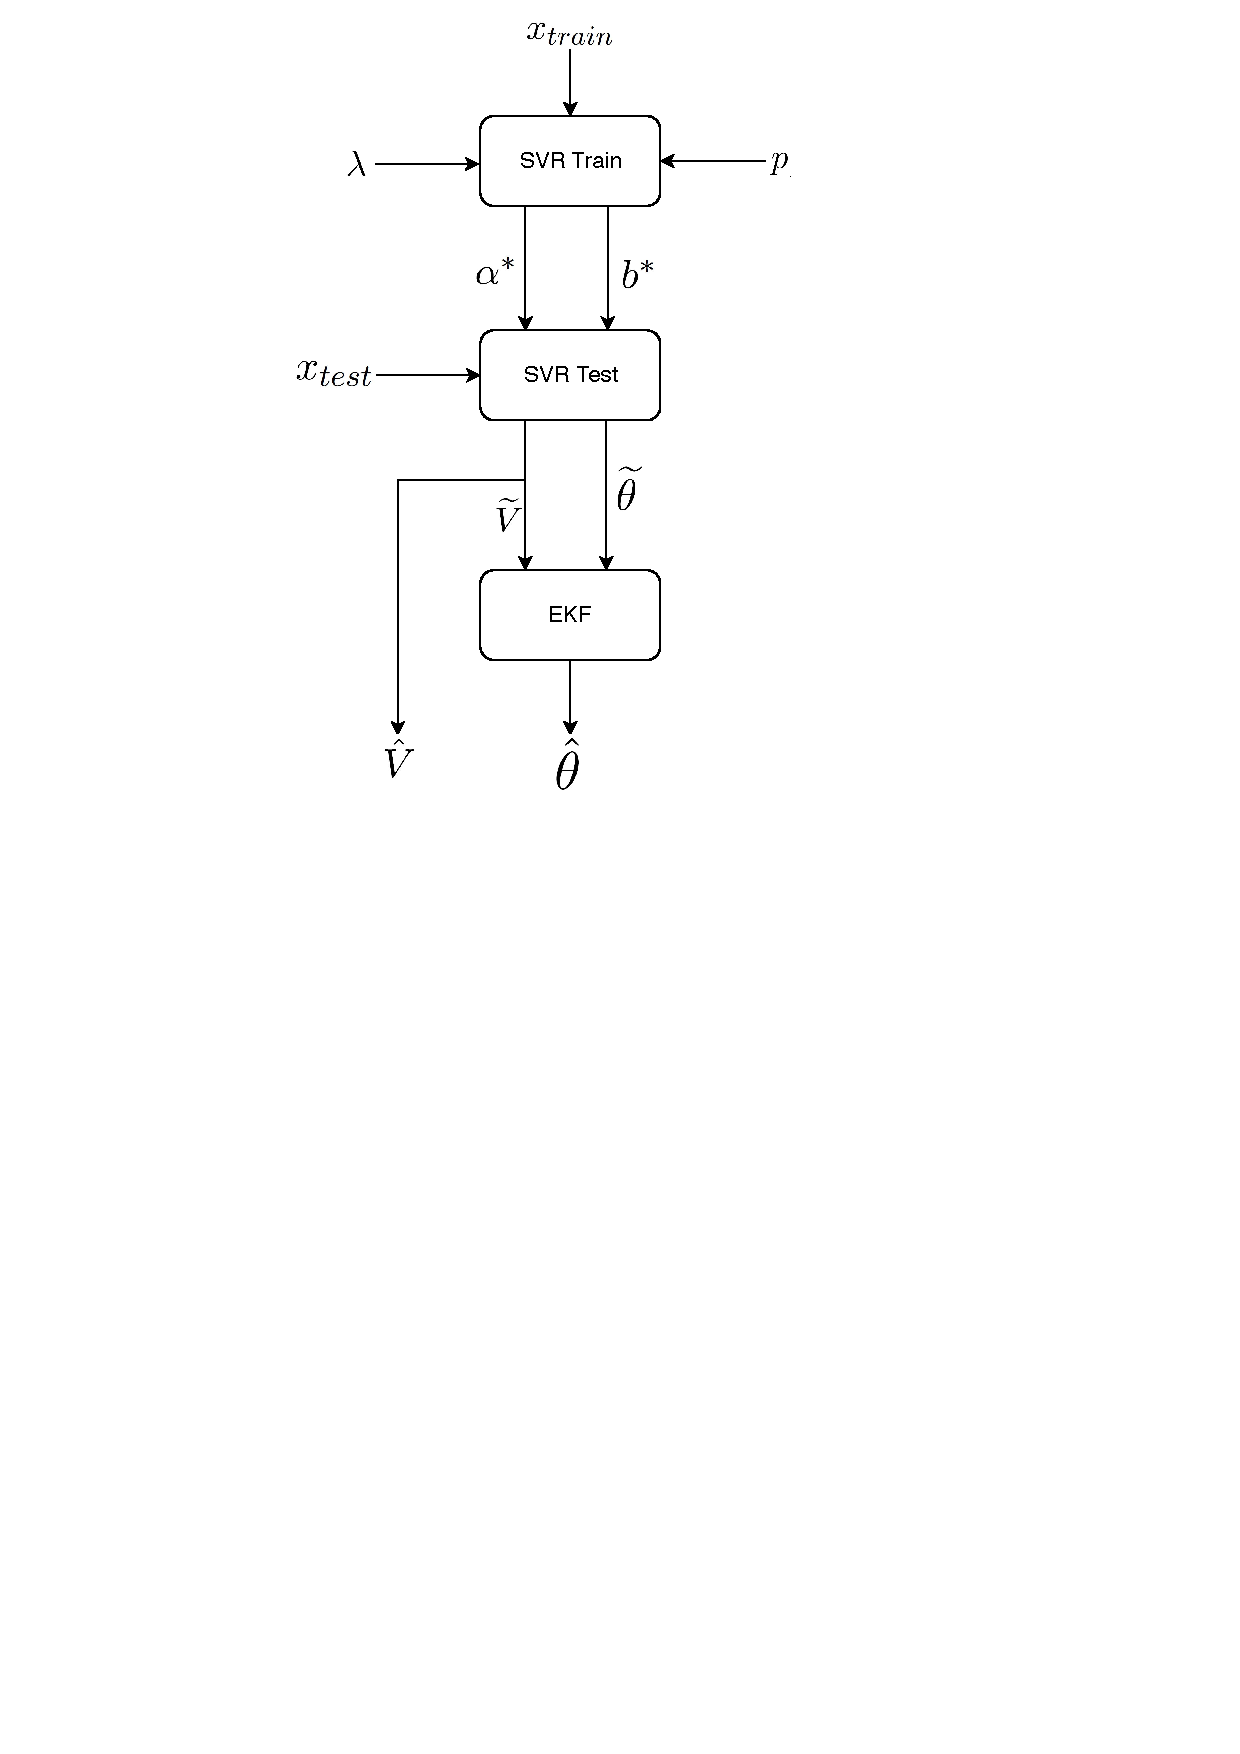
\includegraphics[ height=15cm, width=11cm]{figures/SVR_flow.pdf}
        \caption{Flowchart of SVR-EKF}
        \label{fig:flow_chart_SVR}
    \end{figure}
\bigskip
\\In conclusion, the output voltage magnitudes of SVR are used for both the prediction $\widetilde{V}$ for EKF and the final estimated voltage magnitude $\hat{V}$, whereas the output voltage phase angle of SVR are only used for the prediction stage $\widetilde{\theta}$ for EKF. The estimated voltage phases angle $\hat{\theta}$ is obtained through EKF. The reason why the predicted voltage phase angle from SVR cannot be the estimated value is because the reactive power injection in this thesis is much smaller than the active power injection, which means the voltage phase angles are close to zero and even a small estimated voltage phase error leads to a high estimated power flow error. So, the estimated voltage phase angle from EKF has a higher accuracy compared to the predicted voltage phase angle from SVR in this case.


\newpage
%3
\chapter{Simulation Preparation} \label{chap:Simulation Preparation}
This chapter introduces the system modeling process for preparing the state estimation simulation. During the system modeling section, the topology of the system is built based on a 400V IEEE European test system with 206 buses and 205 branches, and pseudo-measurements are generated to ensure the observability of the system. There are totally 30 scenarios generated for different levels of measurements, where each scenario contains 100 cases with different locations of installed smart meters, distributed by Monta-Carlo simulation. After the modeling of the system, the four state estimation algorithms introduced in Chapter \ref{chap:Math_for} are implemented and tested on this system.

\section{Introduction of Test System}
The test system is a distribution grid with a radial topology. In this project, this system is assumed to be balanced, and the single phase model is used during the simulation. The feeder bus is defined as the slack bus and the base power is set to 1000 VA. Because the distribution grid branches have shorter distance and smaller diameter than the transmission grid, the distribution grid has a high $R/X$ ratio and small line-to-ground capacitance. Thus, the line-to-ground capacitance of the tested distribution grid is assumed to be zero for simplification.
\bigskip
\\There are totally 30 tested scenarios, which can be found in Table \ref{tab:30_scenarios}, with different levels and types of measurements including bus voltage magnitude, bus injection power, and branch power flow. Smart meter measurements are available according to the following rules:
    \begin{table}[!h]
        \centering
        \begin{tabular}{c|c|c|c|c}
            Scenario Index & P Injection & Q Injection & V & Branch Power Flow \\ \hline
            $1$ & $0{\%} $ & 0{\%} & 0{\%} & 0{\%} \\
            $2$ & $0{\%} $ & 0{\%} & 0{\%} & 10{\%} \\ 
            $3$ & $0{\%} $ & 0{\%} & 0{\%} & 20{\%} \\
            $4$ & $33.3{\%} $ & 0{\%} & 0{\%} & 0{\%} \\
            $5$ & $33.3{\%} $ & 0{\%} & 0{\%} & 10{\%} \\ 
            $6$ & $33.3{\%} $ & 0{\%} & 0{\%} & 20{\%} \\
            $7$ & $33.3{\%} $ & 33.3{\%} & 0{\%} & 0{\%} \\
            $8$ & $33.3{\%} $ & 33.3{\%} & 0{\%} & 10{\%} \\ 
            $9$ & $33.3{\%} $ & 33.3{\%} & 0{\%} & 20{\%} \\
            $10$ & $33.3{\%} $ & 33.3{\%} & 33.3{\%} & 0{\%} \\
            $11$ & $33.3{\%} $ & 33.3{\%} & 33.3{\%} & 10{\%} \\ 
            $12$ & $33.3{\%} $ & 33.3{\%} & 33.3{\%} & 20{\%} \\        
            $13$ & $66.6{\%} $ & 0{\%} & 0{\%} & 0{\%} \\
            $14$ & $66.6{\%} $ & 0{\%} & 0{\%} & 10{\%} \\ 
            $15$ & $66.6{\%} $ & 0{\%} & 0{\%} & 20{\%} \\
            $16$ & $66.6{\%} $ & 66.6{\%} & 0{\%} & 0{\%} \\
            $17$ & $66.6{\%} $ & 66.6{\%} & 0{\%} & 10{\%} \\ 
            $18$ & $66.6{\%} $ & 66.6{\%} & 0{\%} & 20{\%} \\
            $19$ & $66.6{\%} $ & 66.6{\%} & 66.6{\%} & 0{\%} \\
            $20$ & $66.6{\%} $ & 66.6{\%} & 66.6{\%} & 10{\%} \\ 
            $21$ & $66.6{\%} $ & 66.6{\%} & 66.6{\%} & 20{\%} \\
            $22$ & $100{\%} $ & 0{\%} & 0{\%} & 0{\%} \\
            $23$ & $100{\%} $ & 0{\%} & 0{\%} & 10{\%} \\ 
            $24$ & $100{\%} $ & 0{\%} & 0{\%} & 20{\%} \\ 
            $25$ & $100{\%} $ & 100{\%} & 0{\%} & 0{\%} \\
            $26$ & $100{\%} $ & 100{\%} & 0{\%} & 10{\%} \\ 
            $27$ & $100{\%} $ & 100{\%} & 0{\%} & 20{\%} \\
            $28$ & $100{\%} $ & 100{\%} & 100{\%} & 0{\%} \\
            $29$ & $100{\%} $ & 100{\%} & 100{\%} & 10{\%} \\ 
            $30$ & $100{\%} $ & 100{\%} & 100{\%} & 20{\%}             
        \end{tabular}
        \caption{30 Scenarios of Measurements}
        \label{tab:30_scenarios}
    \end{table}

\begin{itemize}
    \item The voltage magnitude, voltage phase angle, active and reactive power injection at feeder bus are always known. The voltage magnitude is 1 p.u. and the voltage phase is 0 $rad$.
    \item The reactive power injection at a certain bus is only known if, and only if, the active power injection is also known. Otherwise, only the feeder bus has the information of the reactive power injection.
    \item The voltage magnitude value at a certain bus is only known if, and only if, the active and reactive power injection is also known.  Otherwise, only the information of the voltage magnitude at the feeder bus is known. 
    \item To ensure the observability of the system, pseudo-measurements must be generated when the active or reactive power injection at any bus is unknown. The details about pseudo-measurements generation are introduced in Sect.\ref{sect:pseudo-measurements}
    \item Active and reactive branch power flows are measured together. This means that if the active power flow at a certain branch is known, the information of the reactive power flow on the same branch must also be known.
    \item when determining how much percentage information of the active or reactive power injection is known, the virtual active or reactive power injection are not considered. For example, under the scenario 4 where $33 \%$ of the active power injection information is known, if there are 206 buses in the system and the active power injection of 30 buses have virtual measurements, then the information of $(206-30)\times \frac{33.3}{100} \approx 59$ active power injections are known through the real measurements by smart meters. 
    \item Due to the fact the branch power flow has two directions, there are two possible locations to measure the branch power flow for two power flow directions, from one bus to another and vice versa. Assuming there are 205 branches, $205 \times 2 \times \frac{10}{100} = 41 $ branch power flows are known under $10 {\%}$ power flow scenarios.
\end{itemize}

\section{Measurement Generation}
\subsection{Load Generation}
The original load data are collected from two sources by smart meters. One source is 1000 active power load for small household consumers and another source is 1000 active power injection from PV systems in the City of Basel. Both of them are recorded from April $1^{st}$ 2014 to July $1^{st}$ 2017 with a time interval of 15 minutes between each time step. So, there are totally 96 recorded time steps per day.
\bigskip
\\In order to populate the grid with loads in a realistic way, the following approach has been considered:
\begin{itemize}
    \item For each of the 206 buses in the LV distribution grid, 0 to 5 consumer loads are selected randomly from those 1000 consumers and aggregated together as a new load. This is motivated by the fact that there might be no consumers, a single family house or multiple flats (e.g., multi-family house) connected to a single node
    \item Because of the lack of reactive power consumption data, a constant power factor of 0.98 inductive is used.
    \item Concerning PV generation, 20 of them are selected from the 1000 PV generation profiles and distributed randomly to 20 buses in the distribution system.
\end{itemize}
In this way, the active and reactive power injection at each bus is obtained. Therefore, there are two types of buses in this case: slack bus for the feeder and PQ buses for other buses. Subsequently, a power flow calculation can be run for generating the full-knowledge situation, namely all voltage magnitudes and phase angles, active and reactive power injections, and active and reactive power flows. 
\bigskip
\\Because SVR-EKF needs an extra training set, the power flow calculation introduced above is run twice for generating the training set and the test set separately. The original data ranges from April 2014 to April 2017. The load and PV generation on the first day, which contains 96 time steps with 15 minutes time interval, is selected as the test group for all those four algorithms and noise is added to the measurements as introduced in Sect.\ref{sect:add noise}. The power injection of the training set is selected from the second to fourth day for both loads and PV generation. There is no noise added to the training group for both input and output data, which ensure the accuracy of the SVR in SVR-EKF. 
\subsection{Adding Noise to Measurements}
\label{sect:add noise}
As it is introduced in Chapter \ref{chap:Math_for}, the measurement from the smart meter is not perfect and white Gaussian noise is assumed in each measurement. In this project, a uniform noise is added on the measurements for imitate the white Gaussian noise with a zero mean and 0.01 standard deviation, assuming that inaccuracies are due to the externals environments of the smart meters and have no relationship with the type or value of the measurements. Thus, noise is generated randomly within $[-0.01,0.01]$ for each measurement at each time step which is shown in Equation \ref{eq:measurements with noise}:
\begin{align}
    meas_{noise} &= \epsilon + meas_{ideal}
    \label{eq:measurements with noise}
\end{align}
, where $meas_{noise}$ and $meas_{ideal}$ are measurements with and without noise, respectively. $\epsilon$ is the random number ranging between $-0.01$ and $0.01$ for measurement $meas_{ideal}$. Figure \ref{fig:meas_with_without_noise} gives an intuition of the bus voltage magnitude with and without noise over 96 time steps.
    \begin{figure}[!h]
        \centering
        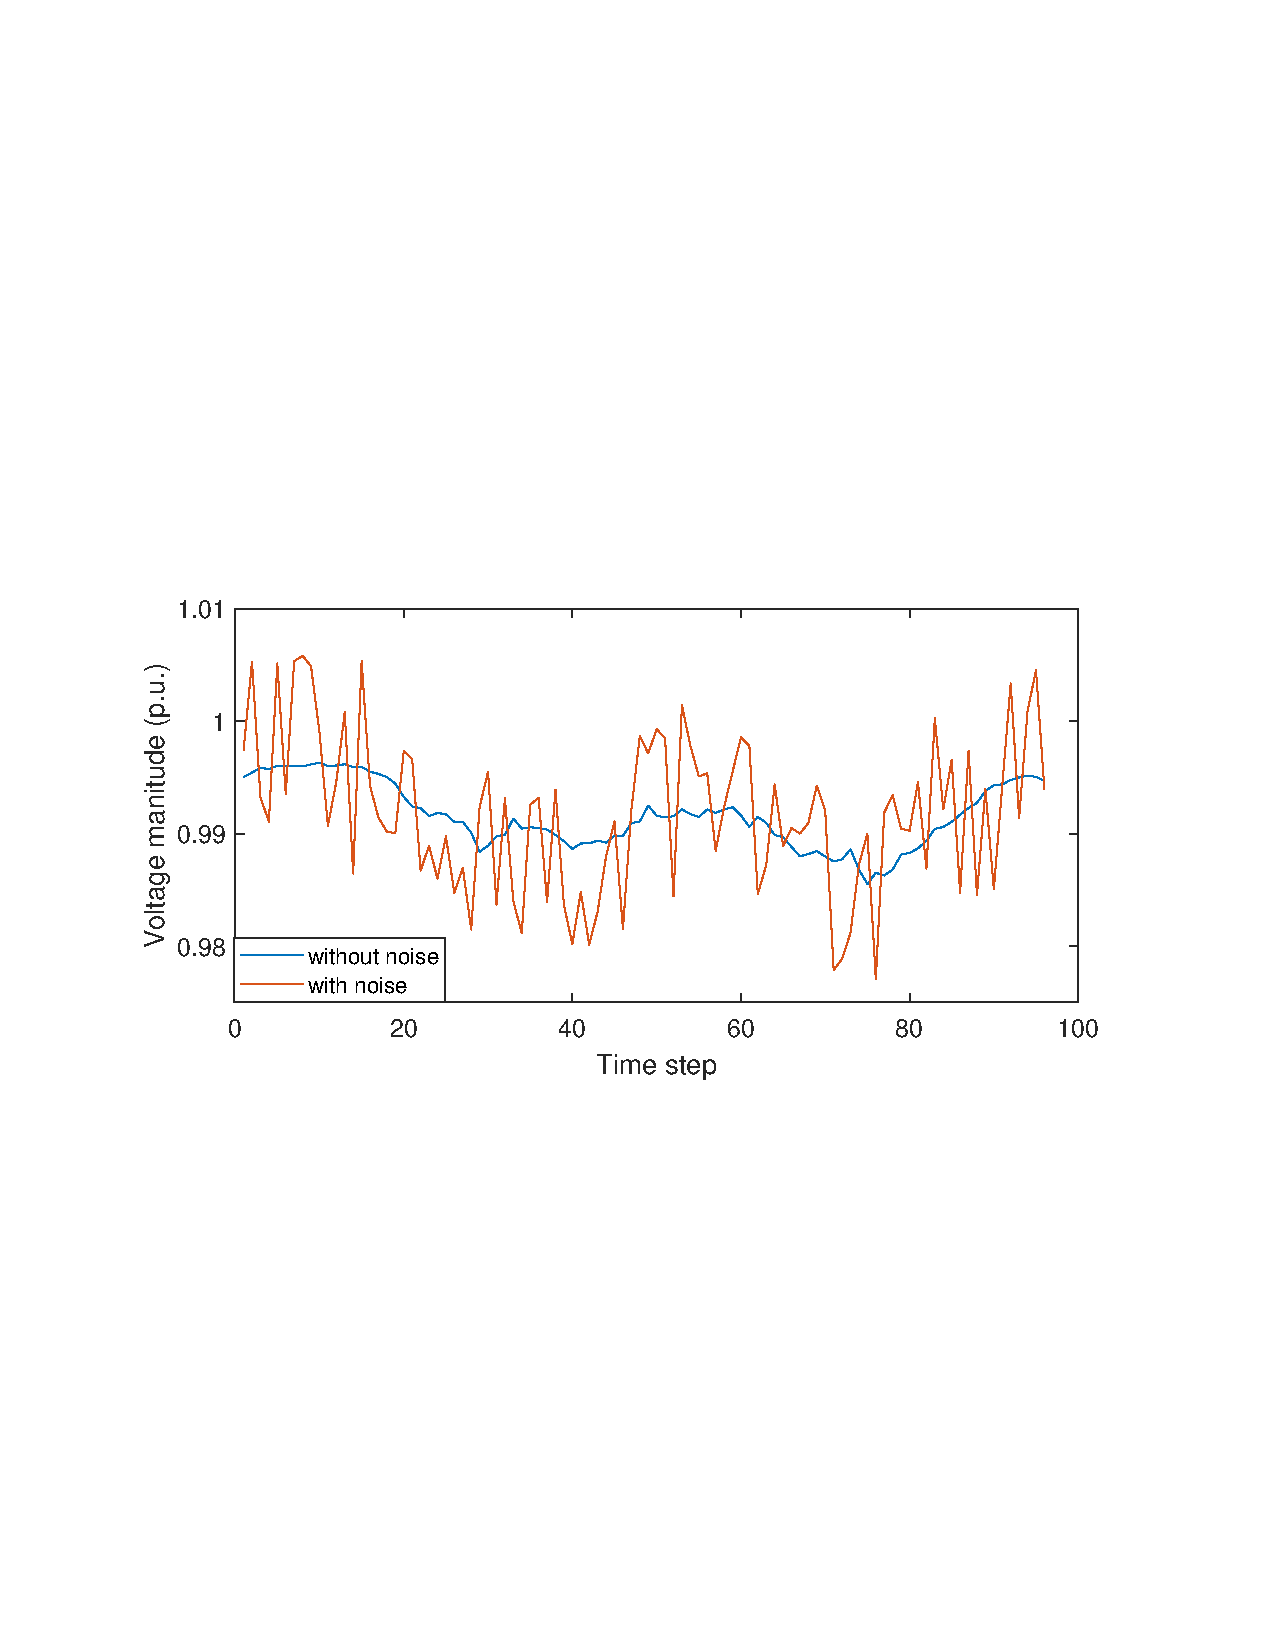
\includegraphics[ height=8cm, width=13cm]{figures/meas_with_without_noise.pdf}
        \caption{Voltage magnitude of bus 2} 
        \label{fig:meas_with_without_noise}
    \end{figure}
    
\subsection{Generation of Pseudo-Measurements}
\label{sect:pseudo-measurements}
To ensure the observability of the system, pseudo-measurements should be generated. To determine if a system is observable or not, one can easily check the rank of the measurement Jacobian matrix $H$ introduced in Equation \ref{eq:jacobian_matrix}. If the rank of the measurement Jacobian matrix is smaller than twice the number of buses, the system is unobservable. Otherwise, the system is observable. There are several existing pseudo-measurements generation methods based on machine learning skills such as SVR and ANN. This thesis generates pseudo-measurements simply based on the proportion of the total energy consumption at each bus. 
\bigskip
\\It is assumed that active and reactive power injection, and voltage magnitude and angle are known at the slack bus in all 30 scenarios.Measurements at buses without load or PV generation are defined as virtual measurements. 
\bigskip
\\The system is observable when the power injection at all buses are known in addition to the voltage magnitude and phase angle at the slack bus. Therefore, to ensure that the system is observable, all buses whose power injection is unknown, are assigned with a pseudo power injection.
\bigskip
\\Nevertheless, the total energy consumption E over the simulation period at each bus is assumed to be known, which is used to generate the pseudo power injection at buses without smart meter. In addition, knowing the active power flow at the slack bus, a measurement gap, which is called active power residual vector $p_r=[p_r^1, p_r^2,\cdots,p_r^{96}]$ for 96 time steps, is observed between this active power profile and the spatial aggregation of all active power profiles measured by smart meters, considering also PV systems as shown by Figure \ref{fig:meas_gap}.
    \begin{figure}[!h]
        \centering
        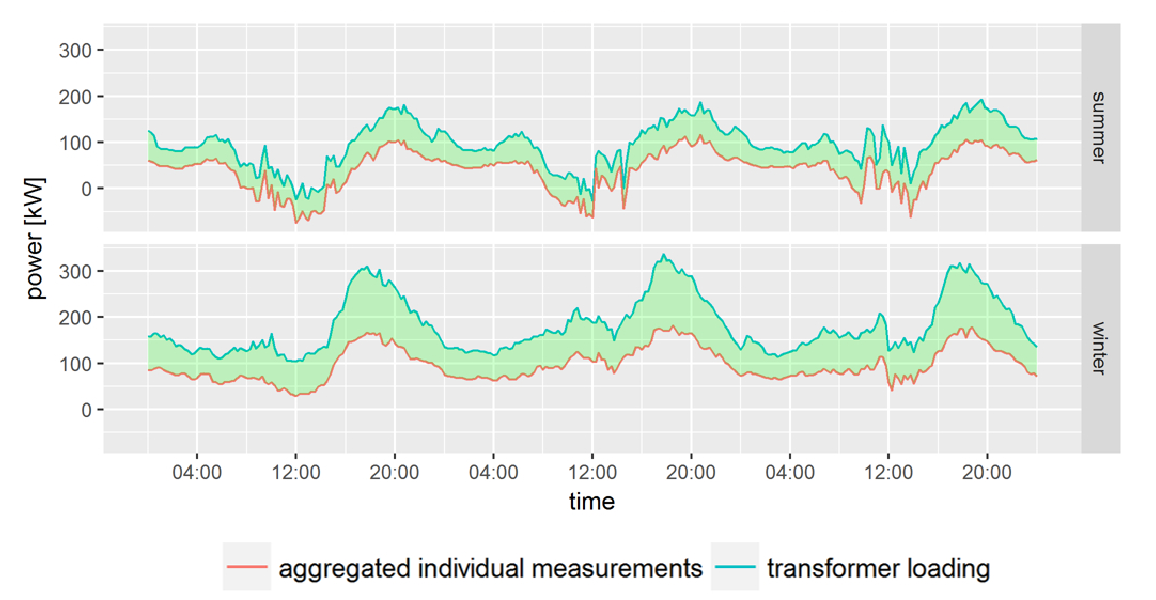
\includegraphics[ height=8.5cm, width=13cm]{figures/measurement_gap.pdf}
        \caption{Power gap between transformer loading and aggregated individual measurements} 
        \label{fig:meas_gap}
    \end{figure}
The green region is the gap corresponds to the aggregated power consumed by loads without smart meter. Pseudo-measurements of reactive power are synthesized similarly. Assuming $p_{inj}=[p_{inj}^1,p_{inj}^2,\cdots,p_{inj}^l]$ is the active power injection for $l$ buses whose active power injection is measured, and $p_{inj}^i=[p_{inj}^{i,1}, p_{inj}^{i,2},\cdots,p_{inj}^{i,96}]$ is the $i^{th}$ measured active power injection for 96 time steps. The active power gap $p_{c}$ in Figure \ref{fig:meas_gap} can be obtained as follows:
\begin{align}
    p_c &= \sum_{i=1}^{l} p_{inj}^i+\sum_{i=1}^{g} p_{gen}^i
    \label{eq:pseudo_power_injection_curve}
\end{align}
, where $p_{gen}=[p_{gen}^1,p_{gen}^2,\cdots,p_{gen}^g]$ is the active power generation from the PV generators, and $g$ is the number of PV generators which equals to 20 in this thesis. Hence, pseudo-measurements are created for each non-measured load by splitting the measurement gap profile into multiple active power profiles (i.e. one profile per non-measured load) according to their total energy consumption $E_c=[E_c^1,E_c^2,\cdots,E_c^p]$, where $p$ is the total number of buses whose active power injection is not measured \cite{ghosh1997load}. Assuming $E_c=[E_c^1,E_c^2,\cdots,E_c^p]$ is the total active energy consumption for the buses without active power measurements, and $p$ is the total number of buses who do not have active power injection information. Then, the pseudo active power consumption of the $i^{th}$  bus can be formulated as:
\begin{align}
    p_{psu-con}^{i} &= \frac{E_c^i}{\sum_{j=1}^{p}E_c^j} p_c 
    \label{eq:pseu_con}
\end{align}
, where each non-metered load is assigned with a profile of similar shape to the gap profile, but scaled to its total energy consumption as shown in Figure \ref{fig:pseudo_scale}.
    \begin{figure}[!h]
        \centering
        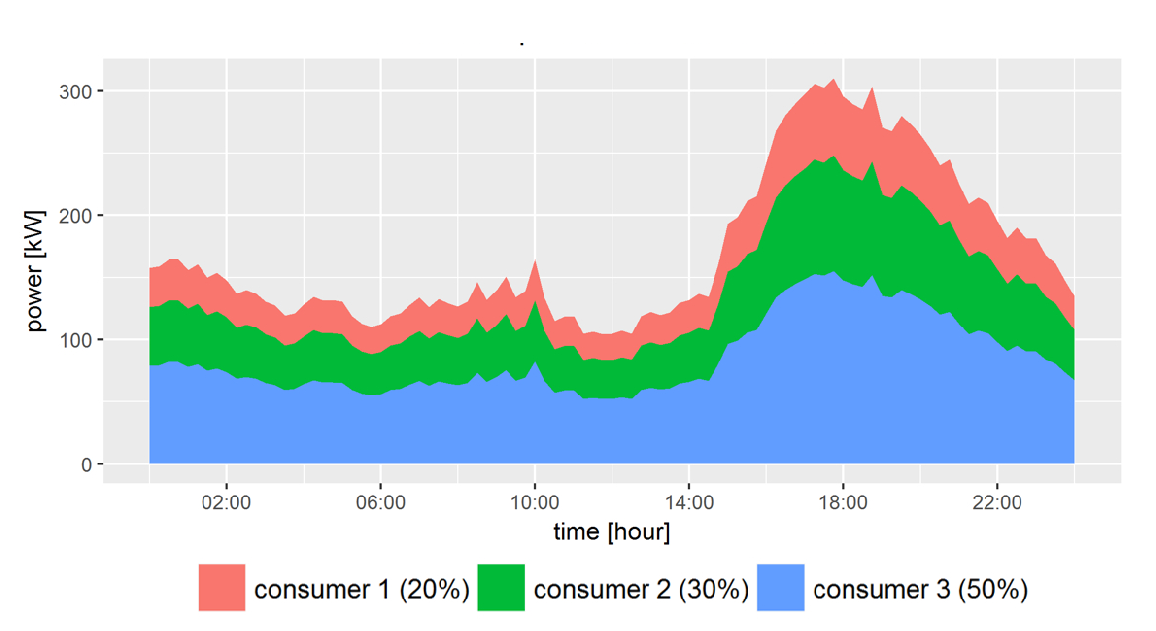
\includegraphics[ height=7.5cm, width=13cm]{figures/pseudo_measurements.pdf}
        \caption{Reference profile and load allocation}
        \label{fig:pseudo_scale}
    \end{figure}
,as for the pseudo active power injection of the bus, if there is no PV generator connected to the bus, the active power injection equals the pseudo active power consumption. Otherwise, the PV generation at that bus $p_{gen}^j$ should be added to the pseudo active power consumption to get the pseudo active power injection at bus $i$ as follows:
\begin{align}
    p_{psu}^{i} &= p_{psu-con}^{i}+p_{gen}^j
    \label{eq:pseu_inj}
\end{align}
By using the equations introduced above, the pseudo active power injections can be generated for buses without information on active power injection. The process for generating pseudo reactive power injection is similar to the pseudo active power injection generation except that there is no reactive power generation from PV generator. Because the aim of generating pseudo-measurements is to ensure the observability of the system and pseudo-measurements usually have a big mismatch to its real measured value, the standard deviation of the pseudo-measurements are set to be 0.3 p.u. which is substantially higher than the standard deviation from smart meters and virtual measurements which are set to 0.01. By using a Monta-Carlo simulation for selecting different meters locations, 100 cases are generated for each of the 30 scenarios. Figures \ref{fig:Pseudo Active Power Injection at Bus 2} and \ref{fig:Pseudo Active Power Injection at Bus 4} show two typical pseudo active power injections and its real active power injection.
    \begin{figure}[!h]
        \centering
        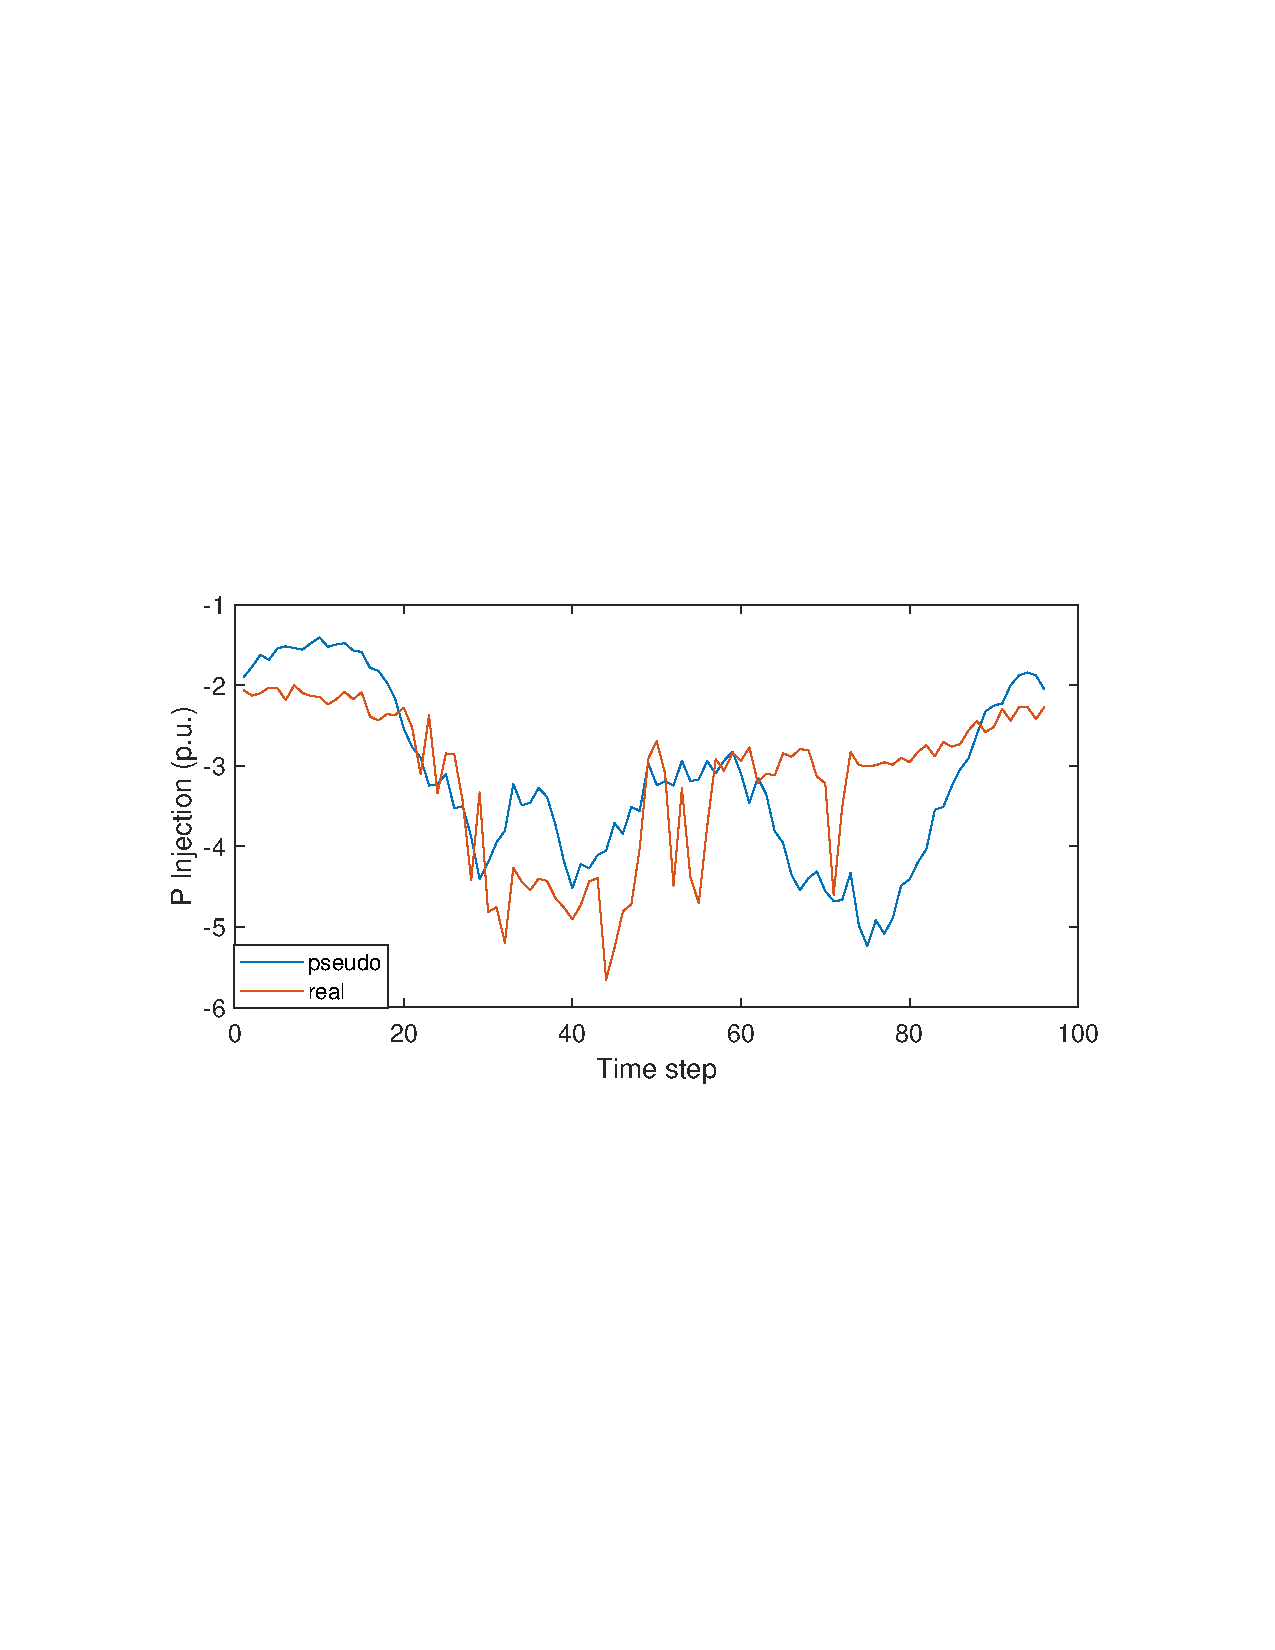
\includegraphics[ height=7cm, width=12cm]{figures/pseudo_P_1.pdf}
        \caption{Pseudo and actual active power injection}
        \label{fig:Pseudo Active Power Injection at Bus 2}
    \end{figure}
    
    \begin{figure}[!h]
        \centering
        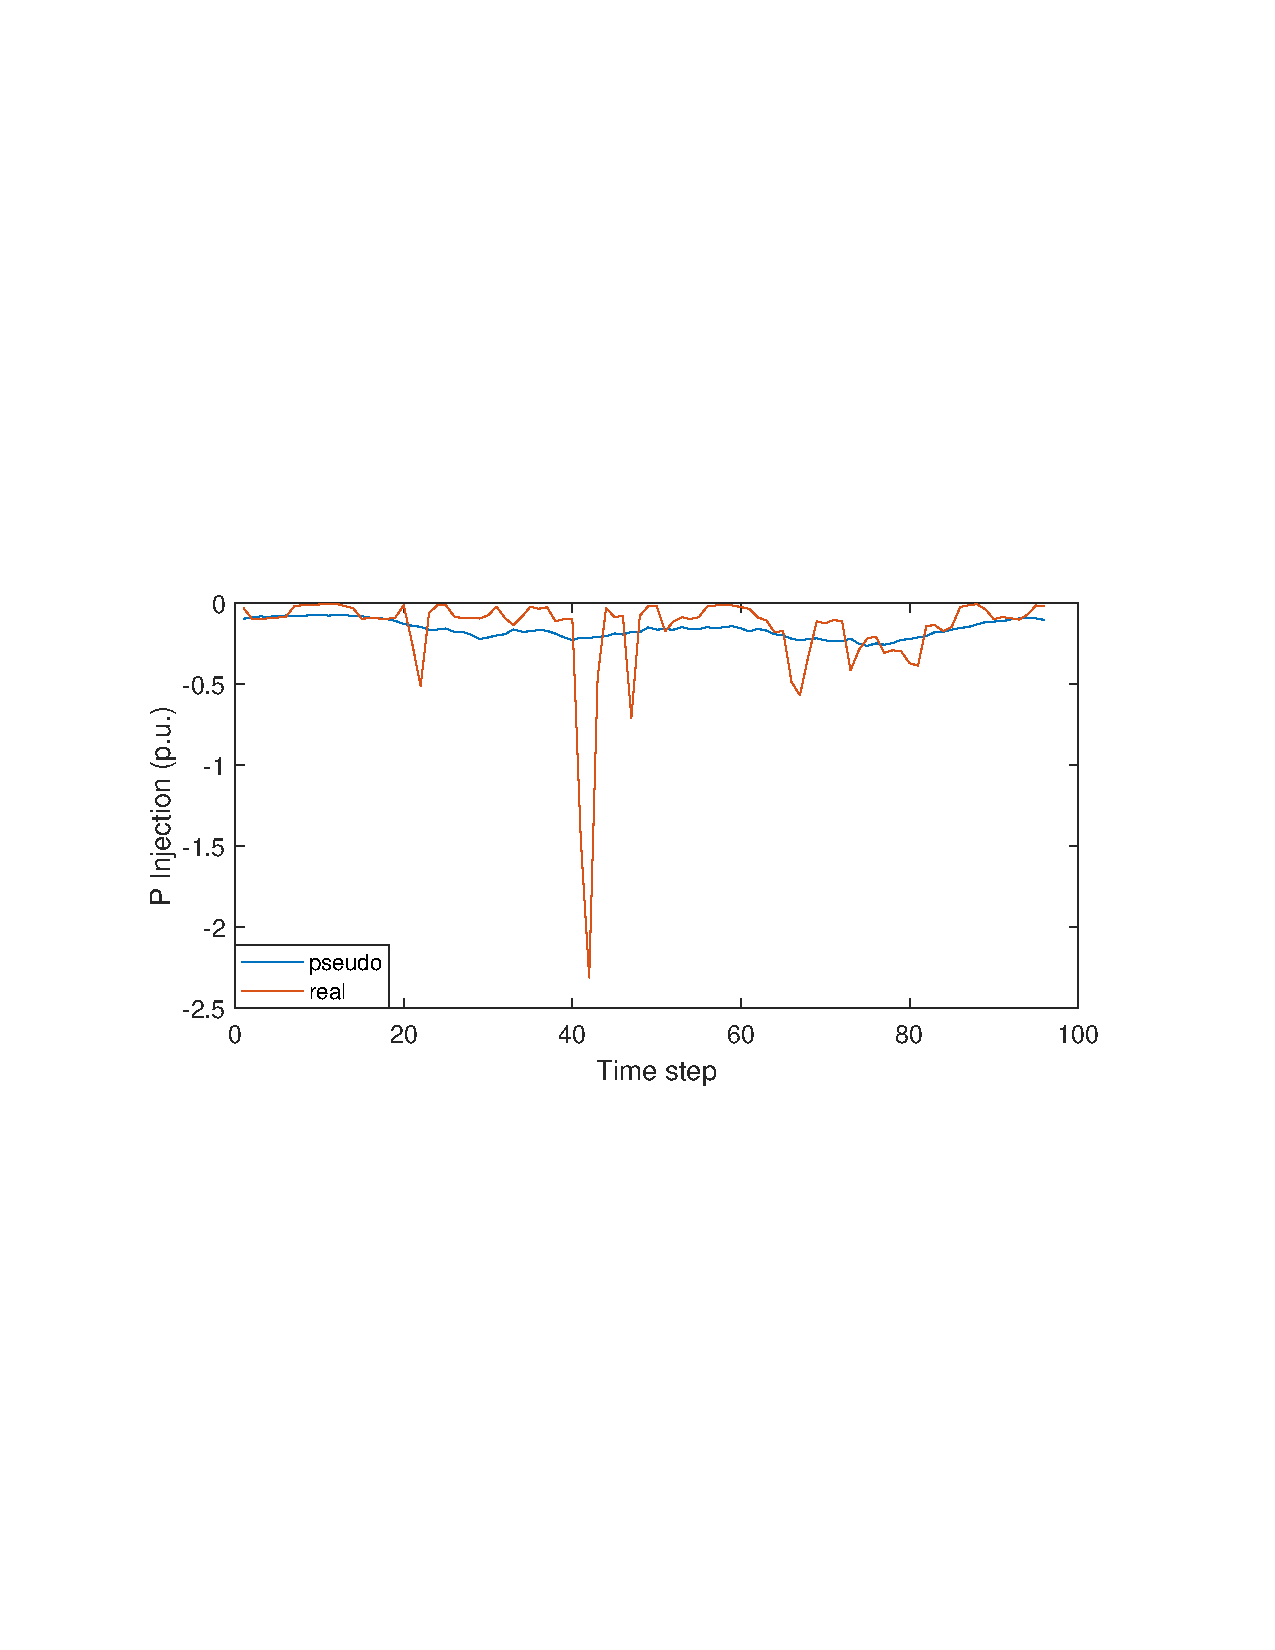
\includegraphics[ height=7cm, width=12cm]{figures/pseudo_P_2.pdf}
        \caption{Pseudo and actual active power injection} 
        \label{fig:Pseudo Active Power Injection at Bus 4}
    \end{figure}
\noindent
It can be seen that the pseudo active power injection follows the main trend of the real active power injection since the curve is relatively smooth, but the proposed pseudo-measurements generation method based on the total energy consumption can not match well when the load changes fast and sharply as shown in Figure \ref{fig:Pseudo Active Power Injection at Bus 4}, notably at time step 41, where there is a big mismatch between the pseudo measurement and its real value. However, despite the big mismatch at time step 41 in Figure \ref{fig:Pseudo Active Power Injection at Bus 4}, the overall absolute mismatch through all 96 time steps at bus 4 is smaller than the one in Figure \ref{fig:Pseudo Active Power Injection at Bus 2} due to the lower mean power level.
    \begin{figure}[!h]
        \centering
        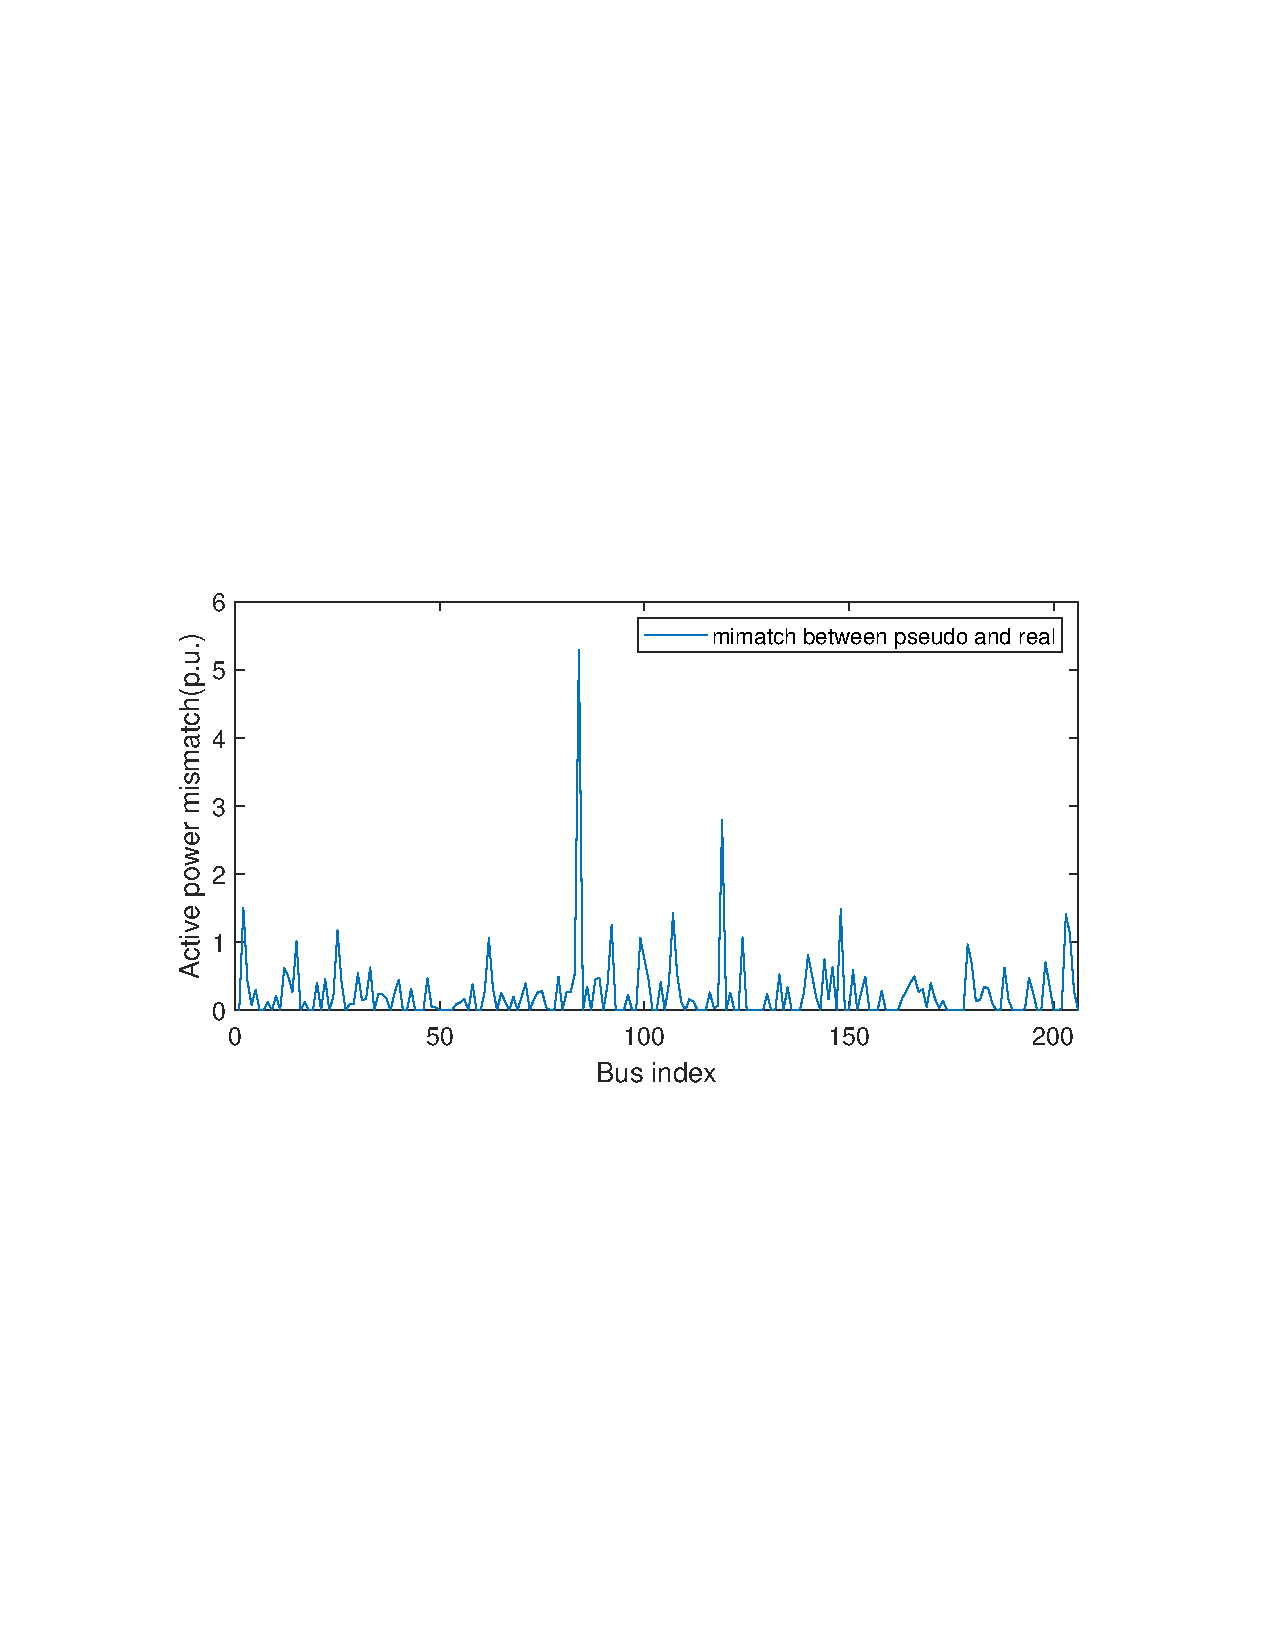
\includegraphics[ height=7cm, width=12cm]{figures/mismatch_psu_real.pdf}
        \caption{Total active power injection mismatch at each bus} 
        \label{fig:active power injection mismatch at each bus}
    \end{figure}
Even though the proposed pseudo-measurements generation method is based on the assumption that the total energy consumption at each node is known, there is still some total energy consumption mismatch between pseudo measurements and real measurement at the bus with a pseudo active power injection, as shown in Figure \ref{fig:active power injection mismatch at each bus}. The x-axis is the index of the 206 buses and the y-axis is the absolute mismatch between the real and pseudo measurements of 96 time steps. Notice that, obviously, there is no mismatch at with a real or virtual measurement. The reason why there is a mismatch at the pseudo measurement buses is that transmission losses are neglected in Equation \ref{eq:pseu_con}. As a result, the total active power consumption mismatch for all 206 buses depicted in Figure \ref{fig:active power injection mismatch at each bus} should be equal to the total active power losses during that day \cite{ghosh1997load}.
%4
\chapter{Simulation and Result Analysis}
\label{chap:Simulation_And_Result_Analysis}
This chapter shows and analyses the simulation results for four state estimation algorithms. Firstly, the performance over time is studied. Secondly, the influence of the location of the smart meters on the estimation accuracy is investigated and the optimal smart meters location is suggested. After that, the performance of the four estimators based on the proposed optimal smart meters location is compared to the cases with random smart meters location. Finally, the advantages and disadvantages of these four estimators are given.
\section{Performance Indices}
Before the result analysis, some performance indices are introduced in this section for determining the performance of the state estimation algorithms. 
\subsection{Absolute p.u. Error}
The most straightforward performance index is the absolute p.u. error between the estimated value and its real value without noise. All types of estimated measurements value can be obtained from the estimated state from the estimator together with the ideal measurement function $h_{ideal}(x)$. Compare to the measurement function $h(x)$ which calculates only the estimated value of the measurement from smart meters, $h_{ideal}(x)$ calculates the voltage magnitude, the power injection at all buses, and power flow on all branches of the system in p.u., which is shown below:
    \begin{align}
        h_{ideal}(x)=\begin{bmatrix}
                    V_e &
                    P_{inj-e} &
                    Q_{inj-e} &
                    P_{flow-e} &
                    Q_{flow-e} &
              \end{bmatrix}^\intercal
        \label{eq:ideal measurement jacobian  matrix}  
    \end{align}
, where $V_e$, $P_{inj-e}$ and $Q_{inj-e}$ represents the estimated voltage magnitude, active and reactive power injection at all buses in the system in p.u.. $P_{flow-e}$ and $Q_{flow-e}$ correspond to the active and reactive power flow over all branches in p.u..
The real value of the corresponding elements without noise in $h_{ideal}$ is called $z_{ideal}$, and the elements inside $z_{ideal}$ are shown in the equation below in p.u.:
    \begin{align}
        z_{ideal}=\begin{bmatrix}
                    V_{ideal} &
                    P_{ideal} &
                    Q_{ideal} &
                    P_{ideal} &
                    Q_{ideal} &
              \end{bmatrix}^\intercal
        \label{eq:ideal measurement}  
    \end{align}
Then, the absolute p.u. error can be calculated by using the estimated value $h_{ideal}$ minus its real value $z_{ideal}$. For example, the absolute voltage magnitude error $V_{error}^{i,t}$ of bus $i$ at time step $t$ in p.u. can be calculated as:
\begin{align}
    V_{error}^{i,t} &= |V_e^{i,t}-V_{ideal}^{i,t}|
    \label{eq:Verror}
\end{align}
All of the absolute p.u. errors are listed in Table \ref{tab:Error Types in p.u.}. The estimated and real value of the voltage phase angle is not included in $z_{ideal}$ or $h_{ideal}$.
    \begin{table}[!h]
        \centering
        \begin{tabular}{c|c|c}
            type of error & symbol & unit\\ \hline
            voltage magnitude & V_{error} & p.u. \\
            voltage phase angle & \theta_{error} & radian \\
            active power injection & P_{inj-error} & p.u. \\
            reactive power injection & Q_{inj-error} & p.u. \\
            active power flow & P_{flow-error} & p.u. \\
            reactive power flow & Q_{flow-error} & p.u. \\
        \end{tabular}
        \caption{Error Types in p.u.}
        \label{tab:Error Types in p.u.}
    \end{table}
\subsection{Ideal Cost}
The next performance index is a revised version of the cost function $J$ which can be called ideal cost function $J_{ideal}$ and calculated as follows:
\begin{align}
    J_{ideal}^t(x^t) &= (h_{ideal}(x^t)-z_{ideal}^t)^{\intercal} (h_{ideal}(x^t)-z_{ideal}^t)
    \label{eq:J_ideal}
\end{align}
, where $J_{ideal}^t(x^t)$ is the ideal cost under the state $x^t$ at time step t. Because there are totally 96 time steps in each case, then $t$ is ranging between 1 to 96 in this thesis. Compared to the cost function $J$, the ideal cost $J_{ideal}$ considering all error between estimated value and real value whereas cost $J$ only considering the error between estimated value and its corresponding measurement from smart meters with noise. 

\subsection{Root Mean Squared Error}
Root Mean Squared Error (RMSE) calculates the quadratic mean error between the prediction value and observed value over a certain time series. Because there is a square on the error ahead of the mean, RMSE is more sensitive to large error. In this project, the RMSE for each measurement in $z_{ideal}$ is calculated as follows:
\begin{align}
    RMSE &= \sqrt{ \frac{ \sum_{t=1}^{T} (\hat{y}^t-y^t) ^2}{T}}
    \label{eq:RMSE}
\end{align}
, where $\hat{y}^t$ is the predicted value at time step $t$ which can be replaced by the elements in $h_{ideal}(x^t)$ and $y^t$ is the real value which can be replaced by the corresponding value in $z^t_{ideal}$.

\subsection{Pearson Correlation Coefficient}
The Pearson correlation factor is a statistic factor which detects the linear relation between two variables and is denoted by $r$. The Pearson correlation factor takes values between -1 and 1. When $r$ is zero, it means that there is no correlation between these two variables. Negative $r$ indicates a negative correlation and a positive value means that there is a positive correlation between the two variables. The closer the absolute value of $r$ to 1, the stronger linear relation they have as shown in Figure \ref{fig:pearson_factor}:
    \begin{figure}[!h]
        \centering
        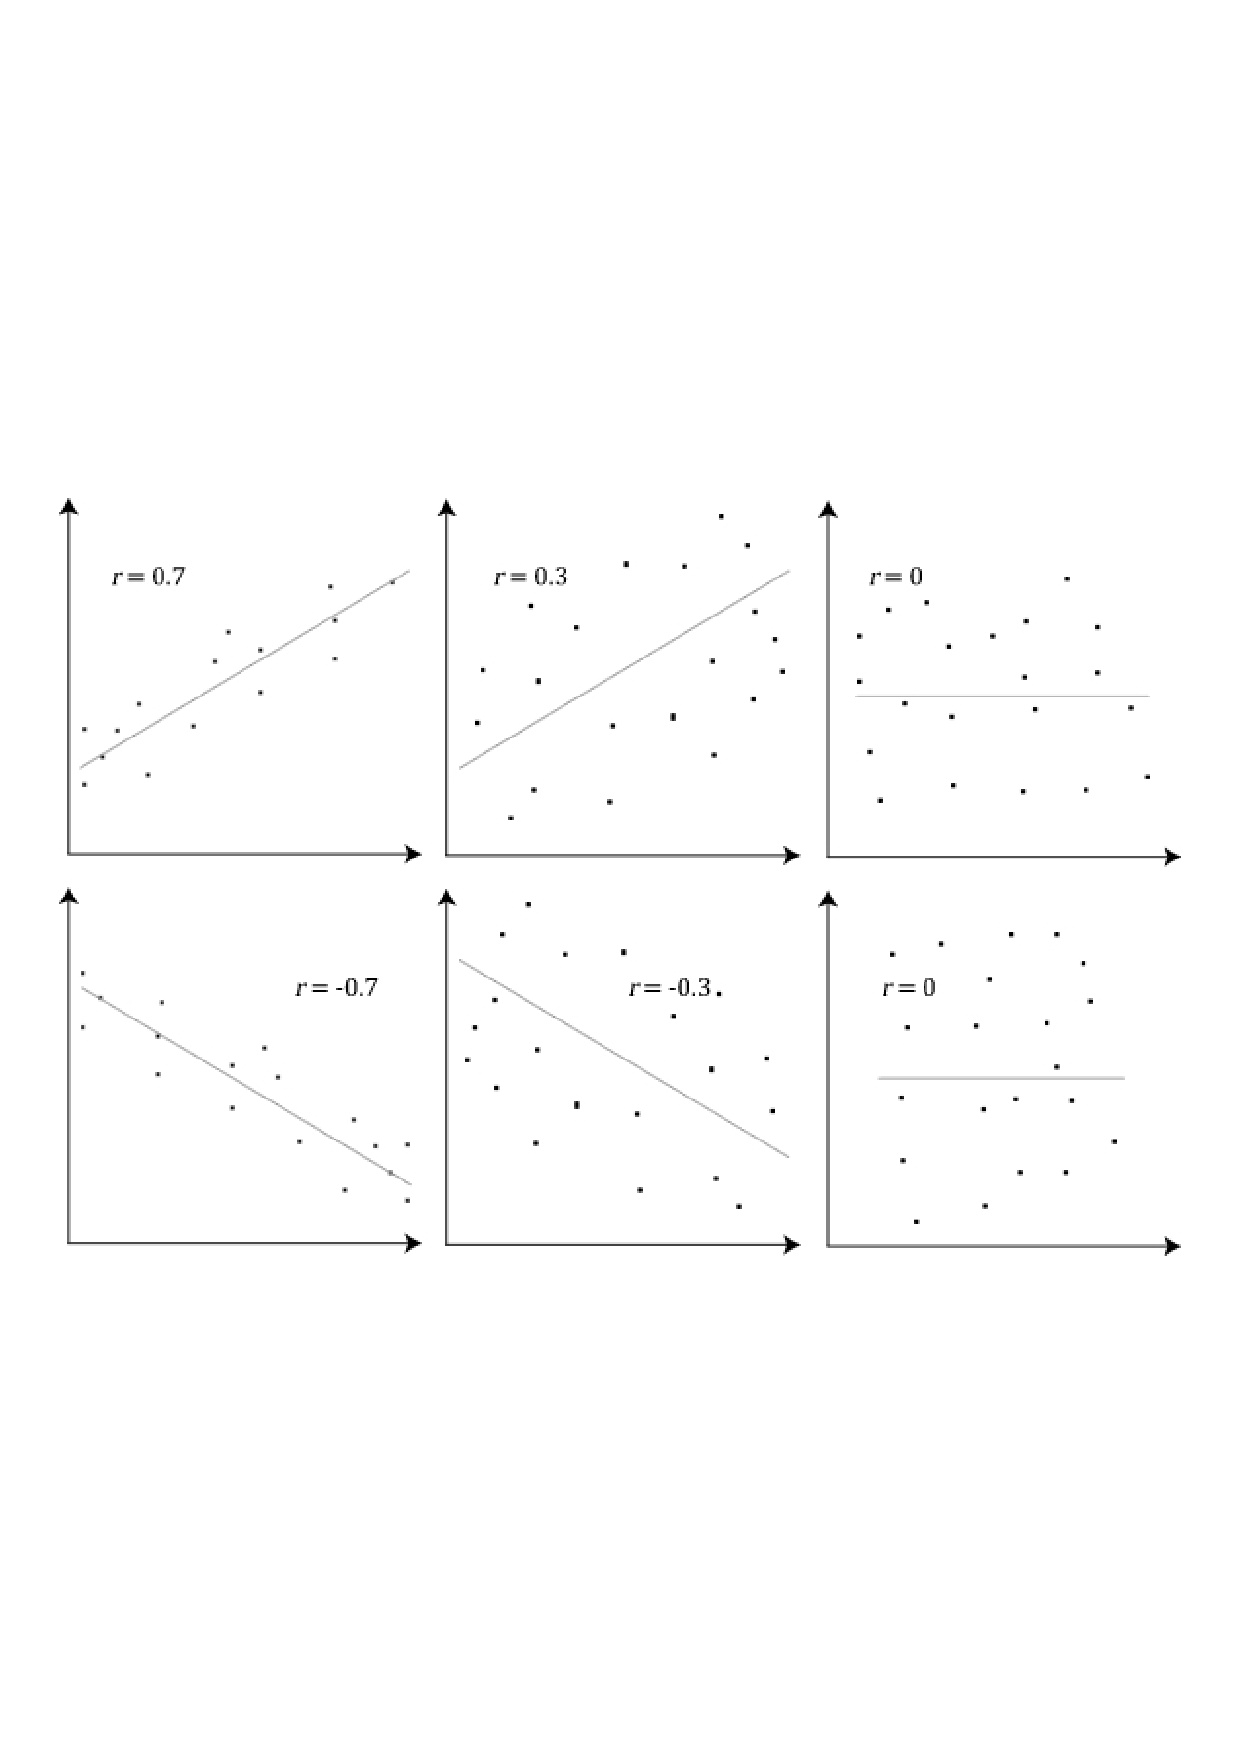
\includegraphics[ height=7cm, width=12cm]{figures/pearson.pdf}
        \caption{Different levels of Pearson correlation factor between two variables \cite{standard}}
        \label{fig:pearson_factor}
    \end{figure}
    
\noindent
The Pearson correlation coefficient $r$ between $X=[x_1,x_2,\cdots,x_n]$ and $Y=[y_1,y_2,\cdots,y_n]$ can be calculated by the equation below:
\begin{align}
    r &= \frac{\sum_{i=1}^{n}(x_i-\bar{x})(y_i-\bar{y})}{\sqrt{\sum_{i=1}^{n}(x_i-\bar{x})^2}\sqrt{\sum_{i=1}^{n}(y_i-\bar{y})^2}}
    \label{eq:pearson}
\end{align}
, where $\bar{x}$ is the mean value of $X$ and $\bar{y}$ is the mean value of $Y$. 

\subsection{Spearman Rank Correlation Coefficient}
\label{sect:spearman}
Spearman's rank correlation coefficient is used for detecting the positive or negative trend relation between two variables. Different from the Pearson correlation coefficient, the Spearman rank correlation coefficient does not require a constantly increasing or decreasing rate. The Spearman coefficient is close to 1 or -1 as long as the tested two variables are changing monotonically. So, the Spearman correlation coefficient can be understood as a Pearson correlated coefficient of ranked variables which gives the respondent a set of items and asks them to put the items in some form of order. Figure \ref{fig:spearman_factor} shows a clear view of the comparison between Pearson and Spearman correlation coefficients under different situations. 
    \begin{figure}[!h]
        \centering
        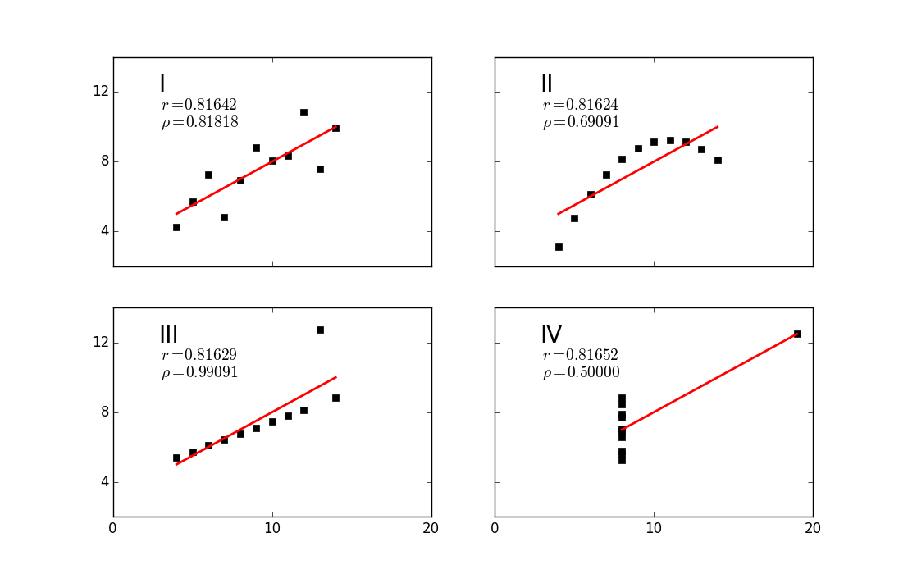
\includegraphics[ height=7cm, width=12cm]{figures/spearman.pdf}
        \caption{Comparison between Spearman and Pearson coefficient\cite{spearman}}
        \label{fig:spearman_factor}
    \end{figure}
By knowing the rank order of two variables, the Spearman correlated coefficient $\rho$ can be calculated as:
\begin{align}
    \rho &= 1- \frac{6 \sum_{i=1}^{n}d_i^2}{n(n^2-1)}
    \label{eq:spearman factor}
\end{align}
, where $d_i$ is the rank order difference at the $i^{th}$ observation and $n$ is the total number of observations. Because the Spearman correlation coefficient shows the rank order correlation, this factor is mainly used for detecting the influence of smart meters location on the accuracy of estimators, because the Pearson correlation coefficient shows the linear relationship between two variables whereas the trend of the correlation is more interested. Also, the index, which represents the smart meters distribution or distance, only shows the overall tendency of the smart meters location which makes Spearman correlation coefficient a more suitable index than Pearson correlation coefficient. 

\subsection{Standards for Correlation Coefficients}
\label{sect:threshold_0.3}
After obtaining the value of the correlation coefficients, it is necessary to build standards for determining the strength of the correlation between variables. Table \ref{tab:Correlation coefficient strength} shows a rough standard for determining the strength of the correlation factor. In this project, 0.3 is selected to be the threshold above which two variables are correlated.
    \begin{table}[!h]
        \centering
        \begin{tabular}{c|c}
            Absolute value & strengh\\ \hline
            .00 $\sim$ .19 &  $very \, weak(vw)$   \\
            .20 $\sim$ .39 &  $weak(w)$ \\
            .40 $\sim$ .59 & $moderate(m)$ \\
            .60 $\sim$ .79 & $strong(s)$ \\
            .80 $\sim$ 1.0 & $very \, strong(vs)$ \\
        \end{tabular}
        \caption{Correlation coefficient strength \cite{spearman_strength}}
        \label{tab:Correlation coefficient strength}
    \end{table}


\section{Result Analysis Over Time}
This section focuses on analyzing the error of the four estimators over time. For each scenario with different levels of measurements, there are 100 cases with different random location of smart meters. For each case, there are 96 time steps, which represents one day. After running the state estimation on 30 scenarios, the ideal cost $J_{ideal}^t$ is calculated by Equation \ref{eq:J_ideal} for each time step in each of the 100 cases and in each scenario. After that, the outliers of $J_{ideal}^t$ within 96 time steps in each case should be detected by using the 'isoutlier' function in MATLAB. The function 'isoutlier' calculates the median value of $J_{ideal}^t$ over the 96 time steps and the outliers in this function are defined as the value which is more than three scaled Median Absolute Deviations ($MADs$) the median value. For time series $X=[x_1,x_2,\cdots,x_n]$, the $MAD$ value can be derived as:
\begin{align}
    MAD &= med(|x_i-med(X)|)
    \label{eq:MAD}
\end{align}
, where $med$ means the median value of an array. In this case, only the values which exceed the upper threshold are defined as outliers, as shown in Figure \ref{fig:J ideal outlier}.
    \begin{figure}[!h]
        \centering
        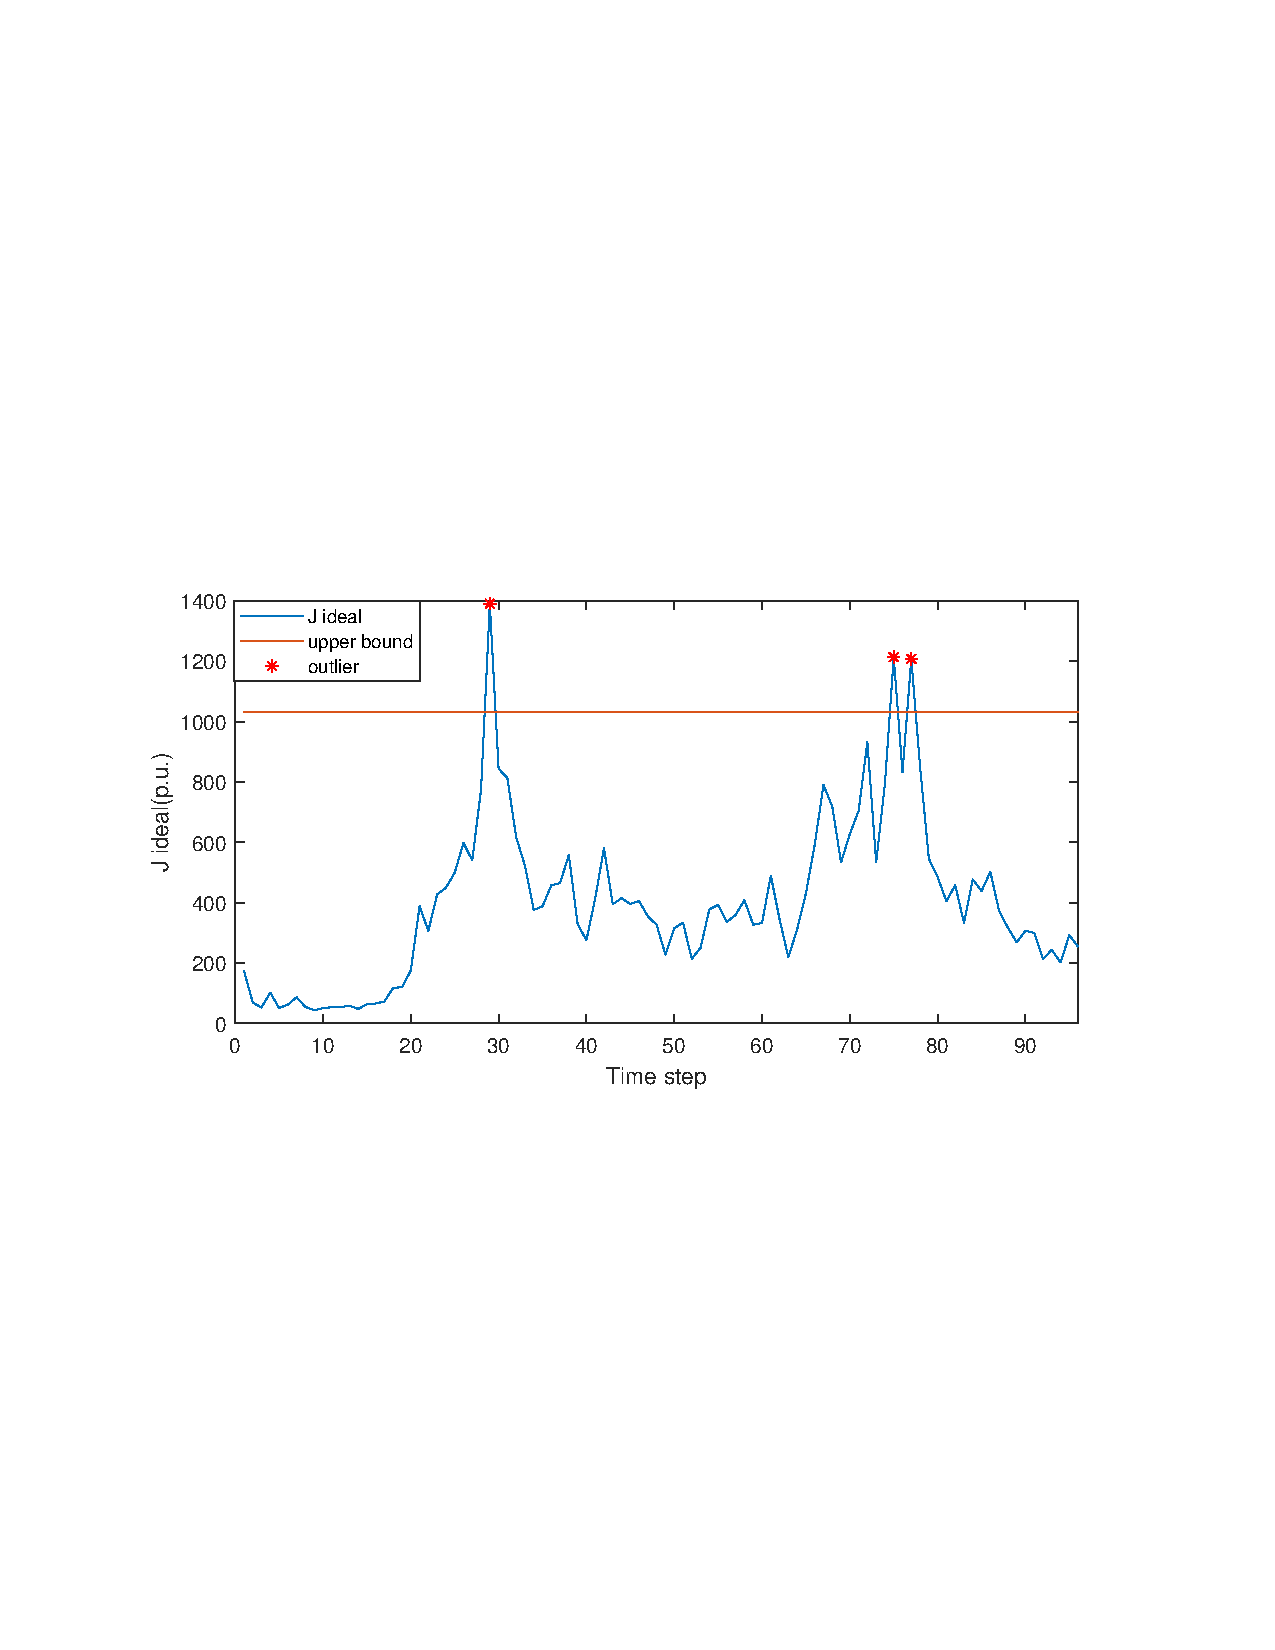
\includegraphics[ height=7cm, width=12cm]{figures/J_ideal_outlier.pdf}
        \caption{J ideal outlier detection}
        \label{fig:J ideal outlier}
    \end{figure}
\bigskip
\\Table 4.3 summarizes the proportion of the error in voltage magnitude, active and reactive power injection, and active and reactive power flows in scenario 9. It comes out that the active power flows are responsible for a large portion of the error (i.e., $91 \%$ in scenario 9).
    \begin{table}[!h]
        \centering
        \begin{tabular}{c|c}
            type of error & proportion\\ \hline
            V_{error} &  {< 1 \%}   \\
            P_{inj-error} &  4 \% \\
            Q_{inj-error} & {< 1 \%} \\
            P_{flow-error} & 91 \% \\
            Q_{flow-error} & 4 \% \\
        \end{tabular}
        \caption{Proportion of each type of error in scenario 9}
        \label{tab:pie table}
    \end{table}
 The reason that the contribution from reactive power flow is smaller than that from active power flow is mainly because of the small constant power factor 0.98, and the reactive power consumption of each load is also relatively small compared with the active power consumption. Also, the number of branch power flow measurements is much higher than the other measurements due to the fact that there are two branch flow measurements (i.e., in both directions).
\bigskip
\\By knowing that most of the $J_{ideal}$ outliers are due to the high active power flow mismatch between the estimated value and real value, the next step is to find the reason of high active power flow mismatch at those time steps. Firstly, the number of times for $J_{ideal}$ to be an outlier at one time step in 100 cases for each scenario is figured out. Secondly, the next goal is to identify at which time step $J_{ideal}$ tends to be an outlier. 
\bigskip
\\Figure \ref{fig:outlier number} shows an example of the total number of outlier $J_{ideal}$ at each time step across 100 cases in scenario 9. The left y-axis is the number of outlier $J_{ideal}$ and the right y-axis shows the sum of the squared active power flow mismatchs between the real value without noise and the estimated value from WLS for 100 cases in scenario 9. As shown in table \ref{tab:pie table}, a large proportion of $J_{ideal}$ comes from the active power flow. Notice, notably, the correlation between the number of outlier $J_ideal$ per time step and the squared active power flow mismatch.
    \begin{figure}[!h]
        \centering
        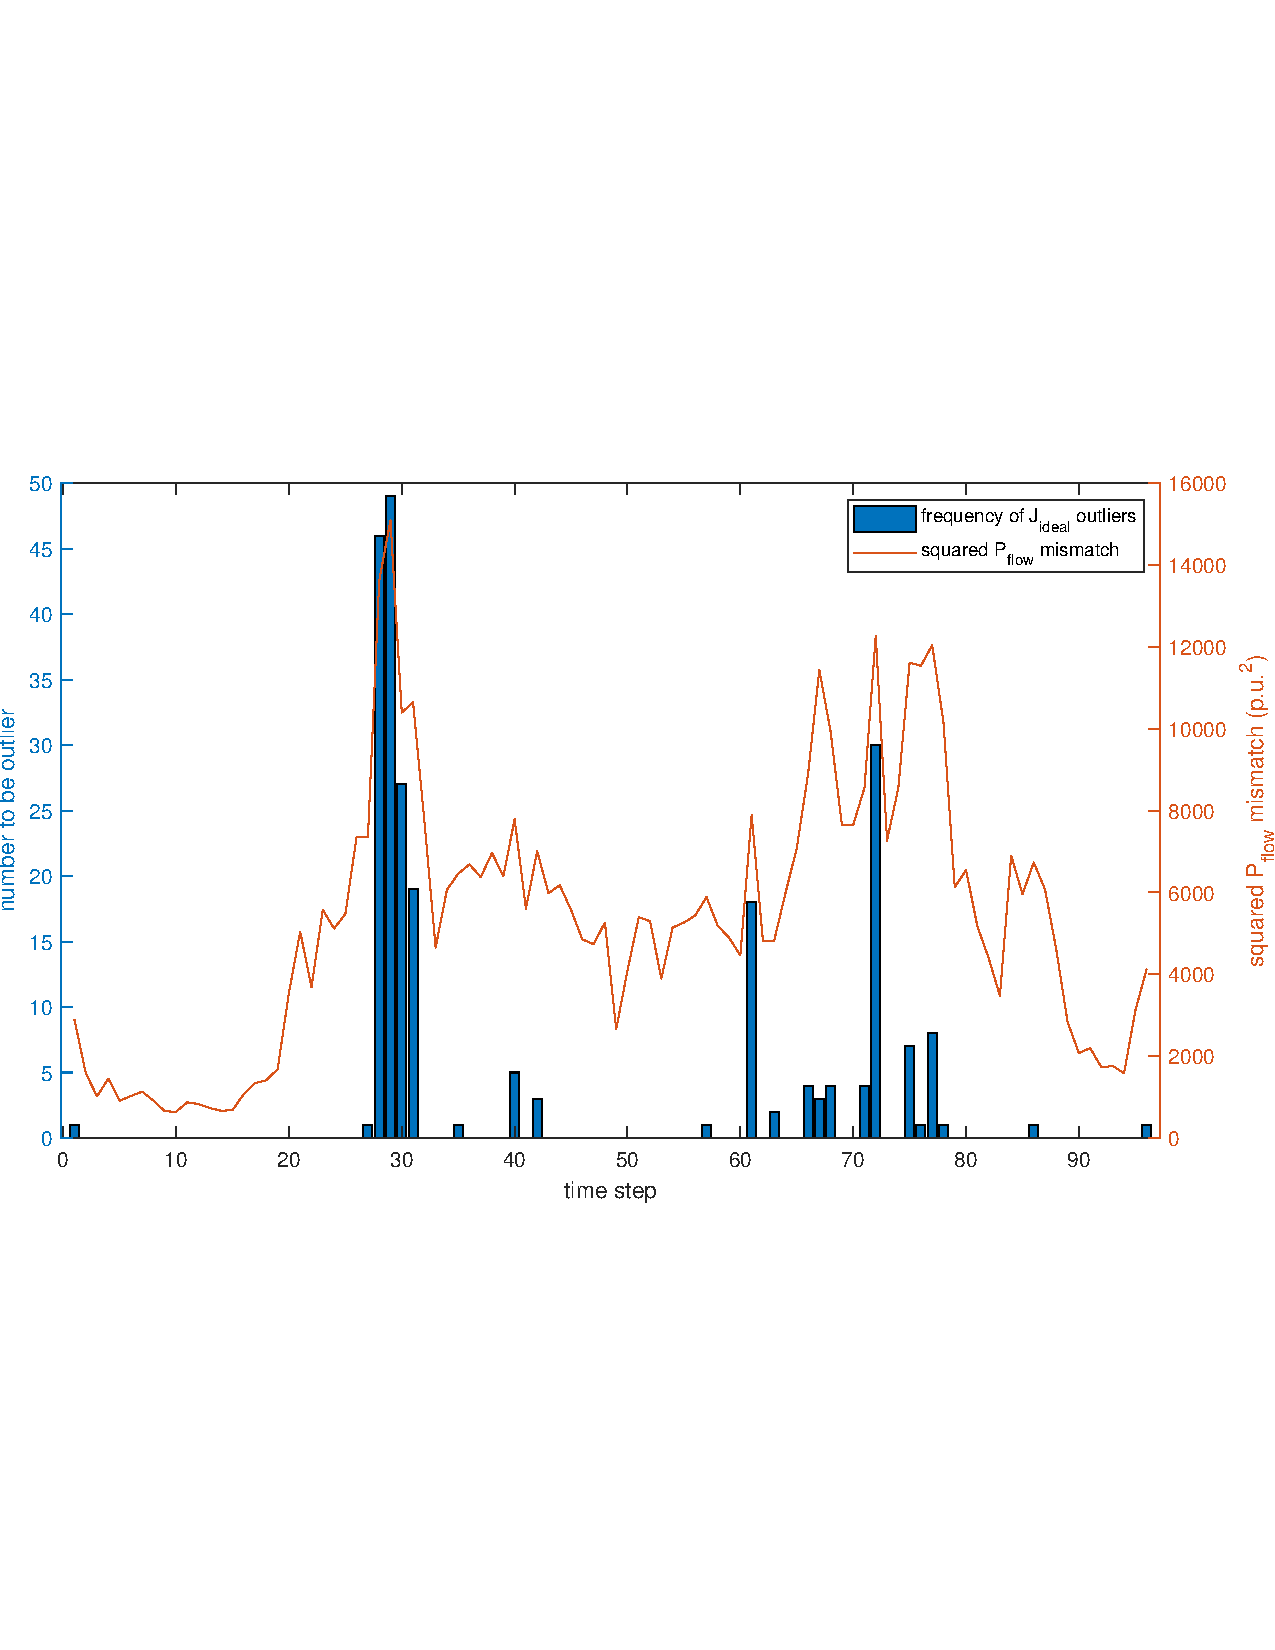
\includegraphics[ height=9cm, width=14cm]{figures/outlier.pdf}
        \caption{Frequency of $J_{ideal}$ outliers together with the squared $P_{flow}$ mismatch across one day}
        \label{fig:outlier number}
    \end{figure}
The total active power injection at those time steps where $J_{ideal}$ is high is due to houseloads daily activities, which increases the power consumption and thus the active power flow at those time steps. As the pseudo-measurement generation method can not predict the active power injection well when the active power injection is relatively high and spiky, the mismatch between pseudo active power injection and its real value is large, which leads to high active power flow mismatch. To prove this assumption, the Pearson's correlation coefficient factor between the number of $J_{ideal}$ outliers and the mean value of the sum active power injection mismatch at each time step among the 100 cases is calculated for each of the 30 scenarios.The result for WLS is shown in Figure \ref{fig:pearson_J_ideal_30_scenario}. Notice that similar results are obtained with the other algorithms.
\bigskip
\\In the Figure \ref{fig:pearson_J_ideal_30_scenario}, the bottom x-axis shows the index of 30 scenarios and the top x-axis shows the measurements level for bus meters.
\begin{figure}[!h]
        \centering
        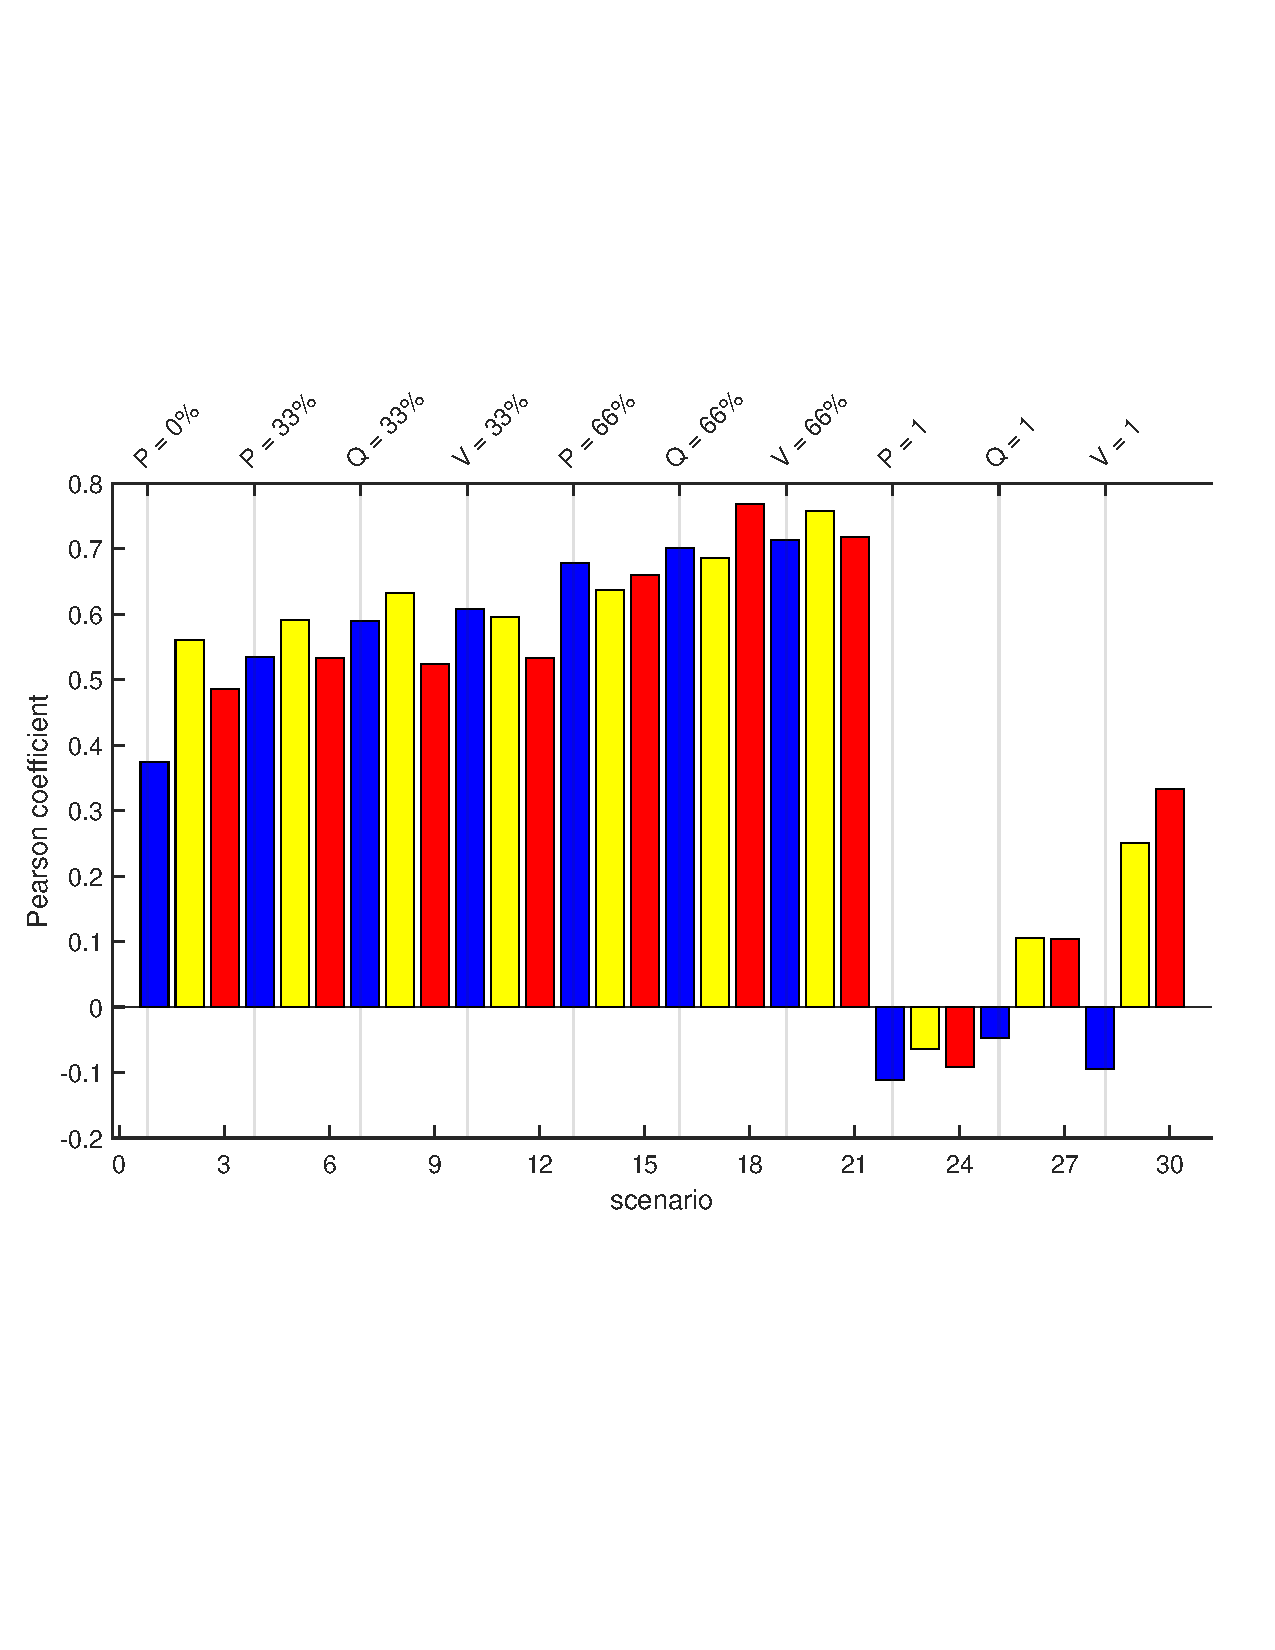
\includegraphics[ height=9cm, width=14cm]{figures/Pearson_J_ideal_outlier_WLS_bar.pdf}
        \caption{Pearson coefficient of active power injection mismatch and number of $J_{ideal}$ outliers for 30 scenarios}
        \label{fig:pearson_J_ideal_30_scenario}
\end{figure}
 For example, scenarios 3 to 5 represent the cases where $33\% $ of the buses have information of active power injection only, except the virtual measurements. And the blue, yellow and red bars correspond to the percentage of measured power flows, which are $0 \%$, $10 \%$, and $20 \%$, respectively. Except the case with $100 \%$ knowledge at buses, the correlation is relatively high and increases with the level of measurement penetration. However, scenarios 22 to 30 show a low correlation. This is mainly because there is no pseudo-measurements for active power injection anymore in these scenarios since the percentage of the buses which have information of active power injection is $ 100\% $ as shown in Table \ref{tab:30_scenarios}. Scenario 29 and 30 have a high Pearson factor compared with the other scenarios from 22 to 28 which does not fit the assumption that the active power injection mismatch does not have an influence on $J_{ideal}$ when the strong information of active power injection of all buses are known.
    \begin{figure}[!h]
        \centering
        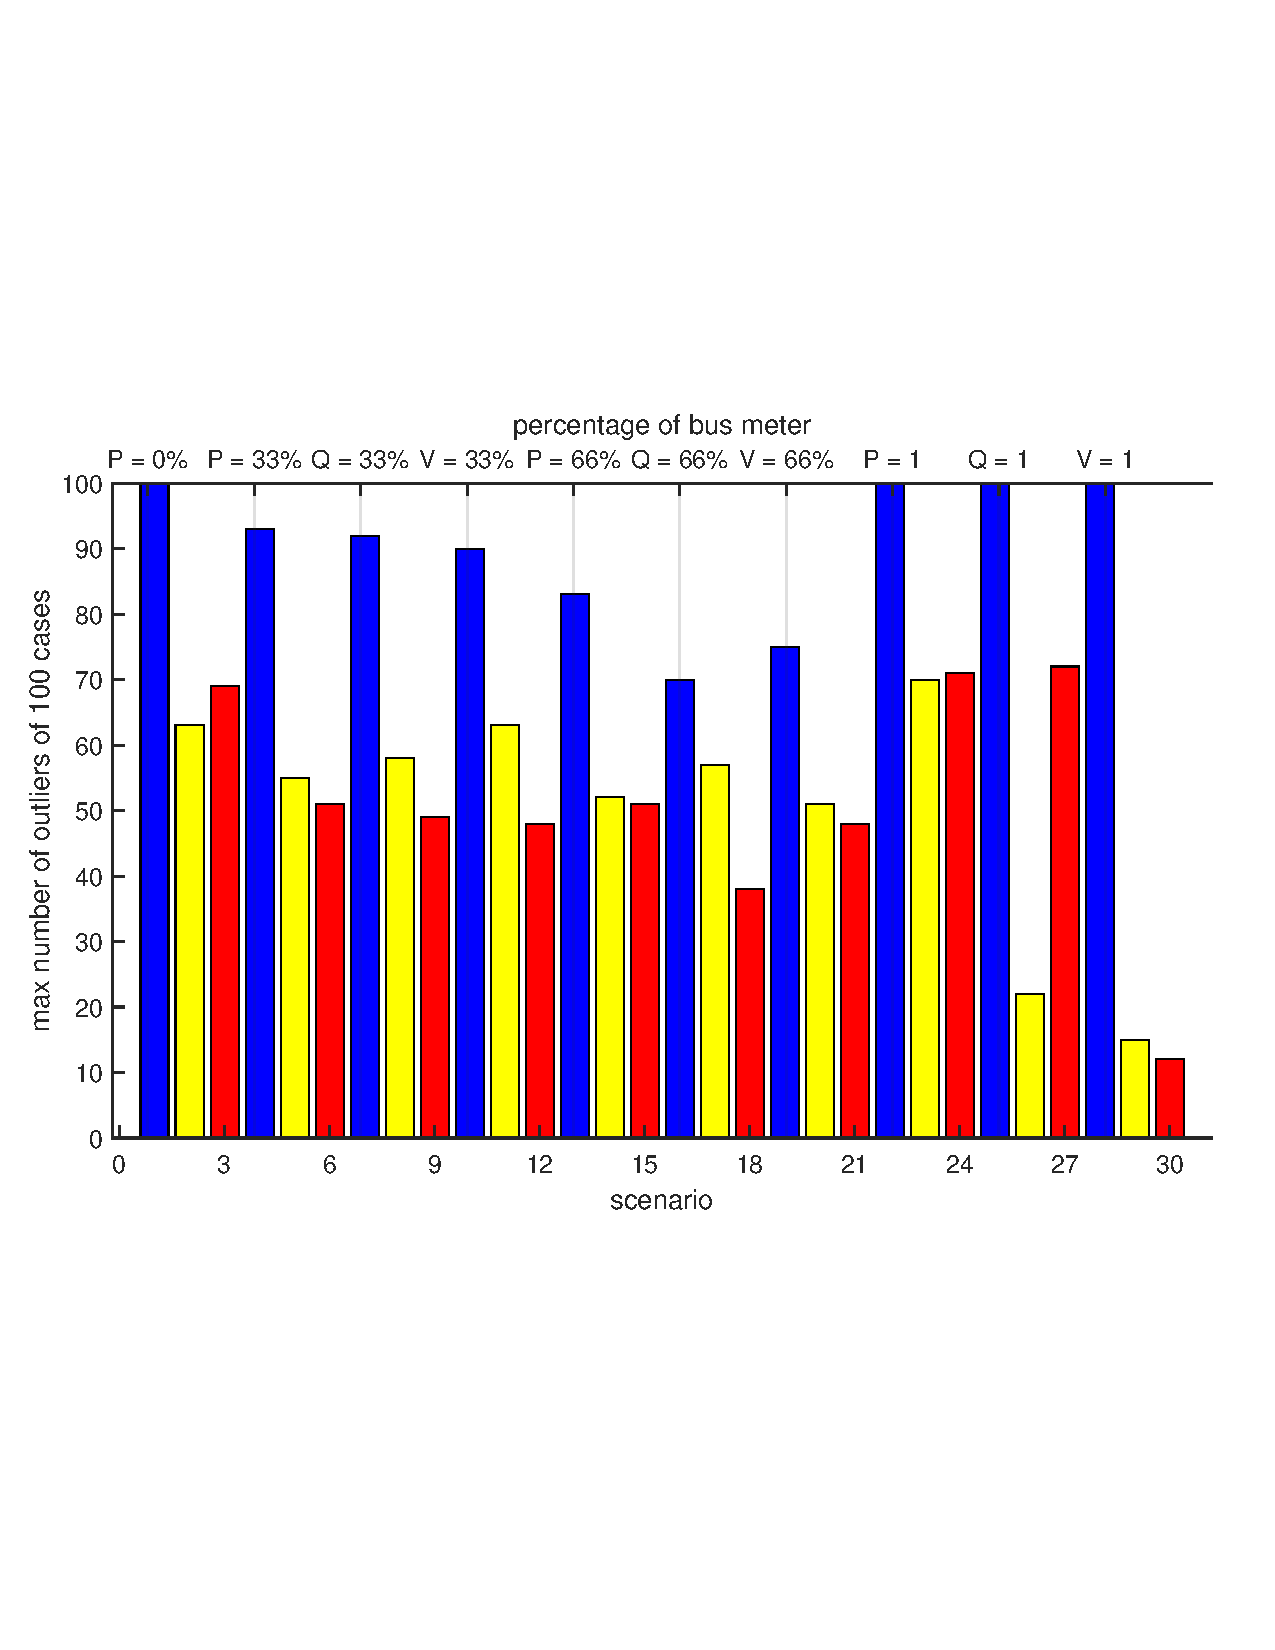
\includegraphics[ height=7cm, width=12cm]{figures/max_num_of_times_J_ideal_outlier.pdf}
        \caption{Max $J_{ideal}$ outlier for each scenario}
        \label{fig:max_num_of_times_J_ideal_outlier}
    \end{figure}
The reason is mainly because the maximum number of times for $J_{ideal}$ to be an outlier across 96 time steps are relatively small in scenarios 29 and 30, as shown in Figure \ref{fig:max_num_of_times_J_ideal_outlier}.
\bigskip
\\In conclusion, a high mismatch between pseudo and real active power injection measurements leads to a high error on active power flows, which is the most important factor in $J_{ideal}$ as indicated in Table \ref{tab:pie table}. By neglecting the first three scenarios where all of the active power injections are pseudo measurements and last 9 scenarios where all of the buses have meters for measuring active power injection, the mean Pearson correlation coefficient between the active power injection mismatch and the number of $J_{ideal}$ outliers is shown in Table \ref{tab:pearson_J_ideal} four the four estimators. It can be seen that the mean value of the coefficients are close to 0.6 which show a moderately strong relationship between these two variables.
    \begin{table}[!h]
        \centering
        \begin{tabular}{c|c|c|c|c}
             & WLS & EKF & SHGM & SVR-EKF\\ \hline
            $r(num_{J_{ideal}},P_{mis-inj})$ & 0.6358($s$) & 0.6058($s$) & 0.6279($s$) &  0.5942($m$)\\
        \end{tabular}
        \caption{Mean Pearson coefficient of active power injection mismatch and number of $J_{ideal}$ outliers}
        \label{tab:pearson_J_ideal}
    \end{table}
    


\section{Influence of Smart Meter Location}
\label{sec:analysis_meter_location}
The section investigates the influence of smart meter location on the accuracy of the estimators. The bus meters are the smart meters measuring the voltage magnitude, active power injection, and reactive power injection. The branch meters are sensors measuring active and reactive power flows on the branches. With a given number of bus meters and branch meters, the accuracy of the estimation results is different according to their location. To simplify the problem, the interaction between the bus meters and branch meters is neglected, which means that the influence of the bus and branch meters location on the estimator accuracy is considered independently. 
\subsection{Hierarchy of Bus and Branch}
This section introduces a method for classifying the buses and branches in the radial network into different hierarchies based on the distance from the bus or branch meters to the feeder bus or branch. 
\bigskip
\\The radial network has a tree structure without closed loop.
    \begin{figure}[!h]
        \centering
        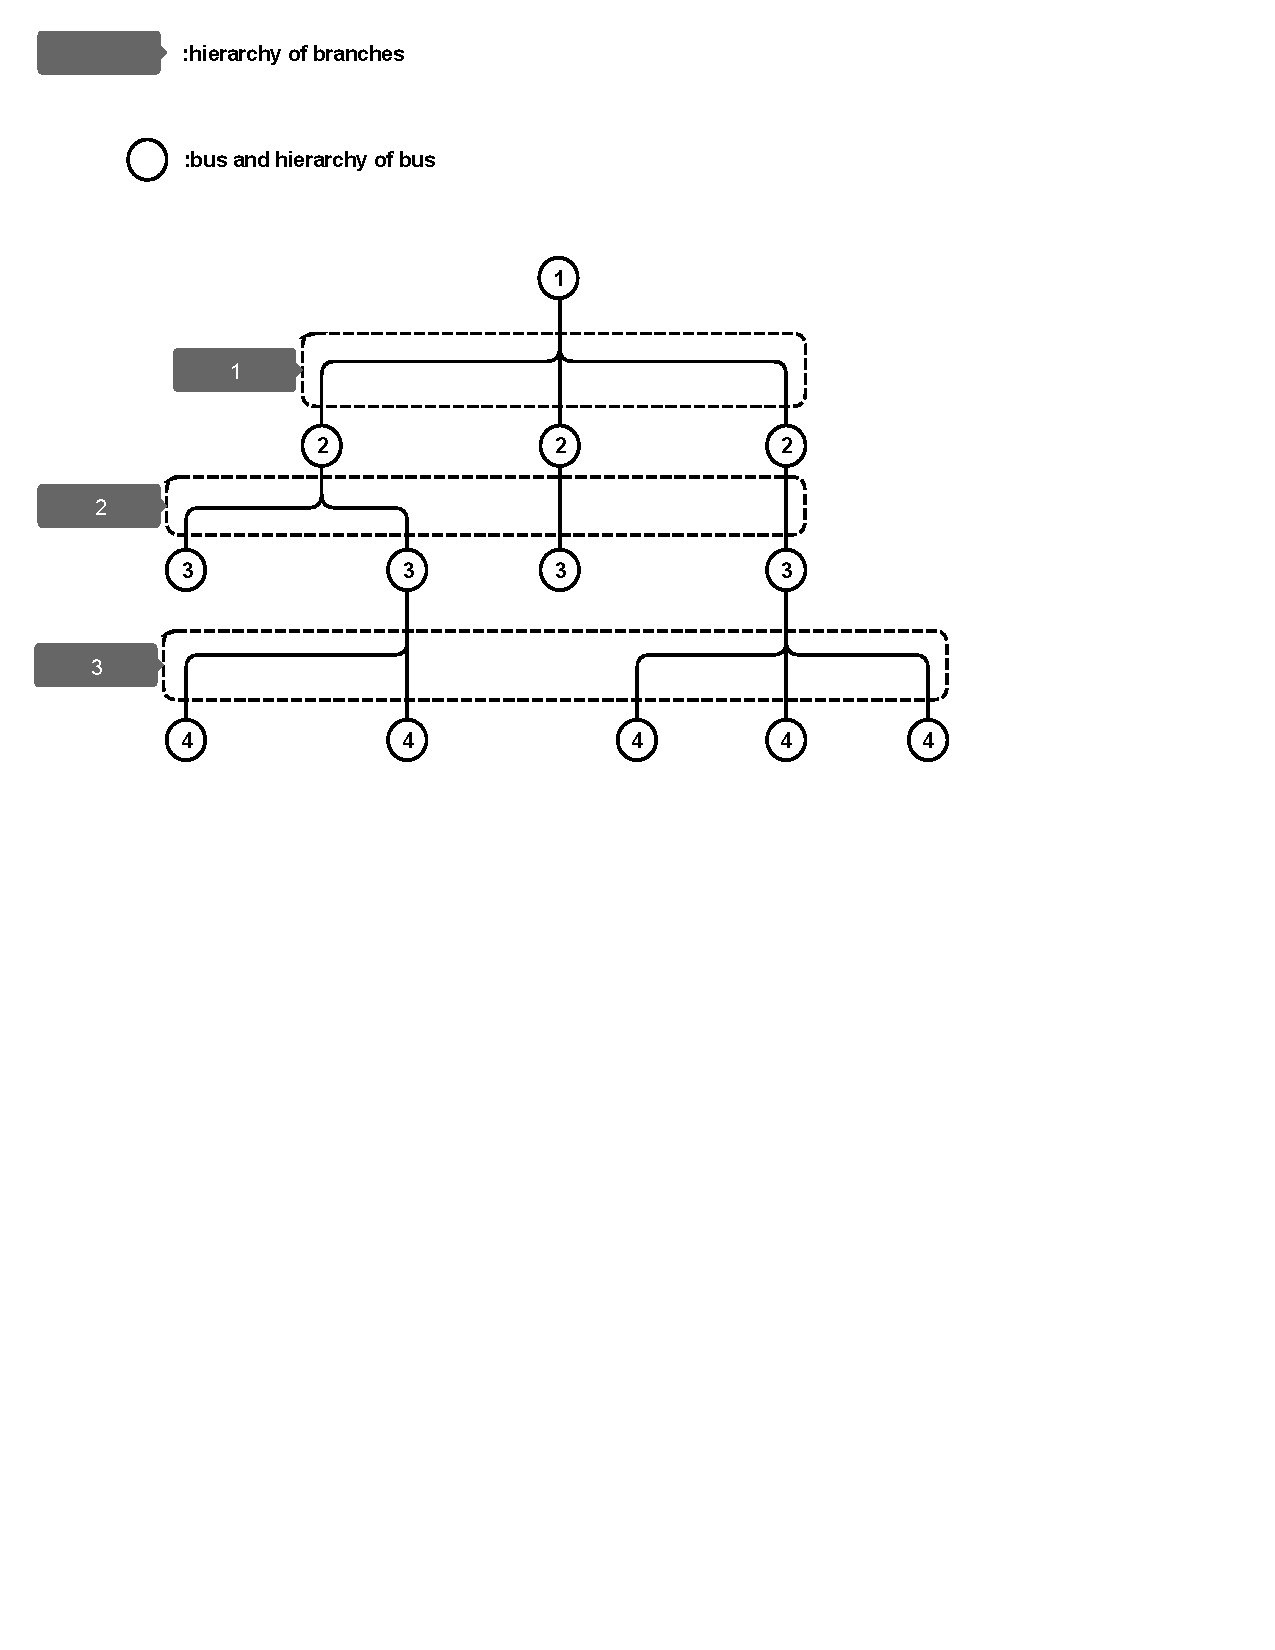
\includegraphics[ height=10cm, width=13cm]{figures/raidal_network_hierarchy.pdf}
        \caption{Hierarchy of buses and branches}
        \label{fig:radial hierarchy}
    \end{figure}
Figure \ref{fig:radial hierarchy} shows a simplified radial distribution grid with 13 buses, including the feeder bus at the top which is marked with 1. The hierarchy of a bus is defined as the distance from that bus to the feeder bus by assuming that the distance between two connected buses is one. In Figure \ref{fig:radial hierarchy} there are totally 4 layers in the bus hierarchy. The hierarchy of the feeder bus is defined as 1 and the hierarchy of the buses connected with feeder bus is 2, and so on. Since there is no closed loop, the distance between two buses, connected to a common upper hierarchy bus, is 2 as shown in Figure \ref{fig:distance_two_buses}.
    \begin{figure}[!h]
        \centering
        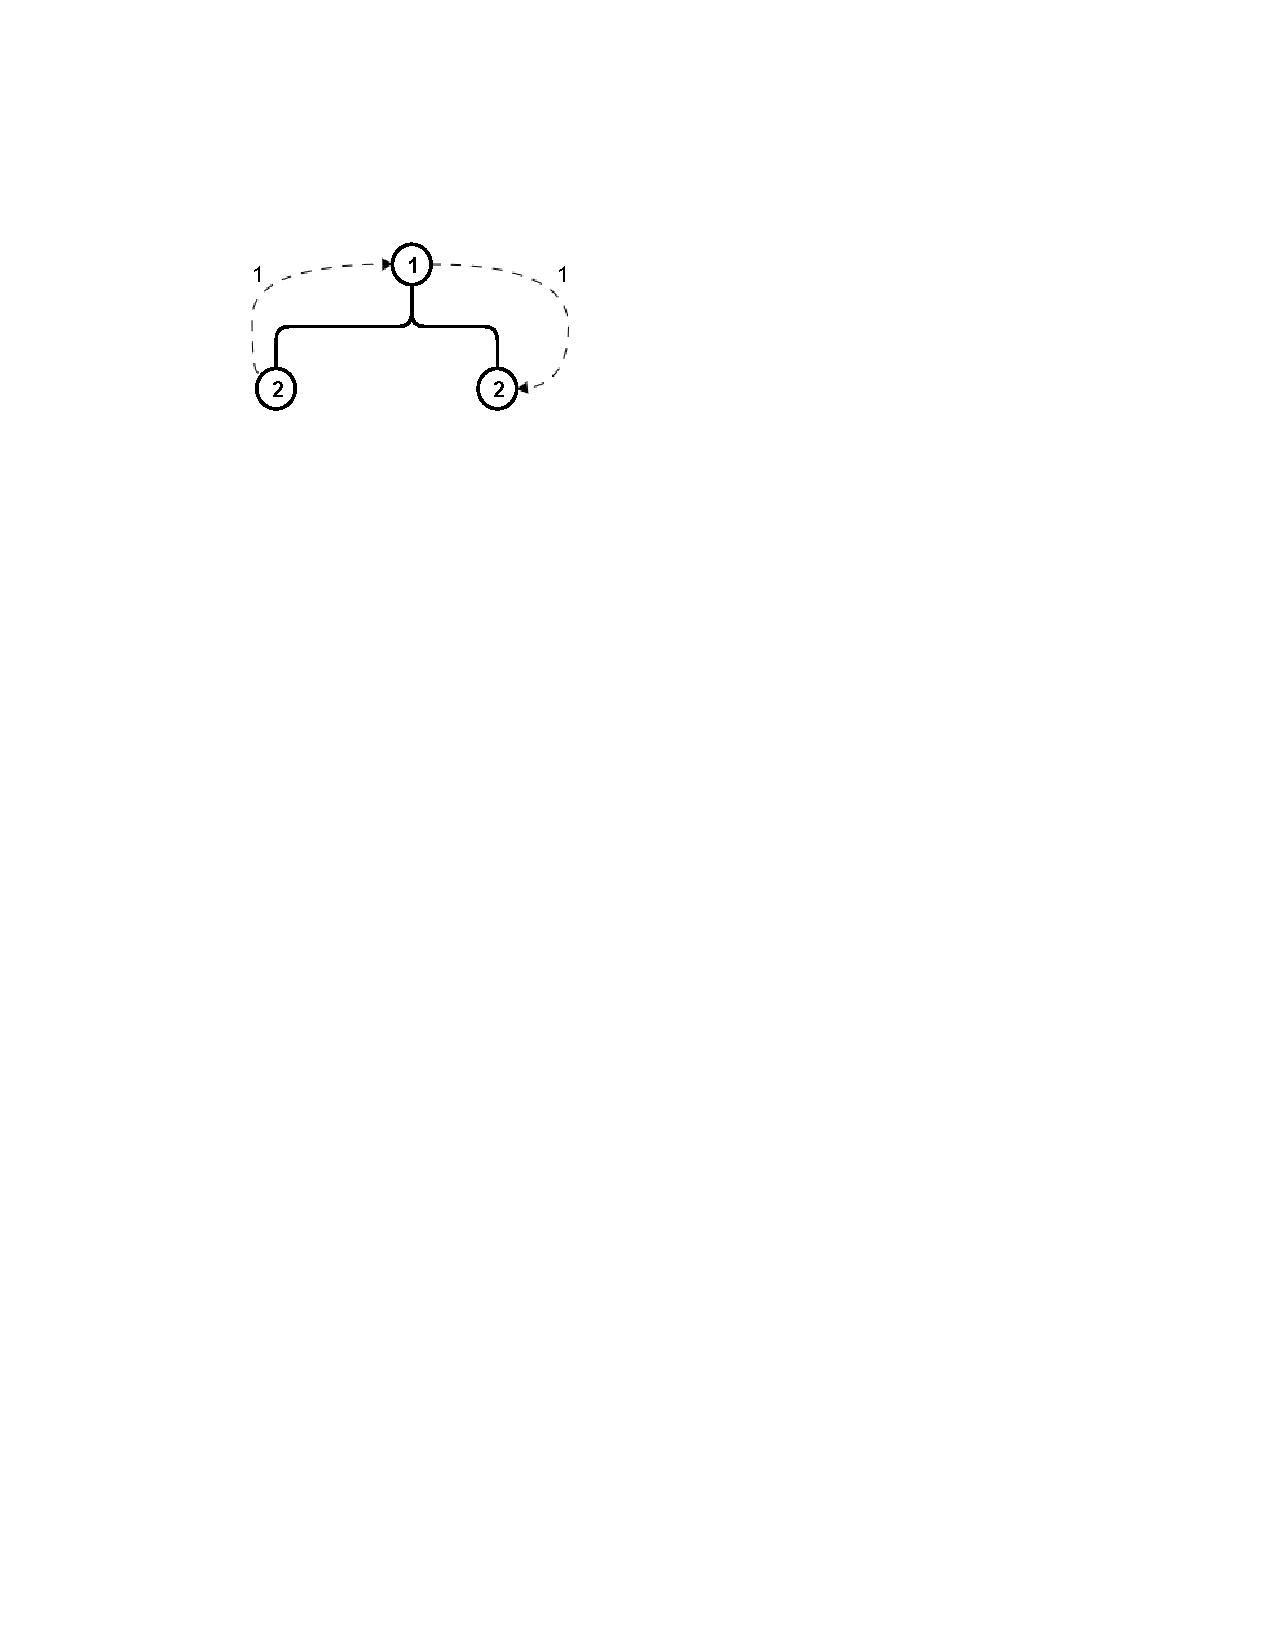
\includegraphics{figures/distance_two_buses.pdf}
        \caption{The distance between two neighbor buses}
        \label{fig:distance_two_buses}
    \end{figure}
\bigskip
\\The hierarchy of branches is similar to the hierarchy of buses. The branch, which connects feeder bus and buses in the first hierarchy, is defined as the branch in the first hierarchy, and the branch which connects buses in the $(n-1)^{th}$ hierarchy and buses in the $n^{th}$ hierarchy belongs to the $(n-1)^{th}$ branches hierarchy as shown in Figure \ref{fig:radial hierarchy}. But the fact that there is one thing different between the buses and branches is the buses which connect to the same bus at an upper hierarchy are not connected together as introduced in the last paragraph. But all the branches connected to one bus are assumed to connect together, which means in this case the distance between two branches connected to the same bus is 1. After defining the hierarchy index of buses and branches, the hierarchy of each bus or branch should be found by using Breadth-First search(BFS) algorithm which is widely used for searching tree or graph structure system.

\subsection{Path of Radial Network}
After giving the definition of the hierarchy of the buses and branches in the radial network, the concept of the path in a radial network should be introduced. In this project, the paths in the radial network are defined as a group of connected buses and branches, which go from the feeder bus to a "leaf" bus.
    \begin{figure}[!h]
        \centering
        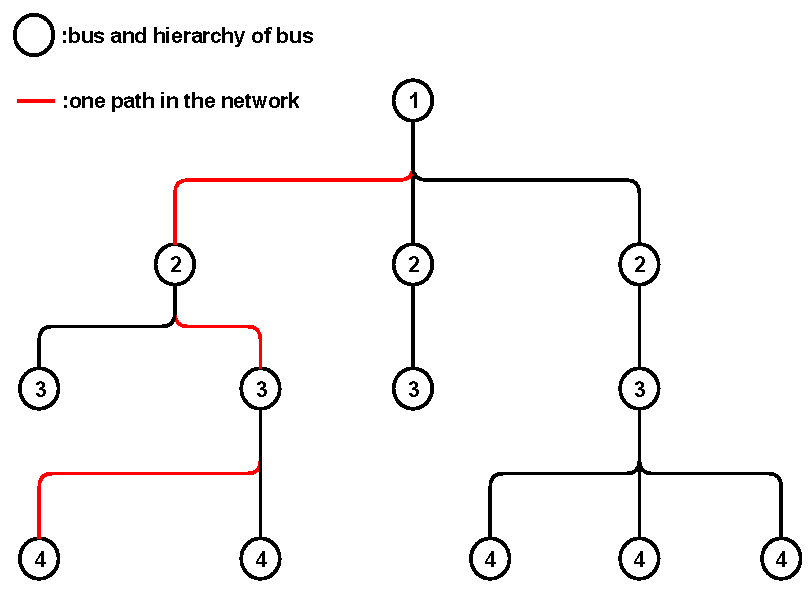
\includegraphics[ height=8cm, width=12cm]{figures/path_radial_network.pdf}
        \caption{One path in radial network}
        \label{fig:path_radial_network}
    \end{figure}
Figure \ref{fig:path_radial_network} is a schematic diagram showing one of the seven paths in the radial network which is marked by a red line. The whole process is similar to the BFS except that the path search is from the bottom to the top and only the buses at higher hierarchy are searched. The pseudo code for finding the paths $Path$ is shown in the Appendix 5.3. 


\subsection{Influence of Smart Meters Distance to the Feeder Bus}
This section investigates the influence of the distance of meters to the feeder bus on the accuracy of estimators. The influence of bus meters and branch meters is investigated separately. Due to the fact that the voltage magnitudes and power flows are key quantities desired by DSO, only the accuracy of the bus voltage magnitudes and active and reactive power flows on the branches are considered as the criterion for the performance of estimators. The RMSE over 96 time steps is used as a metric. Taking the voltage magnitude as an example, one RMSE at each of the 206 buses, for each of the 30 scenarios and for each of the 100 corresponding cases is calculated. The mean $RMSE$ voltage magnitude across 206 buses for case $i$ in scenario $j$ is defined as follows:
\begin{align}
    RMSE^V_{i,j} &= \frac{1}{206} \sum_{k=1}^{206} RMSE_{i,j}(V^k)
    \label{eq:RMSE_V}
\end{align}
, where $RMSE^V_{i,j}$ represents the mean $RMSE$ value of the $i^{th}$ case in scenarios $j$ for all 206 buses in this thesis. $RMSE_{i,j}(V^k)$ indicates the voltage magnitude RMSE for the $k^{th}$ bus of the $i^{th}$ case in scenario $j$. Similarly, the active and reactive power flow error for the $i^{th}$ case in scenarios $j$ can be represented as $RMSE^{P_{flow}}_{i,j}$ and $RMSE^{Q_{flow}}_{i,j}$, respectively.
\bigskip
\\After showing the performance criteria for each case, the distance of the smart meters to the feeder bus can be defined. For instance, the distance from one bus meter at bus $v_i$ to the feeder bus $v_1$ is defined as:
\begin{align}
    dist_{i,j}(v_k) &= m^{v_k}_{i,j} ( hier(v_k) - hier(v_k) )
    \label{eq:dist_one_bus}
\end{align}
, where $dist_{i,j}(v_k)$ represents the distance from the smart meter at bus $v_k$ to the feeder bus $v_1$ of case $i$ in scenario $j$, and $m^{v_k}_{i,j}$ is a binary variable which indicates if there is a bus meter at bus $v_k$ of case $i$ in scenario $j$. $m^{v_k}_{i,j}$ equals to 1 if there is a bus meter at bus $v_k$ and equals to 0 if there is no meter at bus $v_k$. With the help of the hierarchy of each bus defined before, the distance from each bus meter to the feeder bus can be obtained easily. Then, the total distance $dist^{bus}_{i,j}$ from all bus meters to the feeder bus of the case $i$ in scenario $j$ can be calculated by:
\begin{align}
    dist^{bus}_{i,j} &= \sum_{k=1}^{206} dist_{i,j}(v_k)
    \label{eq:dist_bus}
\end{align}
And the branch meters distance to the feeder bus $dist^{branch}_{i,j}$ from all branch meters to the branches connected to the feeder bus of the case $i$ in scenario $j$ can be calculated in the same way. Nevertheless, notice that if there are two branch meters connected at the same branch, they are counted as one branch meter, because there is no significant influence on the accuracy of the estimator between one meter or two meters on the same branch.
\bigskip
\\After obtaining the bus and branch meter distances to the feeder bus for 100 cases in each scenario and the corresponding $RMSE_j^V$, $RMSE_j^{P_{flow}}$ and $RMSE_j^{Q_{flow}}$ which represents the $RMSE$ for 100 case in scenario $j$ for $j=1,2,\cdots,30$, where $RMSE_j^V=\{RMSE_{1,j}^V,RMSE_{2,j}^V,\cdots,RMSE_{100,j}^V \}$, $\{RMSE_{1,j}^{P_{flow}},RMSE_{2,j}^{P_{flow}},\cdots,RMSE_{100,j}^{P_{flow}} \}$, and $\{RMSE_{1,j}^{Q_{flow}},RMSE_{2,j}^{Q_{flow}},\cdots,RMSE_{100,j}^{Q_{flow}} \}$, the Spearman's correlation coefficient is used as explained before in Sect. \ref{sect:spearman}. Take the bus meters as an example, the Spearman's correlation coefficient $p(RMSE_j^V,dist_j^{bus})$ between the voltage magnitude $RMSE_j^V$ and distance of the bus meters to the feeder bus $dist_j^{bus}=\{dist_{1,j}^{bus},dist_{2,j}^{bus},\cdots,dist_{100,j}^{bus} \}$ in scenario $j$ can be calculated by Equation \ref{eq:spearman factor}. After calculating the Spearman's correlation coefficient $p(RMSE_j^V,dist_j^{bus})$ since $j=1,\cdots,30$, the mean Spearman correlation coefficient is defined as $p(RMSE^V,dist^{bus})$.
\bigskip
\\The process for detecting the Spearman's correlation coefficient between the distance of branch meters to the feeder bus and different types of error is the same as the one with bus meters. 
    
\subsubsection{Result of the Influence of Meter Distance to Feeder Bus}
    \begin{table}[!h]
        \centering
        \begin{tabular}{c|c|c|c|c}
             & WLS & EKF & SHGM & SVR-EKF\\ \hline
            $p(RMSE^V,dist^{bus})$ & 0.0821($vw$) & 0.0839($vw$) & 0.0816($vw$) &  0.1295($vw$)\\
            $p(RMSE^{P_{flow}},dist^{bus})$ & 0.0647($vw$) & 0.0667($vw$) & 0.0662($vw$) &  0.0582($vw$)\\
            $p(RMSE^{Q_{flow}},dist^{bus})$ & 0.0915($vw$) & 0.0937($vw$) & 0.0846($vw$) &  0.0797($vw$)\\
            $p(RMSE^V,dist^{branch})$ & 0.1521($vw$) & 0.1404($vw$) & 0.0848($vw$) &  0.1539($vw$)\\
            $p(RMSE^{P_{flow}},dist^{branch})$ & 0.1003($vw$) & 0.0936($vw$) & 0.1120($vw$) &  0.1473($vw$)\\
            $p(RMSE^{Q_{flow}},dist^{branch})$ & 0.1074($vw$) & 0.0963($vw$) & 0.1025($vw$) &  0.1288($vw$)\\
        \end{tabular}
        \caption{Mean Spearman coefficient of meter distance to feeder bus and RMSE}
        \label{tab:spearman_meter_dist}
    \end{table}
\noindent    
Table \ref{tab:spearman_meter_dist} shows the mean value of the Spearman's correlation coefficient across 30 scenarios between bus or branch meters distance to the feeder bus and the error in the estimation of voltages, active and reactive power flows. The details of the Spearman coefficient value can be found in Appendix A.1. It can be seen from the table that the correlation is very weak in all cases. Hence, it can be concluded that the distances of bus or branch meters to the feeder bus have no influence on the accuracy of estimated voltage magnitude, active power flow, and reactive power flow for these four estimators.

\subsection{Influence of Smart Meters Distribution}
This section investigates the influence of the distribution of bus meters and branch meters on the accuracy of estimators. 
\subsubsection{Definition of Meter Distribution}
The aim of this section is to define how to identify if bus meters or branch meters are well distributed or not. For instance, the $dist_{i,j}^{close}{ ( v_k ) }$ corresponds to the distance from bus $v_k$ to the closest bus with a meter for case $i$ in scenario $j$. Once all $dist_{i,j}^{close}{ ( v_k ) }$ for all of the buses are calculated, they are summed together and the total distribution factor $distr^{bus}_{i,j}$ for the bus meters at the $i^{th}$ case in scenario $j$ can be obtained:
\begin{align}
    distr^{bus}_{i,j} &= \sum_{k=1}^{206} dist_{i,j}^{close}{(v_k)}
    \label{eq:distr_bus}
\end{align}
And the distribution factor $distr^{branch}_{i,j}$ of branch meters in case $i$ of scenario $j$ can be obtained with the same method by summing the distance from each branch $e_i$ to the closest branch with a meter:
\begin{align}
    distr^{branch}_{i,j} &= \sum_{k=1}^{205} dist_{i,j}^{close}{(e_k)}
    \label{eq:distr_branch}
\end{align}
If the value of $distr^{bus}_{i,j}$ is small, it means that there is a bus meter close to each bus and the bus meters are well distributed acorss the system. On the contrary, the bus meters are not well distributed when $distr^{bus}_i$ is larger, meaning that meters are mainly concentrated at a few buses.

\subsubsection{Searching the Closest Meter by BFS}
\label{sect:BFS_dist}
Before calculating the distribution factor $distr$, it is necessary to get the distance $dist_{i,j}^{close}{ ( v_k ) }$ from each bus $v_k$ to its closest meter for $k=1,\cdots,206$ in the $i^{th}$ case of the $j^{th}$ scenario. There are two definitions for the closest metered bus to each bus, through Breath-First Search (BFS) or Path Search.
    \begin{figure}[!h]
        \centering
        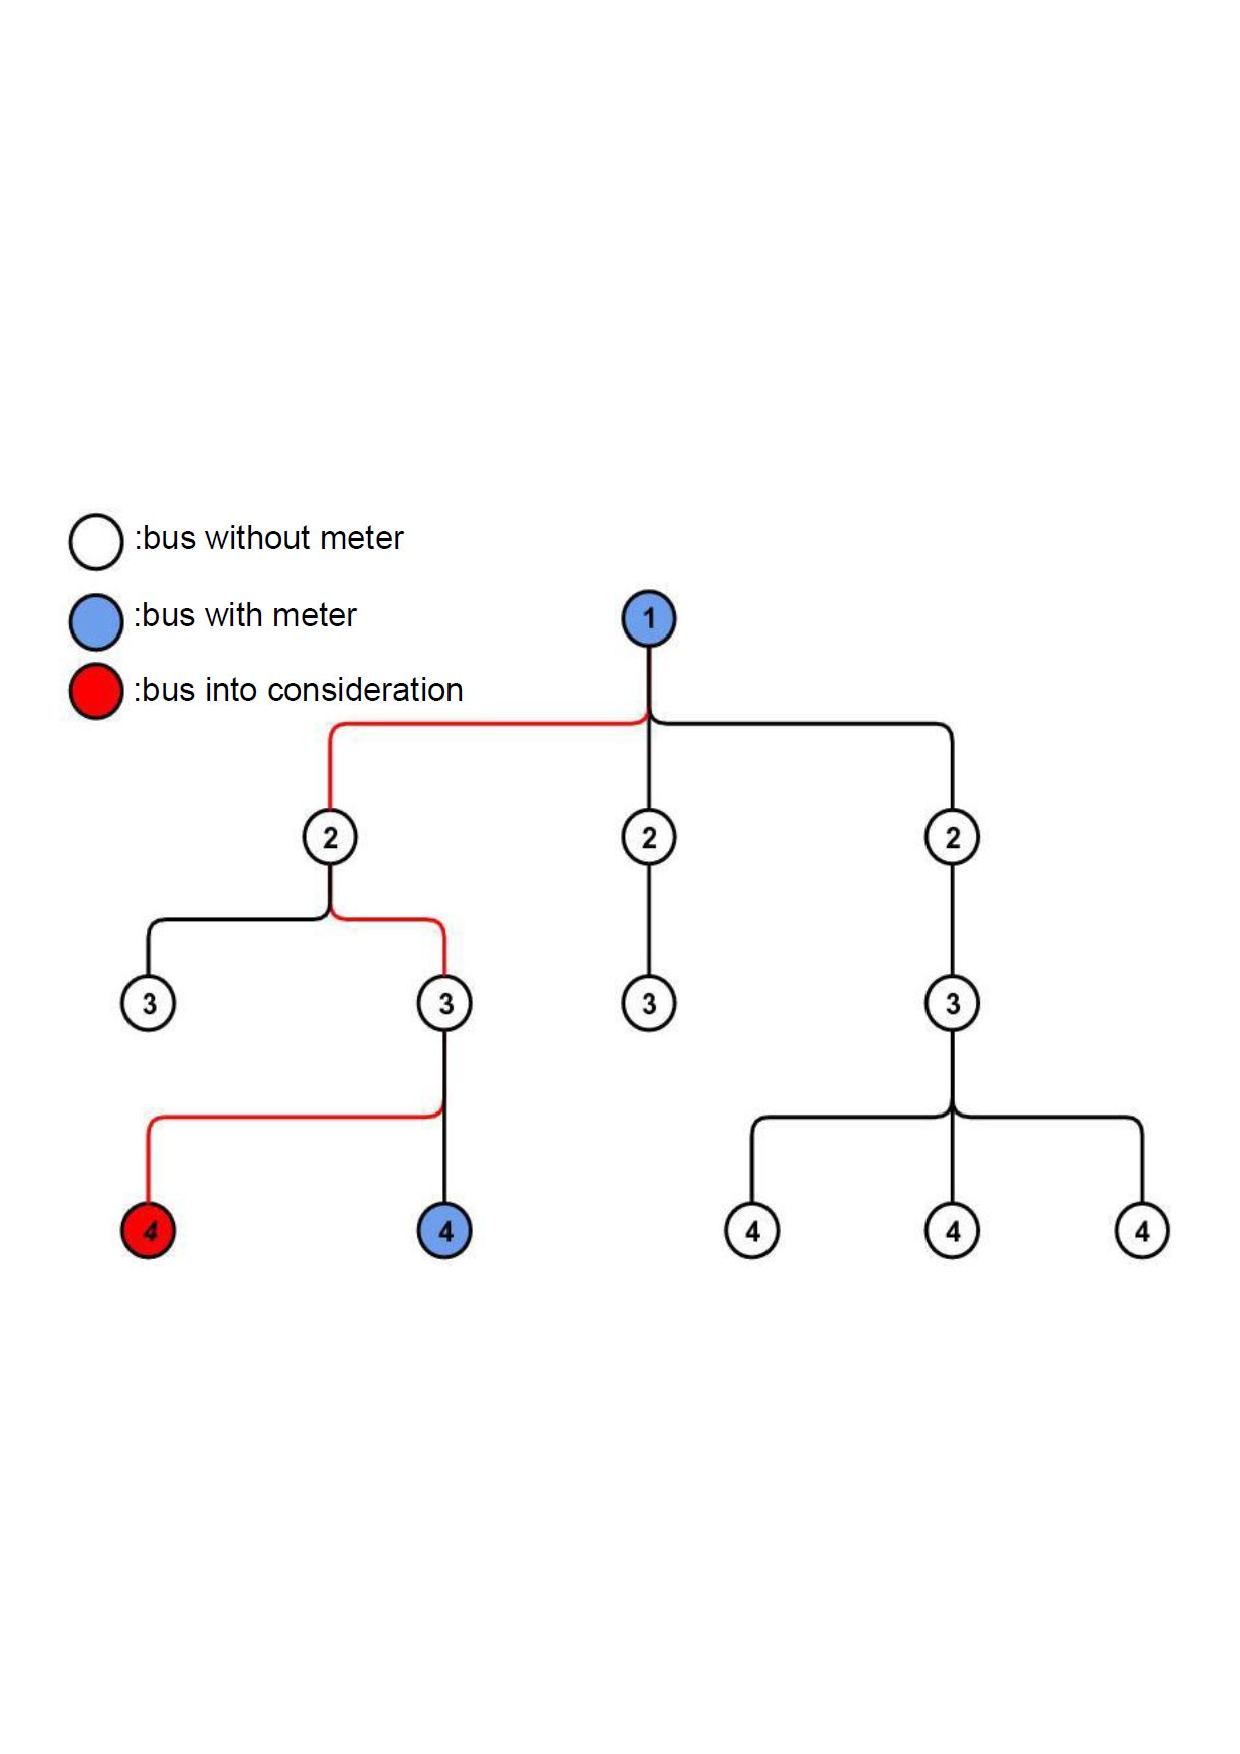
\includegraphics[ height=9cm, width=14cm]{figures/topo_new.pdf}
        \caption{Two method for obtaining $dist_{i,j}^{close}{ ( v_{red} ) }$}
        \label{fig:distr_topo}
    \end{figure} 
\bigskip
\\Figure \ref{fig:distr_topo} shows a simplified distribution grid with 13 buses where the blue buses have a meter and the red line shows the path connected with the red bus which is considered. By using BFS, the closest bus meter to the red bus is the blue one at the fourth hierarchy. So, $dist_{i,j}^{close}{(v_{red})}=2$ in this case based on BFS. Analogously, the distance $dist_{i,j}^{close}{(e_i)}$ from  to the branch $e_i$ to its closest branch meter can be obtained with the same method. The pseudo-code for the whole procedure can be found in Appendix 5.3.3.
\bigskip
\\After finding the distance from each bus or branch to their closest metered bus or branch, the distribution of bus meters $distr_{i,j}^{bus}$ and branch meters $distr_{i,j}^{branch}$ for case $i$ in scenario $j$ can be calculated by Equation \ref{eq:distr_bus}. And the Spearman's correlation coefficients between meter distribution and the different errors in consideration, for the four estimators and for each scenario can be obtained, whose details are shown in Appendix A.1. FOr instance, $p(RMSE_j^V,distr_j^{bus})$ represents the Spearman correlation coefficient between mean voltage magnitude error $RMSE_j^V=\{RMSE_{1,j}^V,RMSE_{2,j}^V,\cdots,RMSE_{100,j}^V \}$ and bus meters distribution $distr_j^{bus}=\{distr_{1,j}^{bus},distr_{2,j}^{bus},\cdots,distr_{100,j}^{bus} \}$ based on BFS in scenario $j$. After that, the mean Spearman's factor $p(RMSE_j^V,distr_j^{bus})$ for 30 scenarios and for  each estimator can be calculated. Similarly, the Spearman correlation coefficient for the other types of error and meters distribution based on BFS can be calculated, and their values are listed in Table \ref{tab:spearman_meter_distr_BFS}. It can be seen that all the mean Spearman's correlation coefficients show a very weak correlation, well below the threshold 0.3. As a result, the conclusion can be drawn that the distribution of bus meters and branch meters based on BFS does not influence the voltage magnitude error $RMSE^V$, active power flow error $RMSE^{P_{flow}}$, and reactive power flow error $RMSE^{Q_{flow}}$ for the four state estimation algorithms.

    \begin{table}[!h]
        \centering
        \begin{tabular}{c|c|c|c|c}
             & WLS & EKF & SHGM & SVR-EKF\\ \hline
            $p(RMSE^V,distr^{bus})$ & 0.0664($vw$) & 0.0609($vw$) & 0.0584($vw$) &  0.0847($vw$)\\
            $p(RMSE^{P_{flow}},distr^{bus})$ & 0.0916($vw$) & 0.0900($vw$) & 0.0942($vw$) &  0.1073($vw$)\\
            $p(RMSE^{Q_{flow}},distr^{bus})$ & 0.0917($vw$) & 0.0970($vw$) & 0.0919($vw$) &  0.0843($vw$)\\
            $p(RMSE^V,distr^{branch})$ & 0.0964($vw$) & 0.0955($vw$) & 0.0766($vw$) &  0.1143($vw$)\\
            $p(RMSE^{P_{flow}},distr^{branch})$ & 0.2759($w$) & 0.2063($w$) & 0.2150($w$) &  0.1556($vw$)\\
            $p(RMSE^{Q_{flow}},distr^{branch})$ & 0.2755($w$) & 0.2325($w$) & 0.2493($w$) &  0.1694($vw$)\\
        \end{tabular}
        \caption{Mean Spearman Coefficient of Meter Distribution by BFS and RMSE}
        \label{tab:spearman_meter_distr_BFS}
    \end{table}


\subsubsection{Searching the Closest Meter by Path Search}
\label{sect:Path_dist}
Another definition of $dist_{i,j}^{close}{(v_i)}$ is searching the closest distance from bus $v_i$ to a metered bus only on the same path. For example in Figure \ref{fig:distr_topo}, the closest metered bus to the red bus is the blue one on the fourth hierarchy on the left whose $dist_{i,j}^{close}{(v_{red})}$ equals to 2 according to BFS. However, these two buses do not lie on the same path. The closest metered bus on the same path is the feeder bus at the first hierarchy whose distance $dist_{i,j}^{close}{(v_{red})}$ is 3. As a result, a different value of $dist_{i,j}^{close}{(v_i)}$ is obtained based on Path Searching and results in a different value of the total meter distribution value $distr_{i,j}^{bus}$ or $distr_{i,j}^{branch}$ for metered buses and branches in the $i^{th}$ case of scenario $j$, respectively. And the pseudo-code for searching the distance $dist_{i,j}^{close}{(v_{red})}$ from bus $v_{red}$ to its closest metered bus by Path Search for case $i$ in scenario $j$ is shown in Algorithm \ref{alg:searching meter PS}, where $M_{i,j}^{bus}= \{v_1,\cdots,v_m \}$ is the set of buses who have a metered bus in the $i^{th}$ case of scenario $j$, $p_i=(p_i^v,p_i^e)$ is the $i^{th}$ path, and $Path=(p1,\cdots,p_{np})$ includes all paths in system $G=(V,E)$.

\bigskip
\begin{algorithm}[H]
\KwData{G=(V,E), M_{i,j}^{bus}, Path=(p1,\cdots,p_{np}), p_i=(p_i^v,p_i^e)}
\KwResult{dist_{i,j}^{close}{(v_{red})}}
\Initialize{\textbf{Initialize:} $L=\{v_{red}\}$, $k=0$, $a=\infty$\;}

\eIf{$L$ \cap $M_{i,j}^{bus}$ \neq $\emptyset$}
{$dist_{i,j}^{close}{(v_{red})} = k$}
{$do \, nothing$}
\For{p_i \in Path}{
    \eIf{$v_{red}$ \in $p_i^v$}
    {
        $M^s = p_i^v \cap M_{i,j}^{bus}$\;
        \For{$m \in M^s$}{
            $b=|hier(m)-hier(v_{red})|$
            \eIf{$b<a$}{
                $dist_{i,j}^{close}{(v_{red})} = b$\;
            }{
                $do$ \, $nothing$
            }            
        }
        
    }
    {
        $do \, nothing$
    }
}
\caption{Searching $dist_{i,j}^{close}{(v_{red})}$ by Path Search}
\label{alg:searching meter PS}
\end{algorithm}

\bigskip
\noindent
\\Notice that there is always at least one bus meter installed at the feeder bus at the same path with $v_{red}$. However, there might be no metered branch connected on the same path as the branch $e_{red}$. As a result, when there is no metered branch along the path of branch $e_{red}$, the distance $hier(e_s)-hier(e_1)$ between feeder branch and its closest meter at branch $e_s$ must be added to $hier(e_{red})-hier(e_1)$ to get the distance from branch $e_{red}$ to its closest metered branch:
\begin{align}
    dist_{i,j}^{close} (e_{red}) &= hier(e_s)-hier(e_1) + hier(e_{red}) - hier(e_1)
    \label{eq:branch_meter_path}
\end{align}
After obtaining the $dist_{i,j}^{close}$ for all of the buses and branches for cases $i$ in scenario $j$, the distribution factor $distr$ for metered buses and branches can be calculated by Equation \ref{eq:distr_bus} and \ref{eq:distr_branch}. Then, the Spearman's correlation coefficient between bus or branch meters distribution and error can be calculated for each scenario, which is shown in Appendix A.1. By calculating the mean value of Spearman's factor over 30 scenarios, Table \ref{tab:spearman_meter_distr_path} can be obtained.
    \begin{table}[!h]
        \centering
        \begin{tabular}{c|c|c|c|c}
             & WLS & EKF & SHGM & SVR-EKF\\ \hline
            $p(RMSE^V,distr^{bus})$ & 0.0776($vw$) & 0.0904($vw$) & 0.0975($vw$) &  0.0858($vw$)\\
            $p(RMSE^{P_{flow}},distr^{bus})$ & 0.0982($vw$) & 0.1030($vw$) & 0.1031($vw$) &  0.0970($vw$)\\
            $p(RMSE^{Q_{flow}},distr^{bus})$ & 0.0991($vw$) & 0.1024($vw$) & 0.0938($vw$) &  0.0831($vw$)\\
            $p(RMSE^V,distr^{branch})$ & 0.2346($w$) & 0.2516($w$) & 0.0977($vw$) &  0.3823($w$)\\
            $p(RMSE^{P_{flow}},distr^{branch})$ & 0.3295($w$) & 0.2934($w$) & 0.3183($w$) &  0.4037($m$)\\
            $p(RMSE^{Q_{flow}},distr^{branch})$ & 0.3453($w$) & 0.2691($w$) & 0.3358($w$) &  0.3355($w$)\\
        \end{tabular}
        \caption{Mean Spearman Coefficient of Meter Distribution by path and RMSE}
        \label{tab:spearman_meter_distr_path}
    \end{table}
\bigskip
\\The first three rows in Table \ref{tab:spearman_meter_distr_path} show the mean Spearman's coefficient between the bus meter distribution and three types of errors. All of them show a very weak correlation between bus meters distribution and the $RMSE$ , well below 0.3. In addition, the distribution of the branch meters has no significant influence on the accuracy of the voltage error $RMSE^V$ where nearly all of the Spearman's factors are below but close to 0.3 except SVR-EKF. However, almost all of the Spearman's correlation coefficients between branch meters distribution and power flow errors are higher than 0.3 (except EKF). Hence, it can be concluded that the distribution of the branch meters based on Path Search influences the active power flow error $RMSE^{P_{flow}}$ and reactive power flow error $RMSE^{Q_{flow}}$. The better distributed the branch meters are, the lower the power flow error.

\subsubsection{Summary}
Based on the previous simulation results of meters distribution on the estimators' accuracy, it can be seen that the meter distribution method based on BFS has no influence on the mean $RMSE^V$, $RMSE^{P_{flow}}$, and $RMSE^{Q_{flow}}$. Also, the bus meters distribution based on Path Search has no influence on the mean $RMSE^V$, $RMSE^{P_{flow}}$, and $RMSE^{Q_{flow}}$ for the tested four estimators in the radial distribution grid. But $RMSE^{P_{flow}}$ and $RMSE^{Q_{flow}}$ can be reduced by properly distributing the branch meters based on the Path Search. Since the above errors can be reduced when $distr^{branch}$ is smaller, for a giving number of branch meters, it is better to install them as well distributed as possible based on the Path Search.

\subsection{Influence of Bus Meters Location based on Power Injection}
This section investigates the location bus meters for increasing the accuracy of the state estimation algorithms. The original idea is that the accuracy of the pseudo-measurements at different buses is different. If the given bus meters are installed at the buses whose potential pseudo-measurements are not accurate, then the pseudo-measurements with high mismatch can be avoided, and the performance of the estimators can be increased by increasing the accuracy of pseudo-measurements. As a result, the aim is to find the buses whose potential pseudo-measurements have low accuracy and install smart bus meters at these buses.

\subsubsection{Influence of Pseudo-Measurements Accuracy on State Estimation}
The first step is to detect if the accuracy of the pseudo-measurements has an influence on the performance of the state estimation algorithms. Assuming $p_{psu-inj}^i(t)$ is the $i^{th}$ pseudo active power injection measurement at time step $t$ and $p_{inj}^i(t)$ is its corresponding real value. Then, the total active power mismatch $mis^{P}$ for all pseudo active power injection and 96 time steps at this case is:
\begin{align}
    mis^{P} &= \sum_{i=1}^{m_p} \sum_{t=1}^{96} |p_{psu-inj}^i(t)-p_{inj}^i(t)|
    \label{eq:total_mismatch}
\end{align}
, where $m_p$ is the total number of pseudo active power injection measurements in the grid. The total reactive power mismatch $mis^{Q}$ for each case can be calculated in the same way. The Pearson correlation coefficient between active power mismatch and its corresponding mean voltage, active and reactive power flow error over 100 cases for each scenario can be derived, respectively. In this project, only the influence of the active power injection mismatch $mis^{P}$ is investigated because the power factor of the loads is assumed to be constant, which means that the changing tendency between active power injection and reactive power injection is nearly the same.
    \begin{table}[!h]
        \centering
        \begin{tabular}{c|c|c|c|c}
             & WLS & EKF & SHGM & SVR-EKF\\ \hline
            $r(RMSE^V,mis^{P})$ & 0.1959($vw$) & 0.1851($vw$) & 0.2212($w$) &  0.2528($w$)\\
            $r(RMSE^{P_{flow}},mis^{P})$ & 0.4883($m$) & 0.4975($m$) & 0.5878($m$) &  0.6418($s$)\\
            $r(RMSE^{Q_{flow}},mis^{P})$ & 0.3460($m$) & 0.3535($m$) & 0.3837($m$) &  0.4241($m$)\\
        \end{tabular}
        \caption{Mean Pearson Coefficient between active power injection mismatch and RMSE}
        \label{tab:pearson_mis_error}
    \end{table}
Table \ref{tab:pearson_mis_error} shows the mean Pearson's coefficients between the total active power injection mismatch and the error in state estimation over 30 scenarios. It can be seen that there is a overall moderate to strong relation between the total active power injection mismatch and both active and reactive power flow errors. The mean correlation with the voltage error is very week (i.e., lower than the defined threshold of 0.3). However, when looking at the result for each individual scenario, it appears that the voltage error is strongly correlated with the total mus injection mismatch whenever there a no power flow measurements but smart meters also provide information about the voltage (i.e., scenarios 10 and 19).
    \begin{figure}[!h]
        \centering
        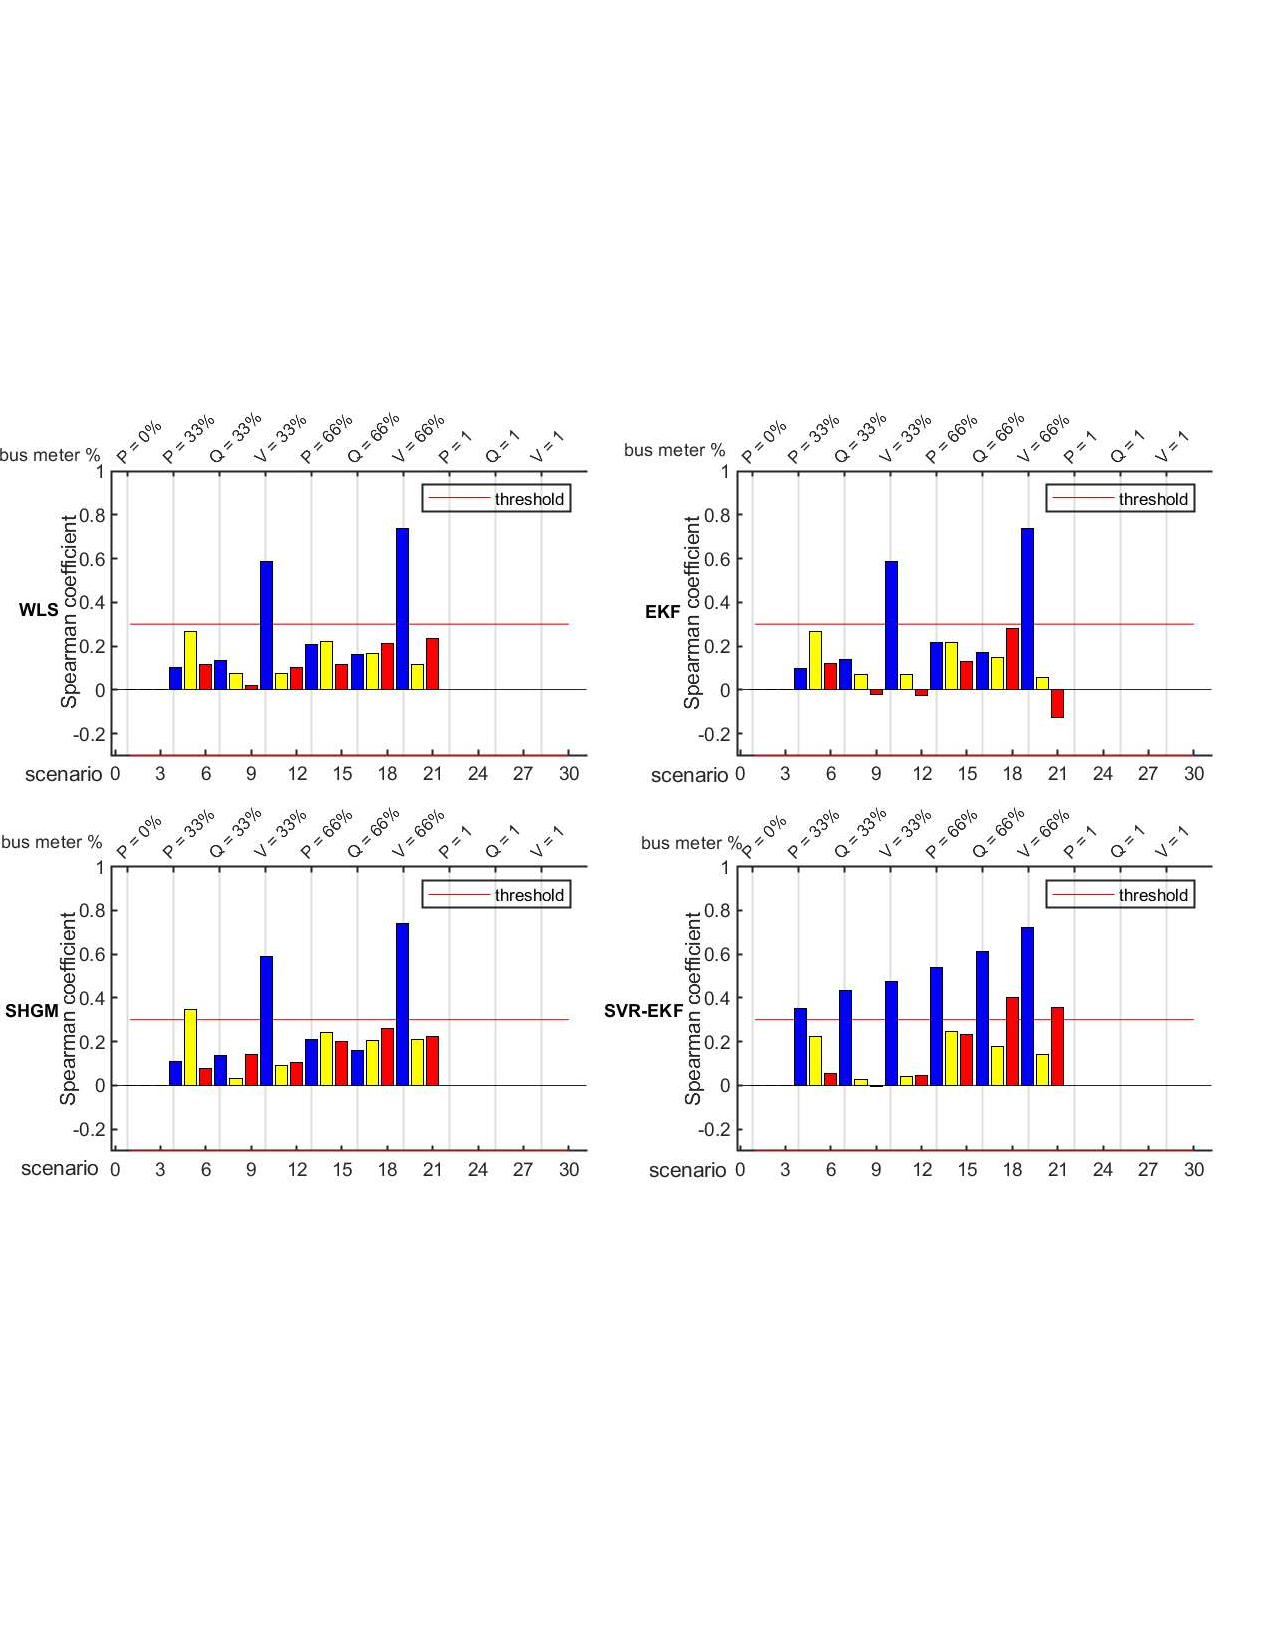
\includegraphics[ height=9cm, width=14cm]{figures/mis_pinj_error.pdf}
        \caption{Pearson's coefficient $r(RMSE^V,mis^{P})$ for 30 scenarios}
        \label{fig:mis_Pinj_error}
    \end{figure} 
For SVR-EKF, $r(RMSE^V,mis^{P})$ is higher than the threshold of 0.3 as long as there is no power flow measurements. The correlation coefficients from scenario 1 to 3 are zero because all of the active power injections are pseudo measurements and $mis^{P}$ is therefore constant. Concerning scenarios 22 to 30 the active power injection for all the buses are measured such that there is no pseudo-measurements for active power injection.
\bigskip
\\To conclude, the accuracy of the pseudo-measurements for active power have an influence on the result of power flow. As for the voltage magnitude accuracy for WLS, EKF, and SHGM, it can only be influenced by the placement of smart meters whenever they provide voltage information. Finally, the voltage magnitude error in SVR-EKF is correlatied with the accuracy of the pseudo
active power injection only if there are no branch meters.

\subsubsection{Accuracy of Pseudo-Measurements}
After knowing that the accuracy of the pseudo active power injection has an effect on the accuracy of the estimators, it is important to investigate the methods for improving the accuracy of the pseudo-measurements. The idea is that nearly all the loads in this project are residential consumers, which means that their active power injection can be very volatile within one day. So, the hypothesis is made that the total mismatch between the pseudo active power injection and its corresponding real value at bus $i$ $P^{mis}_i$ for one day is high when the total active energy consumption $E_c^i$ at bus $i$ for one day is high. To prove this hypothesis, the Pearson's correlation coefficient $p(P^{mis},E_c)$ between the total active power injection mismatch $P^{mis}= \{ P^{mis}_1,P^{mis}_2,\cdots,P^{mis}_{206} \}$ and the total active energy consumption $E_c= \{E_c^1,E_c^2,\cdots,E_c^{206} \}$ for all buses within one day is calculated. After calculating $p(P^{mis},E_c)$ for 100 cases in 30 scenarios. The boxplot figure with 100 $p(P^{mis},E_c)$ in each of 30 scenarios is shown in Figure \ref{fig:p_tot_p_mis}. Notice that in scenarios 1 to 3, the active power injections at all 205 buses except the feeder bus are pseudo measurements such that there is no difference between the 100 cases from scenario 1 to 3. 
    \begin{figure}[!h]
        \centering
        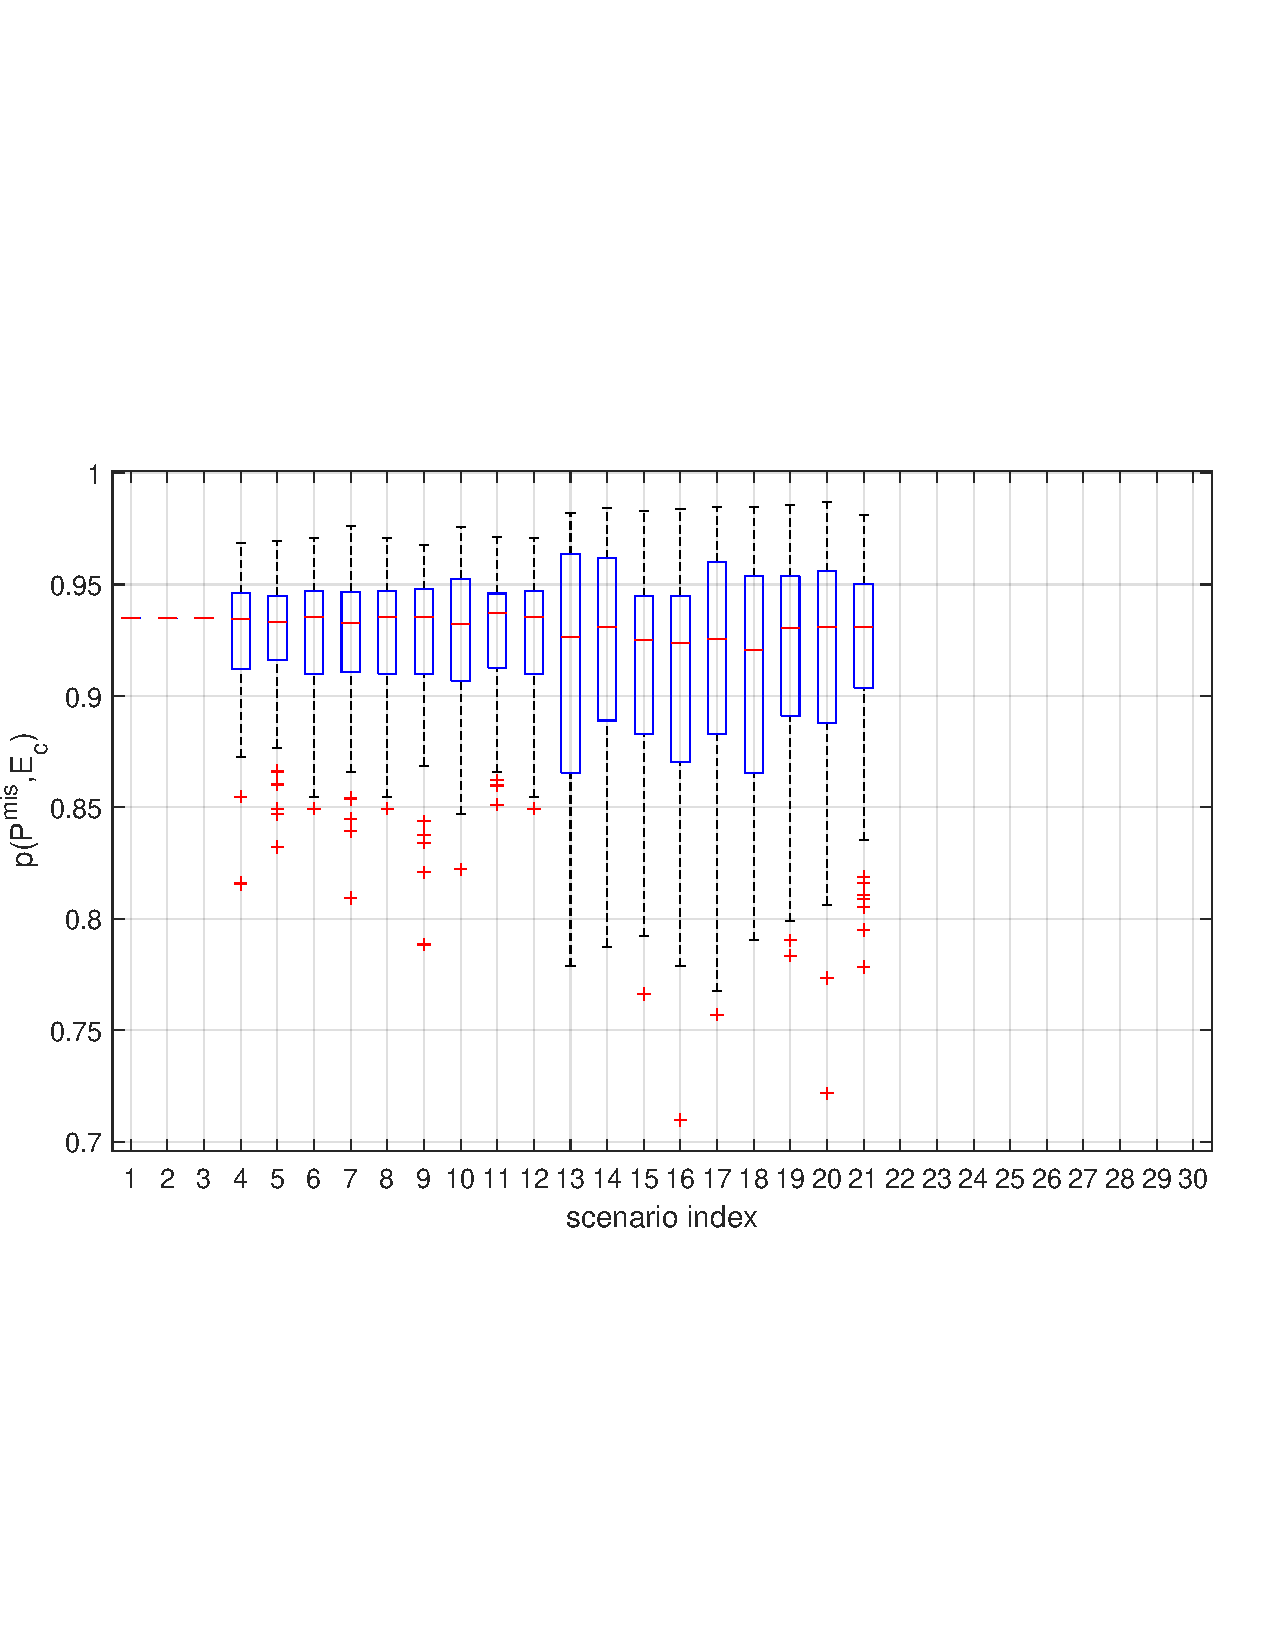
\includegraphics[ height=8cm, width=14cm]{figures/p_tot_p_mis.pdf}
        \caption{100 Pearson's coefficient $p(P^{mis},E_c)$ for 30 scenarios}
        \label{fig:p_tot_p_mis}
    \end{figure}     
In scenarios 22 to 30, there is no pseudo active power injection we cannot compute the correlation. It can be seen that even the lowest $p(P^{mis},E_c)$ is still above 0.7, so the conclusion can be drawn that the accuracy of the pseudo active power injection is reduced when the total power injection at that bus is high.

\subsubsection{Suggested Location for Bus Meters}
By knowing that there is a strong relation between the total active energy consumption and accuracy of its corresponding pseudo active power injection, installing smart meters at the buses whose total active energy consumption is high, the overall accuracy of the pseudo active power injections can be increased. Indeed, the pseudo active power injections would need to be computed at the buses whose total active energy consumption is low, which leads to a higher accuracy on pseudo-measurements. As a result, the accuracy of the estimators can be increased as shown in Table \ref{tab:pearson_mis_error}. For this purpose, the Pearson's correlation coefficient between the active energy consumption  $E^{psu}$ at the buses with pseudo active power injection and the three types of errors $RMSE^{V}$, $RMSE^{P_{flow}}$ ,and $RMSE^{Q_{flow}}$ is calculated for each scenario. The active energy consumption at the buses with pseudo active power injection $E^{tot}$ is calculated by the Equation \ref{eq:E^{psu}}:
\begin{align}
    E^{psu} &= \sum_{i=1}^{m_p} E_c^{v_p^{i}}
    \label{eq:E^{psu}}
\end{align}
, where $E_c^{v_p^{i}}$ is the active energy consumption at bus $v_p^{i}$ which is the $i^{th}$ bus with pseudo active power injection, and $m_p$ is the total number of buses which needs a pseudo active power injection. Because the number of the bus meters is constant for all 100 cases in each scenario, a higher $E^{psu}$ corresponds to a higher mismatch between the pseudo active power injections and their real value , according to the $r(P^{mis},E_c)$ shown in Figure \ref{fig:p_tot_p_mis}.  The Pearson's correlation coefficient between  $E^{psu}$ and the three average errors $RMSE^{V}$, $RMSE^{P_{flow}}$ ,and $RMSE^{Q_{flow}}$ for all 30 scenarios can be found in Appendix A.2. The mean Pearson's correlation coefficient between $E^{psu}$ and these errors over 30 scenarios are shown in Table \ref{tab:pearson_p_tot_error}. 
    \begin{table}[!h]
        \centering
        \begin{tabular}{c|c|c|c|c}
             & WLS & EKF & SHGM & SVR-EKF\\ \hline
            $r(RMSE^V,E^{psu})$ & 0.1851($vw$) & 0.1677($vw$) & 0.1989($vw$) &  0.2825($w$)\\
            $r(RMSE^{P_{flow}},E^{psu})$ & 0.4556($m$) & 0.4651($m$) & 0.5575($m$) &  0.5974($m$)\\
            $r(RMSE^{Q_{flow}},E^{psu})$ & 0.4568($m$) & 0.4643($m$) & 0.5155($m$) &  0.5455($m$)\\
        \end{tabular}
        \caption{Mean Pearson Coefficient of Meter location between $E^{psu}$ and mean RMSE}
        \label{tab:pearson_p_tot_error}
    \end{table}
It can be found that the Pearson's coefficient $r(RMSE^{P_{flow}},E^{psu})$ and $r(RMSE^{Q_{flow}},E^{psu})$ for all of the four estimators are higher than the threshold of 0.3, which proves that the active and reactive power flow errors can be reduced when the bus meters are installed at the buses with high active energy consumption. Similarly, to $r(RMSE^V,mis^P)$, even though the mean value $r(RMSE^V,E^{psu})$ over 30 scenarios is smaller than 0.3 for all four estimators, there are some specific
scenarios where $r(RMSE^V,E^{psu})$ shows a stronger relation as shown in Figure \ref{fig:p_tot_error}.
    \begin{figure}[!h]
        \centering
        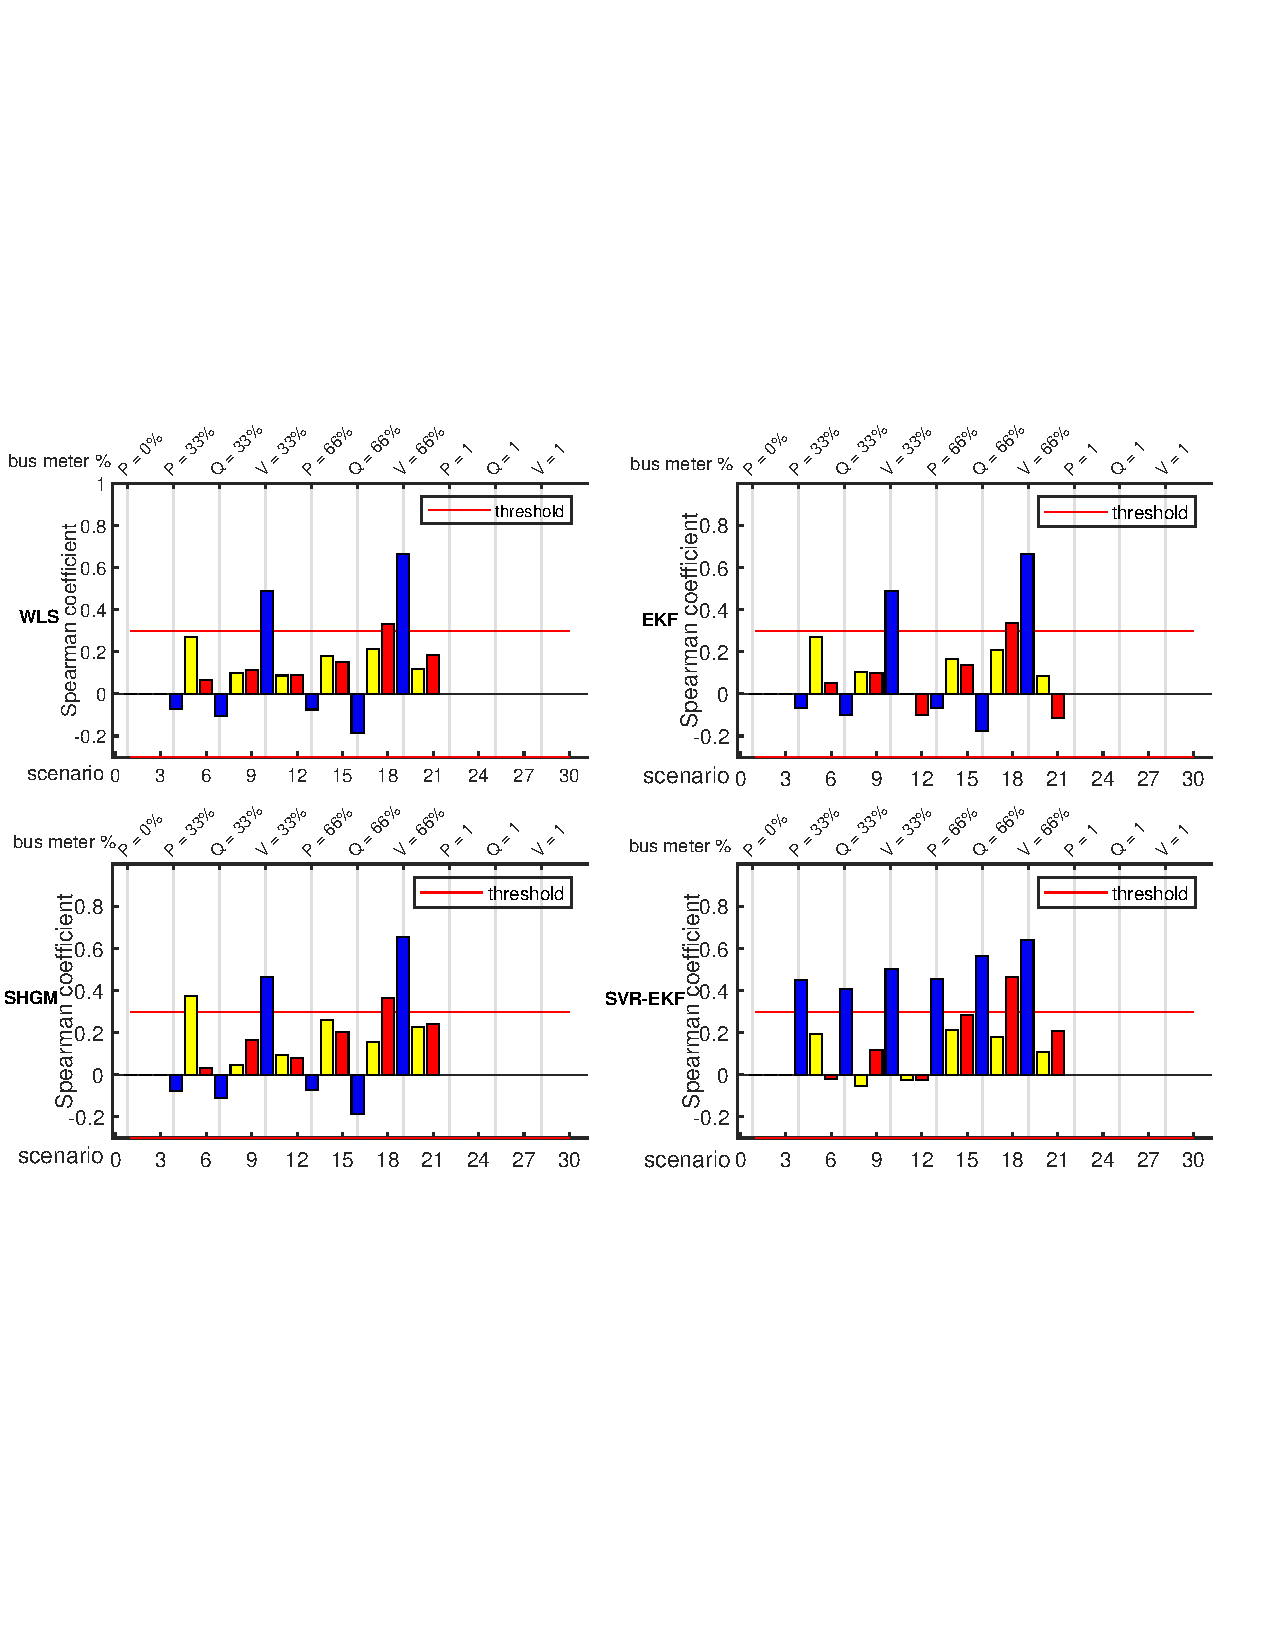
\includegraphics[ height=8cm, width=14cm]{figures/p_tot_error.pdf}
        \caption{Pearson's correlation coefficient between active energy consumption and total active power mismatch for 30 scenarios}
        \label{fig:p_tot_error}
    \end{figure}      
For WLS, EKF, and SHGM, the scenarios 10 and 19 show a moderate to strong relation between the active energy consumption for buses with pseudo measurements and the voltage error $RMSE^V$. Both of them have information for the voltage magnitude but no branch meters are installed. As for SVR-EKF, the Pearman's factor $r(RMSE^V,E^{psu})$ is higher than the threshold 0.3 as long as there is no information for power flows.
\bigskip
\\Based on the analysis above, the conclusion can be drawn that the mean active and reactive power flow error can be reduced by installing the bus meters at the buses whose active energy consumption is known to be generally high. In addition, this can reduce the mean voltage magnitude error when the information of voltage magnitude is also known at the smart meters. To conclude, if there are totally $m^{bus}$ number of bus meters available, the performance of the state estimator can theoretically be improved by installing them at the $m^{bus}$ buses with the highest overall active energy consumption .

\subsection{Testing the Smart Meter Installing Strategy}
Based on the investigation of the influence of the smart meter location on the performance of state estimation algorithms, the following two points can be concluded:
\begin{itemize}
    \item Bus Meter: Installing bus meters at the buses with the highest overall active energy consumption.

    \item Branch Meter: Installing branch meters as well distributed as possible based on the Path Search.
 
    
\end{itemize}
The bus meters installation method is straightforward since the total active energy consumption at all bus can be, in principle, known. As for the location of branch meters, because it is not straighforward to find the optimal case with the lowest value of $distr^{branch}$, the suggested optimal branch meters locations is picked out of the mentioned 100 cases in each of the 30 scenarios. When $10 \% $ of power flow information is known, the smallest $distr^{branch}$ is searched among the scenarios 2, 5, 8, 11, 14, 17, 20, 23, 26, and 29. The smallest $distr^{branch}$ with $20 \%$ of measured power flow is searched within scenarios 3, 6, 9, 12, 15, 18, 21, 24, 27, and 30.
\bigskip
\\After determining the suggested optimal smart meters installation for all 30 scenarios, four state estimation algorithms are run again for each scenario and their accuracy for $RMSE^V$, $RMSE^{P_{flow}}$, and $RMSE^{Q_{flow}}$ is compared with the previously mentioned 100 cases in each scenario.

\subsubsection{Voltage Magnitude Error}
Figure \ref{fig:compare_V} shows the comparison of the voltage error $RMSE^V$ comparison between the proposed optimal smart meter location method and 100 cases in each of 30 scenarios for four estimators. The y-axis is the percentage out of the 100 cases in each scenario which have a higher $RMSE^V$ than the the proposed optimal smart meters location.
    \begin{figure}[!h]
        \centering
        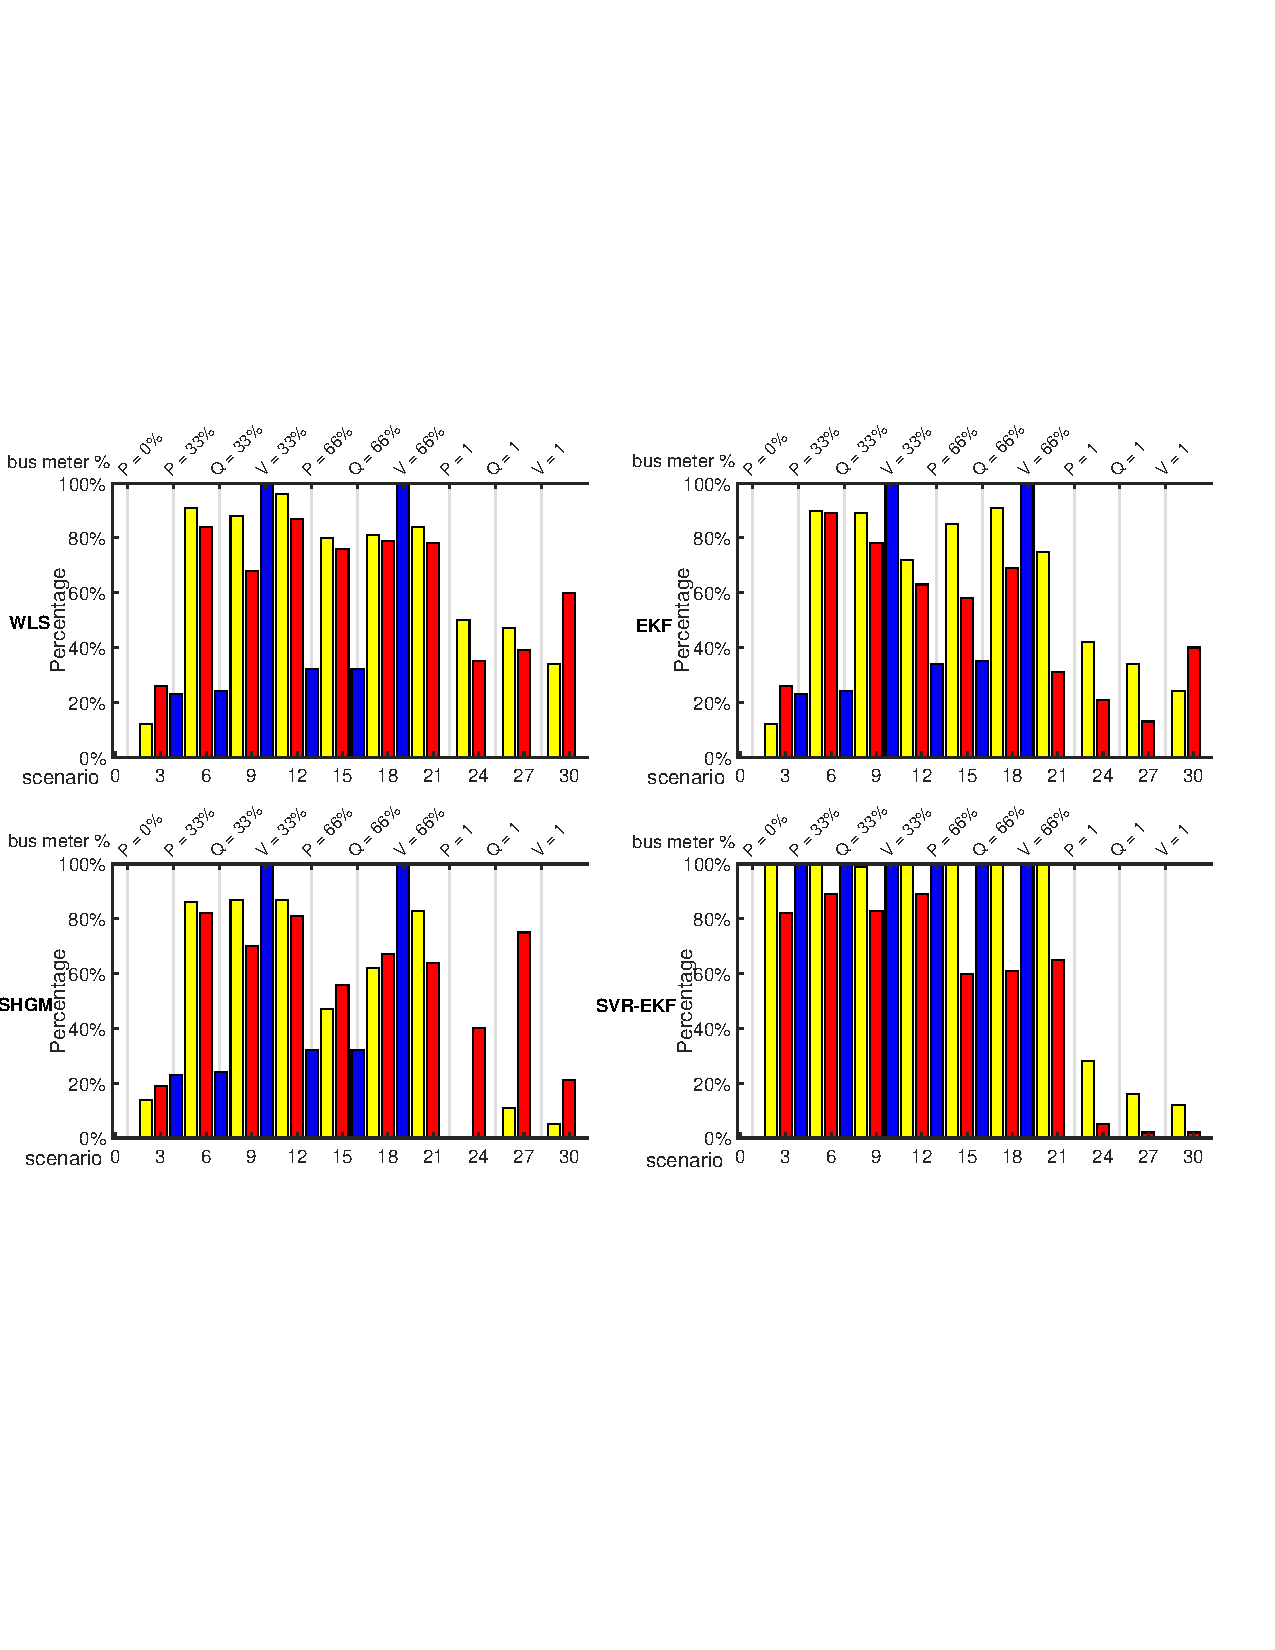
\includegraphics[ height=8cm, width=14cm]{figures/v.pdf}
        \caption{$RMSE^V$ comparison}
        \label{fig:compare_V}
    \end{figure}
The values for scenario 1, 22, 25, and 28 are zero because there is only one possible smart meters location. For WLS, EKF, and SHGM, the proposed smart meters location method can clearly reduce the $RMSE^V$ when the information of the voltage magnitudes is known as shown in scenario 10 and 19, where nearly all of the 100 cases exhibit a higher error than the optimal smart meters location. But the optimality of the smart meters location is not as strong when the level of actual measurements increases. For example, the percentage decreases from scenario 10 to 12 when more branch meters are installed, as well as in the scenarios 23 to 30. As for the SVR-EKF, the mean voltage error is smaller based on the optimal smart meter location method as long as the level of measurements is small. 
\bigskip
\\To conclude, the voltage error can clearly be reduced by using the proposed optimal smart meter location method when the information of voltage magnitudes is known and the level of power flow measurements is low for WLS, EKF, and SHGM. As for SVR-EKF, the performance of the proposed optimal smart meter location selection method slightly decreases when the level of power flow measurements increases.

\subsubsection{Active Power Flow Error}
Figure \ref{fig:compare_P} compares the active power flow error $RMSE^{P_{flow}}$ of the simulation with the optimal smart meters location method with the other 100 cases for each scenario.
    \begin{figure}[!h]
        \centering
        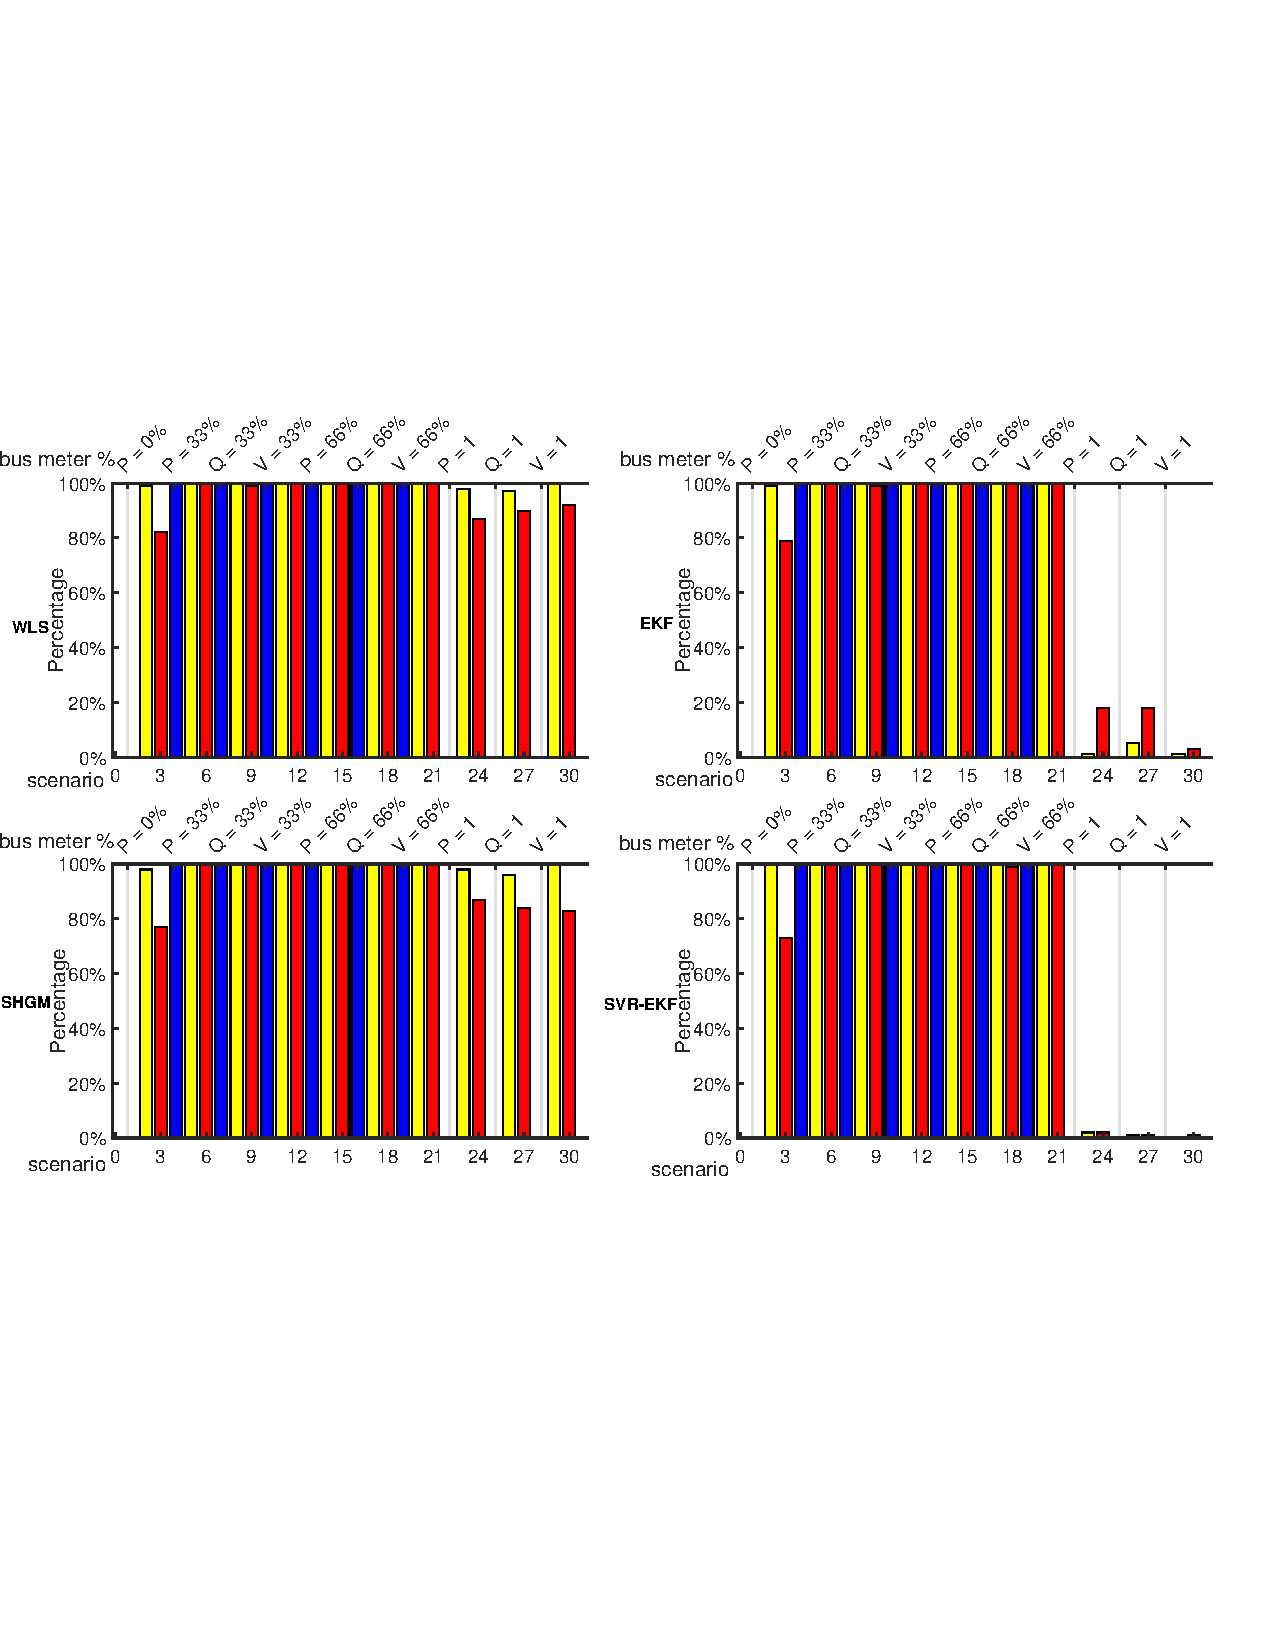
\includegraphics[ height=8cm, width=14cm]{figures/pflow.pdf}
        \caption{$RMSE^{P_{flow}}$ comparison}
        \label{fig:compare_P}
    \end{figure}
For WLS and SHGM, it can be seen that nearly all of the 100 cases show a higher active power flow error than the optimal smart meter location method. But the percentage of 100 cases with a higher $RMSE^{P_{flow}}$ is slightly reduced in scenarios 3, 24, 27, and 30. Scenario 3 shows similar characteristics for all of 4 estimators with a slightly lower percentage. Scenarios 24, 27 and 30 are characterized by a full knowledge of the active power injection and $20 \%$ of power flows measurements. In such conditions, the suggested optimal meter location clearly fails for EKF based algorithms.
    \begin{figure}[!h]
        \centering
        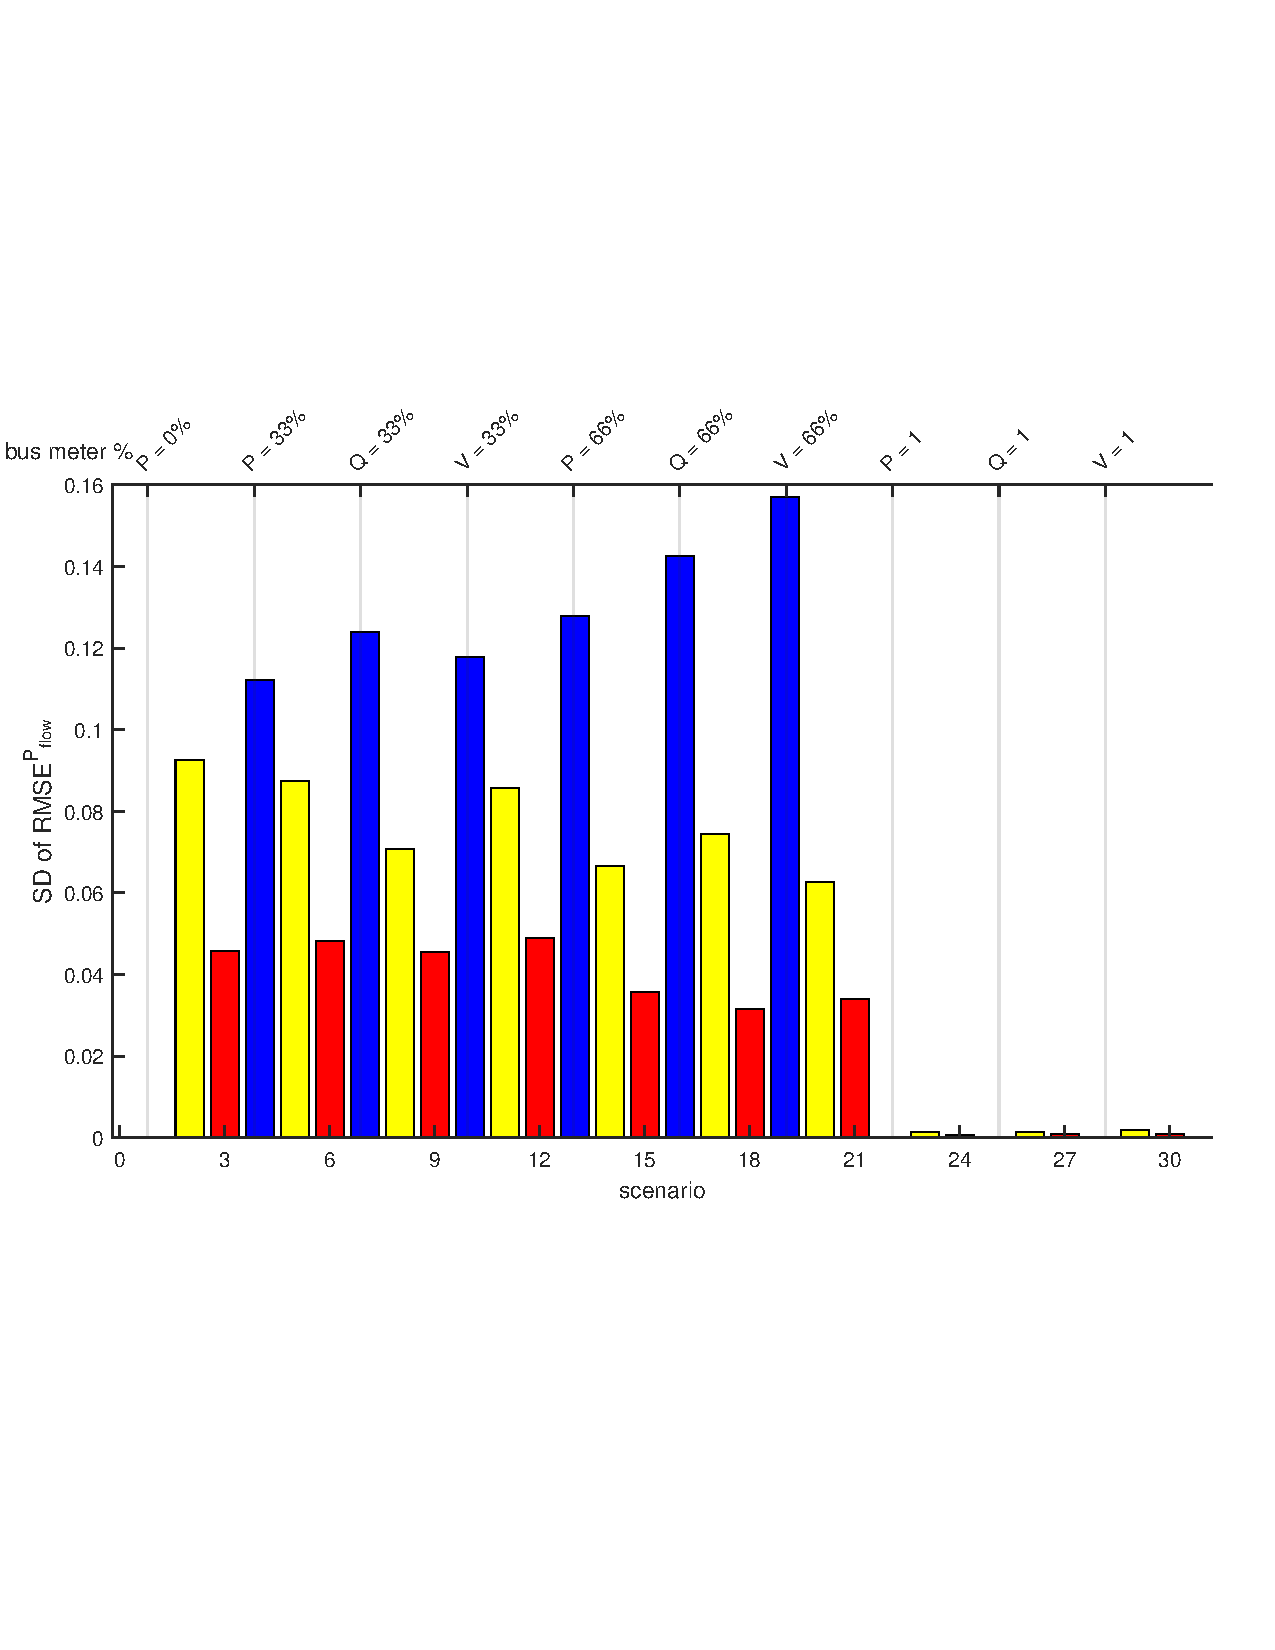
\includegraphics[ height=8cm, width=14cm]{figures/std_pflow.pdf}
        \caption{Standard Deviation of $RMSE^{P_{flow}}$ for WLS}
        \label{fig:std_pflow}
    \end{figure}
This phenomenon can be explained by the Standard Deviation (SD) of $RMSE^{P_{flow}}$ across the 100 cases in each scenario. Figure \ref{fig:std_pflow} shows the SD of $RMSE^{P_{flow}}$ for each scenario with WLS estimator. This figure illustrates the fact that the SD of $RMSE^{P_{flow}}$ is decreasing significantly when the percentage of power flow measurements increases. Also, the SD of $RMSE^{P_{flow}}$ from scenarios 23 to 30 is even close to 0 which indicates that the location of the branch meters almost has no influence on the accuracy of $RMSE^{P_{flow}}$ even though it shows a positive correlation in Spearman' correlation coefficient. As for EKF and SVR-EKF, the suggested optimal location does not contribute to a reduced active power flow error from scenarios 23 to 30 due to the negative Spearman's correlation coefficient $p(RMSE^{P_{flow}},distr^{branch})$.  
\bigskip
\\As a result, the conclusion can be drawn that the proposed optimal smart meter location contributes to a reduced $RMSE^{P_{flow}}$ for the four state estimation algorithms. But this effect gets weaker when the number of branch sensors increases, especially for the scenarios where all the information of active power injection is known and $20 \%$ of the power flow are measured.

\subsubsection{Reactive Power Flow Error}
Similarly to $RMSE^{P_{flow}}$, Figure \ref{fig:compare_Q} shows comparison of the mean reactive power flow error $RMSE^{Q_{flow}}$ between the suggested optimal smart meter locations and the other 100 cases with random smart meter locations for each of the 30 scenarios.
    \begin{figure}[!h]
        \centering
        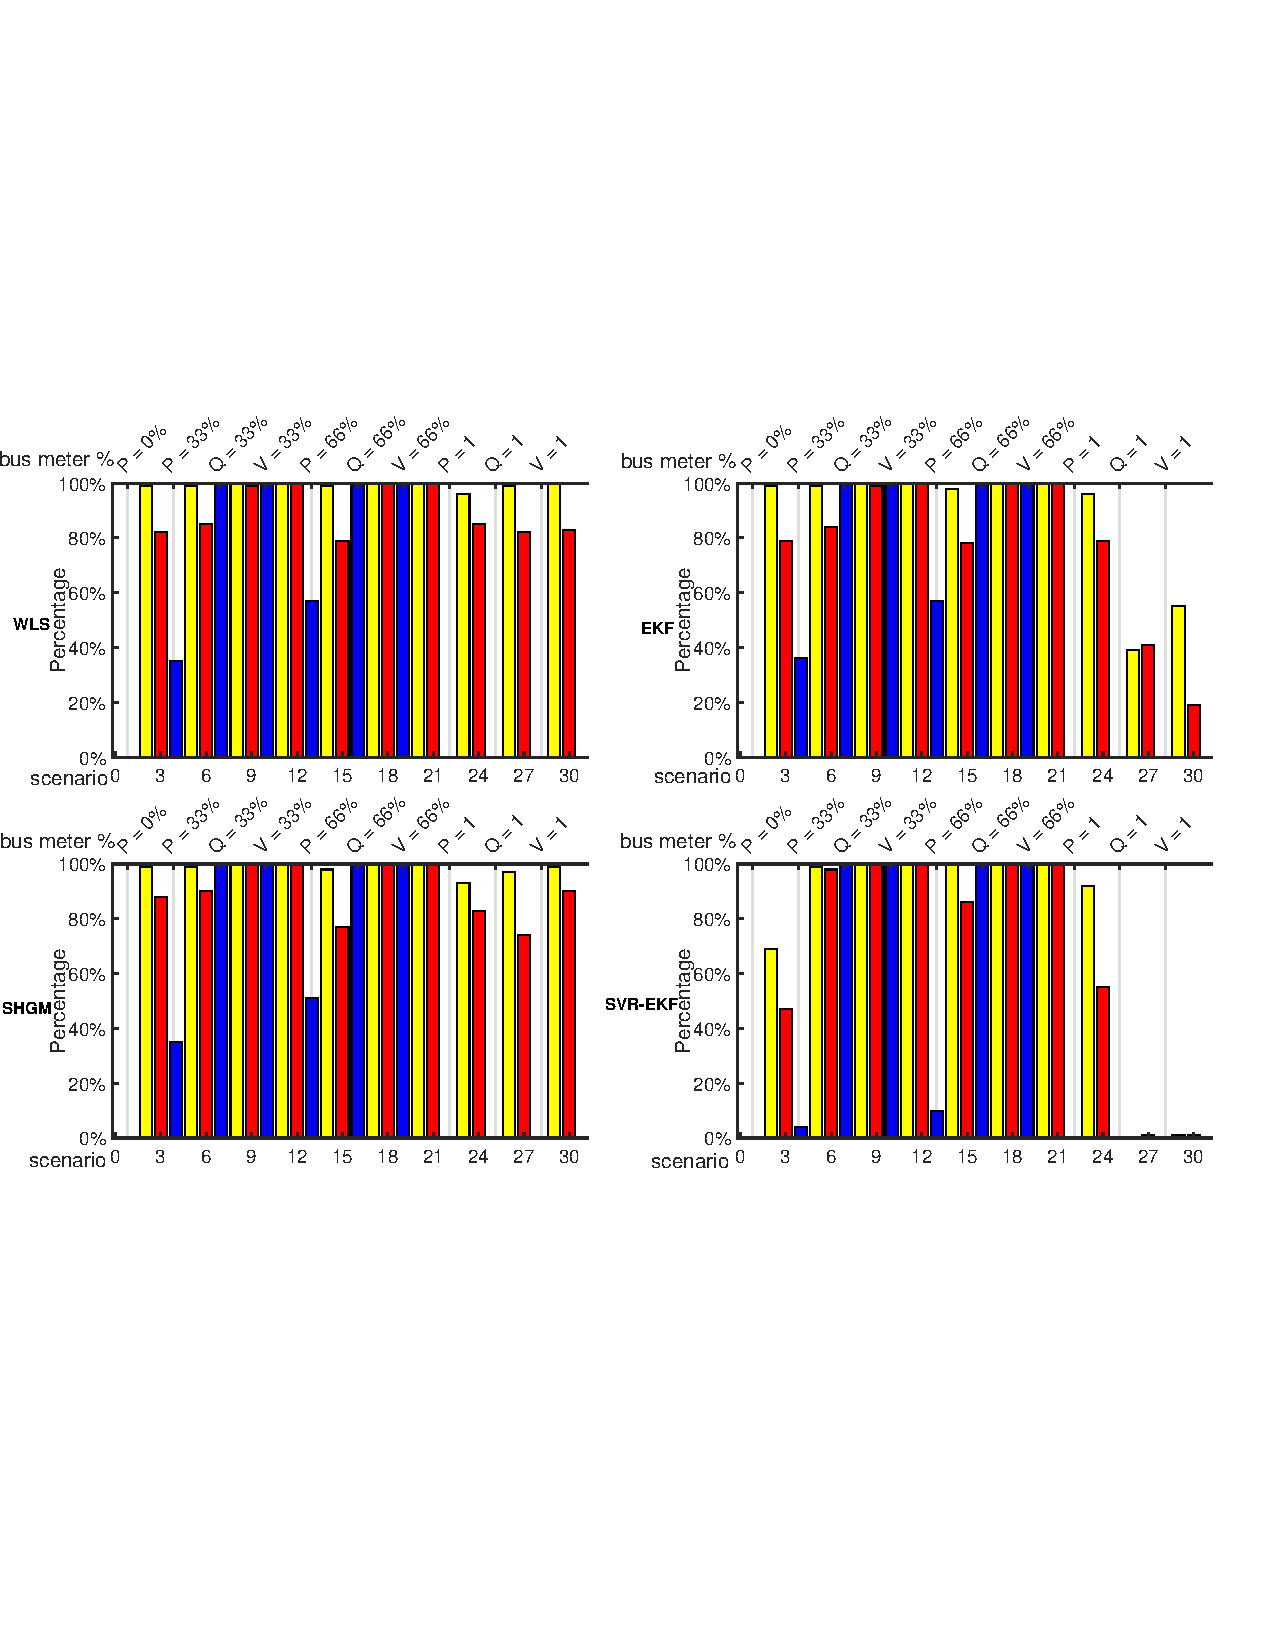
\includegraphics[ height=7cm, width=14cm]{figures/qflow.pdf}
        \caption{$RMSE^{Q_{flow}}$ comparison}
        \label{fig:compare_Q}
    \end{figure}
From scenarios 7 to 12 and 16 to 21, with $33 \%$ and $66\%$ of reactive power measurements, respectively, the suggested optimal meter location outperforms nearly all 100 cases. When $10 \%$ of the power flows are measured , the optimal location is especially good. When the proportion of measured power flow increases from $10 \%$ to $20 \%$, the influence of the branch meters distribution $distr^{branch}$ based on Path Search decreases to approximately $80 \%$ when reactive power injections are not measured as shown in the scenarios with red bars.
\bigskip
\\As for EKF and SVR-EKF, the overall performance is almost the same as WLS and SHGM except scenarios 26 to 30. It can also be explained by the SD of the reactive power flow errors in each scenario. The SD of $RMSE^{Q_{flow}}$ with EKF for 30 scenarios is as shown in Figure \ref{fig:std_qflow}.
    \begin{figure}[!h]
        \centering
        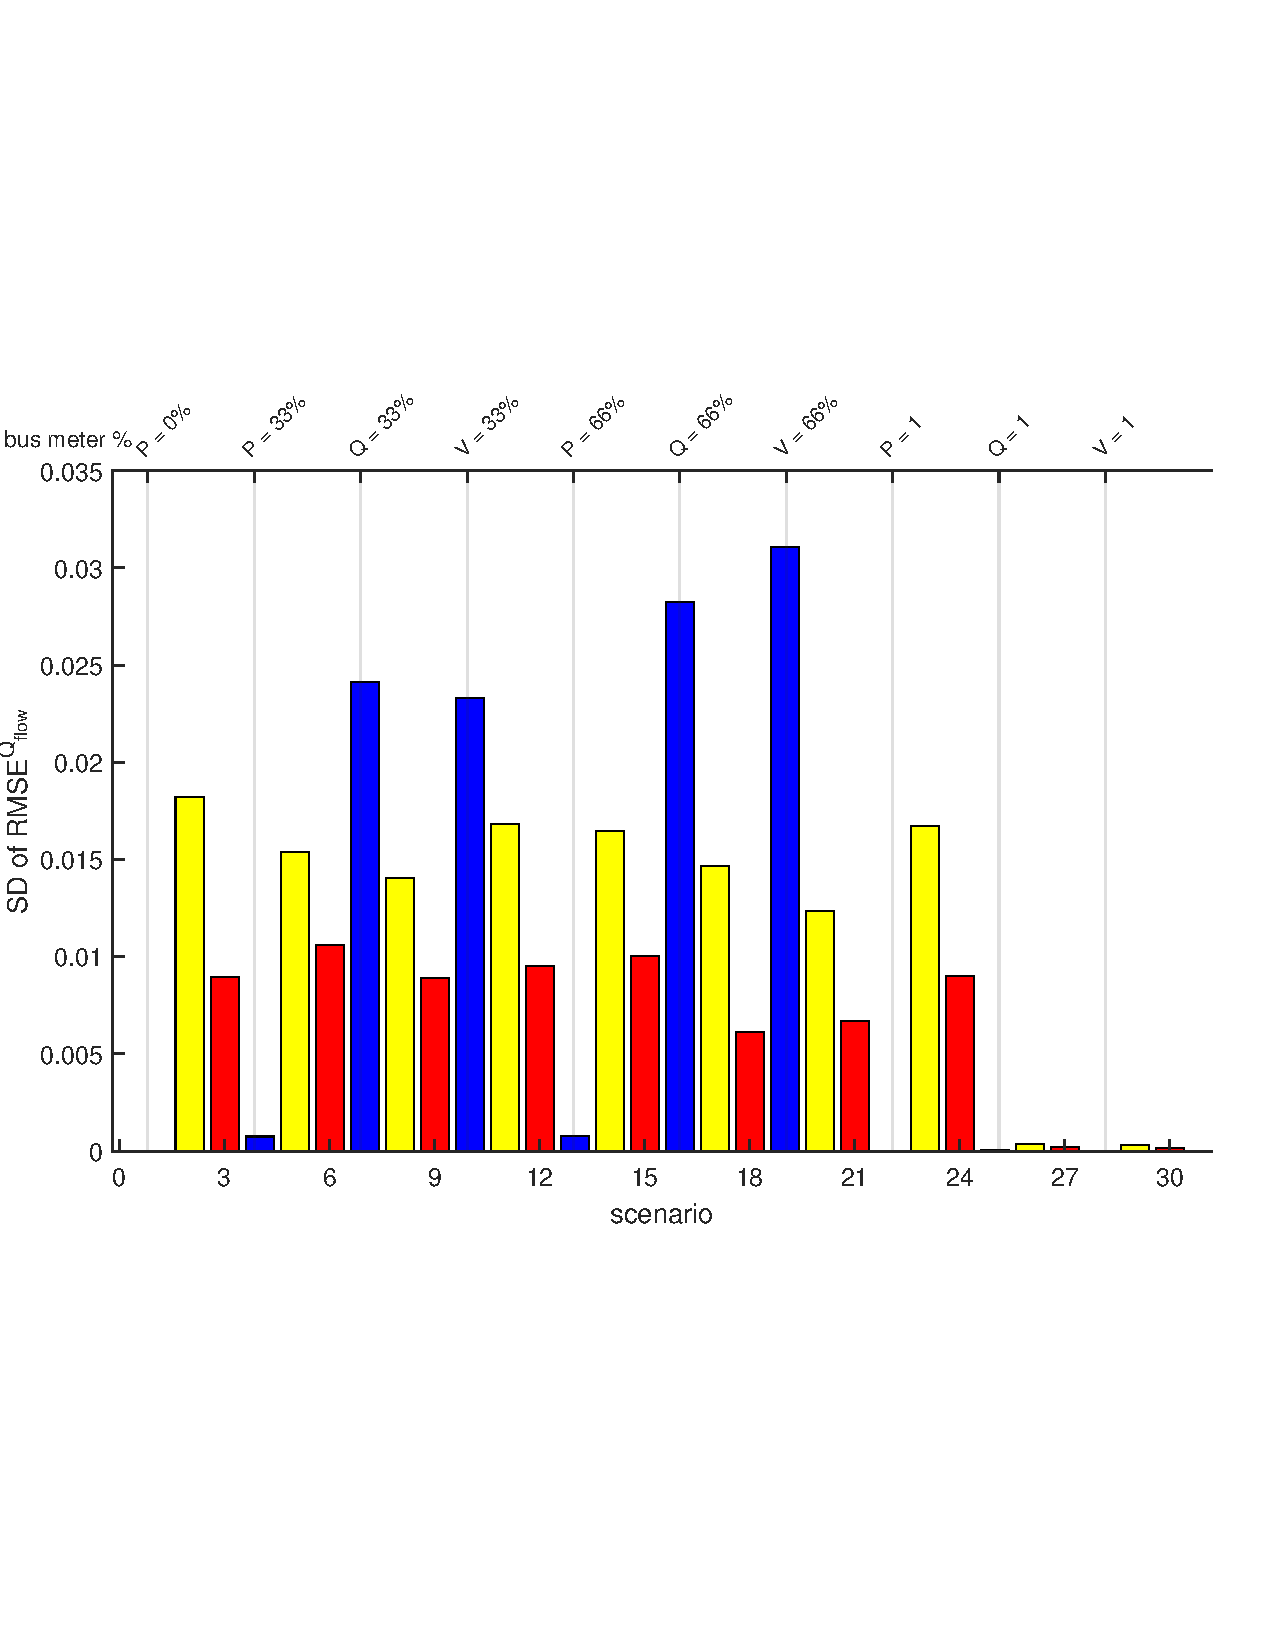
\includegraphics[ height=7cm, width=14cm]{figures/std_qflow.pdf}
        \caption{Standard Deviation of $RMSE^{Q_{flow}}$ for EKF}
        \label{fig:std_qflow}
    \end{figure}
Therefore, the SD in scenarios 26 to 30 are closed to 0 and negligible compared with the other scenarios. Hence, the branch meters distribution based on Path Search almost has no influence on $RMSE^{Q_{flow}}$ in these scenarios.

\subsubsection{Conclusion of the Influence of Smart Meter Location}
 Under the scenarios where the information of voltage magnitudes are known, the mean voltage magnitude error $RMSE^{V}$ can clearly be reduced based on the proposed optimal smart meter location method bus meters are installed at the buses with the highest overall active energy consumption and branch meters are as well distributed as possible based on the Path Search. The active power flow error $RMSE^{P_{flow}}$ can also be reduced, but the optimality of the proposed method is not as strong when many measurements are available such as the scenario where the information of all active power injections is known. The mean reactive power flow error $RMSE^{P_{flow}}$ can also be reduced by the proposed smart meters location method mainly if the information of the reactive power injections is known.

\section{Comparison of Estimators}
In this section, one compares the performance of the implemented four state estimation algorithms with or without the proposed optimal smart meters location method. 
\subsection{Random Smart Meter Location}
Firstly, the performance of the four estimators is compared when the smart meters are installed randomly at the buses and branches based on the 100 Monte-Carlo simulations in each of the 30 scenarios. In a similar way, the mean voltage magnitude error $RMSE^V$, mean active power flow error $RMSE^{P_{flow}}$, and mean reactive power flow error $RMSE^{Q_{flow}}$ is calculated.
\subsubsection{Voltage Magnitude Error}
    \begin{figure}[!h]
        \centering
        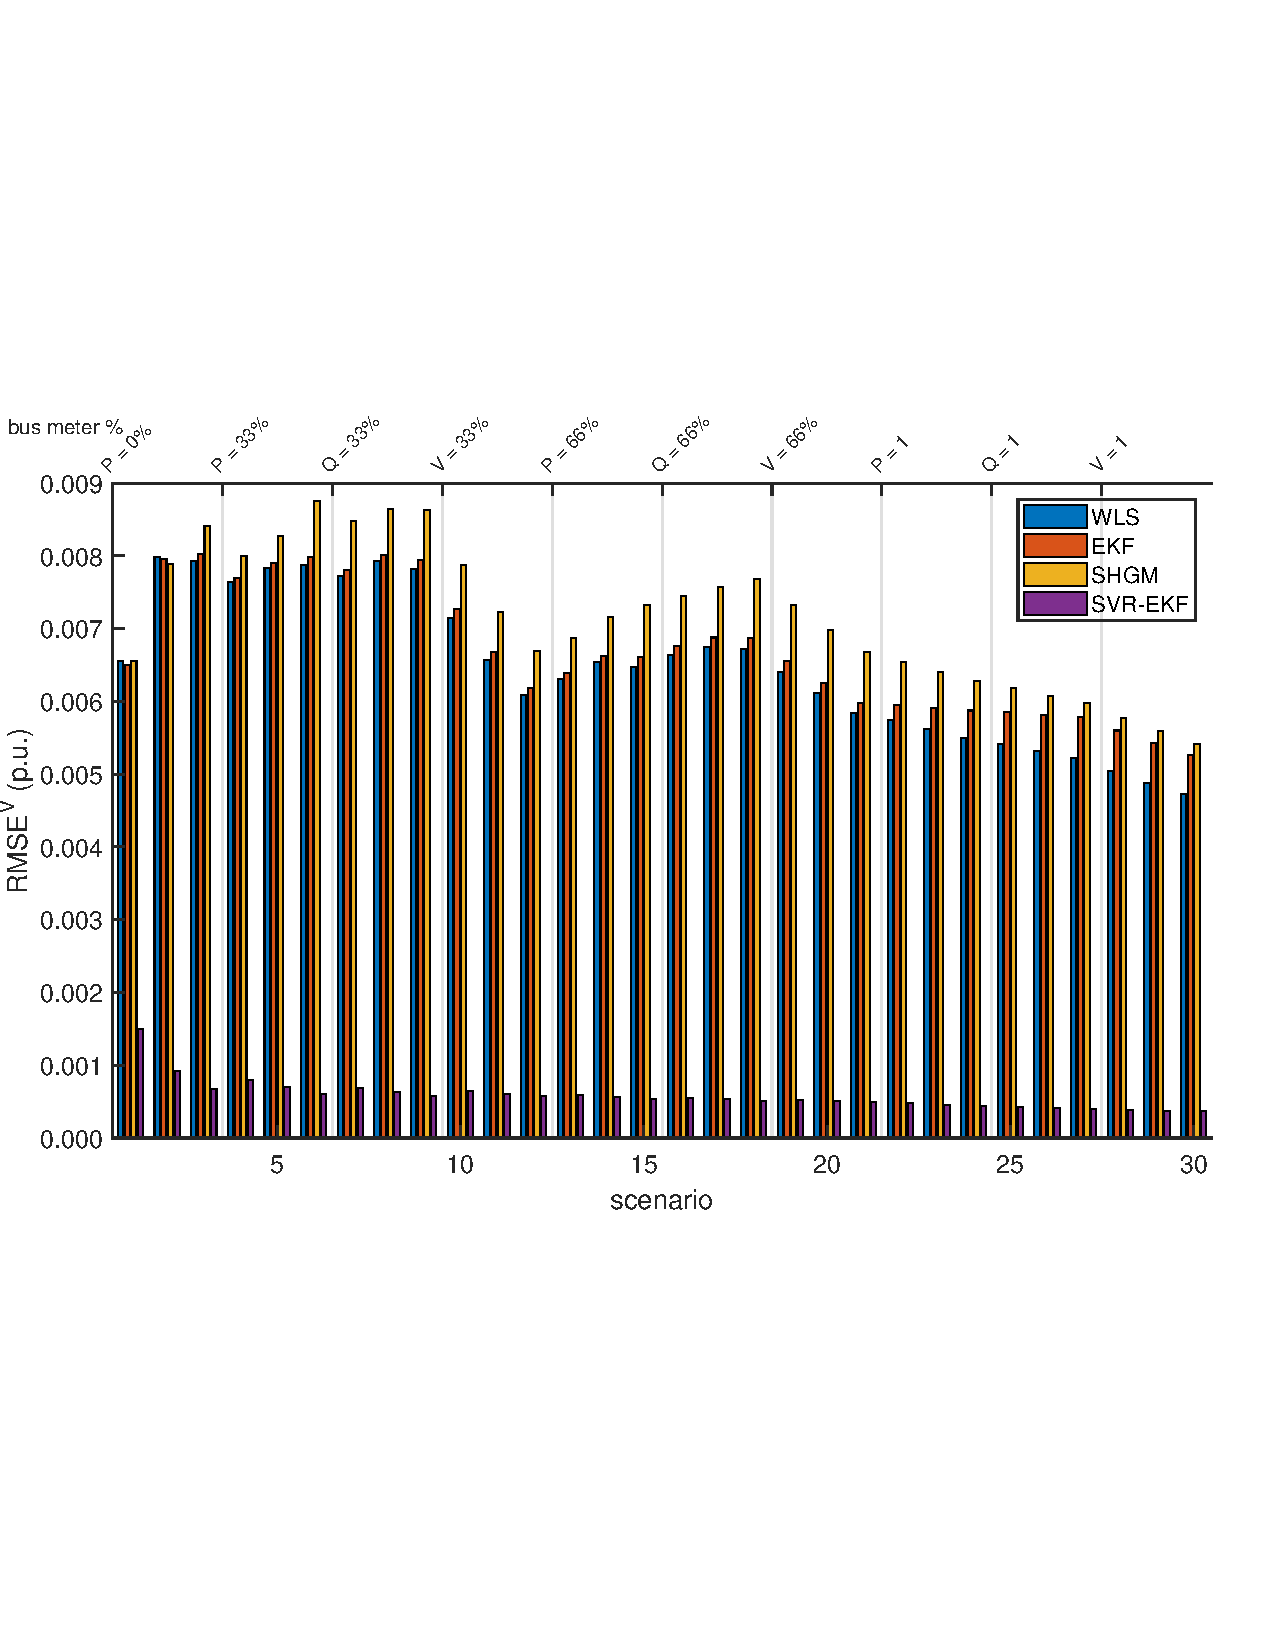
\includegraphics[ height=8cm, width=14cm]{figures/v_100.pdf}
        \caption{Comparison of mean $RMSE^{V}$ for 100 cases}
        \label{fig:v_100}
    \end{figure}
\noindent
Figure \ref{fig:v_100} shows the mean voltage magnitude errors across 100 cases in each of the 30 scenarios for the 4 estimators. It can be seen that SVR-EKF has the smallest voltage in all of the 30 scenarios. In addition, the error monotonously decreases with an increasing number of measurements. The other three algorithms show a significantly higher error, with a small advantage for WLS. For these 3 algorithms, the error generally decreases with an increasing number of measurements. Nevertheless, the error in scenario 1 with no real measurements has a lower value compared with other scenarios. It is because the additional information of the measurements requests the estimated voltage fits the extra measurements information to reduce the power flow and power injection error, which leads to a higher voltage magnitude error. For the same reason,  with $33 \%$ or $66 \%$ of active power injection measurements, the error always increases when adding extra information of the reactive power injections, the active and reactive power flows, and the voltage magnitudes. 

\subsubsection{Active Power Flow Error}
    \begin{figure}[!h]
        \centering
        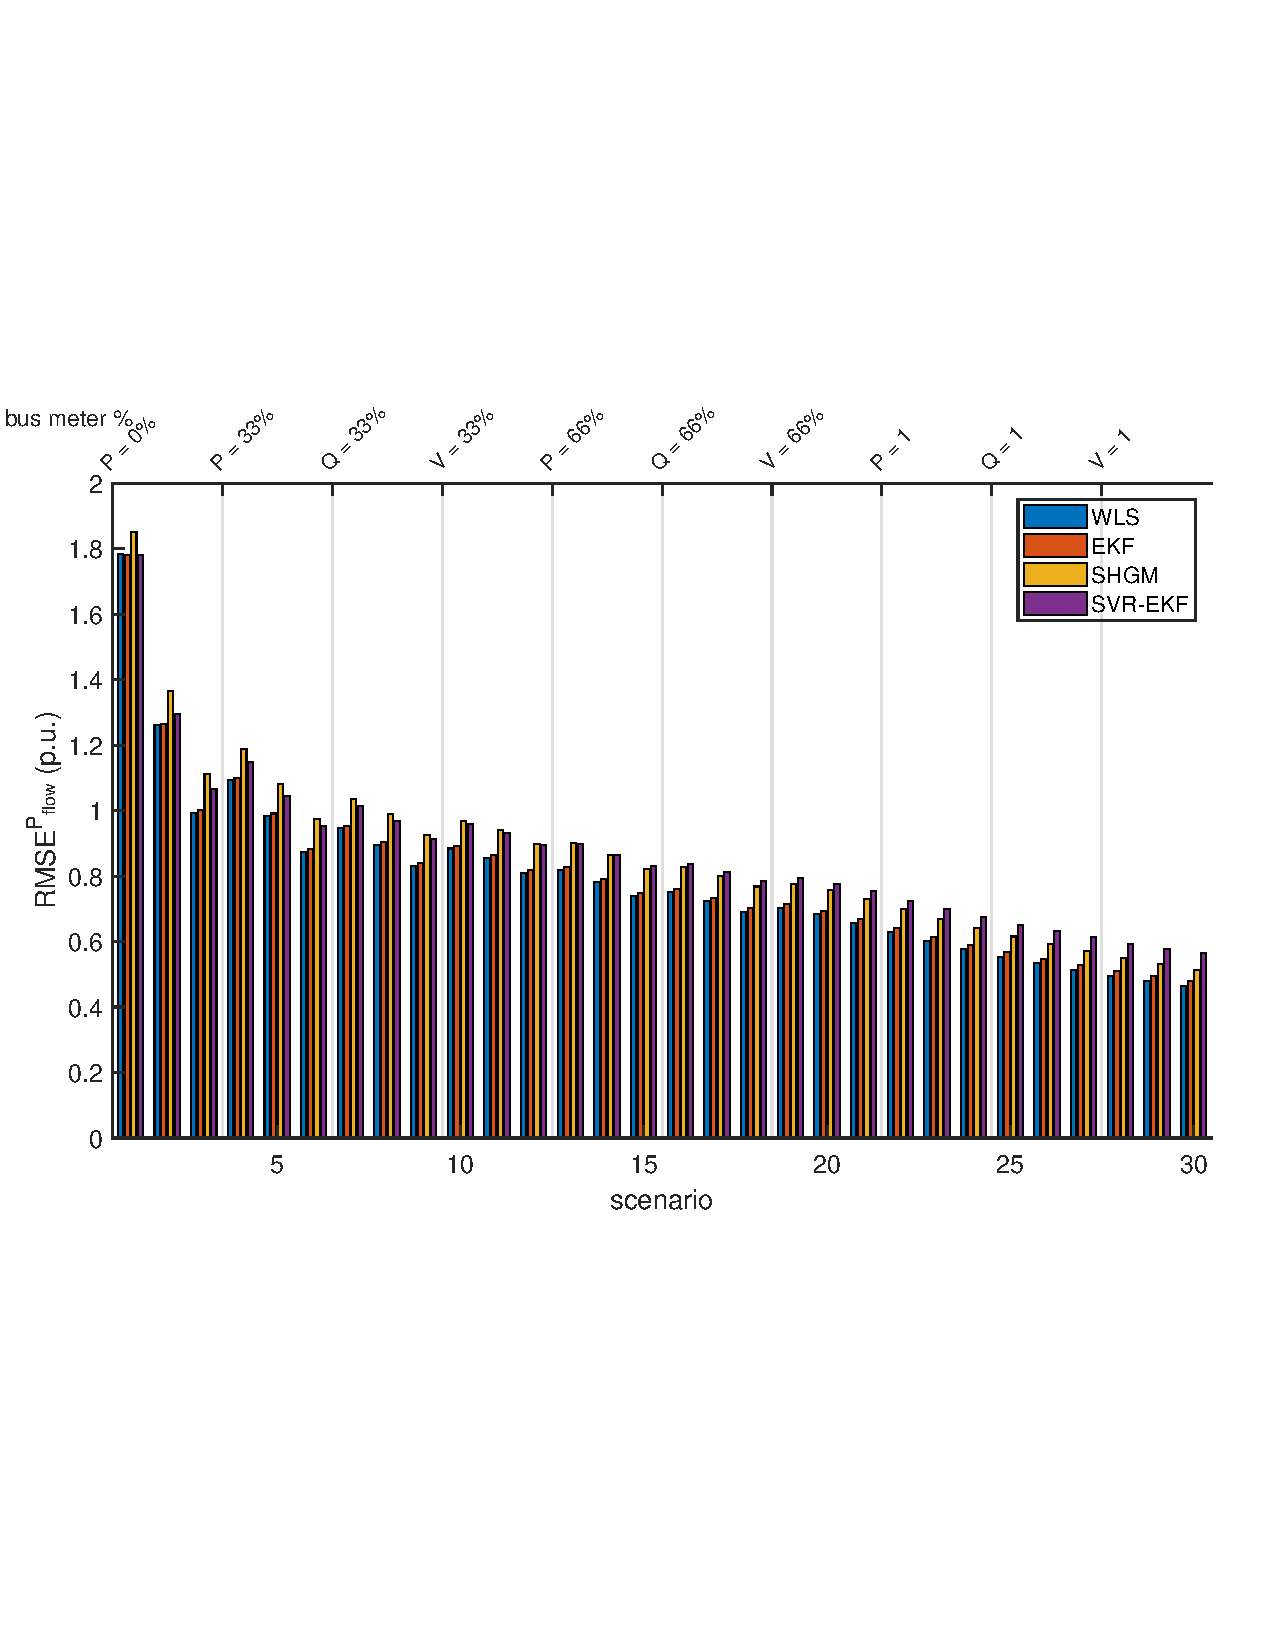
\includegraphics[ height=8cm, width=14cm]{figures/pflow_100.pdf}
        \caption{Comparison of mean $RMSE^{P_{flow}}$ for 100 cases}
        \label{fig:pflow_100}
    \end{figure}
\noindent
The mean active power flow has a more straightforward correlation with the number of measurements as shown in Figure \ref{fig:pflow_100}. WLS has the lowest mean active power flow error $RMSE^{P_{flow}}$ for all of 30 scenarios and EKF has the second smallest one. SHGM has the highest $RMSE^{P_{flow}}$ before scenario 14 whereas SVR-EKF has the highest $RMSE^{P_{flow}}$ from scenario 14 to 30. It is also clear that $RMSE^{P_{flow}}$ is decreasing when the number of measurements increases, and the influence of the branch meters is stronger than the bus meters before scenario 10. For example, when the percentage of the measured power flows increase from $0 \%$ in scenario 1 to $20 \%$ in scenario 3, $RMSE^{P_{flow}}$ decreases from 1.8 to 1 p.u. for WLS. And $RMSE^{P_{flow}}$ decreases by 0.7 from scenario 1 to 4 when the proportion of measured active power injection increases from $0 \%$ to $33 \%$. It is because the number of the measured active power flows in scenario 3 is higher than the number of the measured active power injections in scenario 4, which provides more information and leads to a higher accuracy.
\bigskip
\\In conclusion, WLS has the highest active power flow accuracy for all 30 scenarios. SVR-EKF has the highest active power flow error from scenario 14 on under higher number of measurements and SHGM has the highest $RMSE^{P_{flow}}$ before scenario 14. Nevertheless, the difference in performance between all four algorithms is relatively small.


\subsubsection{Reactive Power Flow Error}
    \begin{figure}[!h]
        \centering
        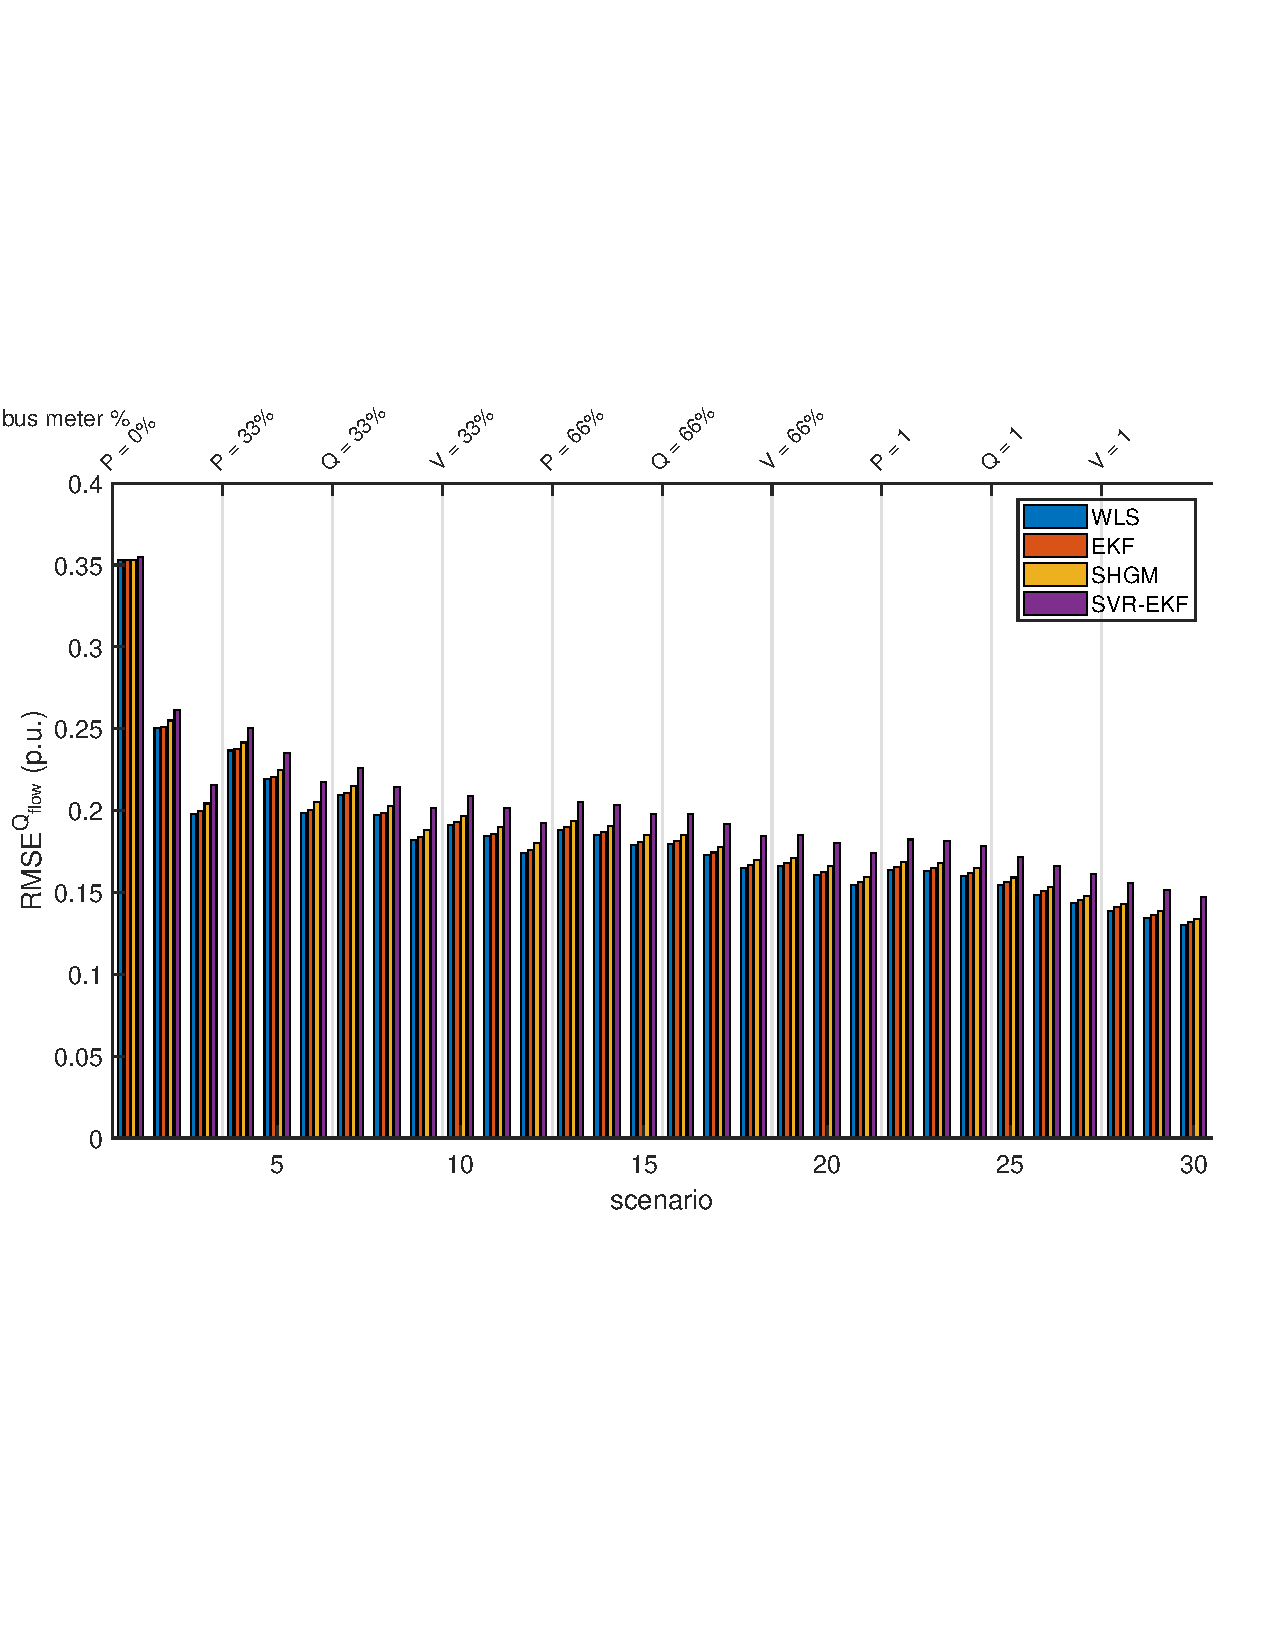
\includegraphics[ height=8cm, width=14cm]{figures/qflow_100.pdf}
        \caption{Comparison of mean $RMSE^{Q_{flow}}$ for 100 cases}
        \label{fig:qflow_100}
    \end{figure}
Similarly, the mean reactive power flow error $RMSE^{Q_{flow}}$ across 100 cases in each scenario for the four estimators is shown in Figure \ref{fig:qflow_100}. WLS has the lowest $RMSE^{Q_{flow}}$ and SVR-EKF has the highest $RMSE^{Q_{flow}}$ in all 30 scenarios. Also, the performance of all these four state estimation algorithms for $RMSE^{Q_{flow}}$ is similar in the scenario 1 without any actual measurements, but this difference is slightly increasing with the increase of the number of measurements. And $RMSE^{Q_{flow}}$ decreases when the percentage of the measured power flow increase such as from scenario 4 to 6, but the strength of the influence of the measured power flow on $RMSE^{Q_{flow}}$ decreases with the increase of measurements redundancy. For example, $RMSE^{Q_{flow}}$ decreases from 0.35 in scenario 1 to 0.2 in scenario 3. But $RMSE^{Q_{flow}}$ only decreases by approximately 0.1 from scenario 4 to 6 for WLS when the measurement redundancy increases. It is because the number of the measured reactive power flows in scenario 3 is higher than the number of the measured reactive power injections in scenario 4, which provides more information and leads to higher accuracy.

\subsubsection{Conclusion}
    \begin{table}[!h]
        \centering
        \begin{tabular}{m{1cm}|m{7cm}|m{7cm}|}
            & \textbf{Advantage} & \textbf{Disadvantage} \\ \hline
            WLS &   \begin{itemize}
                        \item Second smallest voltage magnitude error.
                        \item Smallest active and reactive power flow error.
                    \end{itemize}
                      &   
                    \begin{itemize}
                        \item Higher voltage error than SVR-EKF
                    \end{itemize}
                      \\ \cline{1-3}
            EKF &   \begin{itemize}
                        \item Relatively low error.
                        \item Second lowest computational burden.
                    \end{itemize}
                      &   
                    \begin{itemize}
                        \item Performance depends on the parameters.
                    \end{itemize}
                      \\ \cline{1-3}
            SHGM &   \begin{itemize}
                        \item Identify the leverage points.
                    \end{itemize}
                      &   
                    \begin{itemize}
                        \item Highest error.
                        \item Relatively high computational burden.
                    \end{itemize}
                      \\ \cline{1-3} 
            SVR-EKF &   \begin{itemize}
                        \item Smallest voltage magnitude error.
                    \end{itemize}
                      &   
                    \begin{itemize}
                        \item High power flow error.
                        \item Highest computational burden.
                    \end{itemize}
                      \\ \cline{1-3}                       
        \end{tabular}
        \caption{Comparison of estimators with random smart meter location}
        \label{tab:compare_4_table}
    \end{table}
Based on the simulations and analysis shown above, the advantages and disadvantages of each state estimation algorithms are listed in Table \ref{tab:compare_4_table}. If low voltage magnitude is desired by DSO, SVR-EKF can be used with the disadvantage that it brings high active and reactive power flow error. SHGM is not suitable for the distribution grid because nearly all of the measurements are defined as leverage points which brings high estimation errors. WLS is the most robust algorithm for the distribution grid which provides acceptable accuracy on both voltage magnitude and power flows.   

\subsection{Optimal Smart Meter Location}
This section compares the performance of the four estimators by installing the smart meters at the optimal locations proposed in Section \ref{sec:analysis_meter_location}. Notice that only scenarios 1 to 21 are compared due to the fact the Spearman's correlation coefficients $p(RMSE^{P_{flow}},dist^{branch})$ between active power flow error and distribution of the branch meters based on Path Search or $p(RMSE^{Q_{flow}},dist^{branch})$ between reactive power flow error and distribution of the branch meters based on Path Search are negative from scenario 21 to 30 for EKF and SVR-EKF, which makes the problem more complex. As a reminder, bus meters are suggested to be installed at buses with high active energy consumption and branch meters as well distributed as possible based on Path Search. 

\subsubsection{Voltage Magnitude Error}
    \begin{figure}[!h]
        \centering
        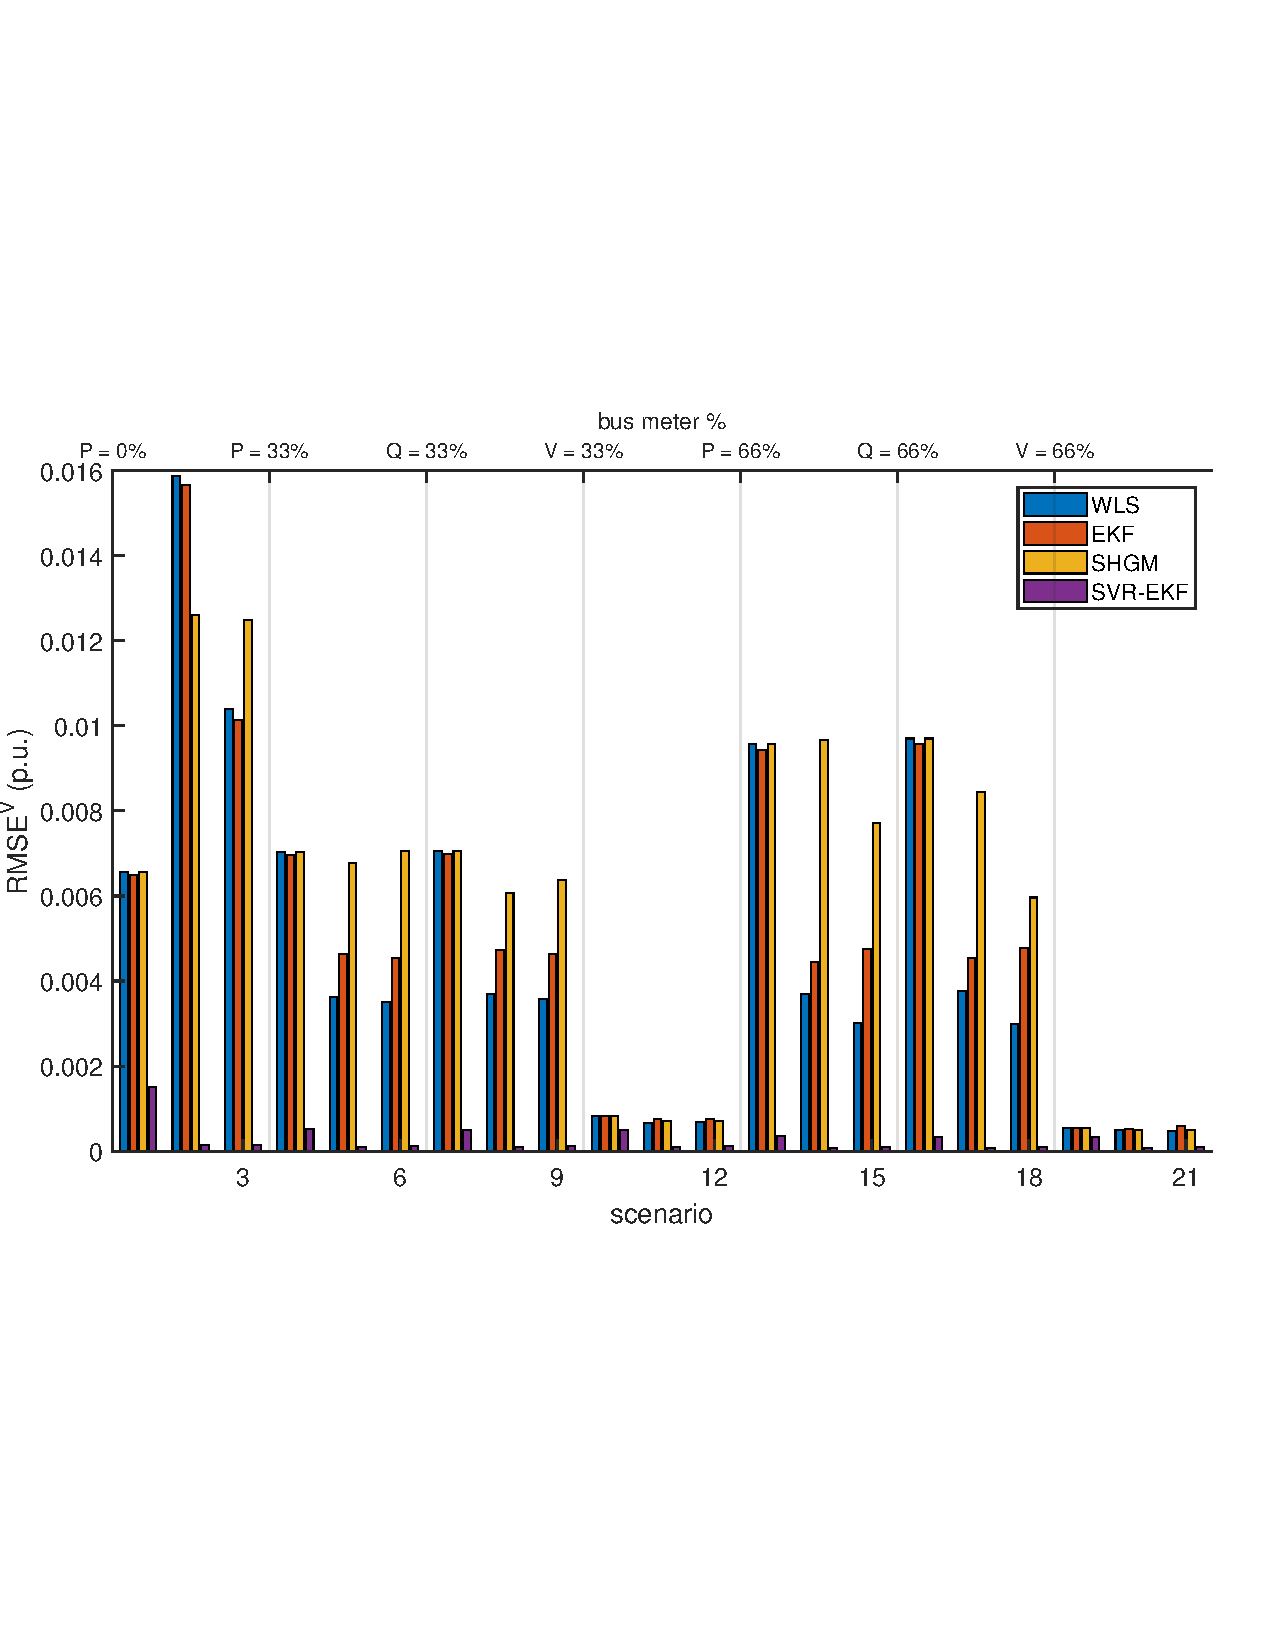
\includegraphics[ height=8cm, width=14cm]{figures/v_op.pdf}
        \caption{Comparison of $RMSE^{V}$ for 4 estimators under optimal meter location}
        \label{fig:v_op}
    \end{figure}
\noindent
The voltage magnitude errors are compared for the 4 estimators under optimal smart meter location, and the result is shown in Figure \ref{fig:v_op}. Similarly to the situation where smart meters are installed randomly, SVR-EKF definitely leads to the smallest error in all 21 scenarios and SHGM has the highest $RMSE^V$ for most of the scenarios such as scenarios 5 to 9. The voltage magnitude errors can be reduced significantly by increasing the number of voltage magnitude measurements as shown in Figure \ref{fig:v_op}. Nevertheless, the error in scenario 1 with no real measurements has a lower value compared with scenarios 2 and 3 which brings additional power flows information. It is because the additional information of the power flow measurements requests the estimated voltage fits the extra power flows measurements to reduce the power flow error, which leads to a higher voltage magnitude error. However, the voltage magnitude errors can be reduced by increasing the number of the power flows measurements under scenarios 4 to 30. 
\bigskip
\\Compared to the mean voltage magnitude error for 100 cases with random smart meter location in Figure \ref{fig:v_100}, the $RMSE^V$ values of SVR-EKF are reduced for all 21 scenarios. Especially under the scenarios where the voltage magnitude information is known, the $RMSE^V$ with optimal smart meter location is significantly smaller compared to the random smart meters location for all four estimators. For example, the $RMSE^V$ for WLS in scenario 10 with random smart meter location is approximately 0.007 whereas the value of $RMSE^V$ in scenario 10 is only 0.0008 with optimal smart meter location method. As for the other scenarios, with the proposed optimal smart meter location, $RMSE^V$ can be reduced when the information of power flow in known, which is reasonable since the voltage magnitude errors in scenarios with more information of the power flows are smaller as shown in Figure \ref{fig:v_op}.

\subsubsection{Active Power Flow Error}
    \begin{figure}[!h]
        \centering
        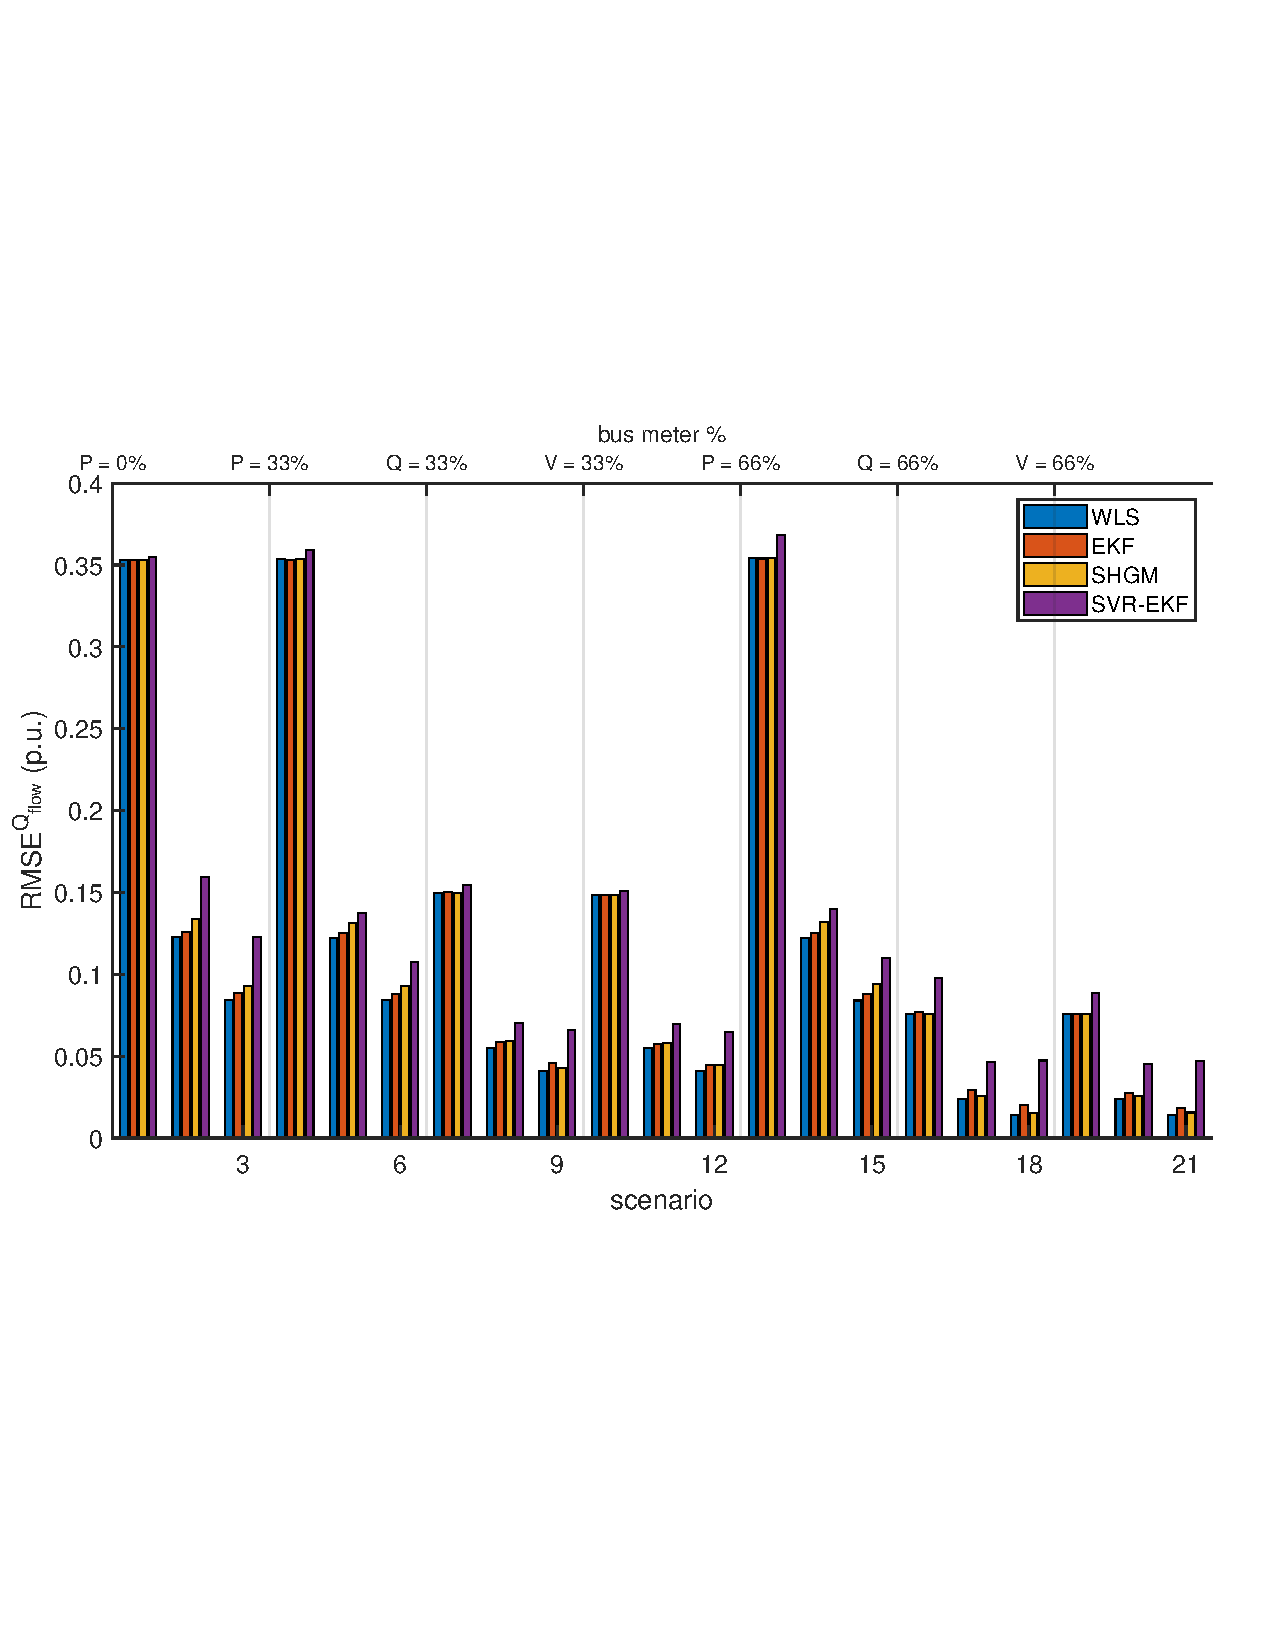
\includegraphics[ height=8cm, width=14cm]{figures/pflow_op.pdf}
        \caption{Comparison of $RMSE^{P_{flow}}$ for 4 estimators under optimal meter location}
        \label{fig:pflow_op}
    \end{figure}
\noindent
As for the active power flow errors, information about reactive power injections or voltage magnitudes almost has no influence on the accuracy of active power flows for all these four estimators. For example, when there is no power flow measurement in scenario 4, 7, and 10, the $RMSE^{P_{flow}}$ is almost the same even though more reactive power injections and voltage magnitudes are measured. The percentage of measured power flows have a strong influence on $RMSE^{P_{flow}}$, especially when the percentage increases from $0 \%$ to $10 \%$, which nearly decrease the error by half.
\bigskip
\\Compared to the situation with random smart meters location as shown in Figure \ref{fig:pflow_100}, the $RMSE^{P_{flow}}$ for all 21 scenarios with four estimators are smaller under the optimal smart meter location, especially under the scenarios with power flow measurements. For example, $RMSE^{P_{flow}}$ is 0.3 for WLS in scenario 5 under optimal meter location which is decreased by 0.7 compared to the random smart meter location. For all 21 scenarios shown in Figure \ref{fig:pflow_op} under optimal smart meter location, WLS has the lowest $RMSE^{P_{flow}}$. SHGM has the highest $RMSE^{P_{flow}}$ before scenario 2 and SVR-EKF has the highest $RMSE^{P_{flow}}$ from scenario 3 to 21.

\subsubsection{Reactive Power Flow Error}
    \begin{figure}[!h]
        \centering
        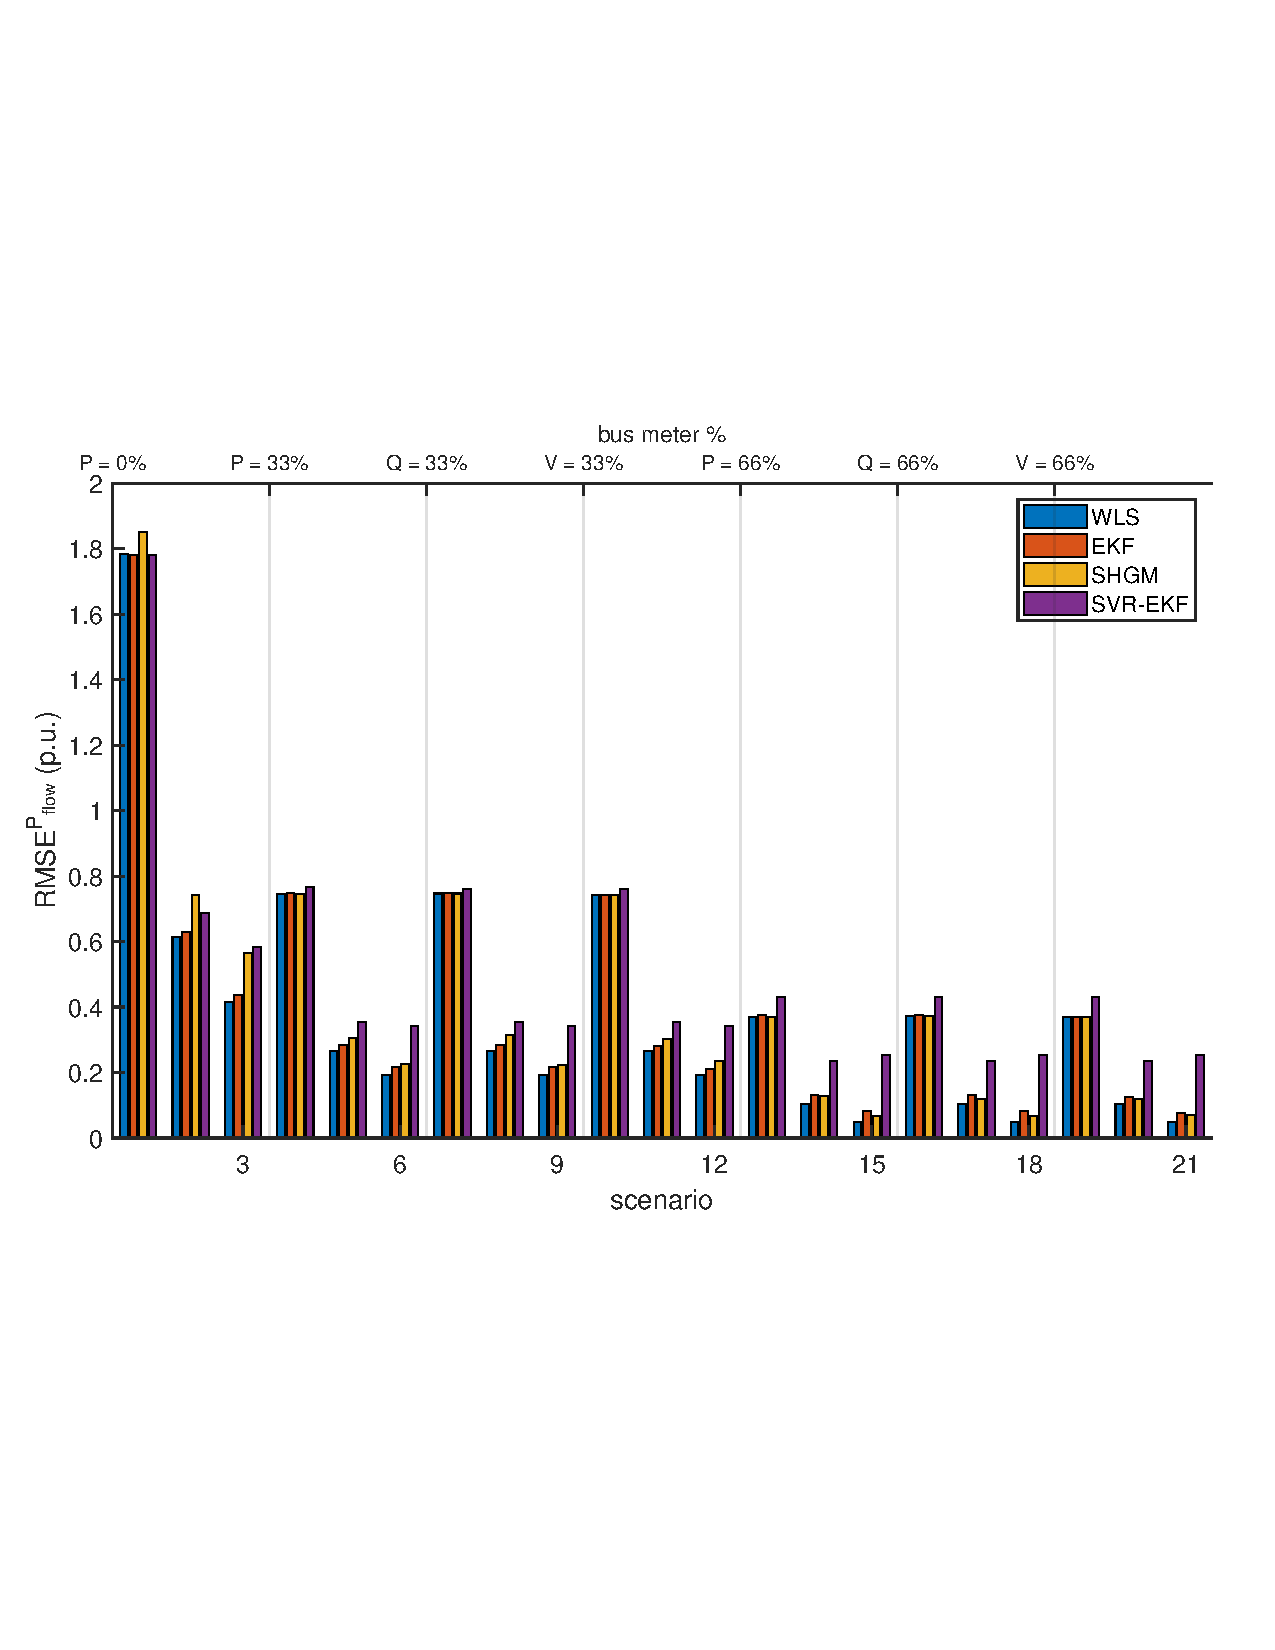
\includegraphics[ height=8cm, width=14cm]{figures/qflow_op.pdf}
        \caption{Comparison of $RMSE^{Q_{flow}}$ for 4 estimators under optimal meter location}
        \label{fig:qflow_op}
    \end{figure}
\noindent
Figure \ref{fig:qflow_op} shows the reactive power flow error $RMSE^{Q_{flow}}$ for 21 scenarios under optimal smart meter location. It can be seen that the $RMSE^{Q_{flow}}$ does not decrease when the number of measured active power injections or voltage magnitudes increases, such as the $RMSE^{Q_{flow}}$ in scenario 1, 4 and 13 whose $RMSE^{Q_{flow}}$ are almost at the same level with the increase of measured active power injection. But $RMSE^{Q_{flow}}$ can be decreased dramatically when the number of measured reactive power injection or reactive power flow increases. For example, $RMSE^{Q_{flow}}$ decreased from 0.35 in scenario 4 without reactive power injection information to 0.15 with $33 \%$ measured reactive power injection.
\bigskip
\\Compared to the scenarios with random smart meter location in Figure \ref{fig:qflow_100}, the $RMSE^{Q_{flow}}$ based on optimal smart meter location can be reduced when the information of the reactive power injection or reactive power flow is known. However, the $RMSE^{Q_{flow}}$ under optimal smart meter location are larger under scenarios without reactive power injection or flow measurements. For instance in scenario 4, there is an error of 0.35 under the suggested optimal meter location and an error of 0.25 with random meter location. And the reason is that the suggested optimal meter location method can reduce the reactive power flow error only if there are smart meters measuring the reactive power injections or power flows.

\subsubsection{Conclusion}
By comparing the estimation result between the random smart meter location and optimal smart meter location, the following conclusions can be drawn:
\begin{itemize}
    \item The derived optimal smart meter location method can reduce the voltage magnitude error $RMSE^V$ under the scenario whose information of voltage magnitude or power flow is known.
    \item The derived optimal smart meter location method can reduce the mean active power flow error $RMSE^{P_{flow}}$ under all of the 21 situation.
    \item The derived smart meter location selection method can reduce the mean reactive power flow error $RMSE^{Q_{flow}}$ under the scenario whose information of reactive power injection or reactive power flow is known.
\end{itemize}



%6 Conclusions and Outlook
\chapter{Conclusion and Outlook}

\section{Conclusion}
In this thesis, four state estimation algorithms, namely WLS, EKF, SHGM, and a newly developed estimator called SVR-EKF, are implemented and tested on one balanced IEEE low voltage distribution grid with radial structure and 206 buses. The grid is populated with household loads and PV generators from the City of Basel. After running power flow calculation based on the given load, the benchmark case is created, where power flows and voltages are notably simulated. From this point on, only a part of the active and reactive power injections, power flows and voltages are assumed to be actually measured, depending on the scenario to consider. In order to simulate a realistic situation, noise is added to the measurements. After adding pseudo-measurements at the buses without measurements of active or reactive power injection to ensure system observability, the state estimation algorithms are tested on 30 scenarios with different level and types of measurements. Each scenario consists of 100 cases with a different location of bus meters and branch meters. By comparing the voltage magnitude error $RMSE^{V}$, the active power flow error $RMSE^{P_{flow}}$, and the reactive power flow error $RMSE^{Q_{flow}}$, at all 206 buses, the result shows that SVR-EKF has the highest voltage magnitude accuracy but also leads to high active and reactive power flow error. SHGM has the worst performance over the four estimators in the distribution grid due to the high level of measurements identified as leverage points. WLS is the best estimator for the radial distribution grid, having the smallest active and reactive power flow errors and the second smallest voltage magnitude error. In general, bad pseudo-measurements of active power injection have the most significant negative impact on the cost function of the state estimators.
\bigskip
\\By neglecting the interaction between bus meters and branch meters, the influence of the location of different meters on the accuracy of estimators has been investigated based on their distance to the feeder bus and their distribution across the entire grid. The result shows that the distance of the smart meters to the feeder bus has no influence on the accuracy of estimators, however the distribution of branch meters based on Path Search has an effect on the accuracy of active and reactive power flows, which can be reduced if they are well distributed across the grid. In addition, active and reactive power flow errors can be reduced by installing the smart meters at the buses with high overall active energy consumption. Hence, an optimal bus and branch meter location has been suggested based on these empirical outcomes.
\bigskip
\\After comparing the simulation with proposed optimal smart meter location and other 100 cases with random smart meter location, the proposed optimal method can reduce voltage magnitude errors when there are meters measuring the voltage magnitude or power flows. The active power flow error can be decreased dramatically by using the proposed meter location strategy. The reactive power flow error can be reduced under the proposed optimal meter location only if the reactive power injections are measured by bus meters or reactive power flows are measured by branch meters.



\section{Outlook}
On the basis of this thesis, further work can be carried out. Some possible research directions are:
\begin{itemize}
    \item The structure of the tested distribution grid in this project is radial, another meshed grid could also be tested for determining if the proposed optimal meter location method still applies for other grid structures.
    \item The tested distribution system is assumed to be balanced. But the distribution grid is usually unbalanced in reality. An unbalanced distribution grid could also be tested.
    \item In the proposed SVR-EKF state estimation algorithm, SVR is used for estimating the voltage magnitude of each bus and EKF is utilized for estimating the voltage phased angle of each bus. If only voltage magnitude, active and reactive power flow are desired by DSO, the EKF can be totally replaced by SVR for directly estimating the desired quantities.
    \item For simplification, bus and branch meters are assumed to work independently. The actual interaction between bus meters, branch meters, and virtual measurements should be considered in a future work.
    \item In this work, the proposed optimal meter location for each scenario of measurement penetration has been compared to 100 analog cases with random meter location obtained by Monte-Carlo simulation. In future work, an optimization problem could be formulated in order to actually find the optimal placement of the different meters assuming that their number is fixed.
    \item For simplification, a constant power factor is assumed for the residential consumers to obtain the reactive power injections, which is not totally realistic. In future work, actual reactive power injections should be collected and used for the simulation.

\end{itemize}





\newpage



%Appendix
\begin{appendices}

\chapter{Correlation Coefficient}

\section{Spearman Coefficient}
\subsection{Bus Meters Distance to the Feeder Bus}
    \begin{figure}[!htb]
        \centering
        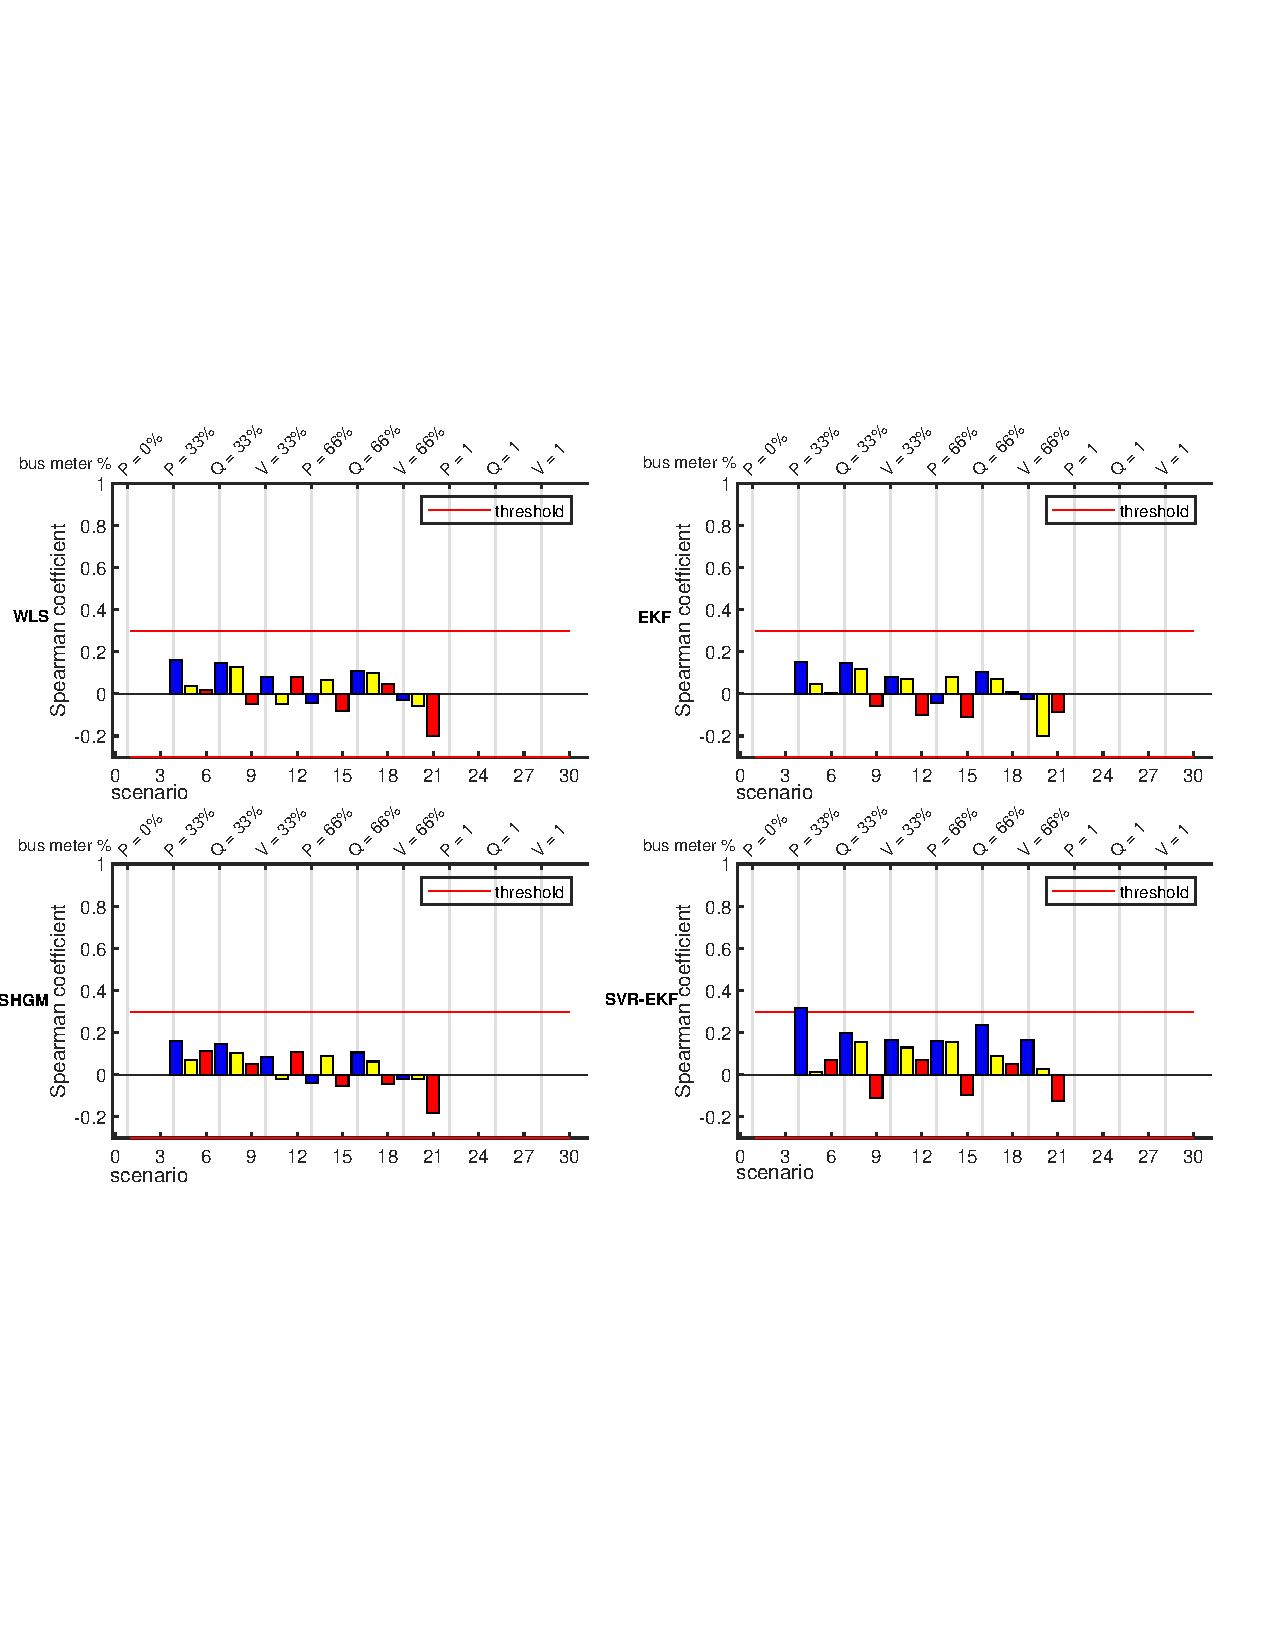
\includegraphics[ height=8cm, width=14cm]{figures/appendix/spearman_bus_meter_V.pdf}
        \caption{Spearman coefficient $p(RMSE^V,dist^{bus})$}
    \end{figure}

    \begin{figure}[!htb]
        \centering
        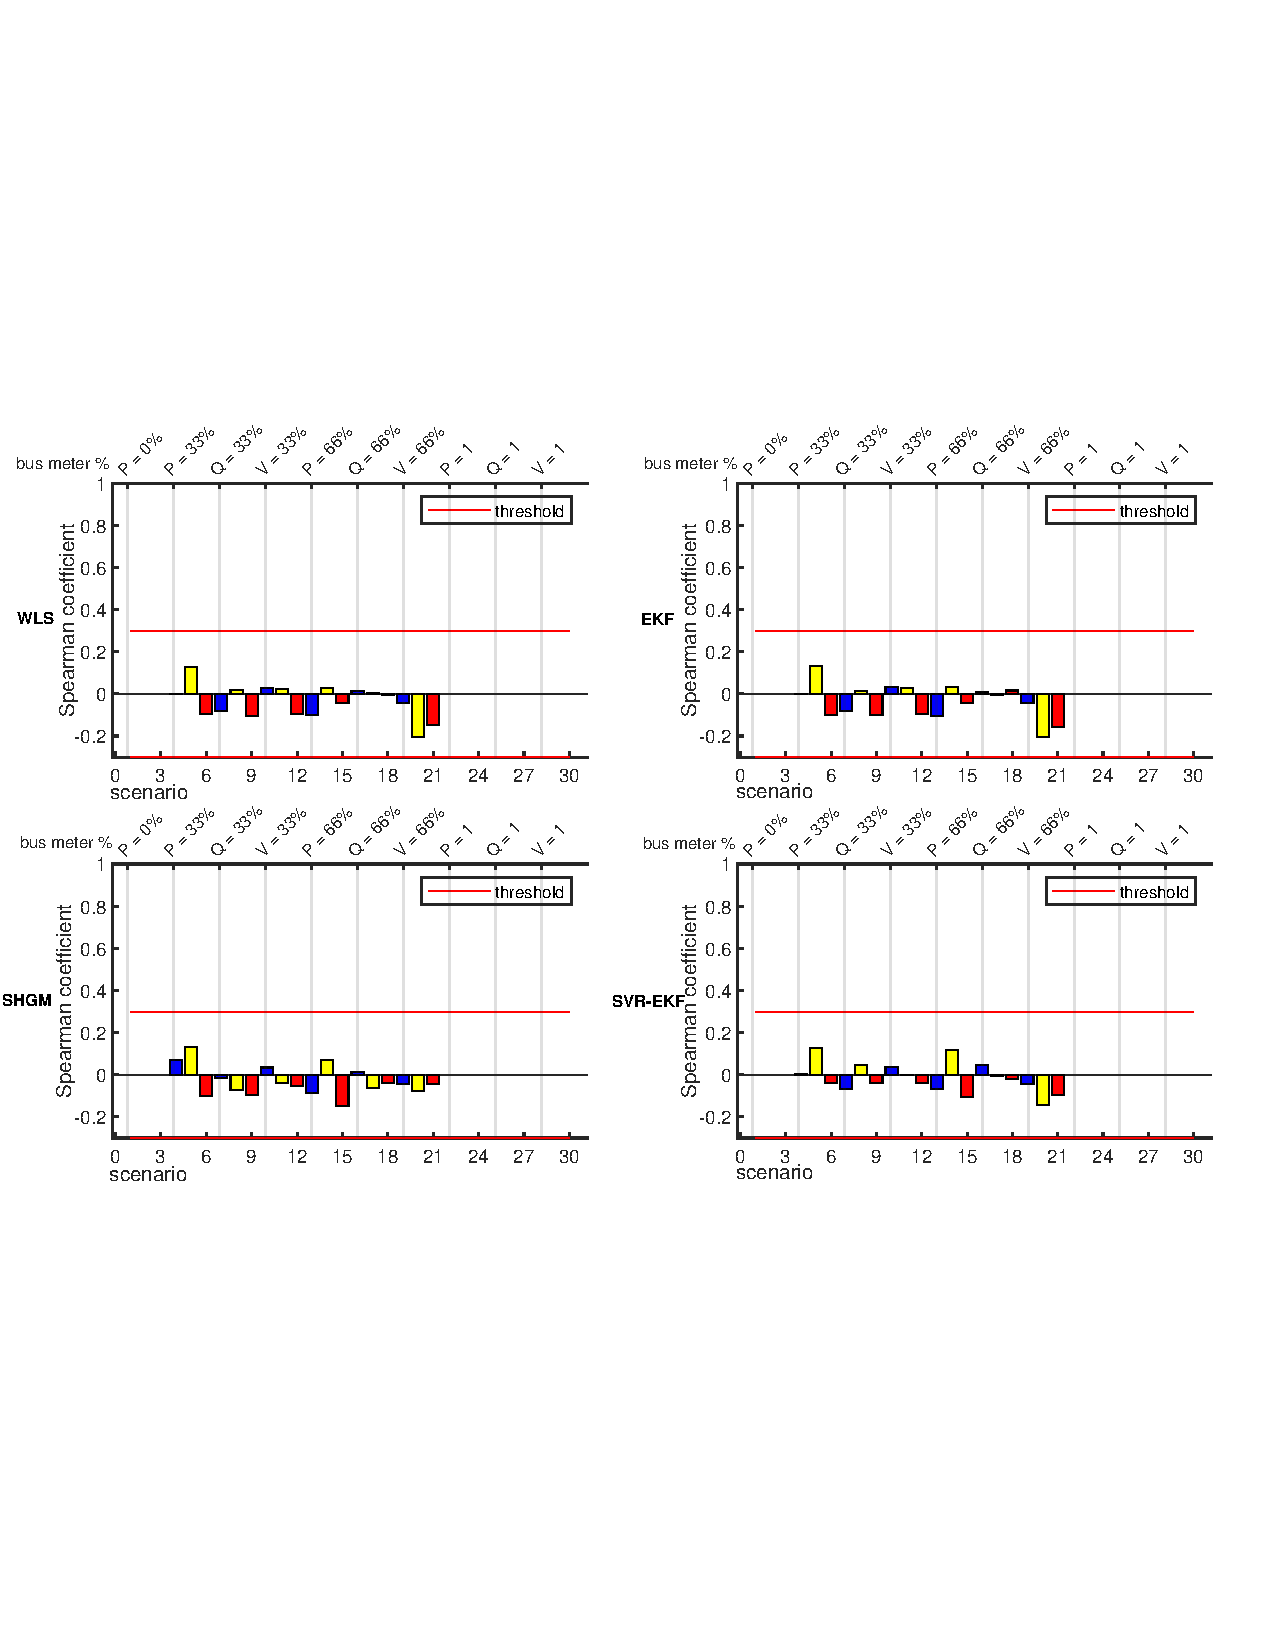
\includegraphics[ height=8cm, width=14cm]{figures/appendix/spearman_bus_meter_P.pdf}
        \caption{Spearman coefficient $p(RMSE^{P_{flow}},dist^{bus})$}
    \end{figure}
    
    \begin{figure}[!htb]
        \centering
        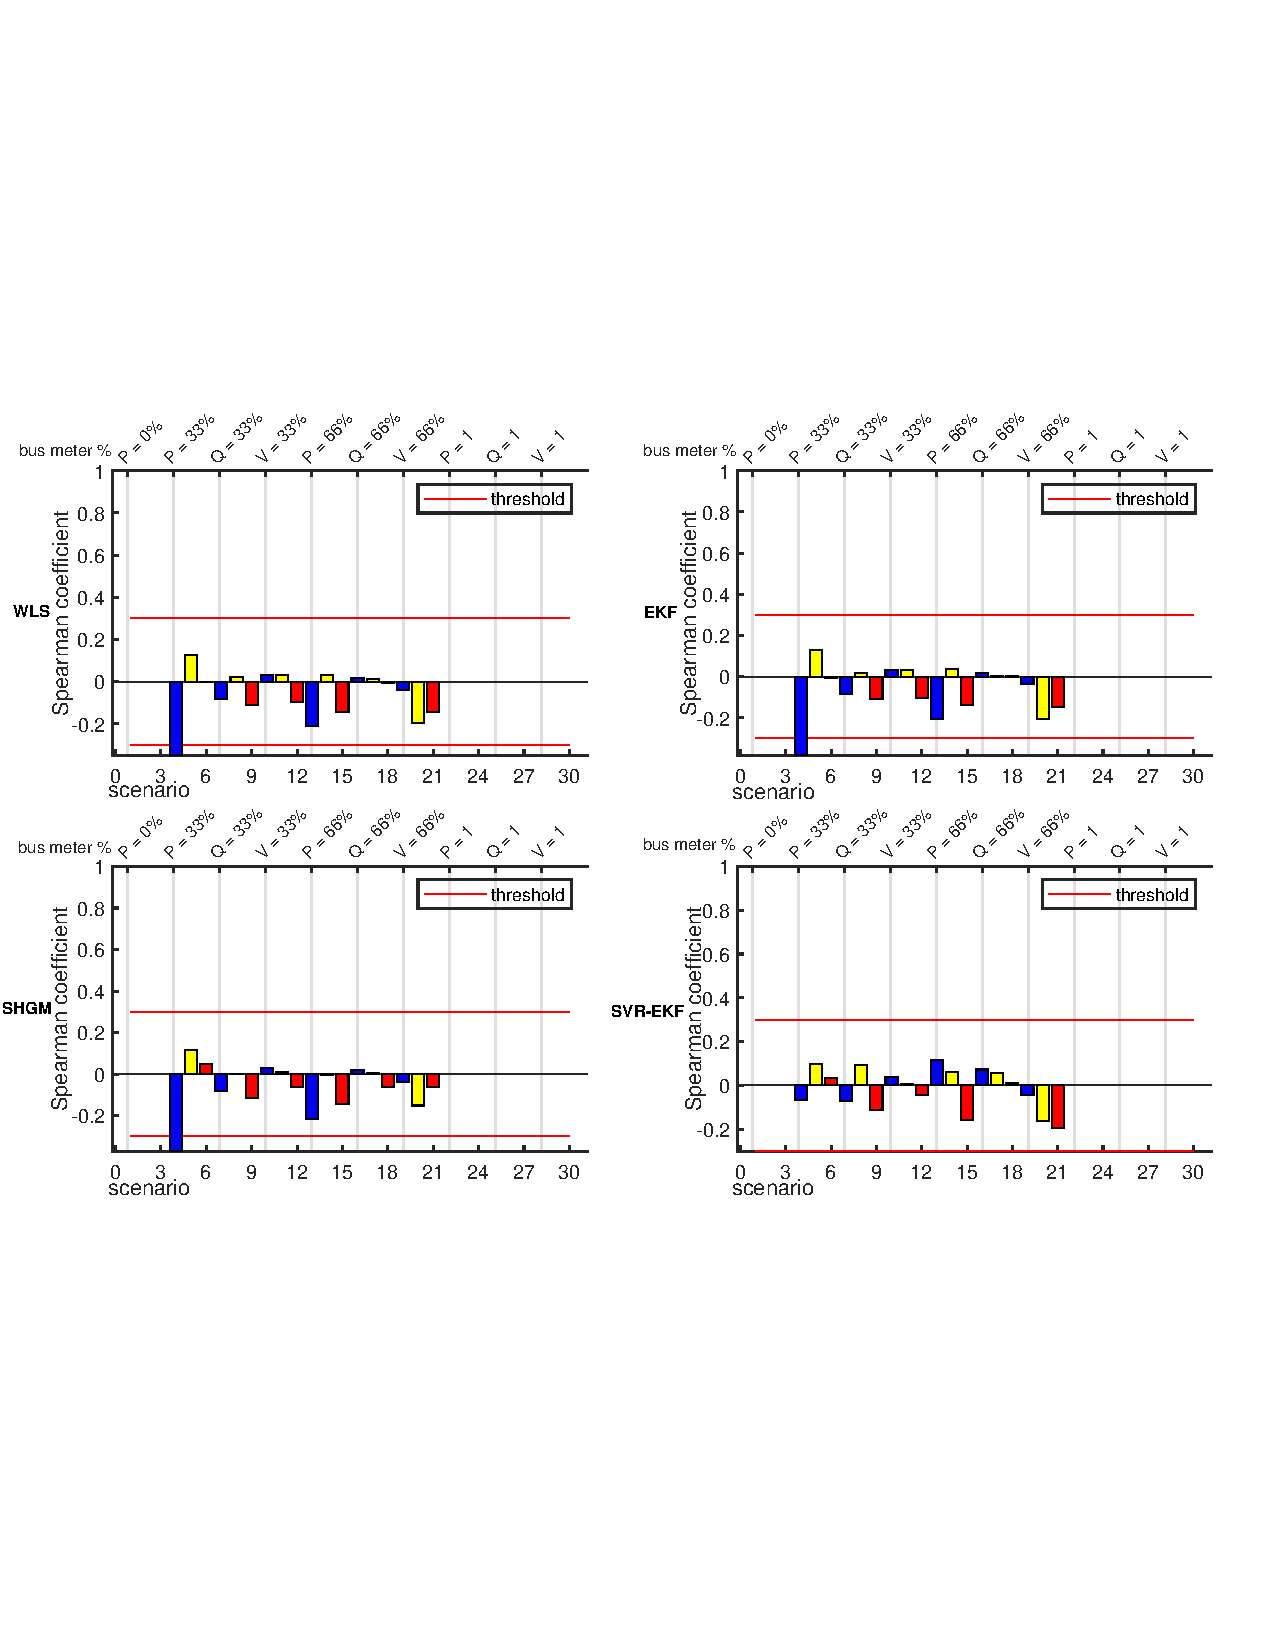
\includegraphics[ height=8cm, width=14cm]{figures/appendix/spearman_bus_meter_Q.pdf}
        \caption{Spearman coefficient $p(RMSE^{Q_{flow}},dist^{bus})$}
    \end{figure}
    
\FloatBarrier

\subsection{Branch Meters Distance to the Feeder Bus}

    \begin{figure}[!htb]
        \centering
        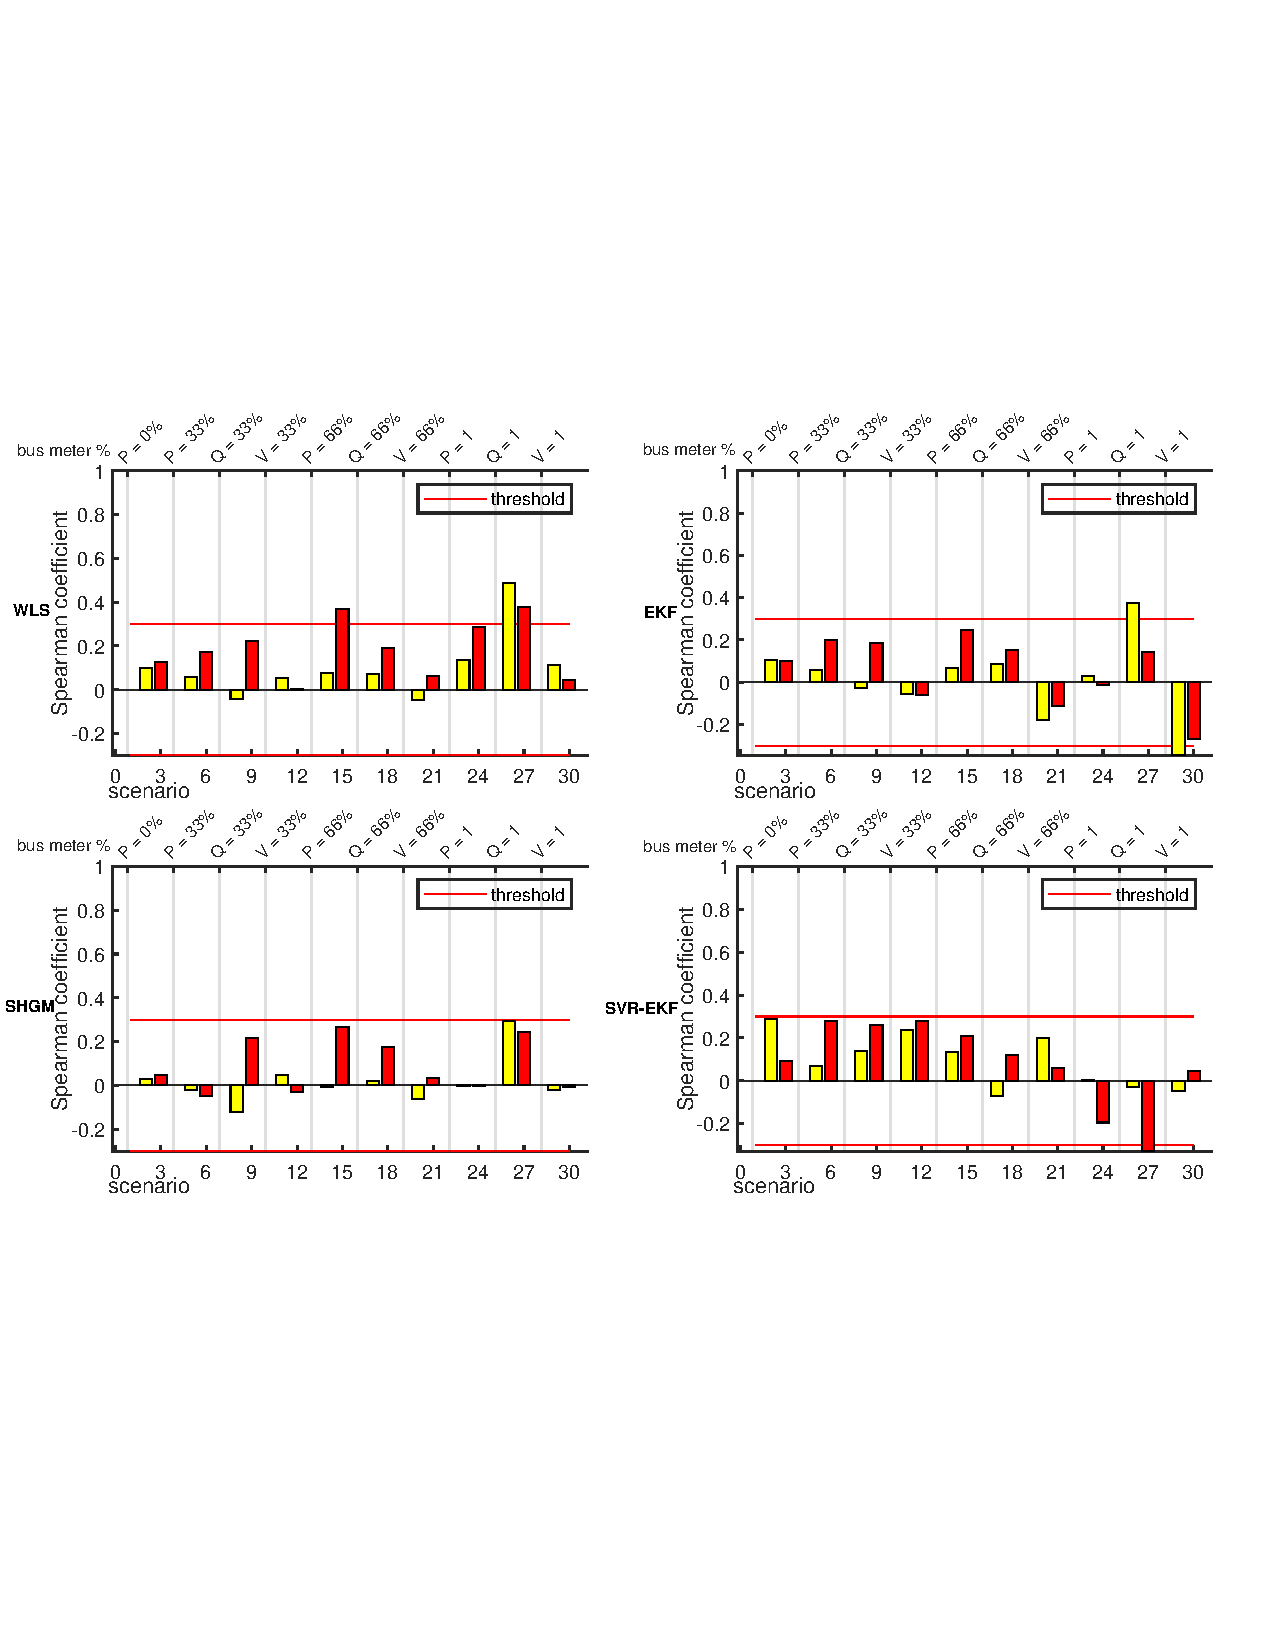
\includegraphics[ height=8cm, width=14cm]{figures/appendix/spearman_dist_branch_V.pdf}
        \caption{Spearman coefficient $p(RMSE^V,dist^{branch})$}
    \end{figure}

    \begin{figure}[!htb]
        \centering
        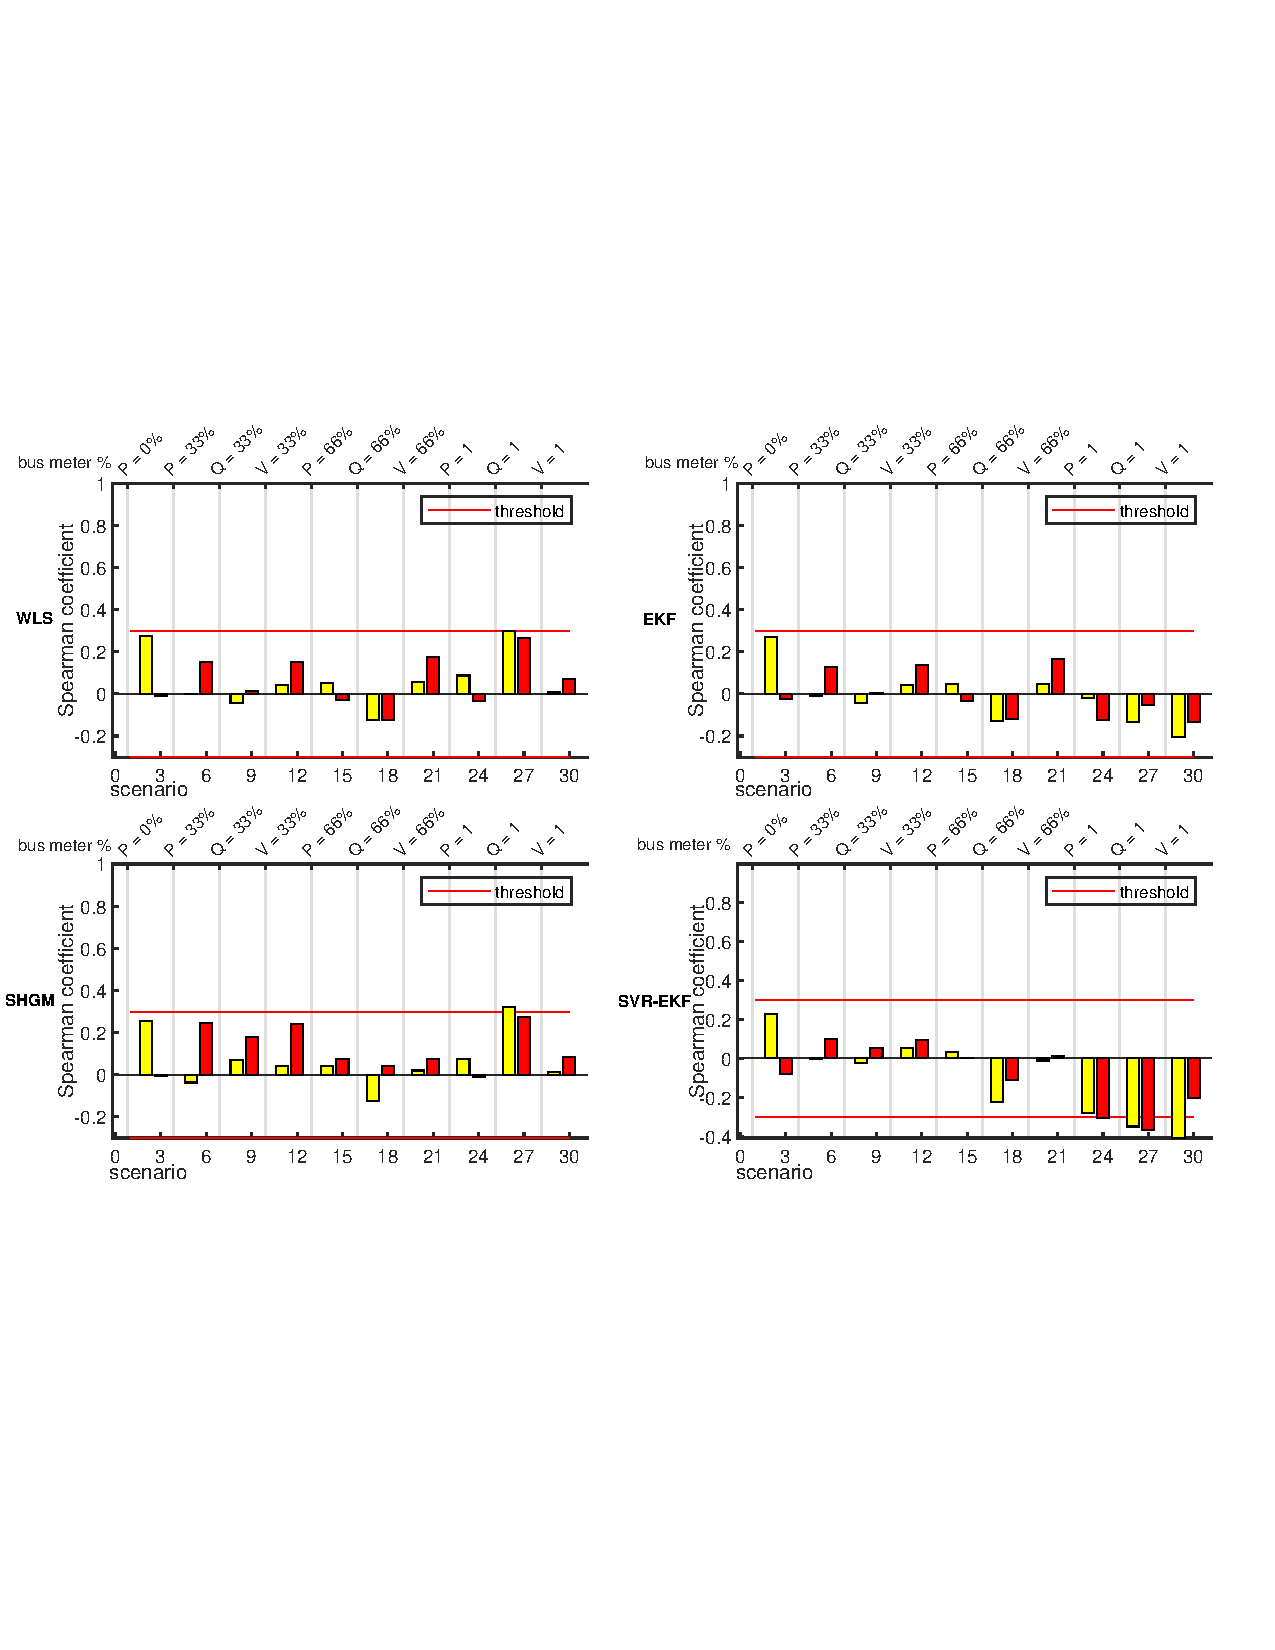
\includegraphics[ height=8cm, width=14cm]{figures/appendix/spearman_dist_branch_P.pdf}
        \caption{Spearman coefficient $p(RMSE^{P_{flow}},dist^{branch})$}
    \end{figure}
    
    \begin{figure}[!htb]
        \centering
        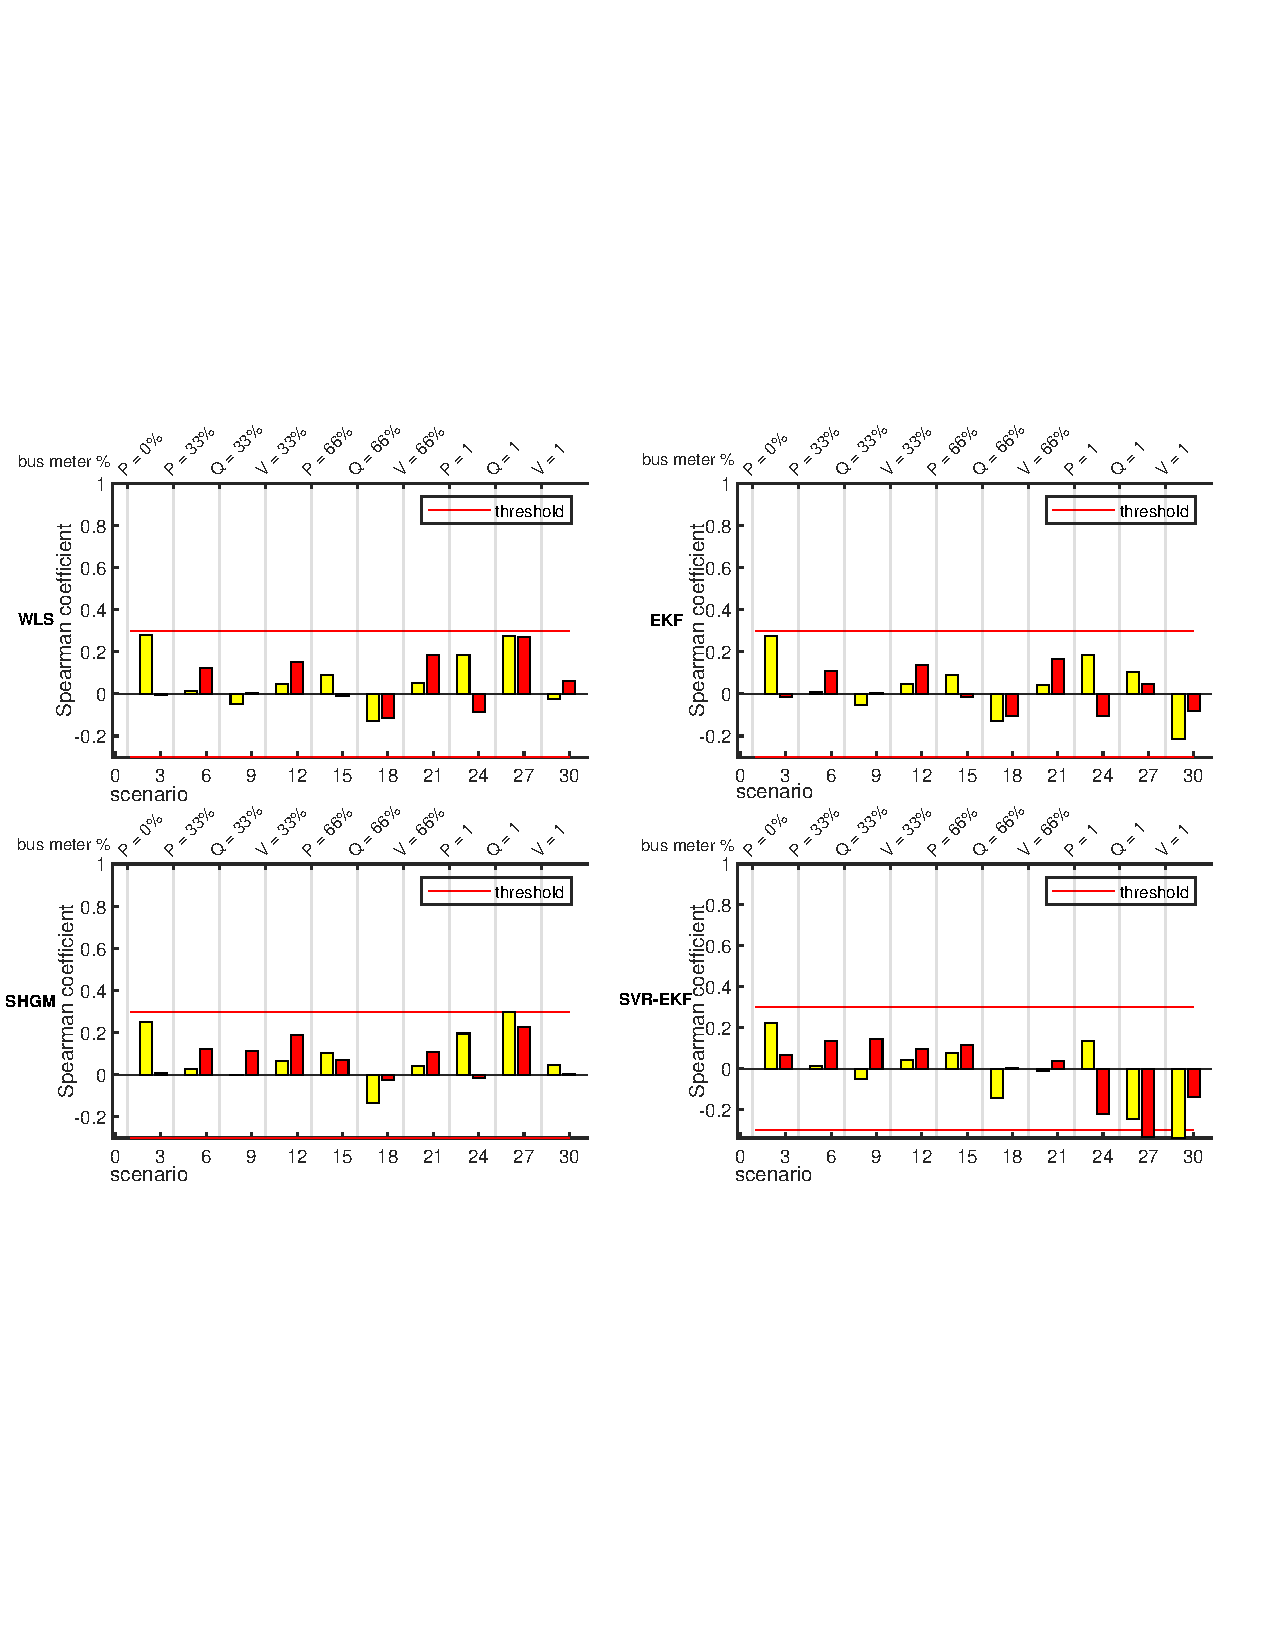
\includegraphics[ height=8cm, width=14cm]{figures/appendix/spearman_dist_branch_Q.pdf}
        \caption{Spearman coefficient $p(RMSE^{Q_{flow}},dist^{branch})$}
    \end{figure}
\FloatBarrier


\subsection{Bus Meters Distribution by BFS}

    \begin{figure}[!htb]
        \centering
        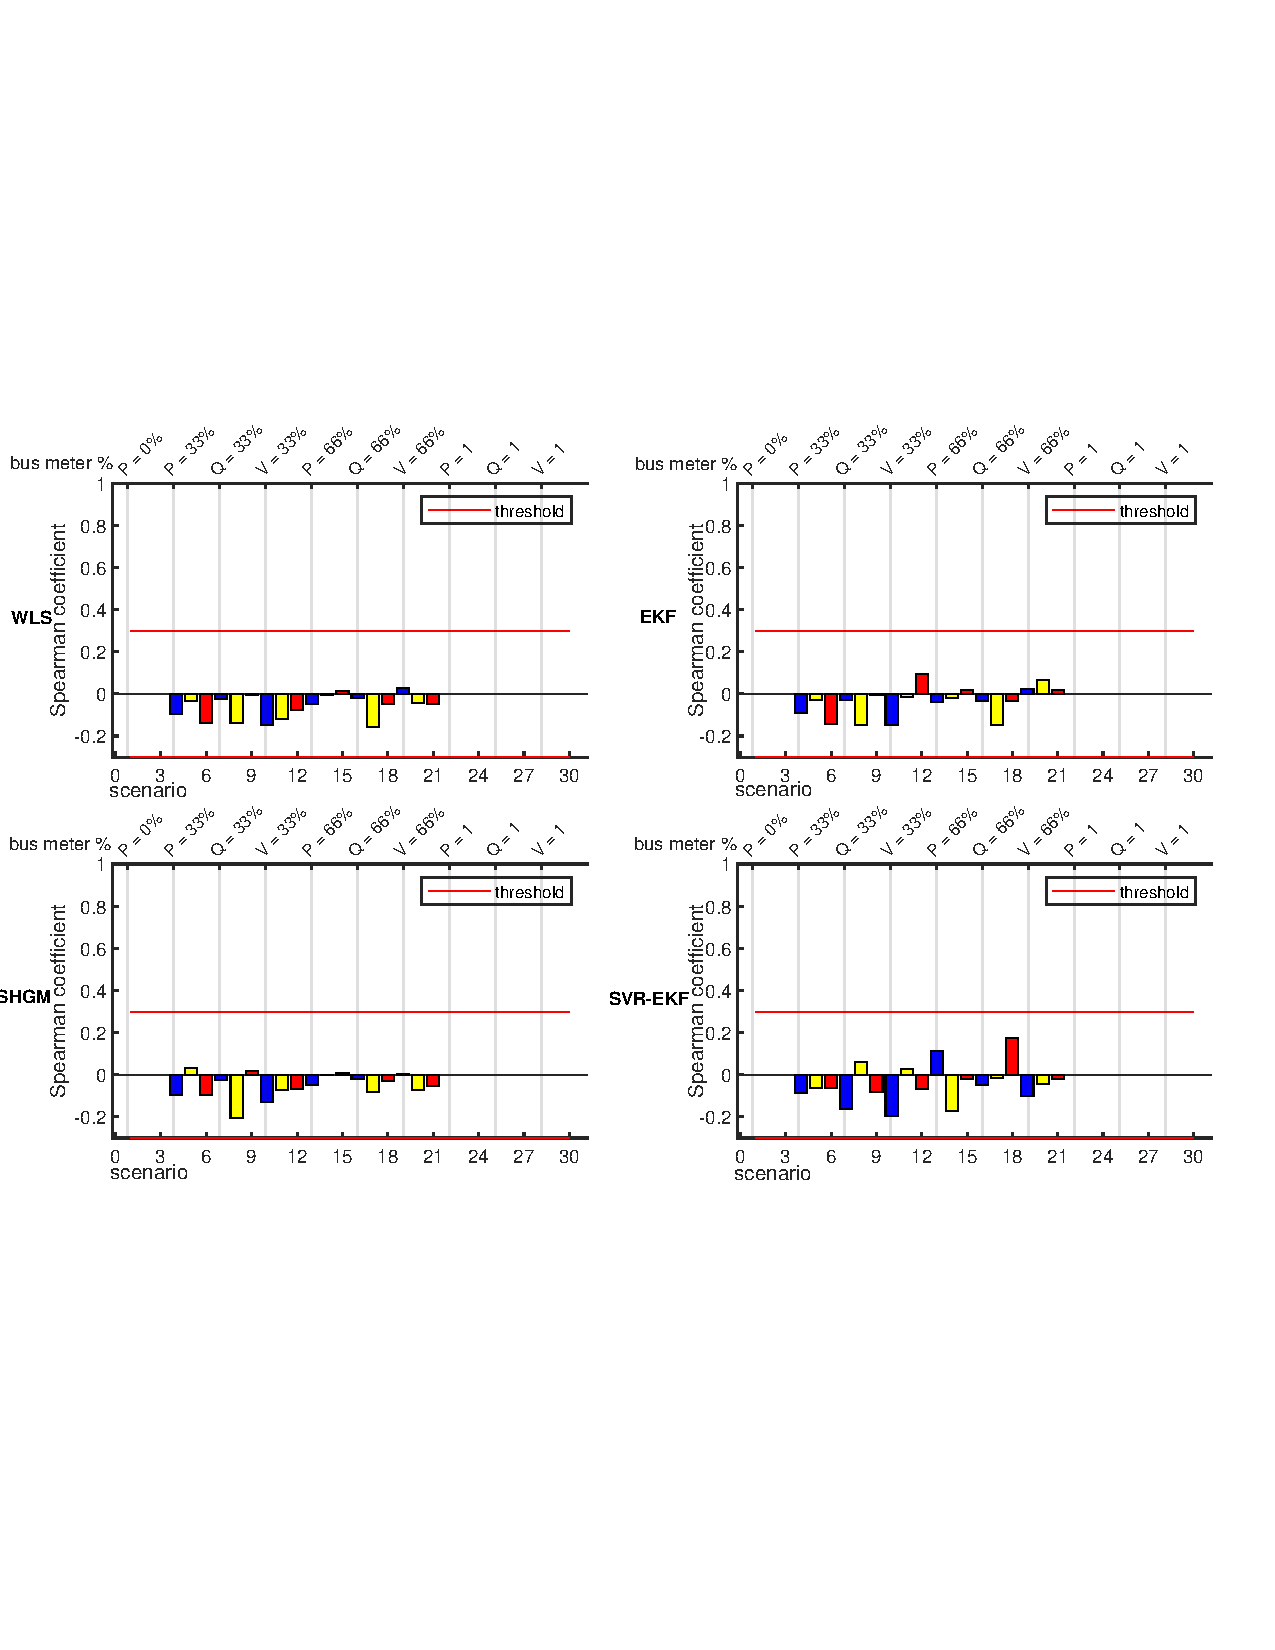
\includegraphics[ height=8cm, width=14cm]{figures/appendix/bfs_dis_bus_v.pdf}
        \caption{Spearman coefficient $p(RMSE^V,distr^{bus})$ by BFS}
        \label{fig:app_db_bus_v}
    \end{figure}
    
    \begin{figure}[!htb]
        \centering
        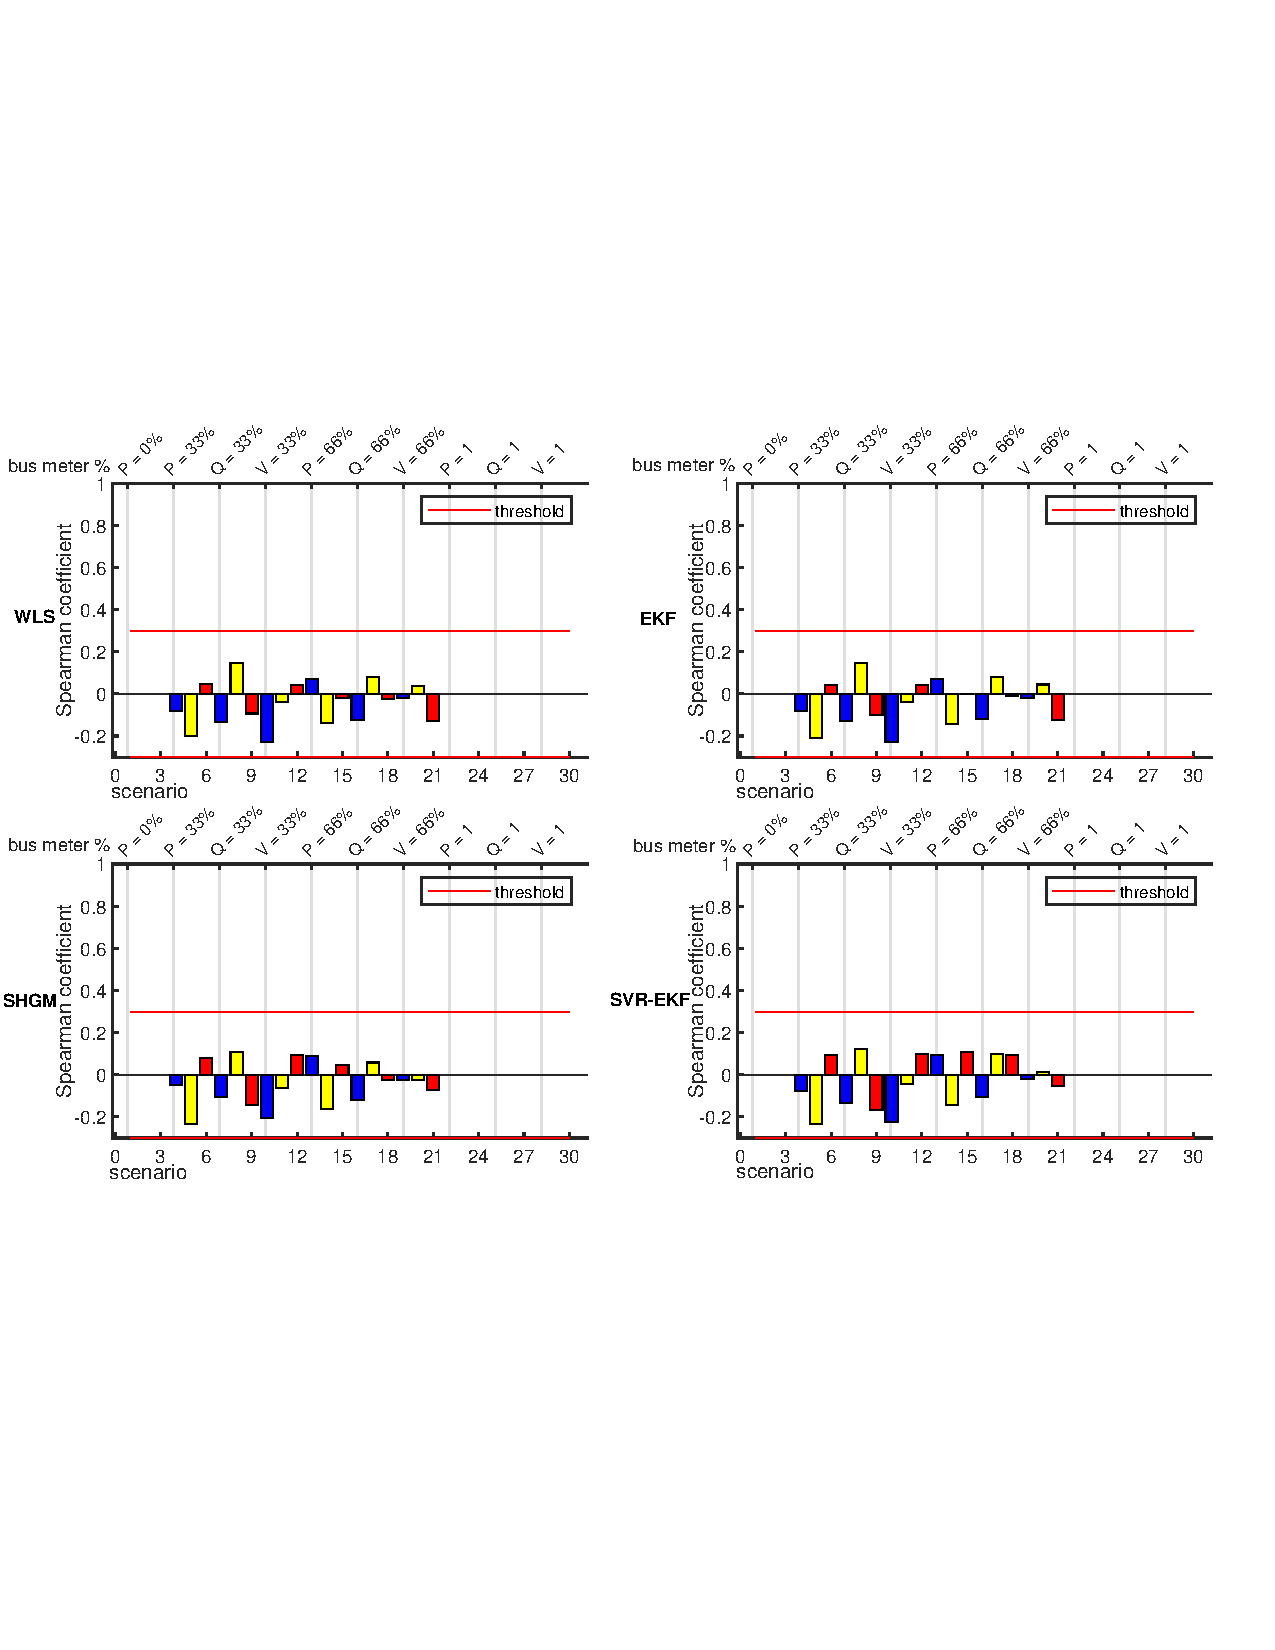
\includegraphics[ height=8cm, width=14cm]{figures/appendix/bfs_dis_bus_pflow.pdf}
        \caption{Spearman coefficient $p(RMSE^{P_{flow}},distr^{bus})$ by BFS}
        \label{fig:app_db_bus_pflow}
    \end{figure}
    
    \begin{figure}[!htb]
        \centering
        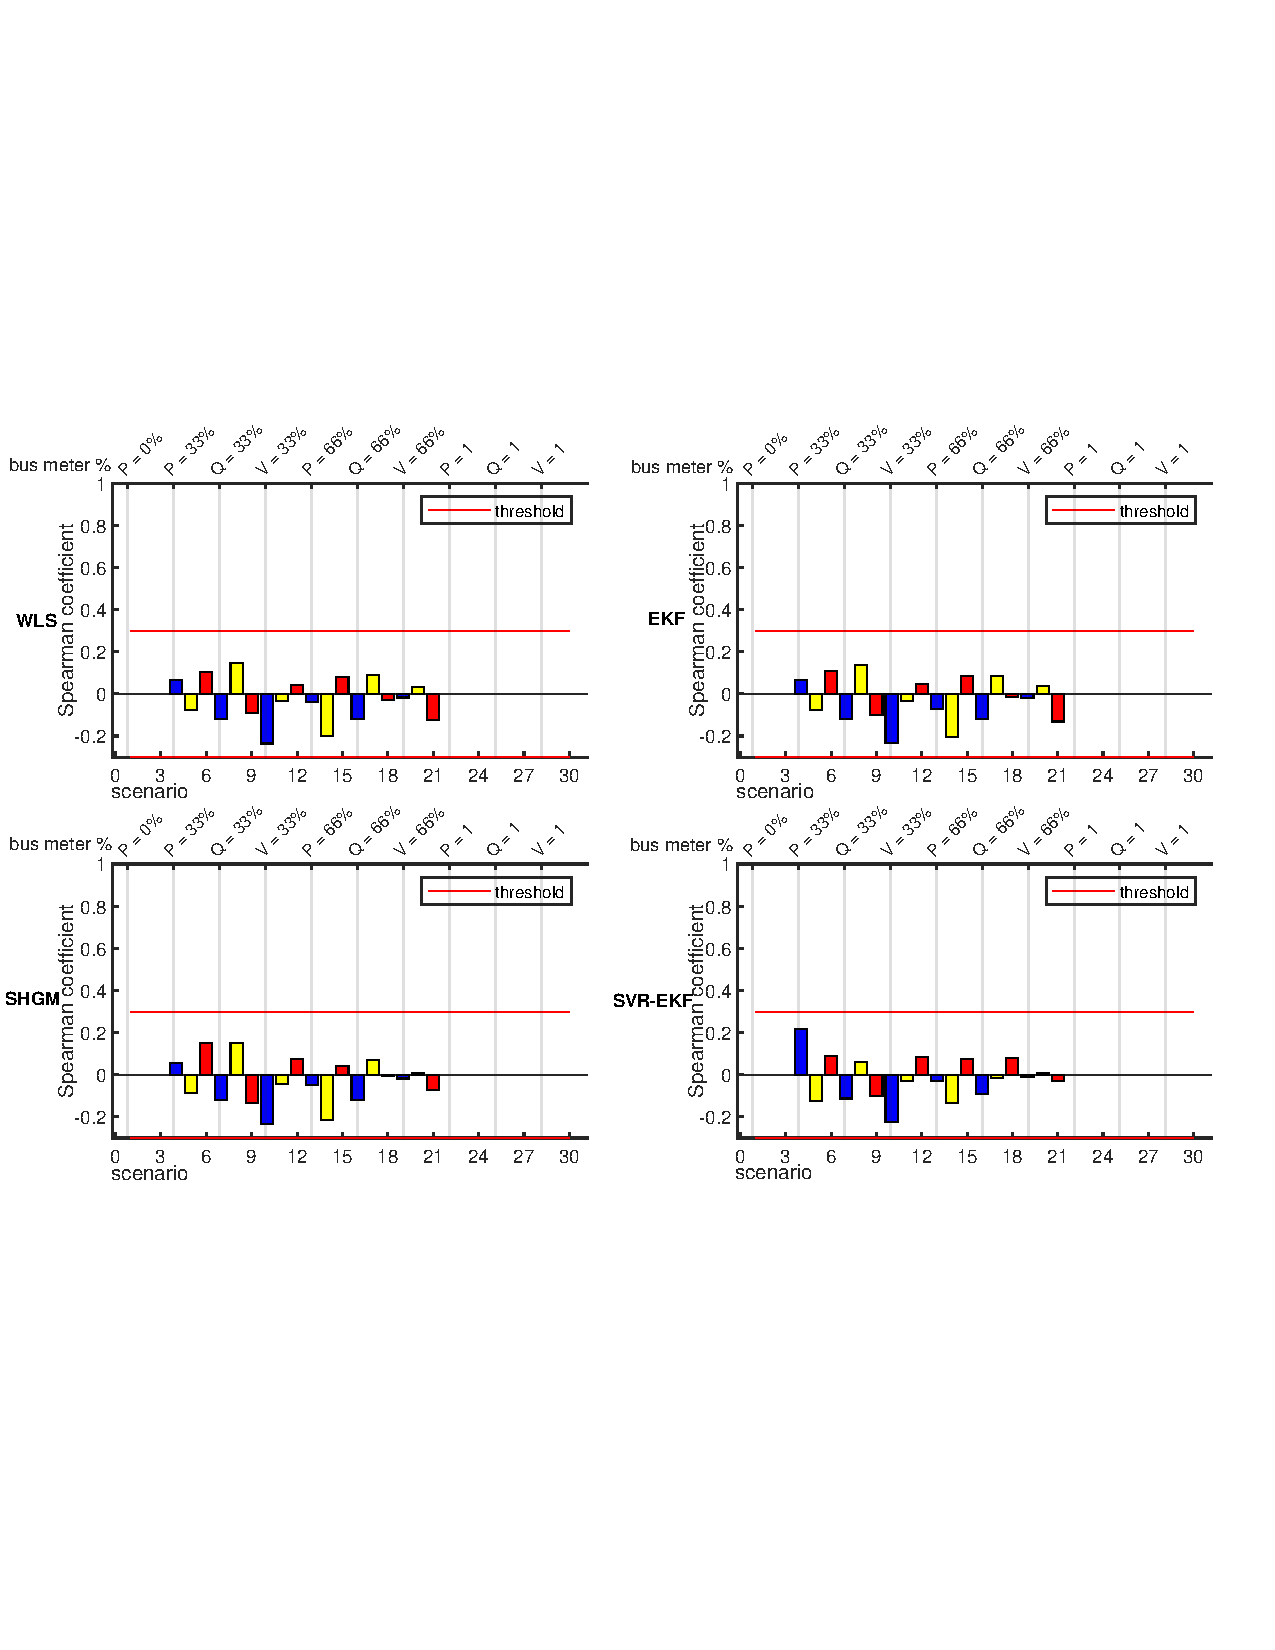
\includegraphics[ height=8cm, width=14cm]{figures/appendix/bfs_dis_bus_qflow.pdf}
        \caption{Spearman coefficient $p(RMSE^{Q_{flow}},distr^{bus})$ by BFS}
        \label{fig:app_db_bus_qflow}
    \end{figure}
\FloatBarrier

\subsection{Branch Meters Distribution by BFS}
    
    \begin{figure}[!htb]
        \centering
        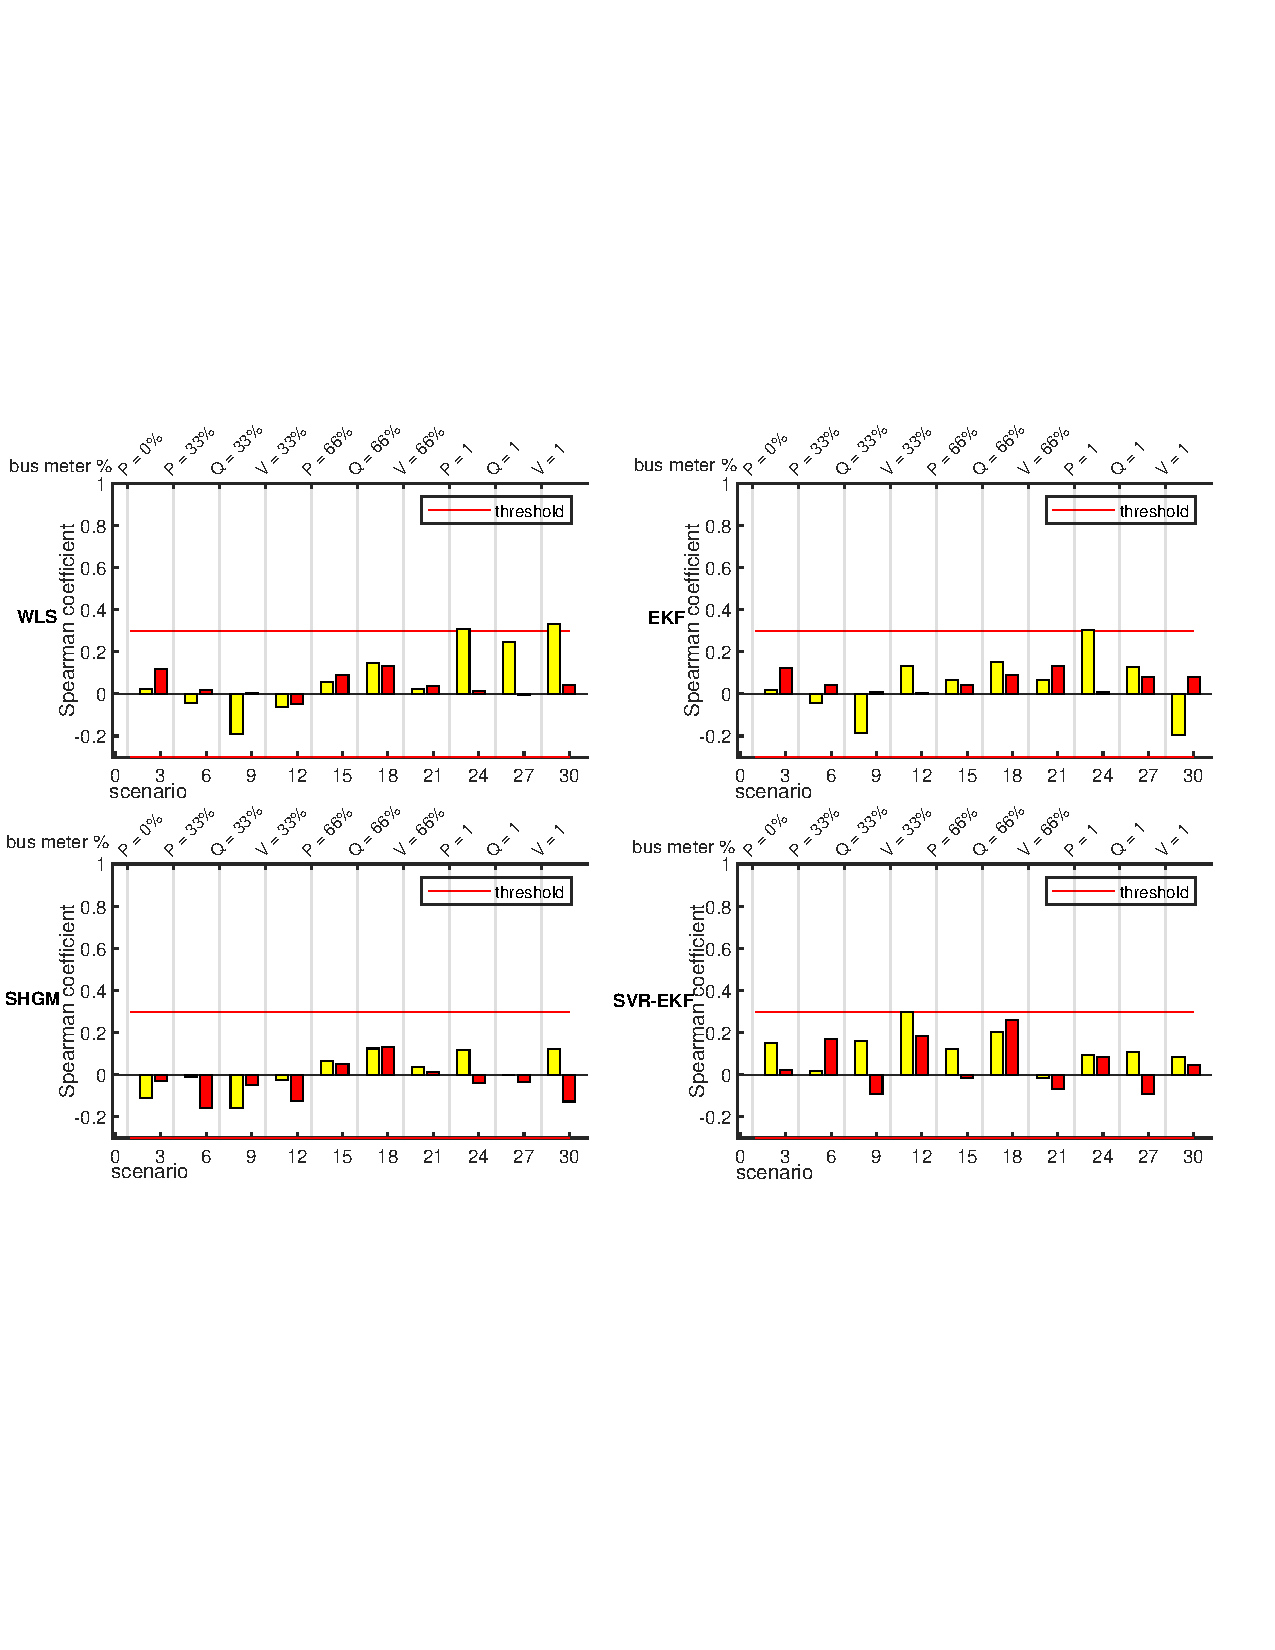
\includegraphics[ height=8cm, width=14cm]{figures/appendix/bfs_dis_branch_v.pdf}
        \caption{Spearman coefficient $p(RMSE^V,distr^{branch})$ by BFS}
        \label{fig:app_db_branch_v}
    \end{figure}
    
    \begin{figure}[!htb]
        \centering
        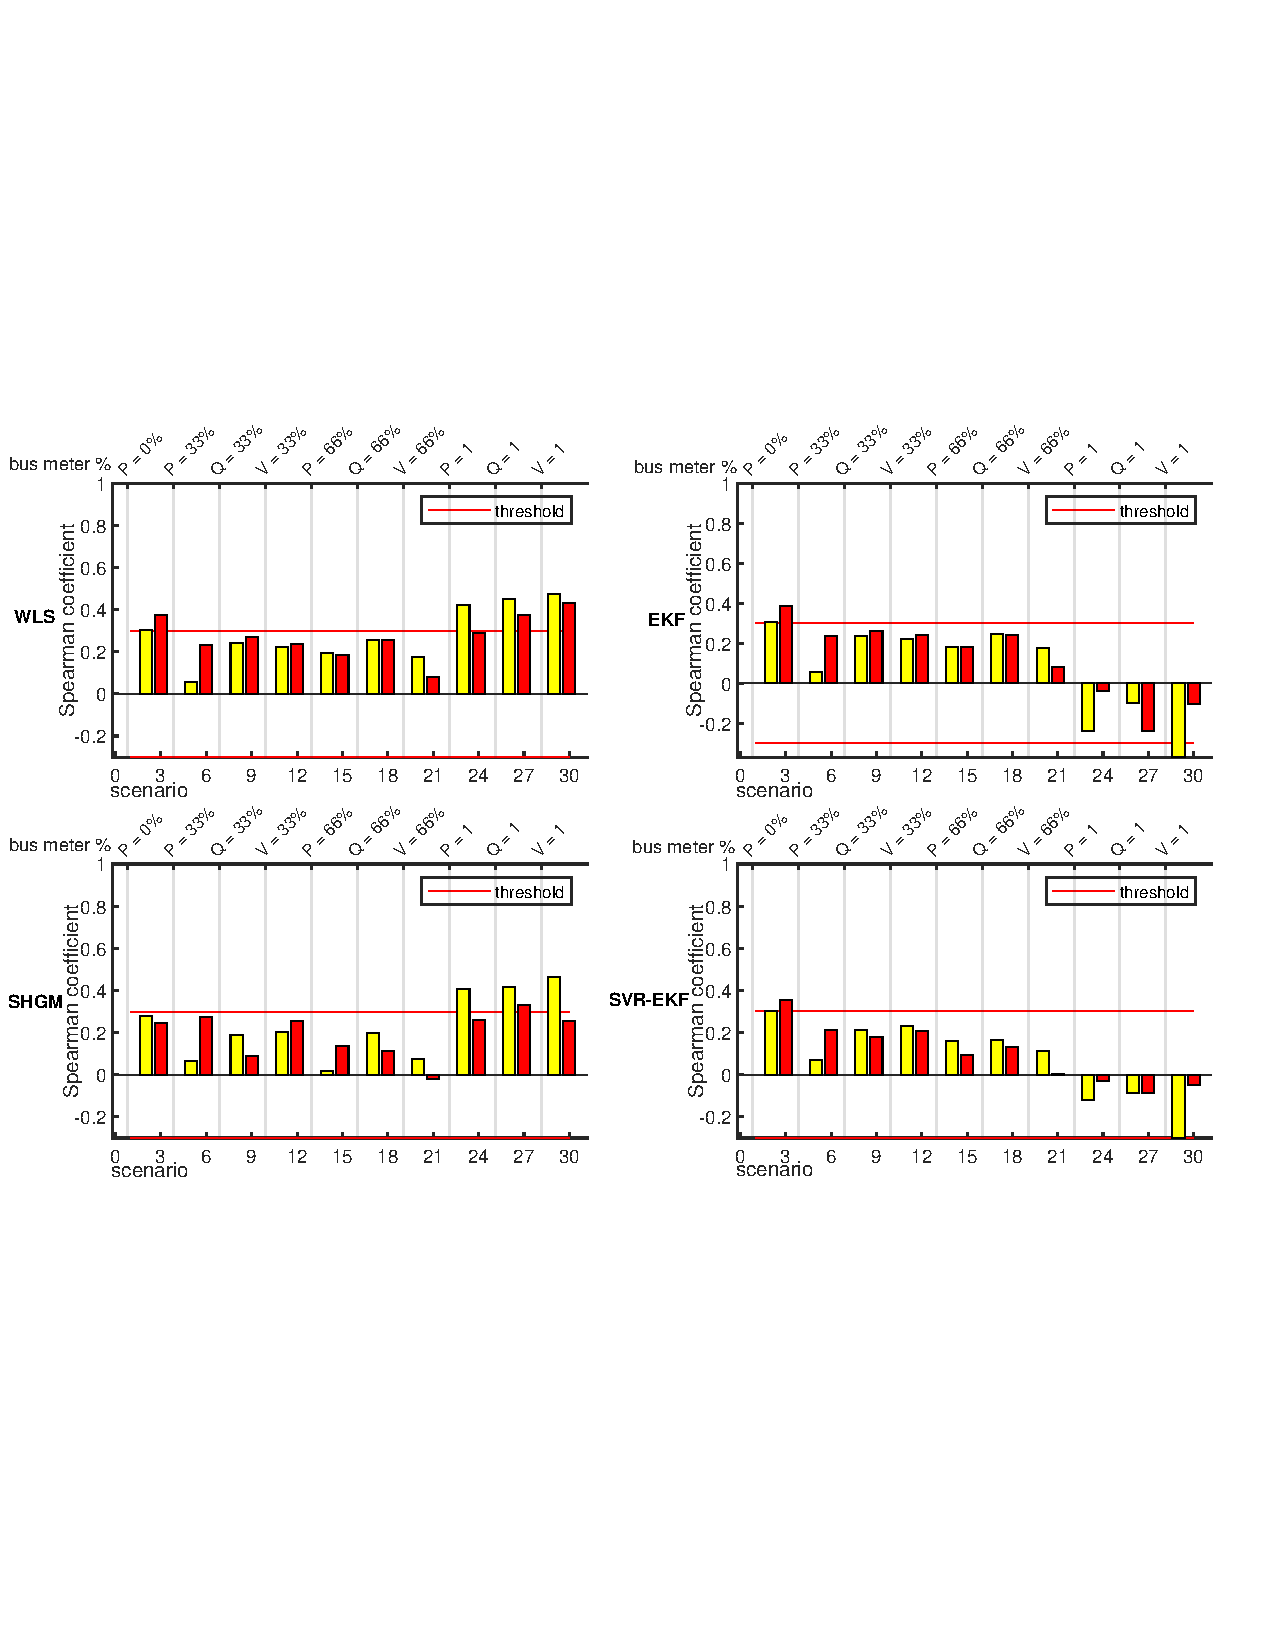
\includegraphics[ height=8cm, width=14cm]{figures/appendix/bfs_dis_branch_pflow.pdf}
        \caption{Spearman coefficient $p(RMSE^{P_{flow}},distr^{branch})$ by BFS}
        \label{fig:app_db_branch_pflow}
    \end{figure}
    
    \begin{figure}[!htb]
        \centering
        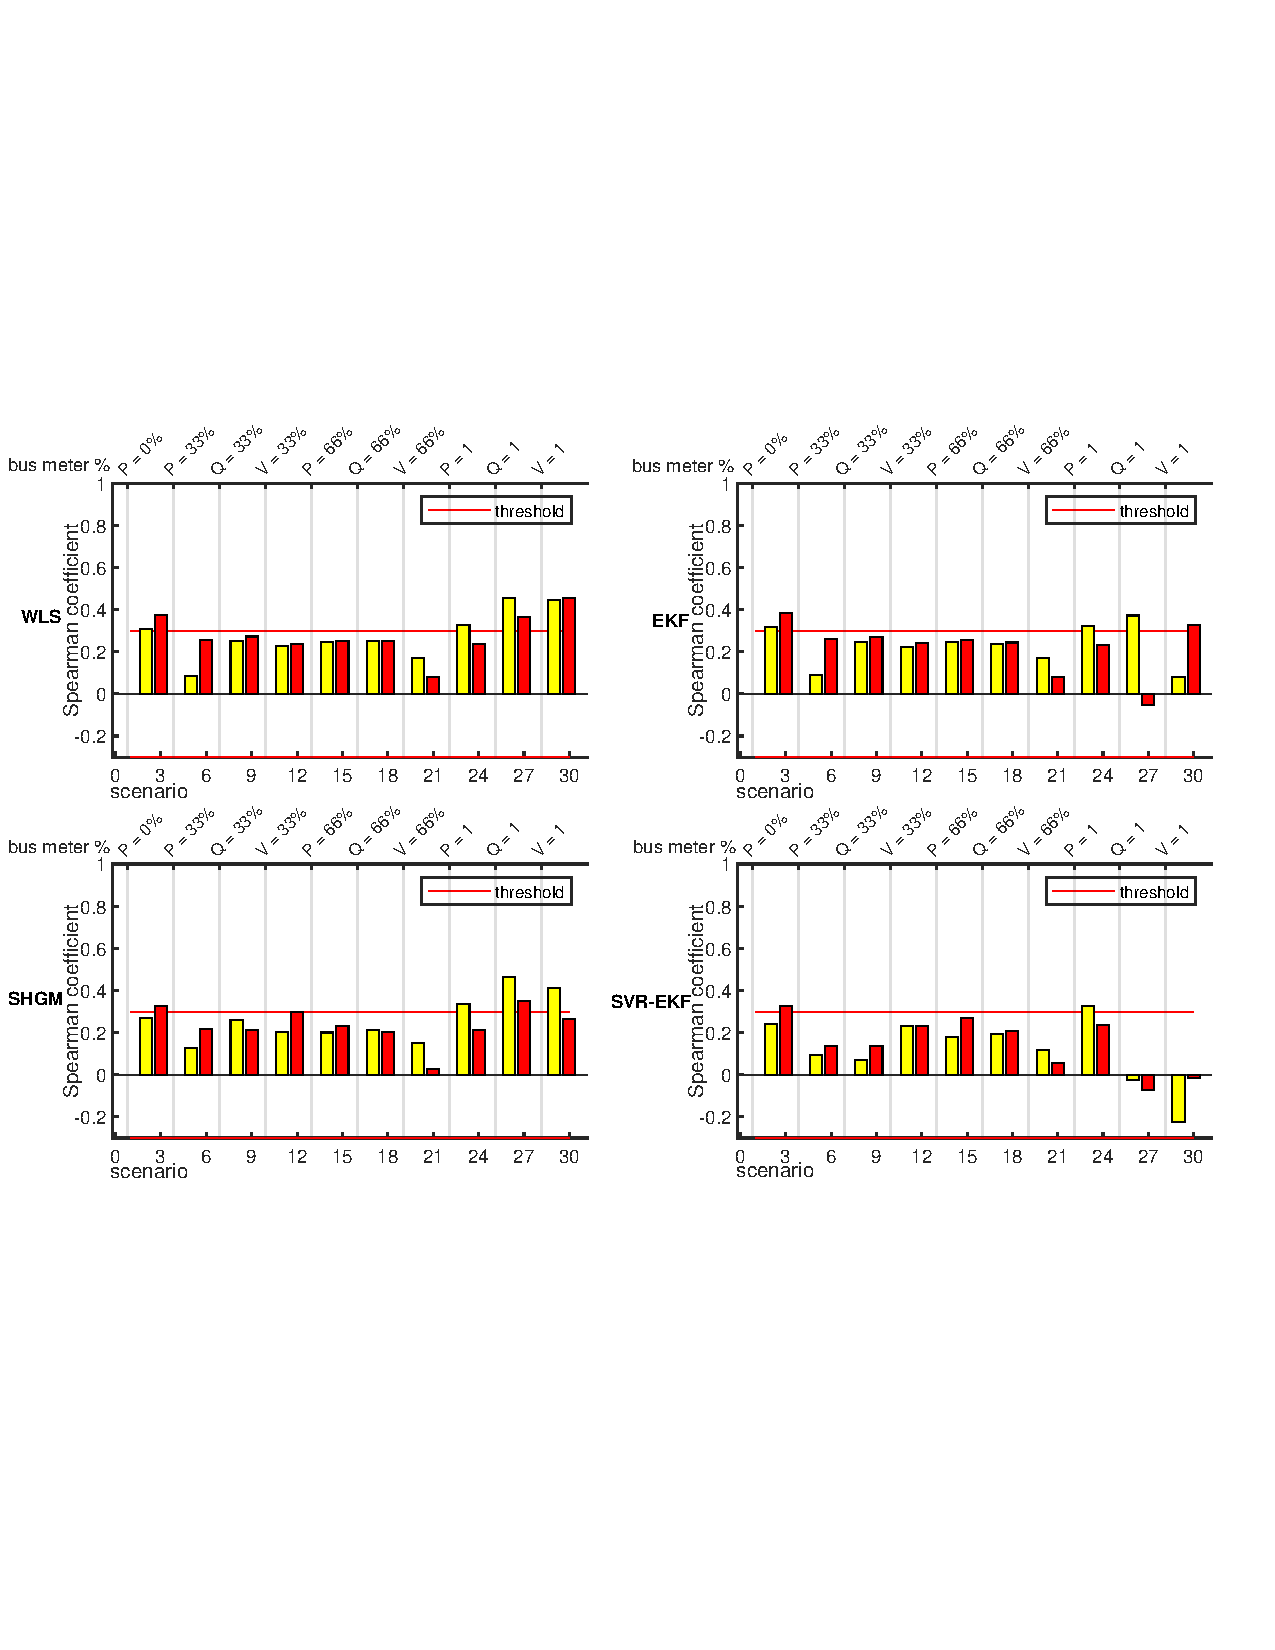
\includegraphics[ height=8cm, width=14cm]{figures/appendix/bfs_dis_branch_qflow.pdf}
        \caption{Spearman coefficient $p(RMSE^{Q_{flow}},distr^{branch})$ by BFS}
        \label{fig:app_db_branch_qflow}
    \end{figure}
\FloatBarrier    
    
\subsection{Bus Meters Distribution by Path Search}    
    
    \begin{figure}[!h]
        \centering
        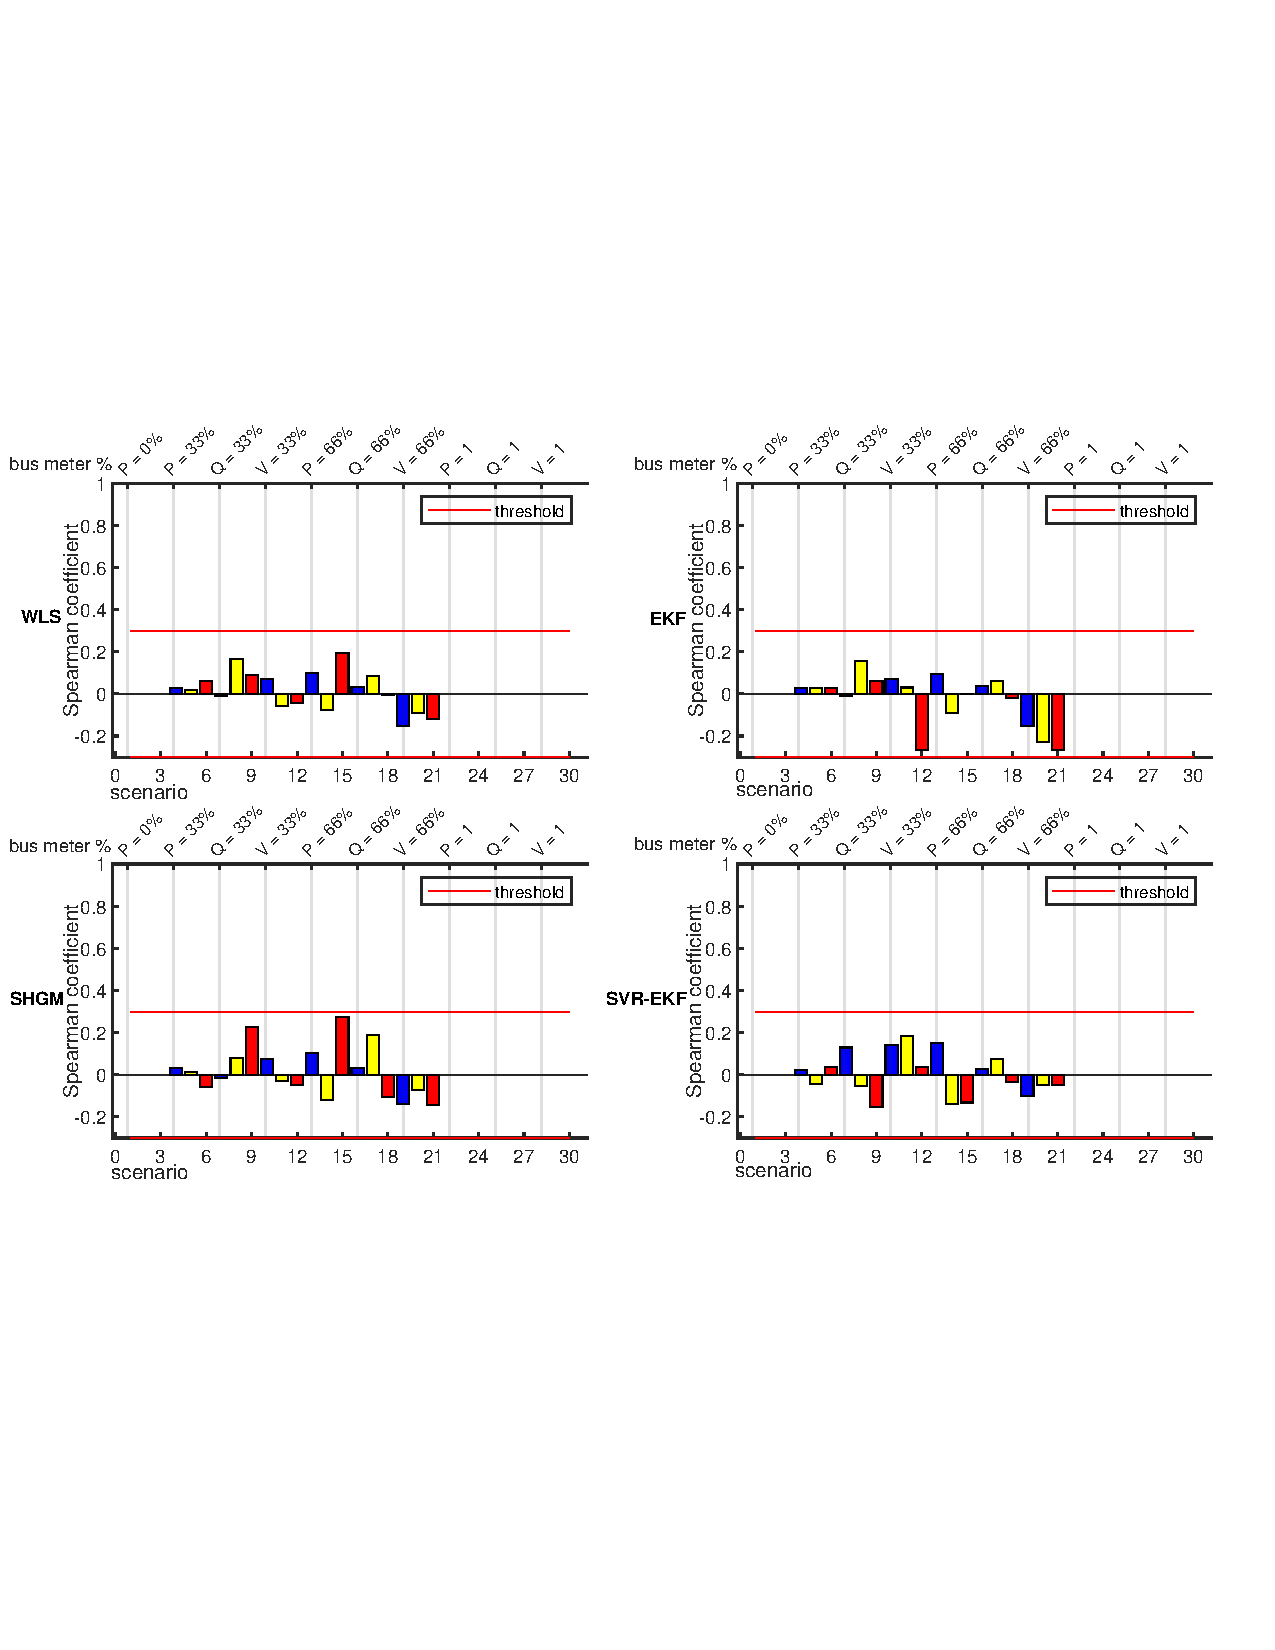
\includegraphics[ height=8cm, width=14cm]{figures/appendix/path_dis_bus_v.pdf}
        \caption{Spearman coefficient $p(RMSE^V,distr^{bus})$ by Path Search}
        \label{fig:app_db_bus_v_path}
    \end{figure}
    
    \begin{figure}[!h]
        \centering
        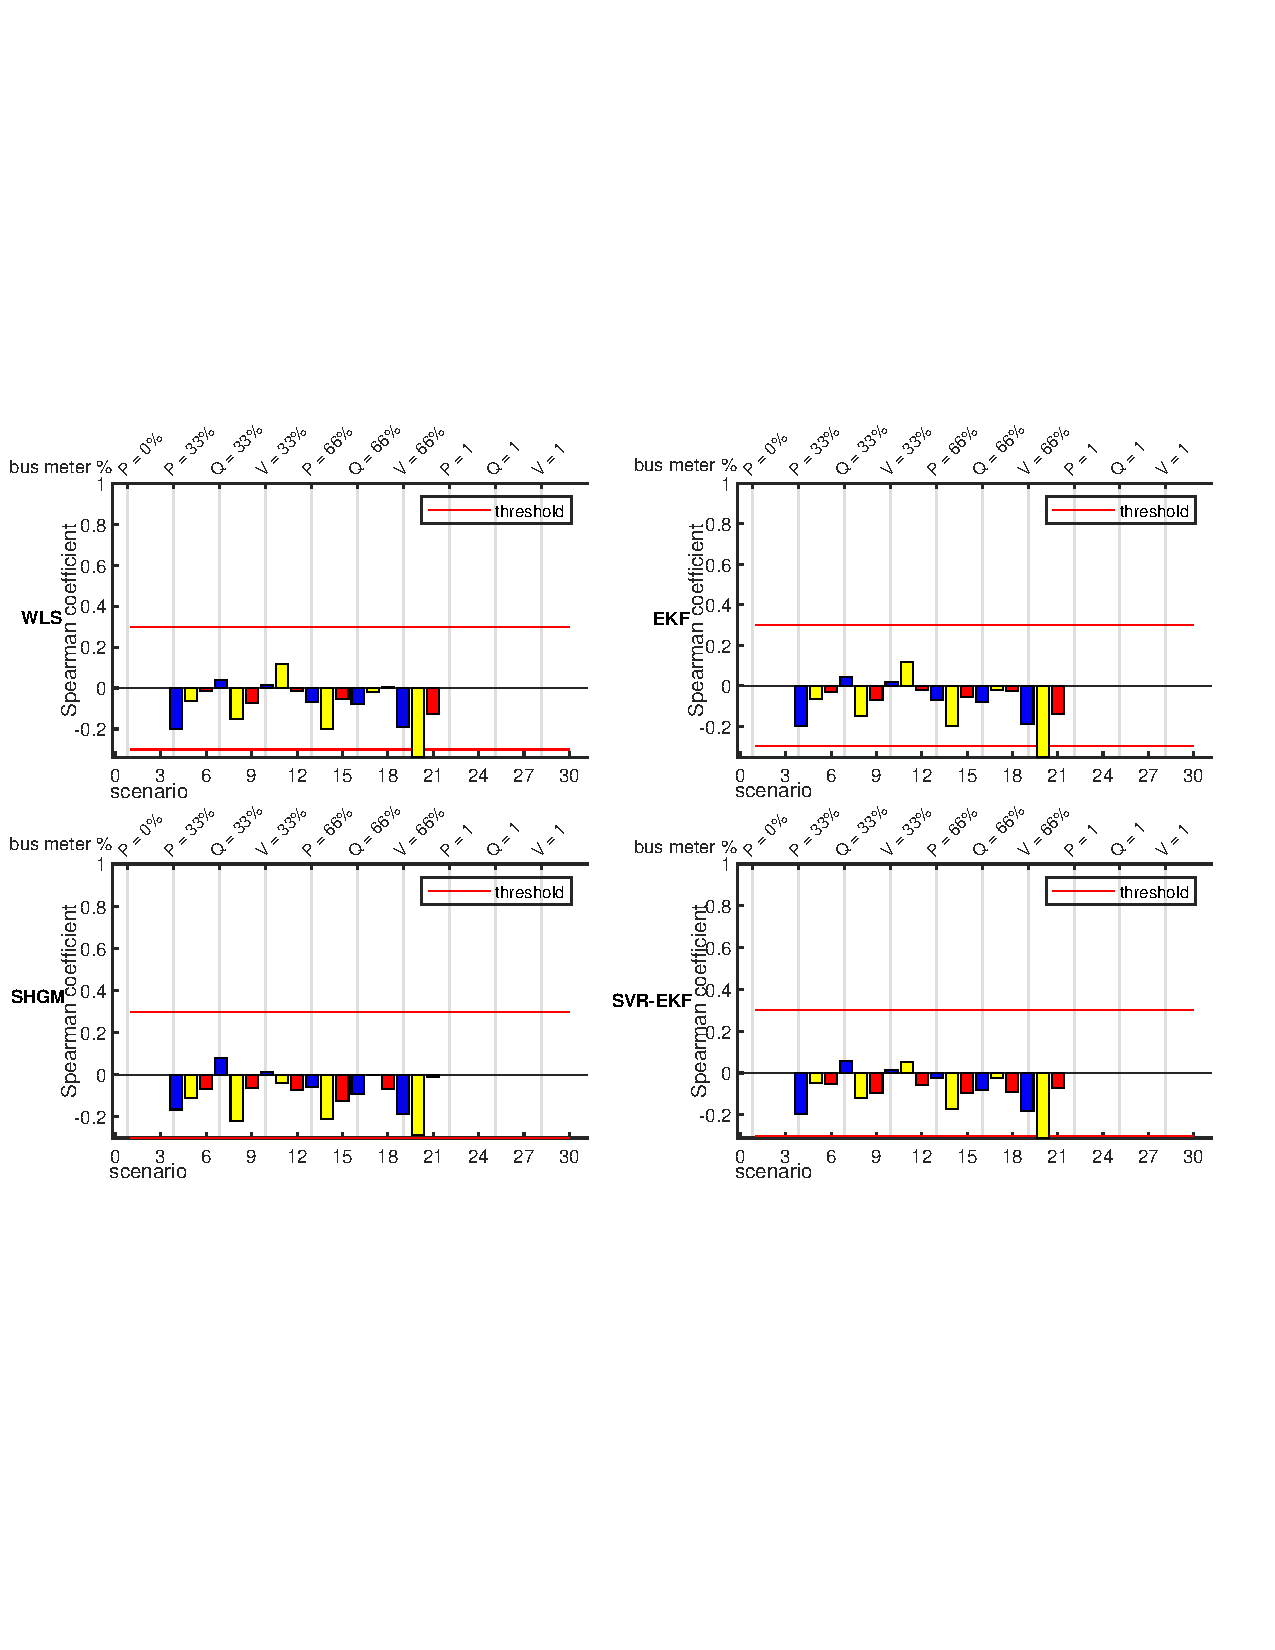
\includegraphics[ height=8cm, width=14cm]{figures/appendix/path_dis_bus_pflow.pdf}
        \caption{Spearman coefficient $p(RMSE^{P_{flow}},distr^{bus})$ by Path Search}
        \label{fig:app_db_bus_pflow_path}
    \end{figure}
    
    \begin{figure}[!h]
        \centering
        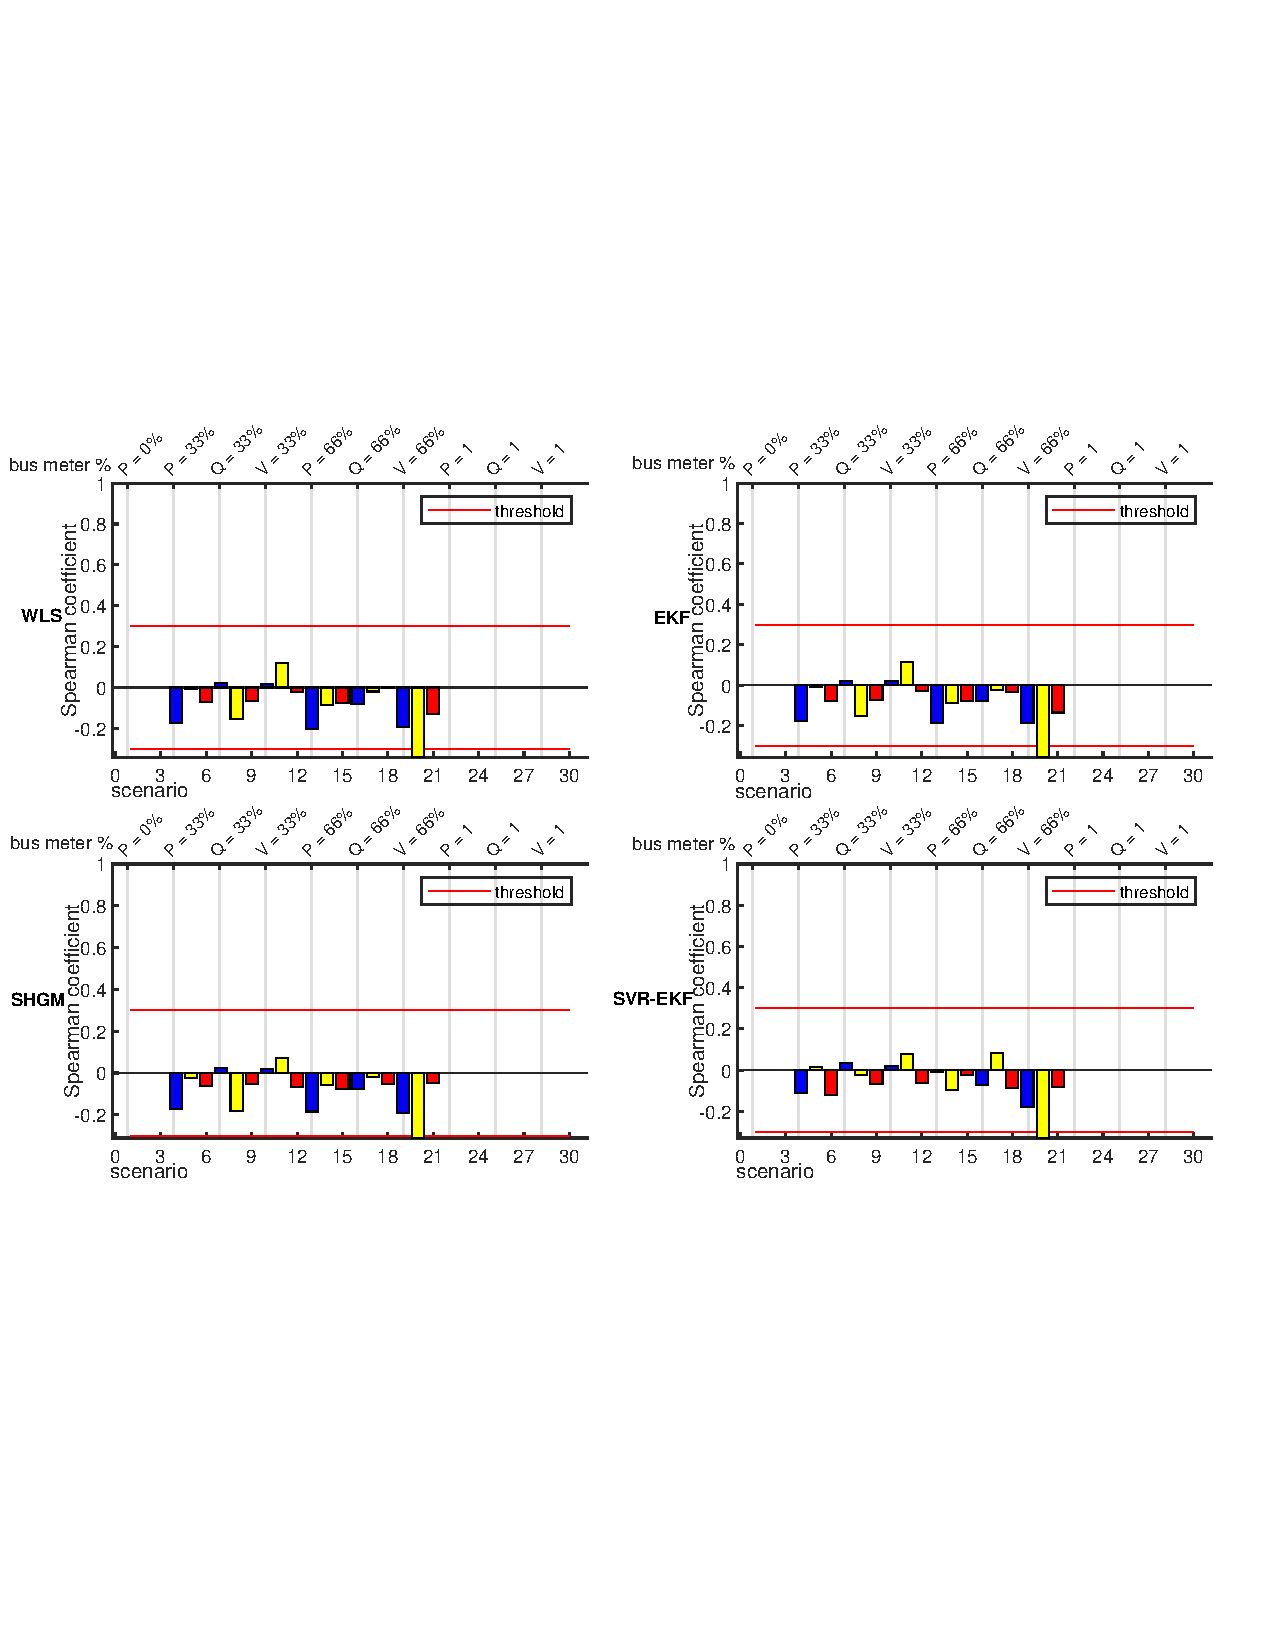
\includegraphics[ height=8cm, width=14cm]{figures/appendix/path_dis_bus_qflow.pdf}
        \caption{Spearman coefficient $p(RMSE^{Q_{flow}},distr^{bus})$ by Path Search}
        \label{fig:app_db_bus_qflow_path}
    \end{figure}
\FloatBarrier    
    
\subsection{Branch Meters Distribution by Path Search} 
    \begin{figure}[!h]
        \centering
        \includegraphics[ height=8cm, width=14cm]{figures/appendix/path_dis_branch_v.pdf}
        \caption{Spearman coefficient $p(RMSE^V,distr^{branch})$ by Path Search}
        \label{fig:app_db_branch_v_path}
    \end{figure}
    
    \begin{figure}[!h]
        \centering
        \includegraphics[ height=8cm, width=14cm]{figures/appendix/path_dis_branch_pflow.pdf}
        \caption{Spearman coefficient $p(RMSE^{P_{flow}},distr^{branch})$ by Path Search}
        \label{fig:app_db_branch_pflow_path}
    \end{figure}
    
    \begin{figure}[!h]
        \centering
        \includegraphics[ height=8cm, width=14cm]{figures/appendix/path_dis_branch_qflow.pdf}
        \caption{Spearman coefficient $p(RMSE^{Q_{flow}},distr^{branch})$ by Path Search}
        \label{fig:app_db_branch_qflow_path}
    \end{figure}
    
\section{Pearson Coefficient}

    \begin{figure}[!h]
        \centering
        \includegraphics[ height=8cm, width=14cm]{figures/appendix/bus_pflow.pdf}
        \caption{Pearson's coefficient $r(RMSE^{P_{flow}},E^{psu})$ for each scenario}
        \label{fig:app_bus_pflow}
    \end{figure}
    
    \begin{figure}[!h]
        \centering
        \includegraphics[ height=8cm, width=14cm]{figures/appendix/bus_pflow.pdf}
        \caption{Pearson's coefficient $r(RMSE^{P_{flow}},E^{psu})$ for each scenario}
        \label{fig:app_bus_pflow}
    \end{figure}

    \begin{figure}[!h]
        \centering
        \includegraphics[ height=8cm, width=14cm]{figures/appendix/bus_qflow.pdf}
        \caption{Pearson's coefficient $r(RMSE^{Q_{flow}},E^{psu})$ for each scenario}
        \label{fig:app_bus_qflow}
    \end{figure}    

\end{appendices}

\newpage

\section{Algorithm}

\subsection{Breath-First Search (BFS)}

\begin{algorithm}[H]
\KwData{G=(V,E)}
\KwResult{hier(V)}
\Initialize{\textbf{Initialize:} $hier(v_1)=1$, $hier(v_i)=\infty$, $i=2,\cdots,n$, $L={1}$, $k=2$\;}

\While{L \neq \emptyset}{
    $L_{new} =\emptyset$\;
    
    \For{$s \in N(L):=$ \{$v \in V \mid \exists u \in L \, with 
    , \{v,u\} \in E \}$}{
        \eIf{$hier(s) \neq \infty$}{
        $do \, nothing$\;
        }{
        $hier(s)=k$\;
        
        $L_{new} = L_{new} \, \cup \, {s}$ \;
        }
        $k=k+1$\;
        
        $L=L_{new}$\;
    }  
}
\caption{Bus hierarchy by BFS}
\label{alg:Bus hier by BFS}
\end{algorithm}

\subsection{Path Search}

\begin{algorithm}[H]
\KwData{G=(V,E), V^{ext}, hier(V) }
\KwResult{Path= \{p_1,\cdots,p_{np} \}}
\Initialize{\textbf{Initialize:} $hier(v_1)=1$, $hier(v_i)=\infty$, $i=2,\cdots,n$, $L={1}$, $k=2$\;}


    \For{$s \in V^{ext}$}{
        $v_s=$ \{$v_s \in V \mid hier(v_s)=hier(s)-1  \And \{v_s, s\} \in E \}$ \;
        $v_l=v_s$\;
        \While{$v_l \neq \emptyset$}{
        $p_s^v=p_s^v \, \cup \, v_s$\;
        $p_s^e=p_s^e \, \cup \, e_s:=$ \{$e_s \in E \mid e_s=\{v_s,s\}\}$ \;
        $v_l=$ \{$v_l \in V \mid hier(v_l)=hier(v_s)-1 \in V \And \{v_s, v_l\} \in E \}$ \;
        $v_s=v_l$\;
        }{
        $p_s=\{p_s^v, \, p_s^e \}$\;
        $Path=Path \, \cup \, p_s$\;
        }
    }  

\caption{Searching Paths}
\label{alg:search path}
\end{algorithm}

\subsection{Search Closest metered bus by BFS}

\begin{algorithm}[H]
\KwData{G=(V,E), M_{i,j}^{bus}}
\KwResult{dist_{i,j}^{close}{(v_{red})}}
\Initialize{\textbf{Initialize:} $L=\{v_{red}\}$, $k=0$\;}

\eIf{$L$ \cap $M^{bus}$ \neq $\emptyset$}
{$dist_{i,j}^{close}{(v_{red})} = k$}
{$do \, nothing$}
\While{$L$ \cap $M_{i,j}^{bus}$ = $\emptyset$}{
    $L_{new} =\emptyset$\;
    $k=k+1$\;
    \For{$s \in N(L):=$ \{$v \in V \mid \exists u \in L \, with 
    , \{v,u\} \in E \}$}{

    $L_{new} = L_{new} \, \cup \, {s}$ \;

    }
    $L=L \cup L_{new} $\;
}
{$dist_{i,j}^{close}{(v_{red})} = k$}
\caption{Searching $dist^{close}{(v_{red})}$ by BFS}
\label{alg:searching meter BFS}
\end{algorithm}










\backmatter

% Enter your citations in a file thesis.bib and run BibTex.
%\nocite{koeppel} \nocite{writing_in_english} \nocite{goeschka}
%\nocite{oetiker} \nocite{kopka1} \nocite{Bucher2014}

\newpage \addcontentsline{toc}{chapter}{Bibliography}
\bibliographystyle{ieeetr}
\bibliography{thesis}


\end{document}